\documentclass[11pt, a4paper]{book}

\usepackage[left=2.5cm, right=2.5cm, top=2cm, bottom=2cm]{geometry}

\usepackage{tikz-cd}
% % math mode additions
\usepackage{amsmath}
\usepackage{amsfonts}
\usepackage{amssymb}

% nice differentation
% ISO: Get straight d's when differantiating
\usepackage[ISO]{diffcoeff}

% \usepackage{physics}

\usepackage{slashed}

% nice 3-vectors
\usepackage{esvect}

% appendix
\usepackage[title]{appendix}
\usepackage{pdfpages}
 
\usepackage[export]{adjustbox}

% in-document references
\usepackage{hyperref}

% Nice table of contents
\usepackage{tocloft}

% Get floats right
\usepackage[section]{placeins}

% adjust fig captions
\usepackage{caption}
\usepackage{subcaption}
\captionsetup{width=.9\textwidth}

% \usepackage{titlepic}
\usepackage[prependcaption,textsize=tiny]{todonotes}
\usepackage{xpatch}

\usepackage{setspace}


\usepackage[%
    style=numeric-comp,
    sorting=none,
    sortcites=true,
    doi=true,
    url=false,
    giveninits=true,
    hyperref
    ]{biblatex}

\setlength{\marginparwidth}{2.2cm}
% \setlength\cftparskip{1pt}
% \setlength\cftbeforechapskip{0pt}

% space instead of indentation for paragraphs

% \def\equationautorefname~#1\null{Eq.~(#1)\null}


% Chiral pertubation theory
\newcommand{\chpt}[0]{\ensuremath{\chi \text{PT}}} 
% Lagrangian L
\newcommand{\Ell}{\mathcal{L}}
% Hamiltonian H
\newcommand{\He}{\mathcal{H}}
% Potential V
\newcommand{\Ve}{\mathcal{V}}
% effective potential
\newcommand{\Veff}{\mathcal{V}_{\mathrm{eff}}}
% Manifold M
\newcommand{\Em}{\mathcal{M}}
% Fancy f
\newcommand{\Eff}{\mathcal{F}}
\newcommand{\Oh}{\mathcal O}
% Real numbers
\newcommand{\R}{\mathbb{R}}
% Funcitonal integral D
\newcommand{\D}{\mathcal D}
\newcommand{\id}{\mathrm{id}}
\newcommand{\const}{\mathrm{const.}}
% Identity matice/operation
\newcommand{\one}{\text{\usefont{U}{bbold}{m}{n}1}}
\MakeRobust{\one}
%! Fix these
\newcommand{\Olie}{\text O}
\newcommand{\SO}{\text{SO}}

% operator in braket
\newcommand{\inner}[3]{\left\langle #1 {\left| #2 \right|} #3 \right\rangle}
% expectationvalue
\newcommand{\ex}[1]{\left\langle #1 \right\rangle}

% Set builder notation
\newcommand{\setbuilder}[2]{\left\{\, #1 \mid #2 \,\right\}}
% Time ordering operator
\newcommand{\T}[1]{\textrm{T} \left\{ #1 \right\}}

% Using diffcoeff instead
% \newcommand{\}{\fdv}
 

% Floor function
\DeclarePairedDelimiter\floor{\lfloor}{\rfloor}
\DeclareMathOperator{\arcsinh}{arcsinh}



\title{\huge{Master}}
\author{
    \large{Martin Kjøllesdal Johnsrud}\\
    \normalsize{Supervisor: Jens Oluf Andersen}
    }
\titlepic{\includegraphics[width=.6\textwidth]{../scripts/figurer/pion_star/mass_radius_light_nogrid.pdf}}


\bibliography{master}


\begin{document}
    \maketitle
    \frontmatter
    
    \chapter*{Preface}
    \addcontentsline{toc}{section}{Preface}
    This thesis is the concluding work of a 5-year Master of Science (``Sivilingeniør'') degree in Applied Physics (``Teknisk Fysikk'') at the Norwegian University of Science and Technology (NTNU), under the supervision of Professor Jens Oluf Andersen.
It is the result of 20 weeks of work in the spring of 2022 and builds on work done in the specialization project (``Prosjektoppgave'') in the autumn of 2021.
The topic of the thesis is the thermodynamic properties of the pion-condensed phase of quantum chromodynamics, which is investigated using three-flavor chiral perturbation theory, and the application of these results to the study of pion stars.

\subsection*{Conventions}

In this thesis, we employ \emph{natural units}, defined by $\hbar = c = k_B = 1$.
Here, $\hbar$ is Planck's reduced constant, $c$ is the speed of light, and $k_B$ is Boltzmann's constant.
Dimensionful results are given in $\text{MeV}$ or SI units and, unless otherwise stated, computed using the values given in \autoref{section: units}.
We use the ``mostly minus'' convention for the metric, in which $g_{\mu \nu} = \text{diag}(1, -1, -1, -1)$.
Unless otherwise stated, we employ Einstein's summation convation in which repeated indices are summed over, $a_i b_i = {\sum}_i a_i b_i = a_1 b_1 +  a_2 b_2 +\dots$.
Spacetime indices are denoted by $\mu$, $\nu$, $\rho$, $\eta$, or $\lambda$ and should only be written once as a sub- and superscript, $a_\mu b^\mu = a^\mu b_\mu = g_{\mu\nu}a^\mu b^\nu$.
The placement of other indices does not have any importance and is only chosen for readability.


\subsection*{Note to the grader}

To make this thesis as self-contained as possible, and to ensure notation and definitions are clearly explained, parts of the specialization project have been included with only minor modifications.
These parts should not be part of evaluating this thesis.
They are marked with an asterisk (*) in their titles and in the table of contents.
The parts are \autoref{appendix: two flavor results} and \autoref{appendix: thermal field theory}; \autoref{section: path integral} to \autoref{seciton: ccwz construction} and \autoref{appendix: consisten expansion};\autoref{section:gaussian integrals}; \autoref{subsection: Weinberg's power counting scheme} and \autoref{subsection: non-linear realization}.
In addition, \autoref{chapter: introduction}, \autoref{section:qcd}, \autoref{section: nlo thermodynamics} are partially based on the specialization project, but contains substantial new work.


\subsection*{Acknowledgements}


This thesis would never have been without all the help I have received, for which I am truly grateful.
I want to thank my advisor, Jens Oluf Andersen, for his patience and mentorship.
The guidance, hints and comments I have received have been invaluable, and without all the red pen ink spilled on older versions of this thesis it would have been far less coherent.
I thank B. Brandt, G. Endr\H{o}di, and S. Schmalzbauer for providing their lattice data, and for helpful discussion.
I thank Martin Mojahed, \emph{in absentia}, as his excellent master's thesis was a great help both as theoretical background and as a guide on how to write a thesis.
Lastly, I want to thank my family back home in Bø, as well as my friends here in Trondheim and in for all their time and support.


\vspace{1.4cm}

{
    \noindent
    Trondheim, Norway \hfill Martin Kjøllesdal Johnsrud

    \noindent
    June 2022
}
    \clearpage

    \section*{Sammendrag}
    \addcontentsline{toc}{section}{Sammendrag}
    \vspace*{.5cm}
Muligheten for en ny type kompakte stjerner, navngitt pionstjerner, er nylig foreslått på teoretisk grunnlag.
Pionstjerner er massive astrofysiske objekter bestående av et pionkondensat og holdt sammen av tyngdekraften.
I denne masteroppgaven bruker vi kiral perturbasjonsteori med tre kvarktyper for å regne ut de termodynamiske egenskapene til pionkondensatet, som så blir brukt til å modellere pionstjerner.
Vi gjennomgår det teoretiske fundamentet til kiral perturbasjonsteori og konstruksjonen av en effektiv Lagrange-tetthet bestående av pseudoskalare mesoner, blant dem pionene.
Vi undersøker de termodynamiske egenskapene til denne modellen ved null temperatur, og med kjemisk potensial for isospin og strangeness, $\mu_I$ og $\mu_S$, forskjellige fra null.
Vi kartlegger fasediagrammet i $\mu_I-\mu_S$-planet, hvor det skjer overganger fra vakuumfasen til kondenserte faser.
Videre beregner vi pionkondensatets tilstandsligning til første og andre orden, samt inkludert effekten av elektromagnetiske vekselvirkninger.
For å modellere et mer realistisk astrofysisk objekt, regner vi ut tilstandsligningen til et $\pi\ell\nu_\ell$-system---et sammensatt system bestående av et pionkondensat, ladde leptoner, og neutrinoer.

Tilstandsligningene vi har kommet frem til brukes sammen med Tolman-Oppenheimer-Volkoffligningen for å regne ut trykk- og energiprofilen i pionstjerner, samt stjernenes masse og radius som funksjon av trykket i sentrum, kalt masseradiusrelasjonen.
Vi sammenligner våre resultater for masseradiusrelasjonen med gitterberegninger av kvantekromodynamikk og finner god overenstemmelse.
Analytiske resultater gjør det mulig å finne grenseverdier og gi fysiske tolkninger.
Vi finner et utrykk på lukket form for grenseverdien til radiusen for en pionstjerne bestående av et rent pionkondensat, og utforsker hvordan masseradiusrelasjonen til $\pi\ell\nu_\ell$-systemet avhenger av overflatetrykket til stjernen.

    \clearpage
    
    \section*{Abstract}
    \addcontentsline{toc}{section}{Abstract}
    Recently, a new form of compact stars has been proposed called pion stars.
These are massive, gravitationally bound, astrophysical objects composed of a pion condensate.
In this thesis, we employ three-flavor chiral perturbation theory to calculate the thermodynamic properties of the pion condensate which we use to model pion stars.
We survey the theoretical foundations of chiral perturbation and the construction of the effective Lagrangian of the pseudo-scalar mesons, which includes the pions.
With this Lagrangian, we investigate its thermodynamics at zero temperature and non-zero strangeness and isospin chemical potential, $\mu_I$ and $\mu_S$.
We map out the phase diagram in the $\mu_I-\mu_S$-plane, where the vacuum phase transitions into condensed phases.
We furthermore calculate the equation of state of the pion condensate, parameterized by $\mu_I$ for a pure condensate to leading and next-to-leading order, and including the effects of electromagnetic interactions.
To model more realistic astrophysical objects, we additionally calculate the equation of state of a system including charged leptons and neutrinos, a $\pi\ell\nu_\ell$-system.
These results are then used as inputs to the Tolman-Oppenheimer-Volkoff equation, which we use to calculate the pressure and energy distribution of pion stars, as well as the stellar mass and radius as a function of the central pressure---the mass-radius relation.
We compare our results for the mass-radius relation to earlier results from lattice QCD calculations and find good agreement.
The analytical nature of our results allows us to discuss their limits and physical causes.
We give a closed-form expression for the limiting radius of a pion star composed of a pure pion condensate and investigate how the mass-radius relation of the $\pi\ell\nu_\ell$-system is determined by its surface pressure.





    \cleardoublepage

    \setcounter{tocdepth}{1}
    \tableofcontents
   
    \setlength{\parindent}{0em}
    \setlength{\parskip}{0.8em}

    \mainmatter

    
    \chapter{Introduction}
    \label{chapter: introduction}
    \section{Units}
\label{section: units}

\todo[inline, color=red]{Fix multiple derivative, in the whole text}

In this thesis, we employ \emph{natural units}, defined by
%
\begin{equation}
    \hbar = c = k_B = 1,
\end{equation}
%
where $\hbar$ is Planck's reduced constant, $c$ is the speed of light, and $k_B$ is Boltzmann's constant.
Dimensionfull results are often given in $\text{MeV}$.
Uncertainties are indicated when the precision is less than four significant figures. 
However, the central value is always used in calculations.
Uncertainties are indicated in parenthesis, and the addition and subtraction of this value to the least significant result denote the confidence interval of one standard deviation.
That is, for a result $123.456(7)$, the range $123.456\pm0.007$ cover a confidence interval of $68.3\%$~\autocite{particledatagroupReviewParticlePhysics2020}.
All values in this section are from the Particle Data Group~\cite{particledatagroupReviewParticlePhysics2020}.
To obtain results in the SI-system, we use the following conversion factors, as given by
%
\begin{align}
    \label{speed of ligh}
    c       &= 2.998 \cdot 10^8     \, \text{m} \, \text{s}^{-1}, \\
    \label{hbar}
    \hbar   &= 1.055 \cdot 10^{-34} \, \text{J} \, \text{s}, \\
    \label{Boltzmanns constat}
    k_B     &= 1.380 \cdot 10^{-23} \, \text{J} \, \text K^{-1}, \\
    \label{Newtons gravitational constant}
    G       &= 6.674 \cdot 10^{-11} \, \text m^3 \, \text{kg}^{-1} \, \text s^{-2},
\end{align}
%
where $G$ is Newton's gravitational constant.
The conversion factor between $\text{MeV}$ and SI-units is
%
\begin{equation}
    \label{electronvolt}
    1 \, \text{MeV} = 1.60218\, \cdot 10^{-19} \, \text{J}. 
\end{equation}
%
The fine structure constant and the elementary charge is
%
\begin{align}
    \label{Fine structure constant}
    \alpha &= 7.297 \cdot 10^{-3}, \\
    \label{Elementary charge}
    e &:= \sqrt{4 \pi \alpha} =  3.028\cdot 10^{-1}.
\end{align}
%
In the calculation in \autoref{section: cold fermi star}, the value for the neutron mass is
%
\begin{equation}
    \label{mass of neutron}
    m_N = 939.57 \, \text{MeV} = 1.674\cdot 10^{-27} \, \text{kg}.
\end{equation}
%
In astronomical calculation, the solar mass is used, which is
%
\begin{equation}
    \label{solar mass}
    M_\odot = 1.988 \cdot 10^{30} \, \text{kg}.
\end{equation}
%
When working with chiral perturbation theory, we use
%
\begin{align}
    \label{pion decay constant}
    f_\pi & = \frac{1}{\sqrt{2}}130.2 (8) \, \text{MeV} = 92.1(6) \, \text{MeV}, \\
    \label{pion mass}
    m_\pi & = 134.98 \, \text{MeV} = 2.406 \cdot 10^{-28} \, \text{kg}, \\
    \label{charged pion mass}
    m_{\pi_\pm} &= 139.57 \, \text{MeV} = 2.488 \cdot 10^{-28}\, \text{kg}, \\
    m_{\Kpm} & = 493.68\,\text{MeV}, \\
    m_{\Ko} & = 497.61\,\text{MeV},
\end{align}
%
where $f_\pi$ is the pion decay constant, and $m_\pi$ the mass of the neutral pion, $\pi^0$.

\section{Structure of thesis}

To make this thesis as self-contained as possible, we have included some parts from the earlier specialization project, with minor modifications.
These sections are marked with an asterisk in the table of content.


    \part{Theoretical background}
    \label{part: theoretical background}

    \chapter{Mathematics}
    \label{chapter: math}
    General relativity describes how the fabric of space and time is bent by the presence of matter and energy.
It was first written down by Einstein more than a hundred years ago, and is to this day the most accurate model we have for gravitational effects.
The theory has made numerous accurate and counterintuitive predictions, which have been borne out by experiments.
In this chapter, we will survey the basics of general relativity as well as some mathematical prerequisites.
We will then use this to derive the Tolman-Oppenheimer-Volkoff (TOV) equation.
This is a differential equation that models massive stellar objects, such as stars. 
This chapter is based on~\autocite{carrollSpacetimeGeometryIntroduction2019,leeSmoothManifolds2012}.

\section{Differential geometry}

General relativity is formulated in the language of \emph{differential geometry}, which generalizes multivariable calculus to more general spaces than $\R^n$.
Such a space is a differentiable \emph{manifold}, $\Em$.
A manifold is a set of points that are locally homeomoriphic to $\R^n$.
That is, for all points $p \in \Em$, there is a neighbourhood $U$ around $p$ and a corresponding set of continous functions,
\begin{align}
    x^\mu: U \subseteq \Em & \longmapsto V \subseteq \R^n, \\
    p & \longmapsto x^\mu(p).
\end{align}
that has a continous inverse-functions $\varphi_x$ such that $\varphi_x(x(p)) = p$ for all $p \in U$.
$x^\mu = (x^0, ..., x^{n- 1})$ are a coordinate function of $\Em$.
In the case of a differentiable manifold, these must be diffeomorphisms, i.e. infinitly differentiable.
Differentiablility of coordinate functions is defined by considering two different coordinate functions, $x^\mu$ and $x'^\mu$, with the possibliy overlapping domains $U$ and $U'$.
We can then define a function between subsets of $\R^n$ by mapping via $\Em$, the transition map  
\begin{align}
    f_{x'\rightarrow x} = x^\mu\circ\varphi_{x'} : \R^n \mapsto \R^n.
\end{align}
%
It is defined as the function which makes the following diagram commute\footnote{To be rigorous, one has to restrict the domains and image of the coordinate function when combining them. We will leave this implicit here.}
%
\begin{equation}
    \begin{tikzcd}
        \R^n \arrow[rd, "f_{x'\rightarrow x}"'] & \Em \arrow[l, "x"'] \arrow[d, "x'"] \\
        & \R^n
        \end{tikzcd}
\end{equation}
%
The map is illustrated in \autoref{fig: transition map}.
A set of functions $\mathcal A = \{x^\mu\}$ whose domain cover $\Em$ is called an \emph{atlas} of $\Em$.
If the transition function between \emph{any} two coordinate functions in the atlas is smooth, then we call the atlas smooth.
To uniquily define a differentiable manifold,  form smooth transition functions form an \emph{atlas} $\mathcal{A}$.
We then define a differentiable, or smooth, manifold as the topological manifold $\Em$ together with the \emph{maximal} atlas $\mathcal A$.
A smooth atlas is maximal if no other coordinate function can be added to the atlas while it retains its smoothness.\footnote{The maximal condition is to ensure that two equivalent atlases correspond to the same differentiable manifold. A single manifold can be combined with different maximal atlases, also called differentiable structures. }
%
\begin{figure}
    \centering
    \includegraphics[width=0.5\textwidth]{figurer/transition_map_kladsvg.pdf}
    \caption{Kladd: The transition map between two coordinates}
    \label{fig: transition map}
\end{figure}

Consider two $m$ and $n$ dimensional smooth manifolds $\Em$ and $\mathcal N$.
Let $x$ denote the coordinates on $\Em$, while $y$ denotes the coordinates on $\mathcal N$.
We can define smooth functions between these manifolds in a similar way.
Consider the function
%
\begin{equation}
    F: \Em \longmapsto \mathcal N.
\end{equation}
%
This is said to be smooth, if for all points $p \in M$, there is a set of local coordinates $x$ around $p$ and $y$ around $F(p)$ so that the map $\tilde F = y \circ F \circ x^{-1}$ is smooth.
This map is defined by the diagram
%
\begin{equation}
    % https://tikzcd.yichuanshen.de/#N4Igdg9gJgpgziAXAbVABwnAlgFyxMJZABgBoBGAXVJADcBDAGwFcYkQAdDgW3pwAsARoIAEAJQB63EAF9S6TLnyEUZYtTpNW7LrwEBjJiICys+SAzY8BIuVLqaDFm0SceffocYiAcmYVWyrYUGk7arroewuIShDIaMFAA5vBEoABmAE4Q0oh2IDgQSGQgjPSCMIwACorWKqUw6TggjlouIAAe-iBZOUj5hUgATK3O7OndvbkjBUWIAMyj4SAAnpPZuSWDC0vtSbKUMkA
\begin{tikzcd}
    \mathcal M \arrow[d, "x"] \arrow[r, "F"] & \mathcal N \arrow[d, "y"] \\
    \mathbb R^m \arrow[r, "\tilde F"]               & \mathbb R^n              
    \end{tikzcd}
    %
\end{equation}
%
%
We will not be careful with  the distinction between $F$, the funciton between the abstract manifolds, and $\tilde F$, the function of theri coordinates, but rather denote both by $F(x)$.
We may take the partial derivative of such a function with respect to the coordinates $x$, $\diffp{F}/{x^\mu}$.
However, this is obviously dependent on our choice of coordinates, as a set of local coordinates can always be scaled.
To get a coordinate-independent quantity, we have to introduce the tangent space and the metric.

\subsection*{Vectors and tensors}

A curve $\gamma$ through $\Em$ i a function from $\R$ to $\Em$,
%
\begin{align}
    \gamma : \R &\longmapsto \Em \\
    \lambda & \longmapsto \gamma(\lambda).
\end{align}
%
Such curves are often denote only by their coordinates and the parameter $\lambda$, $x^\mu(\lambda) = (x^\mu \circ \gamma)(\lambda)$.
Such a curve defines a directional derivative of a real valued function $f: \Em \mapsto \R$.
Assume $\gamma(\lambda = 0) = p$.
As we are always taking the derivative of functions between $\R^n$, for different $n$, we can use the chaine rule.
The directional derivative of $f$ at $p$, given by this curve $\gamma$, is then
%
\begin{equation}
    \diff{}{\lambda} f(x(\lambda)) \bigg |_p = \diff{x^\mu}{\lambda} \bigg |_{\lambda = 0}  \diffp{}{x^\mu} f(x) \bigg |_p.
\end{equation}
%
The set of all such directional derivatives at $p$ form a vector space, $T_p \Em$, called the \emph{tangent space}.
The coordinates $x^\mu$ induce a basis of this vectorspace, 
%
\begin{equation}
    e_\mu = \diffp{}{x^\mu} = \partial_\mu,
\end{equation}
%
so any element $v \in T_p \Em$ can be written
%
\begin{equation}
    v = v^\mu \partial_\mu = \diff{x^\mu}{\lambda} \diffp{}{x^\mu}.
\end{equation}
%
Her, $\lambda$ is the parameter of the curve corresponding to the directional derivative $v$.\footnote{There is not only one curve corresponding to any directional derivative, but rather an equivalence class. }
It acts on funcitons $f : \Em \mapsto \R$ as
%
\begin{equation}
    v(f) = v^\mu \partial_\mu f.
\end{equation}
%

A function $F$ between two manifolds $\Em$ and $\mathcal N$ also induces a map between the tangent spaces of these manifolds.
This is the \emph{differential} of $F$ at $p$, 
%
\begin{align}
    \dd F_p: T_p \Em & \longmapsto T_p \mathcal N.
\end{align}
%
This is a directional derivative on $\mathcal N$, and is defined as
%
\begin{equation}
    \dd F_p(v) (g) = v(g \circ F),
\end{equation}
%
for functions $g : \mathcal N \mapsto \R$.
It thus acts on funcitons on $\mathcal N$ by ``extending'' the derivative $v$.
This is a linear map between vectorspaces, an may be written on component form by considering the differentials of the coordinate functions.
Denote the coordinates of $\mathcal N$ by $y^\mu$, and $y^\mu \circ F = F^\mu$.
Then,
%
\begin{equation}
    \dd F_p (\partial_\mu) (g) = \partial_\mu (g \circ F) |_p 
    = \diffp{F^\nu}{x^\mu}\bigg |_p \diffp{g}{y^\nu} \bigg  |_{F(p)}
\end{equation}
%
The differential is thus a generalization of the Jacobian of a function.
In the cas where of a real valued funciton, $f: \Em \mapsto \R$, and $g : \R \mapsto \R$, we get
%
\begin{equation}
    \dd f_p (v) (g) 
    = v(g \circ f) 
    = (v^\mu \partial_\mu f) |_p \, \diff{g}{f}\bigg  |_{f(p)},
\end{equation}
%
or more simply
%
\begin{equation}
    \dd f_p (v) = v^\mu \partial_\mu f |_p
\end{equation}
%
The differential of a real-valued function is thus a linear map from the vector-space $T_p \Em$ to the real numbers.
The set of all such maps form the \emph{dual space} of $T_p \Em$, denoted $(T_p^* \Em)$.
We can regard each of the coordinate functions as a real valued function,
%
\begin{equation}
    \dd x^\mu (\partial_\nu) = \diffp{x^\mu}{x_\nu} = \delta^\mu_\nu.
\end{equation}
%
These form a basis for $T^*_p \Em$.
We can show this by assuming $v = v^\mu \partial_\mu \in T_p \Em$.
Then, assuming $\dd f_p = \omega_\mu \dd x^\mu$, we get
%
\begin{equation}
    \dd f (v) = v^\mu \partial_\mu f = v^\mu \omega_\nu \dd x^\nu(\partial_\mu) = v^\mu \omega_\mu.
\end{equation}
%
Thus, we obtain a rigorous just justification for the classical expression 
%
\begin{equation}
    \dd f = \diffp{f}{x^\mu} \dd x^\mu,
\end{equation}
however we now interpret it as a covector-field instead of an ``infinitesimal displacement''.

This linear map from vectors to real numbers is gerneralized by \emph{tensors}.
Given a vector space $V$, general $(n, m)$ tensor $T$ is a multilinear map, which associates $n$ elements from $V$ and $m$ from its dual $V^*$ to the real numbers, i.e.
%
\begin{align}
    T: V \times V \times .... \times V^* \times .... &\longmapsto \R, \\
    (v, u...; \omega, ...) & \longmapsto T(v, u, ...; \omega, ...).
\end{align}
%
Multilinear means that $T$ is linear in each argument.
The set of all such maps is the tnesor product space $V\otimes V \otimes ... \otimes V^* \otimes ...$, a $\dim(V)^{n+m}$-dimensional vector space.
If $\{e_\mu\}$ and $\{e^\mu\}$ are the basis for $V$ and $V^*$, then we can write the basis of this of the tensor product space as $ \{e_\mu \otimes... e^\mu \otimes ... \}$.
The tensor can thus be written
%
\begin{equation}
    T = T^{\mu \nu\dots}{}_{\rho\dots} \, e_{\mu}\otimes e_\nu \otimes \dots e^\rho\otimes\dots, 
\end{equation}
%
where
%
\begin{equation}
    T^{\mu \nu\dots}{}_{\rho\dots} = T(e^\mu e^\nu, \dots; e_\rho, \dots).
\end{equation}


\subsection*{Geometries and the metric}

The metric is a symmetric, non-degenerate $(0, 2)$ tensor
%
\begin{equation}
    \dd s^2 = g_{\mu \nu} \, \dd x^\mu \otimes \dd x^\nu.
\end{equation}
%
It defines the geometry of the manifold $\Em$, and is the main object of study in general relativity.
As it is invertible, we define $g^{\mu \nu} = (g^{-1})_{\mu \nu}$, which is the components of a $(2, 0)$ tensor.
We use this to raise and lower indecies, as is done with the Minkowski metric $\eta_{\mu \nu}$ in special relativity.

Up until now, we have studied the tangent space $T_p \Em$ at one point, and the correpsonding dual and tensor product spaces.
We are, however, more interested in feilds of vectors, covectors and tensors than.
A tensor field $T$ takes the a value $T(p)$ of the tensor product space corresponding to the tangentspace at $p\in \Em$, $T_p \Em$.
We will use a vector felt to illustrate.
This vector field can be written as
%
\begin{equation}
    v(p) = v^\mu(p) \partial_\mu |_p. 
\end{equation}
%
We will mostly be working with the compontets $v^\mu$, which are functions of $\Em$.
For ease of notation, we write the vector as a funciton of the coordinates $x$, and drop leave the evaluatation at $p$ implicit.
The vector field $v(x)$ is unchanged by a coordinate-transformation $x^\mu \rightarrow \tilde x^\mu$; the coordinate has no effect on it and is only for our convinience. 
With this, we can deduce the transformation rules of the components under such a transformation:
%
\begin{equation}
    v = v^\mu \partial_\mu = v^\mu \diffp{\tilde x^\nu}{x^\mu} \tilde  \partial_\nu
    = \tilde v^\mu \tilde \partial_\mu, 
\end{equation}
%
or
%
\begin{equation}
    \tilde v^\mu = \diffp{\tilde x^\mu}{x^\nu} v^\nu.
\end{equation}
%
For covectors, it is
%
\begin{equation}
    \tilde \omega_\mu = \diffp{x^\nu}{\tilde x^\mu} \omega_\nu
\end{equation}
%
The gradient of a scalar function $f$, $\dd f = \partial_\mu f \dd x^\mu$, is a coordinate-independent derivative, as $\partial_\mu f$ follows the transformation law for covectors.
We generalize this by introducing the covariant derivative, $\nabla$, as a map from $(n, m)$ tensor fields to $(n, m+1)$ tensor fields.
When considering a scalar as a $(0, 0)$ tensor, we see that this generalizes the scalar derivative.

We assume
%
\begin{itemize}
    \item linearity: $\nabla (T + S) = \nabla T + \nabla S$.
    \item product rule: $\nabla (T \otimes S) = (\nabla T)\otimes S + T \otimes (\nabla S)$.
    \item reduces to partial derivative: $\nabla_\mu f = \partial_\mu f$.
    \item Krönecker delta gives zero: $\nabla_\mu \delta^\rho_\nu = 0$.
\end{itemize}
%
With this, we can in general write the covariant derivative as~\autocite{carrollSpacetimeGeometryIntroduction2019}
%
\begin{align}
    \nabla_\mu v^\nu &= \partial_\mu v^\mu + \Gamma^\mu_{\nu \rho} v^\rho, \\
    \nabla_\mu \omega_\nu &= \partial_\mu \omega_\nu - \Gamma^\rho_{\mu \nu} \omega^\rho,
\end{align}
%
for vectors and covectors.
$\Gamma^{\mu}_{\nu \rho}$ are called \emph{Christoffel symbols}.
The generalization for higher-order tensors is straight forward, 
%
\begin{equation}
    \nabla_\mu T^{\nu\dots}{}_{\rho\dots}
    =
    \partial_\mu T^{\nu\dots}{}_{\rho\dots}
    + \Gamma^\mu_{\nu \lambda} T^{\lambda\dots}{}_{\rho\dots} +\dots
    - \Gamma^\lambda_{\mu \rho} T^{\mu\dots}{}_{\lambda\dots} -\dots
\end{equation}
%
This is still not enough to to uniquely determin the Christoffel symbols.
We will furhtermore assume $\Gamma^{\lambda}_{\mu \nu} = \Gamma^{\lambda}_{\nu \mu}$ and $\nabla_\mu g_{\nu \rho} = 0$.
With these, we can find an explicit formula of the Christoffel symbols in terms of the metric, 
%
\begin{equation}
    \label{christoffel symbols from metric}
    \Gamma^\rho_{\mu \nu} = \frac{1}{2} g^{\rho \sigma} (\partial_\mu g_{\nu \sigma} - \partial_\sigma g_{\mu \nu} + \partial_{\nu}g_{\sigma \mu}).
\end{equation}
%

The curvature of the manifold $\Em$, with the metic $g_{\mu \nu}$, is encoded in the Riemann tensor.
It is defined by
%
\begin{equation}
    [\nabla_\mu, \nabla_\nu] v^\rho = R^{\rho}{}_{\sigma \mu \nu} v^\sigma,
\end{equation}
%
which in our case gives the explicit formula
%
\begin{equation}
    \label{riemann tensor in terms of christoffel symbols}
    R^\rho{}_{\sigma \mu \nu} 
    = \partial_{\mu} \Gamma^{\rho}_{\nu \sigma}
    - \partial_{\nu} \Gamma^{\rho}_{\mu \sigma}
    + \Gamma^{\rho}_{\mu \lambda} \Gamma^{\lambda}_{\nu \sigma}  
    - \Gamma^{\rho}_{\nu \lambda} \Gamma^{\lambda}_{\mu \sigma} 
\end{equation}
%
Although the Christoffel symbols are not tensors, this quantity is a well-defined tensor due to its definition using covariant derivatives.
We can therefore contract some of its indices to get other tensor quantities.
We  define the Ricci tensor and Ricci scalar as
%
\begin{align}
    \label{Ricci tensor}
    R_{\mu \nu} &= R^{\rho}{}_{\mu \rho \nu}, \\
    \label{Ricci scalar}
    R &= R^{\mu}{}_{\mu} = g^{\mu \nu} R_{\mu \nu}.
\end{align}
%
These are the quantities we need to start working with general relativity.

\subsection*{Integration on manifolds}

The integral of an scalar function on a manifold is not a coordinate independent notion, and we must instead introduce the notion of $n$-forms.
A $n$-form is a antisymmetric $(0, n)$ tensor.
To ease notation, we introduce the symmetrization of
%
\begin{equation}
    T_{(\mu_1\dots\mu_n)} 
    = \frac{1}{n!} \sum_{\sigma \in S_n} 
    T_{\mu_{\sigma(1)} \dots \mu_{\sigma(n)}},
\end{equation}
%
where $S_n$ is the set of all permutations of $n$ objects.
The antisymmetrization of a tensor is defined as
%
\begin{equation}
    T_{[\mu_1\dots\mu_n]} 
    = \frac{1}{n!} \sum_{\sigma \in S_n} \text{sgn}(\sigma)  
    T_{\mu_{\sigma(1)]} \dots\mu_{\sigma(n)}}.
\end{equation}
%
The components of a $n$ form then obey $T_{\mu_1 \dots \mu_n} = T_{(\mu_1 \dots \mu_n)}$.
We are interested in the volume one-form, or measure, and therefore define
%
\begin{equation}
    \dd^n x = \dd x^0 \wedge \dots \wedge \dd x^{n-1}.
\end{equation}
%
Here, $\wedge$ is the wedge product, defined as
%
\begin{equation}
    (A\wedge B)_{\mu_1\dots\mu_{n+m}} = \frac{(n + m)!}{n! m!} A_{[\mu_1\dots\mu_n}B_{\mu_{n+1}\dots\mu_{n+m}]},
\end{equation}
%
and $\dd x^i$ is the one-form corresponding to the $x^0$-coordinate function.
Given a different set of coordinates, $\tilde x^\mu$, these are related by
%
\begin{equation}
    \dd^n x = \det\left(\diffp{x}{\tilde x} \right) \dd^n \tilde x,
\end{equation}
%
by the properties of the wedge product.
This quantity is a tensor-density, rather than a tensor, as it scales as $|\det(\diffp{x}/{\tilde x})|$.
To make the measure coordinate independent, we must multiply with a scalar density to conpensate.
By the transformation properties of tensors, $\sqrt{|g|} = \sqrt{| \det(g_{\mu\nu})|}$  will do just this.
We therefore define the integral of a scalar function $f$ on a manifold $\Em$ as
%
\begin{equation}
    I = \int_{\Em} \dd^n x \, \sqrt{|g|} f(x).  
\end{equation}


Stoke's thorem generalizes the fundamental theorem of calculus, as well as the divergence theorem, to manifolds.
Let $\Em$ be a differential manifold of dimension $n$, with the boundary $\partial \Em$.
The boundary is then $n-1$ dimensional, and a metric $g$ on $\Em$ will induce a new metric $\gamma$ on $\partial \Em$, and there will be a vector field $n^\mu$ of normalized vectors orthogonal to all elements of $T \partial \Em$.
The generalized divergence theorem then states that, for a vector field $V^\mu$ on $\Em$,
%
\begin{equation}
    \int_\Em \dd^n x \, \sqrt{|g|} \,  \nabla_\mu V^\mu 
    = \int_{\partial \Em} \dd^{n-1}y \, \sqrt{|\gamma|} \, n_\mu V^\mu.
\end{equation}

    \section{Lie groups}
\todo{Skriv om Lie grupper}

    \chapter{Quantum field theory}
    \label{chapter: QFT}
    \todo{Skrive alt dette}


\section{QFT and the path integral formalism}

\section{Symmetries and Goldstones theorem}

\section{The CCWZ construction}
    \section{The 1PI effective action*}

\label{section: effective action}
This section is based on \autocite{peskinIntroductionQuantumField1995,schwartzQuantumFieldTheory2013,weinbergQuantumTheoryFields1995,weinbergQuantumTheoryFields1996}


The generating functional for connected diagrams, $W[J]$, is dependent on the external source current $J$.
We can define a new quantity with a different independent variable, using the Legendre transformation analogously to what is done in thermodynamics and Lagrangian mechanics.
The new independent variable is
\begin{equation}
    \varphi_J(x) := \frac{\delta W[J]}{\delta J(x)} = \ex{\varphi(x)}_J.
\end{equation}
%
The subscript $J$ on the expectation value indicate that it is evaluated in the presence of a source.
The Legendre transformation of $W$ is then
\begin{equation}
    \label{1PI effective action}
    \Gamma[\varphi_J]
    = W[J] - \int \dd^4 x \, J(x) \varphi_J(x).
\end{equation}
%
Using the definition of $\varphi_J$, we have that
\begin{equation}
    \label{effective equation of motion}
    \fdv{\varphi_J(x)} \Gamma[\varphi_J]
    = \int \dd^4 y \, \fdv{J(y)}{\varphi_J(x)} \fdv{J(y)} W[J]
    - \int \dd^4 y \, \fdv{J(y)}{\varphi_J(x)} \varphi_J(y)
    - J(x)
    = - J(x).
\end{equation}
%
If we compare this to the classical equations of motion of a field $\varphi$ with the action $S$,
\begin{equation}
    \frac{\delta S[\varphi]}{\delta \varphi(x)} = -J(x),
\end{equation}
%
we see that $\Gamma$ is an action that gives the equation of motion for the expectation value of the field, given a source current $J(x)$.

To interpret $\Gamma$ further, we observe what happens if we treat $\Gamma[\varphi]$ as a classical action with a coupling $g$.
The generating functional in this new theory is
\begin{equation}
    \label{partition function with g}
    Z[J, g] = \int \D \varphi 
    \exp{ i g^{-1} \left( \Gamma[\varphi] + \int \dd^4x \, \varphi(x) J(x) \right) }
\end{equation}
%
The free propagator in this theory will be proportional to $g$, as it is given by the inverse of the equation of motion for the free theory.
All vertices in this theory, on the other hand, will be proportional to $g^{-1}$, as they are given by the higher-order terms in the action $g^{-1}\Gamma$.
This means that a diagram with $V$ vertices and $I$ internal lines is proportional to $g^{I-V}$.
Regardless of what the Feynman-diagrams in this theory are, the number of loops of a connected diagram is\footnote{This is a consequence of the Euler characteristic $\chi = V - E + F$.}
\begin{equation}
    \label{Number of loops}
    L = I - V + 1.
\end{equation}
%
To see this, we first observe that diagrams with one single loop must have equally many internal lines as vertices, so the formula holds for $L = 1$.
The formula still holds if we add a new loop to a diagram with $n$ loops by joining two vertices.
If we attach a new vertex with one line, the formula still holds, and as the diagram is connected, any more lines connecting the new vertex to the diagram will create additional loops.
This ensures that the formula holds by induction.
As a consequence of this, any diagram is proportional to $g^{L-1}$.
This means that in the limit $g \rightarrow 0$, the theory is fully described at the tree-level, i.e., by only considering diagrams without loops.
In this limit, we may use the stationary phase approximation, as described in \autoref{appendix: Functional derivatives}, which gives
\begin{equation}
    Z[J, g\rightarrow 0] \approx 
    C \det(- \fdv{ \Gamma[\varphi_J]}{\varphi(x), \varphi(y)})
    \exp{i g^{-1} \left(\Gamma[\varphi_J] + \int \dd^4x \, J(x) \varphi_J(x) \right)  }.
\end{equation}
%
This means that
\begin{equation}
    -i g \ln(Z[J, g]) 
    = g W[J, g] 
    = \Gamma[\varphi_J] + \int \dd^4x\,  J(x) \varphi_J(x) + \mathcal{O}(g),
\end{equation}
%
which is exactly the Legendre transformation we started out with, modulo the factor $g$.
$\Gamma$ is, therefore, the action that describes the full theory at the tree level.
For a free theory, the classical action $S$ equals the effective action.

As we found in the last section, the propagator $D(x, y) = \ex{\varphi(x)\varphi(y)}_J$ is given by $-i$ times the second functional derivative of $W[J]$.
Using the chain rule, together with \autoref{effective equation of motion}, we get
%
\begin{align}
    \label{Effective action inverse propagator}
    (-i)\int \dd^4 z \frac{\delta^2 W[J]}{\delta J(x) \delta J(z)} 
    \frac{\delta^2 \Gamma[\varphi_J]}{\delta \varphi_J(z) \varphi_J(y)}
    =
    (-i)\int \dd^4 z \frac{\delta \varphi_J[z]}{\delta J(x)}
    \frac{\delta^2 \Gamma[\varphi_J]}{\delta \varphi_J(z) \varphi_J(y)}
    =
    \fdv{}{J(x)}  \fdv{\Gamma[\varphi_J]}{\varphi_J(y)}
    = i\delta(x - y).
\end{align}
%
This is exactly the definition of the inverse propagator,
%
\begin{equation}
    \fdv{\Gamma[\varphi_J]}{\varphi_J(x),\varphi_J(y)} = D^{-1}(x, y).
\end{equation}
%
The inverse propagator is the sum of all one-particle-irreducible (1PI) diagrams, with two external vertices.
More generally, $\Gamma$ is the generating functional for 1PI diagrams, which is why it is called the 1PI effective action.

$\Gamma$ may be viewed as an effective action as defined in the introduction.
We define $\eta$ as the fluctuations around the expectation value of the field, $\varphi(x) = \varphi_J(x) + \eta(x)$, and use this to change variables of integration in the path integral.
The expectation value $\varphi_J$ is constant with respect to the integral, so 
\begin{equation}
    \int \D \varphi \, \exp{i S[\varphi]}
    = \int \D \eta \, \exp{iS[\varphi_J + \eta]}.
\end{equation}
%
By assumption, $\ex{\eta}_J = 0$, which means this path integral is described by only 1PI diagrams, connected or not. We can therefore write
%
\begin{equation}
    \exp{i \Gamma[\varphi_J]} = \int \D \eta \, \exp{iS[\varphi_J + \eta]}.
\end{equation}
%
Comparing this to \todo{skriv om integrating out dof}{integrating out degrees of freedom}, we see that the 1PI effective potential corresponds to integrating out \emph{all} degrees of freedom, and let the expectation value appear as a static background field,

\subsection{Effective potential}

For a constant field configuration $\varphi(x) = \varphi_0$, the effective action, which is a functional, becomes a regular function.
We define the effective potential $\Veff$ by
%
\begin{equation}
    \label{definition effective potential}
    \Gamma[\varphi_0] = - V T \, \Ve_{\mathrm{eff}}(\varphi_0),
\end{equation}
%
where $VT$ is the volume of space-time.
For a constant ground state, the effective potential will equal the energy of this state.
To calculate the effective potential, we can expand the action around this state to calculate the effective action,
by changing variables to $\varphi(x) = \varphi_0 + \eta(x)$.
$\eta(x)$ now parametrizes fluctuations around the ground state, and has by assumption a vanishing expectation value.
The generating functional becomes
%
\begin{align}
    Z[J] 
    = \int \D (\varphi_0 + \eta) \, 
    \exp{i S[\varphi_0 + \eta] + i \int \dd^4 x\, [\varphi_0 + \eta(x)] J(x) }.
\end{align}

The functional version of a Taylor expansion, as described in \autoref{appendix: Functional derivatives}, is
%
\begin{equation}
    S[\varphi_0 + \eta] = 
    S[\varphi_0]
    + \int \dd x \, \eta(x) \, \fdv{S[\varphi_0]}{\varphi(x)}
    + \frac{1}{2} \int \dd x \dd y\,  \eta(x) \eta(y) \,
    \frac{\delta^2 S[\varphi_0]}{\delta\varphi(x)\delta\varphi(y)}
    + \dots
\end{equation}
%
The notation
%
\begin{equation}
    \fdv{S[\varphi_0]}{\varphi(x)}
\end{equation}
%
indicates that the functional $S[\varphi]$ is differentiated with respect to $\varphi(x)$, then evaluated at $\varphi(x) = \varphi_0$.
We define
%
\begin{align}
    S_0[\eta] &:= 
    \int \dd^4 x \dd^4 y \,\eta(x)\eta(y)\, 
    \fdv{S[\varphi_0]}{\varphi(x), \varphi(y)}, \\
    S_I[\eta] &:=
    \int \dd^4 x \dd^4 y \dd^4 z \,\eta(x)\eta(y)\eta(z)\, 
    \fdv{S[\varphi_0]}{\varphi(x), \varphi(y), \varphi(z)} + \dots,
\end{align}
%
where the dots indicate higher derivatives.
When we insert this expansion into the generating functional $Z[J]$ we get
%
\begin{align}
    &Z[J] = \int \D \eta
    \exp{
        i \int \dd^4 x \left(  \Ell[\varphi_0] + J \varphi_0  \right)
        +i \int \dd^4x \, \eta(x) \, 
        \left(  \fdv{S[\varphi_0]}{\varphi(x)} + J(x) \right)
        + i S_0[\eta] + i S_I[\eta]
        }
\end{align}
%
The first term is constant with respect to $\eta$ and may be taken outside the path integral.
The second term gives rise to tadpole diagrams, which alter the expectation value of $\eta(x)$.
For $J=0$, this expectation value should vanish, and this term can be ignored.
Furthermore, this means that the ground state must minimize the classical potential,
\begin{equation}
    \label{minimize classical potential}
    \pdv{\Ve(\varphi_0)}{\varphi} = 0.
\end{equation}
%
%
This leaves us with 
%
\begin{equation}
    -i \ln Z[J] = W[J]
    =
    \int \dd^4 x \left(  \Ell[\varphi_0] + J \varphi_0  \right)
    -i \ln
    \left(
        \int \D \eta\exp{i S_0[\eta] + i S_I[\eta]}
    \right)
\end{equation}
%
%
We can now use the definition of the 1PI effective action to obtain a formula for the effective potential,
%
\begin{equation}
    \Veff(\varphi_0)
    =- \frac{1}{VT}
    \left( 
        W[J] - \int \dd^4 x \, J(x) \varphi_0
    \right)
    = \Ve(\varphi_0) 
    -i \ln
    \left(
        \int \D \eta\exp{i S_0[\eta] + i S_I[\eta]}
    \right).
\end{equation}
%

In \autoref{1PI effective action}, we showed that the 1PI effective action describes the whole quantum theory of the original action at the tree-level.
This was done by inspecting a theory with an action proportional to $g^{-1}$.
In this theory, Feynman diagrams with $L$ loops are proportional to $g^{L-1}$.
We can use the same argument to expand the effective potential in loops.
This is done by modifying the action $S[\varphi] \rightarrow g^{-1}S[\varphi]$, and then expand in power of $g$.
The first term in the effective potential is modified by $\Ve \rightarrow g^{-1}\Ve$, which means that it is made up of tree-level terms.
This is as expected, since the tree-level result corresponds to the classical result without any quantum corrections.
The second term becomes
%
\begin{align*}
    \ln
    \left(
        \int \D \eta \, e^{i S_0 + i S_I}
    \right)
    \longrightarrow
    &
    \ln
    \left(
        \int \D \eta \, e^{i g^{-1}S_0 + i g^{-1} S_I}
    \right)
    = 
    \ln\left(
        \int \D \eta \, e^{i g^{-1}S_0}
    \right)
    +
    \ln
    \left(
        \frac{
            \int \D \eta\, e^{i g^{-1} S_I} \, e^{i g^{-1}S_0}
        }{
            \int \D \eta\,e^{i g^{-1}S_0}
        }
    \right)
\end{align*}
%
The first term is quadratic in $\eta$, and can therefore be evaluated as a generalized Gaussian integral, as described in \autoref{appendix: Functional derivatives},
%
\begin{align*}
    & 
    \ln\Bigg\{
        \int \D \eta \, 
    \exp(
            i g^{-1} \frac{1}{2} \int \dd^4x \dd^4y\,  \eta(x) \eta(y) \, 
            \fdv{S[\varphi_0]}{\varphi(x),\varphi(y)} 
        )
    \Bigg\}
    \\
    & 
    = 
    \ln\Bigg\{
        \det\left( - g^{-1} \fdv{S[\varphi_0]}{\varphi(x), \varphi(y)} \right)^{-1/2}
    \Bigg\}
    = -\frac{1}{2}
    \Tr\left\{
        \ln(
        - \fdv{S[\varphi_0]}{\varphi(x), \varphi(y)}
        )
    \right\}
    + \const
\end{align*}
%
We then use the identity $\ln \det M = \Tr \ln M$.
After we remove the constant, this term is proportional to $g^0$, i.e., it is made up of one-loop terms.

The last term can be evaluated by first expanding the exponential containing the $S_I$ term, then using $\ln(1 + x) = \sum_n \frac{1}{n}x^n$.
Using
%
\begin{equation}
    \ex{A}_0 =  \frac{
        \int \D \varphi \, 
        A \, e^{ig^{-1}S_0}
    }{
        \int \D \varphi \, 
        e^{ig^{-1}S_0}
    },
\end{equation}
%
we can write
%
\begin{align}
    & \ln
    \left[
        \frac{
            \int \D \eta \, 
            e^{ig^{-1}S_I}e^{ig^{-1}S_0}
        }{
            \int \D \varphi \, 
            e^{ig^{-1}S_0}
        }
    \right]
    = 
    \ln 
    \left(
        \sum_{n = 0}^\infty \frac{1}{n!}
        \ex{(ig^{-1}S_I)^n}_0
    \right).
\end{align}
%
We recognize this as the sum of all connected Feynman diagrams, with Feynman ruels from the interaction term $S_I$.
We know that $S_I$ is made up of terms that are third power or higher in the fields.
Each internal line is connected to two vertices, and each vertex is connected to at least three internal lines, i.e., $I \geq 3/2 V$.
The number of loops is therefore $L = I - V + 1 \geq (3/2 - 1)V + 1$.
There is at leas one vertex, i.e. $L \geq 3/2$.
This shows that the first logarith contains \emph{all} one-loop contributions.
The effective potential to one-loop order is therefore
%
\begin{equation}
    \label{effective potential}
    \Veff(\varphi_0) = \Ve(\varphi_0) - \frac{i}{VT}  \frac{1}{2} \Tr{\ln\left( - \fdv{S[\varphi_0]}{\varphi(x), \varphi(y)}  \right)}.
\end{equation}
%


    \section[Symmetry and Goldstone's theorem${}^*$]{Symmetry and Goldstone's theorem}
\label{section:symmetry}

This section is based on~\autocite{leeSmoothManifolds2012,peskinIntroductionQuantumField1995,weinbergQuantumTheoryFields1995,weinbergQuantumTheoryFields1996}.

Symmetry plays a prominent role in modern physics.
If we can transform a physical state in such a way that the governing equations of this system are unchanged, we call that transformation a \emph{symmetry transformation}.
All such transformations are known as the symmetries of that theory.
The symmetries of a theory encode a lot of physics, such as the presence of conserved quantities and the system's low energy behavior.
We distinguish between internal and external symmetries.
An external symmetry is an active coordinate transformation, such as rotations or translations.
They relate degrees of freedom at different space-time points, while internal symmetries transform degrees of freedom at each space-time point independently.
A further distinction is between global and local symmetry transformations.
Global transformations have one rule for transforming degrees of freedom at each point, which is applied everywhere, while local transformations are functions of space-time.

In classical field theory, symmetries are encoded in the behavior of the Lagrangian when the fields are transformed.
We will consider continuous transformations, which can in general be written as
\begin{equation}
    \varphi(x) \longrightarrow \varphi'(x) = f_t[\varphi](x), \quad t \in [0, 1].
\end{equation}
%
Here, $f_t[\varphi]$ is a functional in $\varphi$, and a smooth function of $t$, with the constraint that $f_0[\varphi] = \varphi$.
This allows us to look at ``infinitesimal'' transformations,
\begin{equation}
    \label{infinitesimal transformation}
    \varphi'(x) = f_\epsilon[\varphi] 
    = \varphi(x) + \epsilon \odv{ f_t[\varphi] }{t}\bigg |_{t=0} + \Oh{\epsilon}.
\end{equation}
%
When considering infinitesimal transformations, we will not always write $ + \Oh{\epsilon}$, but rather consider it implicit.
We will consider internal, global transformations which act linearly on $\varphi$.
For $N$ fields, $\varphi_i$, this can be written
\begin{equation}
    \label{linear field transformation}
    \varphi_i'(x) = \varphi_i(x) + \epsilon \, i V_{ij} \varphi_j(x).
\end{equation}
%
$V_{ij}$ is called the generator of the transformation.
A symmetry transformation of the system is then a transformation in which the Lagrangian left is unchanged, or at most differ by a 4-divergence term.
That is, a transformation $\varphi \rightarrow \varphi'$ is a symmetry if 
\begin{equation}
    \Ell[\varphi'] = \Ell[\varphi] + \partial_\mu K^\mu[\varphi],
\end{equation}
%
where $K^\mu[\varphi]$ is a functional of $\varphi$.\footnote{Terms of the form $\partial_\mu K^\mu$ does not affect the physics, as variational principle $\delta S = 0$ do not vary the fields at infinity. Together with the divergence theorem, this means that such terms do not influence the equations of motion.}
This is a requirement for symmetry in quantum field theory too.
However, as physical quantities in quantum field theory are given not just by the action of a single state but the path integral, the integration measure $\D \varphi$ has to be invariant as well.
If a classical symmetry fails due to the non-invariance of the integration measure, it is called an \emph{anomaly}.

To investigate the symmetry properties of a quantum theory, we explore what constraints a symmetry imposes on the effective action.
To that end, assume 
\begin{equation}
    \D \varphi'(x) = \D \varphi(x), \quad
    S[\varphi'] = S[\varphi].
\end{equation}
%
In the generating functional, such a transformation corresponds to a change of integration variable.
Using the infinitesimal version of the transformation, we may write
\begin{align}
    \nonumber
    Z[J]
    = \int \D \varphi \, \exp{i S[\varphi] + i \int \dd^4 x \,J_i(x) \varphi_i(x)} 
    = \int \D \varphi' \, \exp{i S[\varphi'] + i \int \dd^4 x \, J_i(x) \varphi'_i(x)}
    \\
    = Z[J] + i \epsilon \int \dd^4 x \, J_i(x) \int \D \varphi \, [V_{ij} \varphi_j(x)]  e^{i S[\varphi]},
\end{align}
%
Using \autoref{effective equation of motion}, we can write this as
\begin{equation}
    \label{effective action symmetry requirement}
    \int \dd^4 x \, \fdv{\Gamma[\varphi_J]}{\varphi_i(x)} \, V_{ij}\ex{\varphi_j(x)}_J = 0.
\end{equation}
%
This constraint will allow us to deduce the properties of a theory close to the ground state, only using information about the symmetries of the theory.


The archetypical example of an internal, global, and continuous symmetry is the linear sigma model, which we will use as an example throughout this section.
The linear sigma model is made up of $N$ real scalar fields $\varphi_i$, whose Lagrangian is
\begin{equation}
    \Ell[\varphi] 
    = \frac{1}{2} \partial_\mu \varphi_i(x) \partial^\mu \varphi_i(x) - \Ve(\varphi),
    \quad \Ve(\varphi) = - \frac{1}{2} \mu^2 \varphi_i(x)\varphi_i(x)
    + \frac{1}{4} \lambda [\varphi_i(x) \varphi_i(x)]^2.
\end{equation}
%
This system is invariant under the rotation of the $N$ fields into each other,
\begin{equation}
    \varphi_i \longrightarrow \varphi_i' = M_{ij} \varphi_j,
    \quad M^{-1} = M^{T}.
\end{equation}
%
The set of all such transformations forms the Lie group $\text{O}(N)$.
Lie groups will be discussed in the next section.
For $N = 2$, and $\mu^2, \lambda > 0$ we get the ubiquitous Mexican hat potential, as illustrated in \autoref{fig:Mexican hat}.

\begin{figure}[ht]
    \centering
    \includegraphics[width=0.6\textwidth]{figurer/mexican_hat.pdf}
    \caption{The Mexican hat potential is the classical potential $\Ve$ for the $N=2 $ linear sigma model.}
    \label{fig:Mexican hat}
\end{figure}


% Lie groups

\subsection{Nöther's theorem}

One of the most profound consequences of symmetry in physics is the appearance of conserved quantities.
Assume we have a set of fields $\varphi_i$. Nöther's theorem tells us that if the Lagrangian $\Ell[\varphi_i]$ has a continuous symmetry, then there is a corresponding conserved current~\autocite{carrollSpacetimeGeometryIntroduction2019,peskinIntroductionQuantumField1995}.
Consider an infinitesimal transformation,
\begin{equation}
    \varphi_i(x) \longrightarrow \varphi_i'(x)
    = \varphi_i(x) + \delta \varphi_i(x),.
\end{equation}
%
Applying this transformation to the Lagrangian will in general change its form,
\begin{equation}
    \Ell[\varphi] \rightarrow \Ell[\varphi']
    = \Ell[\varphi] + \delta \Ell.
\end{equation}
%
We assume this transformation is a symmetry, i.e.,
\begin{equation*}
    \delta \Ell = \partial_\mu K^\mu.
\end{equation*}
%
By considering the Lagrangian as a function of the field and its derivatives, $\Ell = \Ell(\varphi_i, \partial_\mu \varphi_i)$, we can write the difference term as a Taylor expansion around $(\varphi_i, \partial_\mu \varphi_i)$,
\begin{align}
    \delta \Ell
    = \pdv{\Ell}{\varphi_i} \delta \varphi_i
    + \pdv{\Ell}{(\partial_\mu \varphi_i)} \delta (\partial_\mu \varphi_i),
\end{align}
%
where $\delta (\partial_\mu \varphi_i) = \partial_\mu \varphi_i' - \partial_\mu \varphi_i$.
By the linearlity of the derivative,
\begin{equation}
    \delta (\partial_\mu \varphi_i)
    = \partial_\mu \varphi_i' - \partial_\mu \varphi_i
    = \partial_\mu (\varphi_i' - \varphi_i)
    = \partial_\mu \delta \varphi_i.
\end{equation}
%
With this, and the Euler-Lagrange equations
\begin{equation}
    \partial_\mu \pdv{\Ell}{(\partial_\mu \varphi)} - \pdv{\Ell}{\varphi_i} = 0,
\end{equation}
%
we can rewrite
\begin{equation}
    \delta \Ell = \left( \partial_\mu \pdv{\Ell}{(\partial_\mu \varphi_i)} \right) \delta \varphi_i
    + \pdv{\Ell}{(\partial_\mu \varphi_i)} (\partial_\mu \delta \varphi_i)
    = \partial_\mu \left(\pdv{\Ell}{(\partial_\mu \varphi_i)} \delta \varphi_i\right)
\end{equation}
%
If we define the current
\begin{equation}
    j^\mu = \pdv{\Ell}{(\partial_\mu \varphi_i)} \delta \varphi_i(x) - K^\mu,
\end{equation}
%
then 
\begin{equation}
    \partial_\mu j^\mu = \delta \Ell - \delta \Ell = 0.
\end{equation}
%
This is Nöther's theorem; a continuous symmetry implies the existence of a conserved current.

The current flux through some spacelike surface $V$ defines a conserved charge. The surface of constant time in some reference frame has the normal vector $n_\mu = (1, 0, 0, 0)$, so the charge is
\begin{equation}
    Q = \int_V \dd^4 x \, n_\mu j^\nu = \int_V \dd^3 x \, j^0.
\end{equation}
%
We can then use the divergence theorem.
Assume $\partial V$ is the boundary of $V$, which has the space-like normal vector $k_i$, and that the current falls of quickly towards infinity.
Then
\begin{equation}
    \pdv{t} Q = - \int_V \dd^3 x \, \partial_i j^i = - \int_{\partial V} \dd^2 x\, k_i j^i = 0,
\end{equation}
%
proving that the charge is conserved.

\subsection{Goldstone's theorem}

A symmetry transformation will leave the governing equation of a theory unchanged.
This, however, does not imply that physical states, such as the ground state, are invariant under this transformation.
The $N = 2$ linear sigma model illustrates this.
If we assume the ground state $\varphi_{0}$ is translationally invariant, then it is given by minimizing the effective potential, of which the classical potential, $\Ve$, is the leading order approximation.
This potential is illustrated in \autoref{fig:Mexican hat}.
The ground state is therefore given by any of the values along the brim of the potential.
If we, without loss of generality, choose $\varphi_0 = (0, v)$ as the ground state, then any rotation will change this state.
We say that the symmetry has been \emph{spontaneously broken}.

To explore this in a general context, assume a theory of $N$ real scalar fields $\varphi_i$ are invariant under the actions of some Lie group, $G$.
A symmetry $g \in G$ is broken if the vacuum expectation value of the original fields and the transformed fields differ.
That is, if
\begin{equation}
    \ex{\varphi}_0 \neq \ex{\varphi'}_0 = \ex{g \varphi}_0
\end{equation}
%
We can now exploit what we learned about Lie groups to write the infinitesimal transformation as
\begin{equation}
    \ex{\varphi'}_0 = \ex{\varphi}_0 + i \epsilon \eta_\alpha T_\alpha \ex{\varphi}_0.
\end{equation}
%
Let $x_i$ be the set of generators corresponding to broken symmetries, i.e.,
\begin{equation}
    x_i \ex{\varphi}_0 \neq 0.
\end{equation}
%
These are called the \emph{broken generators}.
The remaining set of generators $t_a$, which obey
\begin{equation}
    t_a \ex{\varphi}_0 = 0,
\end{equation}
%
are called unbroken, and generate a subgroup $H \subset G$ as the set of symmetry transformations of the vacuum is a group.

In \autoref{effective action symmetry requirement} we found that, if $V$ is the generator of some symmetry, then the effective action obeys
\begin{equation}
    \int \dd^4 x\, \fdv{\Gamma[\varphi_J]}{\varphi_i} V_{ij} \ex{\varphi_j}_0 = 0,
\end{equation}
%
We now differentiate this expression with respect to $\varphi_k(y)$ and evaluate it in the vacuum, which gives
\begin{equation}
    \int \dd^4 x \, \fdv{\Gamma[\varphi_0]}{\varphi_k(y), \varphi_i(x)}
    V_{ij} \ex{\varphi_j}_0 = 0.
\end{equation}
%
With the assumption that the ground state is constant, we get 
\begin{equation}
    \pdv{\Veff}{\varphi_k, \varphi_i} \, V_{i j} \ex{\varphi_j}_0 = 0.
\end{equation}
%
This is trival for unbroken symmetries, as $t^a_{ij}\ex{\varphi_j}_0 = 0$ by definition.
However, in the case of a broken symmetry, the second derivative of the effective potential has an eigenvector $x^\ell_{ij} \ex{\varphi_j}_0$ with a zero eigenvalue for each broken generator.
Here, $\ell$ label the set of generators, while $(ij)$ are the indices corresponding to field-components $\varphi_i$.
In \autoref{Effective action inverse propagator}, we found that the second derivative of the effective action is the inverse propagator,
\begin{equation}
    D^{-1}_{ij}(x,y) 
    = \fdv{\Gamma[\varphi_0]}{\varphi_i(y), \varphi_j(x)}
    = \int \frac{\dd^4 p}{(2 \pi)^4} e^{-ip(x - y)} \, \tilde D^{-1}_{ij}(p).
\end{equation}
%
Using this, we can write
\begin{equation}
    \tilde D^{-1}_{i j}(p=0) \, x^\ell_{jk} \ex{\varphi_k}_0 
    = 0.
\end{equation}
%
Zeros of the inverse propagator correspond to the physical mass of particles.
In Lorentz-invariant systems, each zero-eigenvalue vector corresponds to a masses particle, called a Goldstone boson.\footnote{ The particles are bosons due to the bosonic nature of the transformations, $g$. If the generators are Grassmann numbers, the resulting particles, called goldstinos, are fermions.}
This means there are $n_G = \dim G -\dim H$ zero-mass modes.
In general, the counting of massless modes is complicated and depends on the dispersion relation of the particles at low momenta.
Systems with Goldstone bosons with quadratic dispersion relation, that is $E \propto |\vv p|^2$ when $\vv p \rightarrow 0$, often exhibit a lower number of massless modes.
An example is ferromagnets, where the $\mathrm{SU}(2)$ rotational symmetry is broken down to $\mathrm{U}(1)$ when they align along one axis. 
This corresponds to two broken generators, yet the system exhibits only one massless mode~\autocite{braunerSpontaneousSymmetryBreaking2010}.

\begin{figure}[ht]
    \centering
    \hspace*{2.5cm}
    \includegraphics[width=.6\linewidth]{figurer/mexican_hat_zoom.pdf}
    \caption{Excitations along the brim does not cost any energy, as the potential is flat, unlike excitations in the radial direction.}
    \label{fig:Mexican hat zoom}
\end{figure}

The linear sigma model gives an intuition for the Goldstone mode.
In the case of $N = 2$, the symmetry of the Lagrangian are rotations in the plane.
As the ground state is a point along the ``brim'' of the hat, this rotational symmetry is broken.
However, any excitations in the angular direction do not cost any energy, which is indicative of a massless mode.
This is illustrated in \autoref{fig:Mexican hat zoom}.
In this example, the original symmetry group is one-dimensional, so there are no unbroken symmetries.
Consider instead the $N=3$ linear sigma model, which has the three-dimensional symmetry group $\SO(3)$, rotations of the sphere.
We see that the ground state is left invariant under a subgroup of the original symmetry transformations.
The ground state manifold of this system, the set of all states that minimizes the effective potential, is then a sphere.
When the system chooses one single ground state, this symmetry is broken, but only for two of the generators. 
The generator for rotations around the ground state leaves that point unchanged and is thus an unbroken symmetry.
Any excitations in the direction of the broken symmetries do not cost energy, as it is in the ground state manifold.
On the other hand, the unbroken symmetry does not correspond to an excitation.
This is illustrated in \autoref{fig:ground state manifold}.

\begin{figure}[h]
    \centering
    \includegraphics[width=.35\linewidth]{figurer/SU(3).pdf}
    \caption{Excitations for the $N=3$ sigma model. Two of the symmetries are broken, while rotations around the groundstate leaves the system unchanged.}
    \label{fig:ground state manifold}
\end{figure}

    \section{*CCWZ construction}
\label{seciton: ccwz construction}

As Goldstone bosons are massless, they play a crucial role in low-energy dynamics.
To best describe this limit, we seek a parametrization of the theory in which they are the degrees of freedom.
This can be done using the CCWZ construction, named after Callan, Coleman, Wess, and Zumino.
This section is based on~\autocite{morrisonColemanCallanWessZuminoConstruction2017,panicoCompositeNambuGoldstoneHiggs2016,weinbergQuantumTheoryFields1996,pichEffectiveFieldTheory2020}, as well as the original papers~\autocite{callanStructurePhenomenologicalLagrangians1969,colemanStructurePhenomenologicalLagrangians1969}.


\subsection{Parametrizing the Goldstone manifold}


We saw that the Goldstone bosons correspond to excitations within the vacuum manifold.
The vacuum manifold corresponds to points in field space $\varphi$ that can be reached from the vacuum $\varphi_0$ with a transformation $g \in G$.
Assume this group acts linearly on the fields.
This means that we can write such excitations as
\begin{equation}
    \varphi_i = (\tilde\Sigma \varphi_0)_{i} = \tilde \Sigma_{ij} (\varphi_0)_j, 
    \quad \tilde \Sigma = \tilde \Sigma(\eta) = \exp{i \eta_\alpha T_\alpha}
\end{equation}
%
We will drop the indices for the sake of compact notation.
$\tilde \Sigma$ is thus a function from the parameter space, $\eta_\alpha \in \R^n$, to $G$,
\begin{align}
    \tilde \Sigma: \R^n \longmapsto G.
\end{align}
%
We then get field configurations by making the parameters dependent on space-time.
We will for now assume $\eta_\alpha$ is constant.
This parametrization is highly redundant.
Two elements $\tilde\Sigma$ and $\tilde\Sigma'$, related by
\begin{equation}
    \tilde \Sigma' = \tilde\Sigma e^{i \theta_a t_a}
\end{equation}
%
results in the same $\varphi$.
This is because  $e^{i \theta_a t_a} = h \in H$, and $h \varphi_0 = \varphi_0$, by assumption.
The set of all equivalent $\tilde \Sigma$'s is exactly the left coset, $gH = \setbuilder{gh}{ h \in H}$.
The set of cosets forms a new manifold, $G / H$, called the Goldstone manifold.
This is a manifold of dimension $\dim(G/H) = \dim(G) - \dim(H)$, which is the number of broken generators and thus also the number of Goldstone modes.
Membership of a certain coset is an equivalence relation, $g \sim g'$ if $g' = gh$.
This means that the cosets $gH$ form a partition of $G$ and that each element $g \in G$ belongs to one, and only one, coset.
To remove the redundancy in the parametrization, we need to choose one representative element from each coset.

By the inverse function theorem, any mapping between manifolds $f: \Em \mapsto \mathcal{N}$ that has a non-degenerate differential, that is an invertible Jacobian, at a point $p \in \Em$, is invertible in a neighborhood of $p$.
If we write
\begin{equation}
    \tilde \Sigma(\xi, \theta) = \exp{i \xi_i x_i} \exp{i \theta_a t_a},
\end{equation}
%
then the map is invertible at $p = (\xi_i = 0, \theta_a = 0)$, as the Jacobian is the identity matrix.
This point is mapped to the identity element of $G$.
This means that, in a neighborhood $U \subset G$ of the identity, each element $g$ has a unique representation $g = \tilde \Sigma$~\autocite{leeIntroductionSmoothManifolds2003d}.
Furthermore, two elements $\tilde \Sigma'$ and $\tilde \Sigma$ related by $\tilde \Sigma' = \tilde \Sigma h$, $h \in H$ have the same $\xi$-arguments.
We see that $\xi_i$ parametrize $G/H$, in the neighborhood of the identity.
We therefore demand that $\tilde \Sigma$ always appear in the standard form
\begin{equation}
    \Sigma(\xi) = \tilde \Sigma(\xi, 0) = \exp{i \xi_i x_i}.
\end{equation}
%
The field $\varphi(x)$ can therefore be written as
\begin{equation}
    \varphi(x) = \Sigma(x) \varphi_0 = \exp{i \xi_i(x) x_i} \varphi_0,
\end{equation}
%
and $\xi_i(x)$ can be associated with the Goldstone bosons.

In the linear sigma model, the original $\Olie(N)$ symmetry is broken down to $\Olie(N-1)$, which transforms the remaining $N-1$ fields with vanishing expectation values into each other.
However, $\Olie(N)$ consists of two disconnected subsets, those matrices with determinant 1 and those with determinant -1.
There is no continuous path that takes an element of $\Olie(N)$ with determinant of $-1$ to an element with determinant 1.\footnote{A simple proof of this is the fact that the determinant is a continuous function, while any path $\det M(t)$ such that $\det M(1) = -1,\, \det M(0) = 1$ must make a discontinuous jump.}
The set of symmetries that are connected to the identity is
\begin{eqnarray}
    G = SO(N) = \setbuilder{M \in \Olie(N)}{ \det M = 1}.
\end{eqnarray}
If we choose $\varphi_0 = (0, 0, ..., v)$, then it is apparent that the ground state is invariant under the rotations of the $N-1$ first fields, so the unbroken symmetry is  $H = \SO(N-1)$.
The Goldstone manifold is $G/H = \SO(N) / \SO(N-1)$.

Consider the case of $N = 3$, which is illustrated in \autoref{fig:ground state manifold}.
$G$ is the rotations of the sphere, while $H$ is rotations around $\varphi_0$, $\SO(2)$.
The Goldstone manifold consists of the rotations of $\varphi_0$ to other points of the sphere, i.e. $G/H = \SO(3)/\SO(2) = S^2$, the 2-sphere.
This is not a Lie group, as translating $\varphi$ in a closed path around the sphere may result in a rotation around the z-axis.
This is illustrated in \autoref{fig:Curvature of SO(3)}


To check that $\xi_i$, in fact, are the Goldstone modes, we study the way they appear in the Lagrangian.
As they are massless, no mass term of the form $M_{ij} \xi_i \xi_j$ should appear.
The original Lagrangian $\Ell[\varphi]$ was invariant under global transformations $\varphi(x) \mapsto g \varphi(x)$.
However, any terms that only depend on $\varphi(x)$, and not its derivatives, will also be invariant under a \emph{local} transformation, $\varphi(x) \mapsto g(x)\varphi(x)$.
Our parametrization of the fields, $\varphi(x) = \Sigma(x)\varphi_0$ is exactly such a transformation, which means that any such terms are independent of the Goldstone bosons.
We can therefore write
%
\begin{equation}
    \Ell[\varphi] = \Ell_{\mathrm{kin}}[\varphi] + \Ve(\varphi_0),
\end{equation}
%
where all terms in $\Ell_{\mathrm{kin}}$ are proportional to at least one derivative term, $\partial_\mu \varphi(x)$, while $\Ve$ is independent of $\Sigma(x)$.
Inserting the parametrization into this derivative term, we get
%
\begin{equation}
    \partial_\mu \varphi(x) = \partial_\mu [\Sigma(x) \varphi_0]
    = \Sigma(x) [\Sigma(x)^{-1} \partial_{\mu} \Sigma(x)] \varphi_0.
\end{equation}
%
The Lagrangian will therefore depend on $\xi_i$ via terms of the form $\Sigma(x)^{-1}\partial_\mu \Sigma(x)$, which is called the Mauer-Cartan form.
This is a $\mathfrak g$-valued function, which means that it can be written as
%
\begin{align}
    \label{Mauer-Cartan form}
    i\Sigma(x)^{-1}\partial_\mu \Sigma(x) & 
    = d_{\mu}(x) + e_{\mu}(x), \\
    d_{\mu} & = i x_i d_{ij}(\xi) \partial_\mu \xi_j, \\
    e_{\mu} & = i t_a e_{ai}(\xi)\partial_\mu \xi_i,
\end{align}
%
where $d_{ij}$ and $e_{ai}$ are as-of-yet unknown real valued functions of $\xi$~\autocite{watanabeEffectiveLagrangianNonrelativistic2014,weinbergQuantumTheoryFields1996}.



\subsection{Transformation properties of Goldstone bosons}

We can deduce how the Goldstone bosons transforms under $G$ from how $\varphi$ transforms.
In general, 
%
\begin{equation}
    \varphi' = g \varphi = (g \Sigma(\xi)) \varphi_0 = \Sigma(\xi') \varphi_0 \quad g \in G.
\end{equation}
%
While $\Sigma(\xi')$ has the standard form by assumption,
%
\begin{equation}
    \Sigma(\xi') = \exp{i \xi'_i x_i},
\end{equation}
%
$g\Sigma(\xi)$ does not, in general.

\begin{figure}[h]
    \centering
    \includegraphics[width=0.8\textwidth]{figurer/curvature.pdf}
    \caption{The top figure illustrates the transformation of $\varphi_0$ to $\varphi$ and then $\varphi'$, and the alternative, direct transformation $\varphi_0 \rightarrow \varphi'$. The bottom figure illustrates how this can rotate a neighborhood of $\varphi_0$ differently.}
    \label{fig:Curvature of SO(3)}
\end{figure}


\autoref{fig:Curvature of SO(3)} illustrates this in the case of $G = \SO(3)$.
$\Sigma(\xi)$ transforms $\varphi_0$ to $\varphi$, then $g$ transforms $\varphi$ to $\varphi' = \Sigma(\xi') \varphi_0$.
Assuming $\varphi$ and $\varphi'$ are close enough to $\varphi_0$, we can write $\Sigma(\xi)$ and $\Sigma(\xi')$ on the standard form.
However, if we follow a small neighborhood around $\varphi_0$ as it is acted on by $\Sigma(\xi)$, then $g$, it will be rotated by the time it arrives at $\varphi'$ when compared to the same neighborhood if it was acted on by $\Sigma(\xi')$.

$g\Sigma(\xi)$ and $\Sigma(\xi')$ are in the same coset, as they by assumption corresponds to the same physical state.
This means that we can write $g\Sigma(\xi) = \Sigma(\xi') h(g, \xi)$, where $h(g, \xi) \in H$.
The transformation rule of $\xi$ under $G$ is therefore implicitly defined by
%
\begin{equation}
    \Sigma(\xi') = g \Sigma(\xi) [h(g, \xi)]^{-1}.
\end{equation}
%
This is, in general, not a linear representation, which is why this construction also is called a \emph{non-linear realization}.
Using the transformation rule, we can obtain the transformation rule of the Maurer-Cartan form.
We use the shorthand $\Sigma = \Sigma(\xi),\, \Sigma' = \Sigma(\xi')$, and $h = h(g, \xi)$.
This gives
%
\begin{align*}
    \Sigma^{-1} \partial_\mu \Sigma
    \rightarrow 
    & \, \Sigma'^{-1} \partial_\mu \Sigma' \\
    & = (g \Sigma h^{-1})^{-1} \partial_\mu (g \Sigma h^{-1}) \\
    & = (h \Sigma^{-1} g^{-1}) g [(\partial_\mu \Sigma)h^{-1} + \Sigma \partial_\mu h^{-1}] \\
    & = h \Sigma^{-1} (\partial_\mu \Sigma) h^{-1}
    + h \partial_\mu h^{-1} \\
    & = h (\Sigma^{-1} \partial_\mu \Sigma + \partial_\mu) h^{-1}.
\end{align*}
%
In terms of $d_\mu$ and $e_\mu$,
%
\begin{align}
    d_\mu & \rightarrow h d_\mu h^{-1} \\
    e_\mu & \rightarrow h (e_\mu + i\partial_\mu )h^{-1}.
\end{align}
%
The transformation rule of $e_\mu$ is that of a gauge field, with the gauge group $H$.
We will discuss gauge fields in more detail in \autoref{chapter: chpt}.
If we include massive degrees of freedom and not only the Goldstone modes, $e_\mu$ is used to create a covariant derivative of the massive modes.
We are only interested in the Goldstone modes and will therefore be satisfied with $d_\mu$.
We have now greatly constrained the way the Goldstone modes may appear in the Lagrangian.
However, this does not yet solve the problem of the strong force being non-perturbative.
To do this, we need to create an effective field theory in which the strong force has been integrated out.




    \section{Effective field theories}


One of the most powerful concepts in quantum field theory is the notion of effective field theories.
The methods we have laid out for quantum field theory involves, in general, calculations where we must integrate over all possible momenta, and thus all possible energies.
However, we do not profess to know how physics behaves at arbitrarily energies, which as first glance seem to render our theories moot.
The fact that the standard model allows for such precise predictions, then, suggest that the physics which happen at energies that are accessible to us can be described without knowledge of physics at the highest energies.
This is a familiar concept from our everyday life---we can describe billiard balls colliding or rocks falling with high precision without having an accurate microscopic description of these objects.
An effective field theory is a description of the physics of some underlying theory, some degrees of freedom $\varphi_a$ governed by a Lagrangian $\Ell[\varphi]$, in terms of a smaller set of degrees of freedom, $\pi_i$, governed by an effective Lagrangian $\Ell_\text{eff}[\pi]$.
These two descriptions are related by 
%
\begin{equation}
    Z[J] = \int \D \varphi \, \exp{i\int \dd^4 x \, \left( \Ell[\varphi] + \varphi_a J_a \right)}
    = \int \D \pi\, \exp{i\int \dd^4 x \, \left( \Ell_\text{eff}[\pi, J]\right)}.
\end{equation}
%
We say that the degrees of freedom not present in the effective description have been \emph{integrated out}.
An effective theory can come from integrating out all degrees of freedom above some energy cut off, or integrating out a particle and describe the interactions it mediates as point-like.
In \autoref{section: effective action}, we found that the 1PI effective action resulted from integrating out all fluctuations away from the ground state.
The modern understanding of the Standard Model is that is itself an effective field theory~\autocite{pencoIntroductionEffectiveField2020}.
\todo[inline]{Skriv om: Renormalization group, renormalizable theories}

One of the pioneers of the philosophy of effective field theories was Steven Weinberg.
He proposed that quantum field theories, in themselves, have almost no content beyond some basic assumptions~\autocite{weinbergDevelopmentEffectiveField2021}.
What this means is that if we write down the most general possible Lagrangian, then we cannot really be wrong.
This was formulated more precisely in---as Weinberg himself called it---a ``theorem'':
\begin{quote}
    ``[I]f one writes down the most general possible Lagrangian, including all terms consistent with assumed symmetry principles, and then calculates matrix elements with this Lagrangian to any given order of perturbation theory, the result will simply be the most general possible $S$-matrix consistent with analyticity, perturbative unitary, cluster decomposition and the assumed symmetry principles.''~\autocite{weinbergPhenomenologicalLagrangians1979}
\end{quote}

Cluster decomposition concerns a system of $N$ sets of particles, $\alpha_i$, that evolve into the sets $\beta_i$.
That is,
\begin{equation}
    \ket{\alpha_1, \alpha_2, ... \alpha_N}_\text{in}
    \longrightarrow
    \ket{\beta_1, \beta_2, ... \beta_N}_\text{out}.
\end{equation}
It says that if the sets of particles $\alpha_i$, $\beta_i$ are located far enough apart, then the $S$-matrix factors as
\begin{equation}
    {\braket{\beta_1, \beta_2, ... \beta_N|\alpha_1, \alpha_2, ... \alpha_N}}
    =
    \braket{\beta_1|\alpha_1}\braket{\beta_2|\alpha_2}... \braket{\beta_N|\alpha_N}.
\end{equation}
This is a familiar property, as it essentially says that wildly separated experiments do not interfere, and one that we expect all good effective descriptions to have~\autocite{weinbergQuantumTheoryFields1995,weinbergQuantumTheoryFields1996}.
Such a ``most general possible Lagrangian'' will have the form
\begin{equation}
    \Ell_\text{eff}[\pi] = \sum_i \lambda_i \mathcal O_i,
\end{equation}
where $\mathcal O_i$ are local functions of the effective fields and their derivatives, and $\lambda_i$ are coupling constants.
The coupling constants are free parameters, which parametrizes the most general $S$-matrix consistent with foundational assumptions and the underlying theory.
A Lagrangian with an infinite amount of free parameters might seem useless.
However, if we can find a consistent series expansion, then only a finite number of terms are needed to calculate quantities to any given order in perturbation theory.

In last section, we showed that the Goldstone modes will always appear in the Lagrangian in the form of the terms of the Mauer-Cartan form, $d_\mu$ and $e_\mu$.
The approach to create an effective theory of Goldstone bosons, such as chiral perturbation theory, is then to write down the most general Lagrangian, consistent with the underlying symmetries, made up of these terms.
Then, using Weinberg's power counting scheme, as we discuss in \autoref{subsection: Weinberg's power counting scheme}, we expand perturbatively in the Goldstone boson energies.
This will give us a self-consistent description of pions alone.
However, we need a few more concepts to be able to include other fields.



\subsection{Schwinger-Dyson equations}

\todo[inline]{finish, connect to foundations of chpt}

\begin{align}
    Z[j] = \frac{1}{Z_0} \int \D \varphi \, 
    \exp{i \int \dd^4 x 
    \left[  
        \frac{1}{2} \varphi \partial^2 \varphi - \Ve[\varphi] + j\varphi 
    \right]}
\end{align}
%
Transform $\varphi(x) \rightarrow \varphi(x) + \epsilon(x)$.
This is a field redefinition, so $Z$ is unchanged.
So is $\D \varphi$.
Consider $\braket{\varphi}$,
%
\begin{align}
    \braket{\varphi(y)} &= \frac{1}{Z_0} \int \D \varphi \, 
    [\varphi(y) + \epsilon(y)]\,
    \exp{i \int \dd^4 x 
    \left[  
        \frac{1}{2} \varphi \partial^2 \varphi 
        + \epsilon \partial^2 \varphi 
        + \varphi \partial^ 2 \epsilon 
        - \Ve[\varphi] - \epsilon \Ve'[\varphi] + j\varphi + j \epsilon
    \right]}\\
    & = \braket{\varphi(y)}
    + \Braket{ \epsilon(y) 
    + \int \dd^4 x  \varphi(y) \epsilon(x)
    \left[
        \partial_x^2 \varphi
        - \Ve'[\varphi](x)
    \right] 
    }
    + \Oh(\epsilon^2),
\end{align}
%
or
%
\begin{align}
    \partial^2_x \Braket{\varphi(y)\varphi(x)} 
    = 
    \Braket{\Ve'[\varphi](x) \varphi(y)}
    - i \delta(y - x).
\end{align}
%
This realizes to 
%
\begin{align*}
    \partial^2_x \braket{\varphi(x)\varphi(x_1)\dots \varphi(x_n)}
    = \Braket{\Ve'[\varphi](x)\varphi(x_1)\dots\varphi(x_n)} 
    -i \sum_i\delta(x - x_i)\braket{\varphi(x_1)\dots \varphi(x_{i-1})\varphi(x_{i+1})\dots \varphi(x_n)}.
\end{align*}
%
These are the  Schwinger-Dyson equations, which encode the full quantum theory~\autocite{schwartzQuantumFieldTheory2013}.


\subsection{Ward-identities}


Ward-identities are similar relations to the Schwinger-Dyson equations, which encodes the symmetries of a theory, and are the generalization of conservation equations in classical field theory, such as $\partial_\mu J^\mu = 0$.
Consider a massless spinor field with the Lagrangian,
%
\begin{equation}
    \Ell = i \bar \psi \slashed \partial \psi - \Ve[\psi, \bar \psi].
\end{equation}
%
Assume this theory has a global $\Lie{SU}{N}$ symmetry, so the $\Ve$ remains unchanged under the transformation $\psi \rightarrow U \psi$, $\bar \psi \rightarrow \bar \psi U^\dagger$.
The system then has a corresponding conserved current,
%
\begin{equation}
    J_\alpha^\mu = \bar \psi T_\alpha \gamma^\mu \psi,
\end{equation}
%
where $T_\alpha$ are the generators of $\Lie{U}{N}$.
The action, with spinor sources $\eta = \eta_\alpha T_\alpha$ and a vector sources $v_\mu = v_\mu^\alpha T_\alpha$, is then
%
\begin{equation}
    S[\psi, \bar \psi, \eta, \bar \eta, v]
    = 
    \int \dd^4 x \,
    \left(
        i \bar \psi \slashed d \psi - \Ve[\psi, \bar \psi]
        + \bar \eta \psi 
        + \bar \psi \eta + v_\mu^\alpha J^\mu_\alpha
    \right).
\end{equation}
%
As in the derivation of the Dyson-Schwinger equations, we now perform a \emph{local} $\Lie{U}{1}$ transformation, $\psi \rightarrow e^{i\eta_\alpha(x)T_\alpha} \psi$.
The action then changes as
%
\begin{equation}
    S \rightarrow 
    \int \dd^4 x \,
    \left[
        i \bar \psi \slashed \partial \psi 
        - \Ve[\psi, \bar \psi]
        + \bar \eta U \psi
        + \bar \psi U^\dagger \eta 
        + \bar \psi \gamma^\mu (U^\dagger v_\mu U + i U^\dagger \partial_\mu U)\psi
    \right].
\end{equation}
%
Even thought the original action has a global symmetry, it does not remain invariant under a local transformation.
However, if we treat the external sources as gauge fields, transforming them to counteract the local transformation, then we get an invariance criterion.
We treat gauge theories in more detail in \autoref{subsection: yang-mills theory and gauge symmetry}.
The gauge transformation of the external sources are
%
\begin{equation}
    \eta \rightarrow U \eta, \quad
    \bar \eta \rightarrow \bar \eta U^\dagger,\quad
    v_\mu \rightarrow U(v_\mu + i \partial_\mu) U^\dagger.
\end{equation}
%
This gives the relation
%
\begin{equation}
    \label{Equality for action Ward idientities}
    S[\psi', \bar \psi', \eta', \bar \eta', v'] =
    S[\psi, \bar \psi, \eta, \bar \eta, v],
\end{equation}
%
where the mark indicates the gauge transformed field.
As we argued in the subsection on the Dyson-Schwinger equations, we can change the integration variables inside the path integral without changing the result.
This gives us the relation, using $U \sim 1 + i \epsilon(x) V $
%
\begin{equation}
    \label{local invariance with external fields as gauge fields}
    0 = Z[\eta, \bar \eta, v] - Z[\eta', \bar \eta', v']
    =
    i \int \dd^4 x 
    \Braket{
        i \epsilon(x) \bar \psi V \eta
        - i \epsilon(x) \bar \eta V^\dagger \psi
        + i \bar \psi \gamma^\mu 
        (
            i\epsilon (x) [V, v_\mu] - i \partial_\mu \epsilon V
        ) \psi
    }
\end{equation}
%
This must vanish.
Let $V = \theta_\alpha T_\alpha$, then
%
\begin{equation}
    \int \dd^4 x \, \epsilon(x) \theta_\alpha
    \Braket{
        \bar \psi T_\alpha \eta
        - \bar \eta T_\alpha \psi
        % + i\bar \psi \gamma^\mu [T_\alpha, v_\mu] \psi
        % + i v_{\mu}^\beta J^\mu_\gamma (2i f_{\alpha \beta \gamma})
        % + i \partial_\mu J_\alpha^\mu
        + D^{\alpha\beta}_\mu J^\mu_\beta
    }
    = 0.
\end{equation}
%
Here, $D^{\alpha\beta}_\mu$ is the covariant derivative, 
$D^{\alpha\beta}_\mu J^\beta_\nu = \partial_\mu J_\nu^\alpha +  i [T^\alpha, T^\beta]J^\nu_\beta $.
As this holds for an arbitrary function $\epsilon$ and vector $\theta_\alpha$, the integrand must vanish.
We can get more general expression by writing this using the generating functional $W$,~\autocite{schererIntroductionChiralPerturbation2002}
%
\begin{equation}
    \left( 
        \fdv{}{\eta_\alpha(x)} \eta - \bar \eta \fdv{}{\bar \eta_\alpha(x)}  
        + D_{\mu}^{\alpha \beta} \fdv{}{v_\mu^\beta(x)}
        \right) W[\eta, \bar \eta, v] = 0.
\end{equation}
%
From this, we can generate the familiar form of Ward-identities, by taking the functional derivative and evaluating at vanishing, source, which gives
%
\begin{equation}
    D_{x, \mu}^{\alpha \beta }\Braket{J^\mu_{\eta}(x) \psi(x_1) \psi(x_2)}
    = [\delta(x - x_1) - \delta(x - x_2)] \Braket{\bar \psi(x_1) \psi (x_2)}.
\end{equation}
%
For vanishing $\eta$, $\bar \eta$, we get the conservation law
%
\begin{equation}
    \Braket{D_\mu^{\alpha \beta} J^\mu_\beta} = 0.
\end{equation}


We have now seen how the Ward-identities encode the global symmetries of the theory, and that they may be derived by transforming external source fields as gauge field to ensure the invariance of the action under the corresponding \emph{local} transformations.
This is the key insight behind the systematic development of chiral perturbation theory~\autocite{gasserChiralPerturbationTheory1984,gasserChiralPerturbationTheory1985,leutwylerFoundationsChiralPerturbation1994}.
With the CCWZ construction, we can create the Lagrangian of Goldstone bosons alone, given only the symmetry breaking pattern $G \rightarrow G/H$.
However, it does not tell us how external fields couples to them.
With the constraint \autoref{local invariance with external fields as gauge fields}, however, we know that the new action must be invariant under \emph{local} $G$ transformations, given that we transform the external fields as gauge fields.
When including external fields, the new effective Lagrangian $\Ell_\text{eff}$ must therefore not only be invariant under global $G$-transformations, but rather local $G$-transformations.
If we modify the Mauer-Cartan form \autoref{Mauer-Cartan form} by introducing a covariant derivative,
%
\begin{equation}
    i\Sigma(x)^{-1} \partial_\mu \Sigma(x)
    \rightarrow i\Sigma(x)^{-1} \nabla_\mu \Sigma(x),
\end{equation}
%
then all terms that were globally $G$-invariant becomes locally so.
This is because, as in the case of covariant derivative in \autoref{subsection: goemetry and the metric}, the covariant derivative transforms as the object it acts on.
In addition to the modified terms we get from introducing the covariant derivative, we can now also combine the external currents and $\Sigma$ into $G$-invariant terms.
This will allow us to take into account approximate symmetries as well.
By treating the symmetry-breaking parameter in the underlying Lagrangian, such as the mass of quarks in the case of chiral perturbation theory, as an external current, we can still apply this procedure.
Such fields are called \emph{spurion fields}.
We will apply this theory to derive chiral perturbation theory in \autoref{chapter: chpt}.



    \chapter{Gravity}
    \label{chapter: GR}
    
\section{General relativity}

General relativity describes how the metric, $g_{\mu \nu}$, behaves in the presence of matter and energy.
The matter and energy contents are encoded in the stress-energy tensor $T_{\mu \nu}$, 
while the Lagrangian should then be a scalar function dependent on $g^{\mu \nu}$.
The most obvious and correct, choice is to use the Ricci scalar, which results in the Einstein-Hilbert action,
%
\begin{equation}
    S_{\text{EH}} = \int_{\Em} \dd^n x \, \sqrt{|g|}\, k R,
\end{equation}
%
where $k$ is a constant, related to Newton's constant of gravitation by
%
\begin{equation}
    k = \frac{1}{16 \pi G}.
\end{equation}
%
The total action will include contributions from matter field, so that
%
\begin{equation}
    S = S_\text{EH} + S_\text{m}
\end{equation}
%
The equations of motion of the dynamical field, which is this case is the metric, is given by Hamiltons principle.
Using functional derivatives, as defined in (REF:APPENDIX), this is stated as
\todo{Ha appendix på functional derivatives}
%
\begin{equation}
    \diff.delta.{S}{g^{\mu\nu}} = 0,
\end{equation}
%
where we have used functional derivatives,
We define
%
\begin{equation}
    T_{\mu\nu} = - \frac{2}{\sqrt{|g|}} \diff.delta.{S_\text{m}}{g^{\mu \nu}}.
\end{equation}
This results in the equations of motion for the metric, the Einstein field equations
\todo{Utlede?}
%
\begin{equation}
    R_{\mu \nu} - \frac{1}{2} R g_{\mu \nu} = \kappa T_{\mu \nu},
\end{equation}
%
where $\kappa = 8 \pi G$.
The left hand side of the Einstein field equations is called the Einstein tensor,
%
\begin{equation}
    G_{\mu \nu} = R_{\mu \nu} - \frac{1}{2} R g_{\mu \nu}.
\end{equation}
%
This tensor obeys the identity
\begin{equation}
    \label{Einstein tensor bianchi identity}
    \nabla^\mu G_{\mu \nu} = 0,
\end{equation}
as a consequence of the more general Bianchi identity.

\subsection*{Spherically symmetric spacetime}

As we are going to model a star, we will assume that our metric is spherically symmetric and time independent.
In this case, the most general metric can be written, at least locally, as
%
\begin{equation}
    \dd s^2 
    = e^{2\alpha(r)} \dd t^2 - e^{2 \beta(r)} \dd r^2 - 
    r^2 (\dd \theta^2 + \sin^2 \theta \dd \varphi^2),
\end{equation}
%
where $\alpha$ and $\beta$ are general functions of the radial coordinate $r$, and $\Omega$ is the solid angle.
In matrix form, this corresponds to 
%
\begin{equation}
    \label{spherically symmetric metric}
    g_{\mu \nu} =
    \left(
        \begin{matrix}
            e^{2 \alpha{\left(r \right)}} & 0 & 0 & 0\\
            0 & - e^{2 \beta{\left(r \right)}} & 0 & 0
            \\0 & 0 & - r^{2} & 0
            \\0 & 0 & 0 & - r^{2} \sin^{2}{\left(\theta \right)}
        \end{matrix}
     \right).
\end{equation}
%
Using \autoref{christoffel symbols from metric}, we can now compute the Christoffel symbols in terms of the unknown funcitons.
These computations have been done using computer code, which is shown is (REF: KODE).
The results are
%
\begin{align}
    \Gamma^t_{\mu \nu}
    & =
    \left(
        \begin{matrix}
            0 & \frac{d}{d r} \alpha{\left(r \right)} & 0 & 0\\\frac{d}{d r} \alpha{\left(r \right)} & 0 & 0 & 0\\0 & 0 & 0 & 0\\0 & 0 & 0 & 0
        \end{matrix}
    \right), \\
    \Gamma^r_{\mu \nu}
    &=
    \left(
        \begin{matrix}
            e^{2 \alpha{\left(r \right)}} e^{- 2 \beta{\left(r \right)}} \frac{d}{d r} \alpha{\left(r \right)} & 0 & 0 & 0\\0 & \frac{d}{d r} \beta{\left(r \right)} & 0 & 0\\0 & 0 & - r e^{- 2 \beta{\left(r \right)}} & 0\\0 & 0 & 0 & - r e^{- 2 \beta{\left(r \right)}} \sin^{2}{\left(\theta \right)}
        \end{matrix}
     \right), \\
     \Gamma^\theta_{\mu \nu} 
     & =
     \left(
         \begin{matrix}
            0 & 0 & 0 & 0\\0 & 0 & \frac{1}{r} & 0\\0 & \frac{1}{r} & 0 & 0\\0 & 0 & 0 & - \sin{\left(\theta \right)} \cos{\left(\theta \right)}
        \end{matrix}
    \right), \\
    \Gamma^\phi_{\mu \nu} 
    &=
    \left(
        \begin{matrix}
            0 & 0 & 0 & 0\\0 & 0 & 0 & \frac{1}{r}\\0 & 0 & 0 & \frac{\cos{\left(\theta \right)}}{\sin{\left(\theta \right)}}\\0 & \frac{1}{r} & \frac{\cos{\left(\theta \right)}}{\sin{\left(\theta \right)}} & 0
        \end{matrix}
    \right).
\end{align}
%
With these, we can compute the Riemann tensor, using \autoref{riemann tensor in terms of christoffel symbols}, and then take the trace, as given in \autoref{Ricci tensor}, resulting in  
%
\begin{align}
    R_{tt}
    & =
    \left(r \left(\frac{d}{d r} \alpha{\left(r \right)}\right)^{2} - r \frac{d}{d r} \alpha{\left(r \right)} \frac{d}{d r} \beta{\left(r \right)} + r \frac{d^{2}}{d r^{2}} \alpha{\left(r \right)} + 2 \frac{d}{d r} \alpha{\left(r \right)}
        \right)
    \frac{
         e^{2 \alpha{\left(r \right)}} e^{- 2 \beta{\left(r \right)}}}{r}, \\
    R_{rr}
    & =
    - \frac{1}{r}
    \left(
        r \left(\frac{d}{d r} \alpha{\left(r \right)}\right)^{2} - r \frac{d}{d r} \alpha{\left(r \right)} \frac{d}{d r} \beta{\left(r \right)} + r \frac{d^{2}}{d r^{2}} \alpha{\left(r \right)} - 2 \frac{d}{d r} \beta{\left(r \right)} 
    \right),\\
    R_{\theta \theta}
    &=
    - \left(r \frac{d}{d r} \alpha{\left(r \right)} - r \frac{d}{d r} \beta{\left(r \right)} - e^{2 \beta{\left(r \right)}} + 1\right) e^{- 2 \beta{\left(r \right)}}, \\
    R_{\varphi \varphi} & = R_{\theta \theta} \sin^2( \theta).
\end{align}
%
All other component are zero.
Fianly, the trace of the Ricci tensor gives the Ricci scalar, 
%
\begin{align}
    \nonumber
    &R = \\
    &\, \frac{2 e^{- 2 \beta{\left(r \right)}}}{r^{2}}
    \left[
        % \left(
             r^{2} \left(\frac{d}{d r} \alpha{\left(r \right)}\right)^{2} - r^{2} \frac{d}{d r} \alpha{\left(r \right)} \frac{d}{d r} \beta{\left(r \right)} + r^{2} \frac{d^{2}}{d r^{2}} \alpha{\left(r \right)} + 2 r \frac{d}{d r} \alpha{\left(r \right)} - 2 r \frac{d}{d r} \beta{\left(r \right)} - e^{2 \beta{\left(r \right)}} + 1
        % \right)
    \right]
\end{align}
%
The Einstein tensor is then
%
\begin{align}
    G_{tt}
    & =
    \left(2 r \frac{d}{d r} \beta{\left(r \right)} + e^{2 \beta{\left(r \right)}} - 1\right) 
    \frac{
        e^{2 \alpha{\left(r \right)}} e^{- 2 \beta{\left(r \right)}}
        }{r^{2}}, \\
    G_{rr}
    & =
    \frac{2 r \frac{d}{d r} \alpha{\left(r \right)} - e^{2 \beta{\left(r \right)}} + 1}{r^{2}}, \\
    G_{\theta \theta}
    &=
\left[
    r \left(\frac{d}{d r} \alpha{\left(r \right)}\right)^{2} - r \frac{d}{d r} \alpha{\left(r \right)} \frac{d}{d r} \beta{\left(r \right)} + r \frac{d^{2}}{d r^{2}} \alpha{\left(r \right)} + \frac{d}{d r} \alpha{\left(r \right)} - \frac{d}{d r} \beta{\left(r \right)}
\right]
re^{- 2 \beta{\left(r \right)}}, \\
G_{\varphi \varphi}
& =
G_{\theta\theta} \sin^2(\theta).
\end{align}
%
The rest of the components vanish.
The unknown functions, $\alpha$ and $\beta$, are now determined by the matter and energy content of the universe, which is encoded in $T_{\mu \nu}$, as well as the boundary conidtions.


    \section{The TOV equation}

We will model a star as being made up of a \emph{perfect fulid}, with energy density $u$ and pressure $p$.
The relationship between the pressure and energy density of a substance is called the \emph{equation of state}, or EOS, and has the form
\begin{equation}
    \label{EOS}
    f(p, u, \{\xi_i\}) = 0,
\end{equation}
where $\{\xi_i\}$ are possible other thermodynamic variables.
We will be working at zero temperature, in which case there are no other free thermodynamic variables.
This allows us to, at least locally, express the energy density as a function ofthe pressure, $u = u(p)$.
The stress-energy tensor of a perfect fluid is\todo{Forklar}
%
\begin{equation}
    T_{\mu \nu} = (u + p) u_\mu u_\nu - p g_{\mu \nu},
\end{equation} 
where $u_\mu$ is the 4-velocity of the fluid.
In the rest frame of the fluid, we may write 
\begin{equation}
    v_\mu = \left(v_0, 0, 0, 0\right).
\end{equation}
This, together with the normalization condition of 4-velocities, $v_\mu v^\mu = 1$, allows us to calculate that
%
\begin{equation}
    v_\mu v^\mu = g^{\mu \nu} v_\mu v_\nu = g^{00} (v_0)^2 = 1.
\end{equation}
%
Using \autoref{spherically symmetric metric}, we see that
\begin{equation}
    v_0 = e^{\alpha(r)}.
\end{equation}
%
This gives us the stress-energy tensor of the perfect fluid in its rest frame,
%
\begin{equation}
    T_{\mu \nu} 
    =
    \left(
        \begin{matrix}
            u{\left(r \right)} e^{2 \alpha{\left(r \right)}} & 0 & 0 & 0\\0 & 
            p{\left(r \right)} e^{2 \beta{\left(r \right)}} & 0 & 0\\
            0 & 0 & p{\left(r \right)} r^{2} & 0\\
            0 & 0 & 0 & p{\left(r \right)} r^{2} \sin^{2}{\left(\theta \right)}
        \end{matrix}
    \right).
\end{equation}
%
We will use the $tt$ and $rr$ components of the Einstein field equations, which are
%
\begin{align}
    \label{tt equation}
    8 \pi G r^{2} u{\left(r \right)} e^{2 \beta{\left(r \right)}} 
    & =   2 r \frac{d}{d r} \beta{\left(r \right)} + e^{2 \beta{\left(r \right)}} - 1 \\
    \label{rr equation}
    8 \pi G r^{2} p{\left(r \right)} e^{2 \beta{\left(r \right)}} 
    & = 2 r \frac{d}{d r} \alpha{\left(r \right)} - e^{2 \beta{\left(r \right)}} + 1.
\end{align}
%
In analogy with the Schwartzhild metmric, we define the function $m(r)$ by
\begin{equation}
    e^{2 \beta(r)} = \left(1 - \frac{2 G m(r)}{r} \right)^{-1}. 
\end{equation}
Substituting this into \autoref{tt equation} yields 
\begin{equation}
    \label{diff eq mass}
    \diff{m(r)}{r} = 4 \pi r^2 \, u(r).
\end{equation}
The solution is simply
\begin{equation}
    \label{mass relation}
    m(r) = 4 \pi \int_0^r \dd r' \, {r'}^2 u(r').
\end{equation}
We see that $m(r)$ is the matter content contained within a radius $r$.
If $u = 0$ for $r > R$ and $m(r>R) = M$, then the metric on a constant-time surface, i.e. $\dd t = 0$, is
%
\begin{equation}
    \dd s^2
    = 
    \left( 1 - \frac{2 G M}{r^2} \right)^{-1} \dd r^2 
    + r^2 (\dd \theta^2 + \sin^2 \theta \, \dd\varphi^2).
\end{equation} 
%
This is the same as for the Schwarzschild solution.

Using the Bianchi identity, \autoref{Einstein tensor bianchi identity}, together with EInstein's equation, we find that
%
\begin{equation}
    \nabla^\mu G_{\mu \nu} = \nabla^\mu T_{\mu \nu} = 0.
\end{equation}
%
The $r$-component of this equation is
%
\begin{equation}
    \nabla_\mu T^{\mu r} 
    =
    \partial_r T^{rr} 
    + \Gamma^\mu_{\mu \nu} T^{\nu r} 
    + \Gamma^r_{\mu \nu} T^{\mu \nu},
\end{equation}
%
where we have used the particular form of $T_{\mu \nu}$ and the Christoffel symbols to eliminate vanishing terms.
We calculate
%
\begin{align*}
    \nabla_\mu T^{\mu r} 
    & = 
    \partial_r \left(p e^{-2\beta}\right)
    + (2 \Gamma^r_{rr} + \Gamma^t_{tr}) T^{rr} 
    + \Gamma^r_{tt}T^{tt} \\ 
    &=   e^{-2\beta} \left( \partial_r p + p \partial_r \alpha + u \partial_r \alpha \right) = 0.
\end{align*} 
%
This allows us to relate $\alpha$ to $p$ and $u$, via
\begin{equation}
    \partial_r \alpha = - \frac{\partial_r p}{p + u}
\end{equation}
%
When we substitute this, together with the definition of $m(r)$, into \autoref{rr equation}, we obtain
%
\begin{equation}
    \label{TOV}
    \diff{p}{r}
    =
    -
    \frac{G}{r^2} 
    \left(4 \pi r^{3} p + m \right) 
    \left(u + p \right)
    \left(1 - \frac{2 G m}{r}\right)^{-1},
\end{equation}
%


the Tolman-Oppenheimer-Volkoff (TOV) equation.
\todo{Ref originale publikasjon}
To summarize, we have three unknown functions, $u(r)$, $p(r)$, and $m(r)$.
The equation of state, \autoref{EOS}, determine $u = u(p)$, eliminating one unknown.
The two differential equations \autoref{mass relation} and \autoref{TOV}, together with inital conditions such as $p(0) = p_0$ and $m(0) = 0$, then yield $p(r)$ and $m(r)$ when integratied.

We define dimensionless varaibles and characteristic dimensions,
%
\begin{equation}
    u = u_0 \tilde u, \, p = u_0 \tilde p, \, m =  m_0 \tilde m, r = r_0 \tilde r.
\end{equation}
%
Here, quantities with subscript $0$ are dimensionfull constants, the characteristic dimensions, while the tilde indicates a dimensionless variable.
Inserting this into \autoref{diff eq mass} and \autoref{TOV} yields
%
\begin{align}
    \label{mass relation dimensionless}
    \diff{ \tilde m}{\tilde r} & = 3 k_2 \tilde r^2 \tilde u \\
    \label{TOV dimensionless}
    \diff{\tilde p}{\tilde r} & 
    = - \frac{k_1}{\tilde r^2} \left(\tilde p + \tilde u\right) \left(3 k_2 \tilde r^3 \tilde p + \tilde m\right) 
    \left(1 - \frac{2 k_1  \tilde m}{\tilde r}\right)^{-1},
\end{align}
%
where we have defined the dimensionless groups
%
\begin{equation}
    \label{dimensionless groups}
    k_1 = G \frac{m_0}{r_0}, \quad k_2 =  \frac{4 \pi}{3} \frac{r_0^3 u_0}{m_0}.
\end{equation}
%


\subsection*{Incompressible fluid}

The simplest model for a fluid is an incompressible fluid, where the energy density is independent of the pressure.
In this case, the energy density of the star will be constant for a radius $r < r_0$, before it drops to zero,
%
\begin{equation}
    u(r) = u_0 \, \theta (r_0 - r),
\end{equation}
%
where $u_0$ is a constant and $\theta(x)$ the Heaviside step funciton.
We have chosen the radius to be the characteristic dimension $r_0$.
Inserting this into the differential equation of the mass function, \autoref{mass relation dimensionless}, yields
%
\begin{equation}
    \tilde m(\tilde r) = k_2 \tilde r^3,
\end{equation}
%
when $r < r_0$.
For $r \geq r_0$, or $\tilde r \geq 1$, this relationship is simply constant $\tilde m(\tilde r) = \tilde m(1) = k_2$.
We choose $m_0$ to be the gravitational mass of the star, i.e. $m_0 = \frac{4 \pi }{3} r_0^3 u_0$, which is equivalent to setting $k_2 = 1$.
With this the TOV equation, \autoref{TOV dimensionless}, becomes
%
\begin{equation} 
    \diff{\tilde p}{\tilde r} = - k_1 r \frac{(1 + p)(1 + 3 p)}{(1 - 2 k_1 r^2)}.
\end{equation}
%
This is a separable ODE, and each variable may be integrated separately.
Using
%
\begin{align}
    \int \frac{\dd p}{(1 + p)(1 + 3p)} 
    & = \frac{1}{2} \ln \frac{3p + 1}{p + 1} + \const , \\
    \int \frac{\dd r \, r}{(1 - 2 r^2)} 
    & = \frac{1}{4}\ln\left(1 - 2 r^2 \right)
    + \const,
\end{align}
%

together with the boundary condition $p(r = r_0) = 0$, we get 
%
\begin{equation}
    \label{pressure afo r incompressible}
    \tilde p(\tilde r) 
    = 
    - \frac{\sqrt{1 - 2 k_1} - \sqrt{1 - 2 k_1 \tilde r^2}}{3 \sqrt{1 - 2 k_1 } - \sqrt{1 - 2 k_1 \tilde r^2}}.
\end{equation}
%
We see that the star is wholly characterized by $k_1$.
In \autoref{fig: pressure incompressible fluid}, we have plotted the pressure as a function of radius for some values of $k_1$.
As $k_1$ approaches $0.\bar 4 = 4/9$, the pressure at the center of the star start to increas rapidly.
From the denominator of \autoref{pressure afo r incompressible} at $r\rightarrow 0$, we can set the limit
%
\begin{equation}
    k_1 = G \frac{m_0}{r_0} \leq \frac{4}{9}.
\end{equation}
%
This is an absolute limit of the mass of an object given its radius or vice versa.
General relativity does not allow for a static solution with energy densities greater than this; any such configuration would collapse in on itself~\autocite{carrollSpacetimeGeometryIntroduction2019}.

\begin{figure}
    \centering
    \includegraphics[width=0.8\textwidth]{figurer/scripts/incompressible.pdf}
    \caption{The pressure of a star made up of a incompressible fluid, as a funciton of its radius. The different lines corresponds to different total masses.}
    \label{fig: pressure incompressible fluid}
\end{figure}


\subsection*{Free fermi gas}

A non-interacting free Fermi gas is governed by the Lagrangian
\todo{Skrive om thermal field theory}
%
\begin{equation}
    \Ell = \bar \psi (i \slashed \partial - m) \psi.
\end{equation}
%
This gas has the free energy density, after dropping an infinite constant, 
%
\begin{equation}
    \Eff = \frac{2}{\beta}\int \frac{\dd^3 p}{(2 \pi)^3} \left[
        \ln(1 + e^{-\beta(\omega - \mu)})
        + 
        \ln(1 + e^{-\beta(\omega + \mu)})
    \right],
\end{equation}
%
where $\omega = \sqrt{p^2 + m^2}$.
The free energy density is related to the thermodynamic variables at interest by
%
\begin{equation}
    p = - \Eff, \quad n = - \diffp{\Eff}{\mu}, \quad u = \Eff + \mu n.
\end{equation}
%
We may write the free energy density, and thus the pressure, in terms of the Fermi distribution $n_f$, by integrating by parts, leaving
%
\begin{equation}
    P = \frac{2}{3}\int \frac{\dd^3 p}{(2 \pi)^3} 
    \frac{p^4}{\omega}
    [n_f(\omega - \mu) + n_f(\omega + \mu)],
\end{equation}
%
where we have used 
%
\begin{equation}
    \int_0^\infty \dd p \, p^2 \ln\left[1 + e^{-\beta(\omega \pm m)}\right]
    = 
    \frac{1}{3} p^3\ln\left[1 + e^{-\beta(\omega \pm m)}\right] \bigg |_0^\infty
    + \frac{1}{3} \int_0^\infty \dd p \, \frac{ \beta p^4}{\omega}n_f(\omega \pm \mu).
\end{equation}
%
The particle density $n$ is
%
\begin{equation}
    n = 2 \int \frac{\dd^3 p}{(2 \pi)^3}
    \left[
        n_f(\omega + \mu)
        -
        n_f(\omega - \mu)
    \right].
\end{equation}
%
This gives us a energy density
%
\begin{equation}
    u
    =
    -\frac{1}{\pi^2}
    \int \dd p \,
    p^2
    \left[
        \left(
            \frac{1}{3}
            \frac{p^2}{\omega}
            -
            \mu
        \right)
        n_f(\omega - \mu)
        +
        \left(
            \frac{1}{3}
            \frac{p^2}{\omega}
            +
            \mu
        \right)
        n_f(\omega + \mu)
    \right]
\end{equation}
%
We are interested in the $T = 0$ limit.
In this case, the fermi distribution becomes a step function, $n_f(\omega - \mu) = \theta(\mu - \omega)$.
We assume, without loss of generality, that $\mu >0$, i.e. we are dealing with an aboundance of matter compared with anti-matter.
\todo{Forklar hvorfor antimatter-biten faller bort}
We can then rewrite any integral over the fermi distribution as
%
\begin{equation}
    \int_0^\infty \dd p \, f(p) n_f(\omega - \mu) = \int_0^{p_f} \dd p \, f(p),
\end{equation}
%
where Fermi momentum $p_f$ is defined by the chemical potential as $\mu = \sqrt{p_f^2 - m^2}$.
Using
%
\begin{align}
    &
    \int_0^{p_f} \dd p \, p^2 \sqrt{p^2 + m^2}
     = \frac{1}{3} p^3 \sqrt{p^2 + m^2 }\bigg|_0^{p_f} 
    - \frac{1}{3}\int_0^{p_f} \dd p \, \frac{p^4}{\sqrt{p^2 + m^2}}
    =
    -
    \int_0^{p_f}
    \dd p \, p^2
    \left(
        \frac{1}{3}
        \frac{p^2}{\omega}
        - \mu
    \right),
\end{align}
%
we can write the pressure and energy density as
%
\begin{align}
    u &= \frac{1}{\pi^2} \int_0^{p_f} \dd p \,
    p^2 \sqrt{p^2 + m^2}
    = \frac{m^4}{\pi^2} \int_0^{x_f} \dd x \, x^2 \sqrt{x^2 + 1}, \\
    p & = \frac{1}{3 \pi^2} \dd p \, \int_0^{p_f}\frac{p^4}{\sqrt{p^2 + m^2}} 
    = \frac{m^4}{3 \pi^2} \int_0^{x_f} \frac{\dd x \, x^4}{\sqrt{x^2 + 1}}.
\end{align}
% 
We have define $x = p / m$ and $x_f = p_f/m$.
Using 
%
\begin{align}
    \int_0^a \dd x \, x^2 \sqrt{x^2 + 1} 
    & = \frac{1}{8} 
    \left[a \sqrt{a^2 + 1}(2 a^2 + 1) - \ln\left(\sqrt{a^2 + 1} + a\right)\right], \\
    \int_0^a \dd x \, \frac{x^4}{\sqrt{x^2 + 1} }
    & = \frac{1}{8} 
    \left[a \sqrt{a^2 + 1}(2 a^2 - 3) + 3\ln\left(\sqrt{a^2 + 1} + a\right)\right].
\end{align}
%
We get 
%
\begin{align}
    u &= u_0
    \left[y_f x_f (2x_f^2 + 1) - \ln\left(y_f + x_f\right)\right], \\
    P &= \frac{u_0}{3}
    \left[y_f x_f (2x_f^2 -3) + 3\ln\left(y_f + x_f\right)\right],
\end{align}
%
where $y_f = \mu / m$.
We have also introduced
%
\begin{equation}
    u_0 = \frac{m^4}{8 \pi^2}
\end{equation}
%
If we demand
%
\begin{equation}
    \frac{G m_0}{r_0} = 4 \pi \frac{r_0^3 u_0}{m_0} = 1,
\end{equation}
%
this defines a complete set of units.
Inserting $\hbar$ and $c$ gives
%
\begin{align}
    u_0 &= \frac{1}{8 \pi^2}\frac{m^4 c^5}{\hbar^3} 
    = 2.032\cdot10^{35}  \, \text{J}\,\text{m}^{-3}, \\
    m_0 &= \frac{c^4}{\sqrt{4 \pi u_0 G^3} } 
    = 9.281 \cdot 10^{30} \, \text{kg}
    = 4.666 \, M_\odot \\
    r_0 &= \frac{G m_0}{c^2} = 6887 \, \text{km}.
\end{align}


    \section{A star of cold, non-interacting fermions}
\label{section: cold fermi star}

This section is based on~\autocite{glendenningCompactStarsNuclear2012,andersenIntroductionStatisticalMechanics2012,kapustaFiniteTemperatureFieldTheory2006}.

In this section, we will study a simple model of a star made up of non-interacting, cold neutrons.
This is one of the earliest models used to study neutron stars, the remenants of massive stars~\autocite{glendenningCompactStarsNuclear2012}.
For this model, we use results derived in \autoref{section: fermions}.



\subsection{Thermodynamics and the equation of state}

The total energy $U$ is related to the grand canonical free energy $F$ by a Legendre transformation,
%
\begin{equation}
    F(T, V, \mu) = U - T S - \mu Q, \quad \dd F = - S \dd T - p \dd V - Q \dd \mu.
\end{equation}
%
Here $T = {1}/{\beta}$ is temperature, and $S$ entropy,  $p$ pressure, and $V$ volume.
$Q$ is some conserved charge, in our case the number of particles minus antiparticles, and $\mu$ is the corresponding chemical potential.
These thermodynamic variables are related to the free energy by
%
\begin{equation}
    S = - \pdv{F}{T} = \beta^2 \pdv{F}{\beta}, \quad
    Q = - \pdv{F}{\mu}, \quad
    p = - \pdv{F}{V}.
\end{equation}
%
When the free energy can be written as $F = V \Eff$, where the free energy density $\Eff$ is independent of the volume $V$, then $\Eff = - p$ and
%
\begin{equation}
    \dd (V \Eff) = V \dd \Eff - p \dd V,
\end{equation}
%
allowing us to write
%
\begin{equation}
    \Eff(T, \mu) = u - Ts - \mu n, \quad
    \dd \Eff = -s \dd T - n \dd \mu,
\end{equation}
% 
where $s$ and $n$ are entropy and charge density, defined by
%
\begin{equation}
    s = - \pdv{\Eff}{T} = \beta^2 \pdv{\Eff}{\beta}, \quad
    n = - \pdv{\Eff}{\mu}.
\end{equation}
%
With this, we can write the energy density as~\autocite{andersenIntroductionStatisticalMechanics2012}
%
\begin{equation}
    u = \pdv{}{\beta} \left(\beta \Eff\right) + \mu n.
\end{equation}
%

We calculate the free energy density of non-interacting fermions in \autoref{section: fermions}, with the result \autoref{free energy fermions},
%
\begin{equation}
    \Eff = - 
    \frac{2}{\beta}\int \frac{\dd^3 p}{(2 \pi)^3} 
    \left[
        \beta \omega
        +
        \ln\left(1 + e^{-\beta(\omega - \mu)}\right)
        + 
        \ln\left(1 + e^{-\beta(\omega + \mu)}\right)
    \right],
\end{equation}
%
where $\omega = \sqrt{p^2 + m^2}$.
The first term in the integral is the divergent vacuum energy, which must be renormalized.
We can drop this term; it does not have any observable effects on our results, as we are interested in relative pressure and energy density.
With this, we find the charge density
%
\begin{equation}
    n = \frac{1}{\pi^2} \int \frac{\dd^3 p}{(2 \pi)^3} [n_f(\omega - \mu) - n_f(\omega + \mu)],
\end{equation}
%
where
%
\begin{equation}
    n_f(\omega) = \frac{1}{e^{\beta \omega} + 1}.
\end{equation}
%
is the Fermi-Dirac distribution.
Using this, we find that the energy density is
%
\begin{equation}
    \label{energy density}
    u = \frac{1}{\pi^2} \int_0^\infty \dd p\, p^2 \, \omega \, [n_f(\omega - \mu) + n_f(\omega + \mu)].
\end{equation}
%
As expected, this is the energy per mode times the density of states, integrated over all modes.
To write the pressure, $p = - \Eff$ in terms of an integral over the Fermi-Dirac distribution, we integrate by parts.
We have
%
\begin{equation}
    \int_0^\infty \dd p \, p^2 \ln\left[1 + e^{-\beta(\omega \pm m)}\right]
    = 
    \frac{1}{3} p^3\ln\left[1 + e^{-\beta(\omega \pm m)}\right] \bigg |_0^\infty
    + 
    \frac{1}{3} \int_0^\infty \dd p \, \frac{ \beta p^4}{\omega}n_f(\omega \pm \mu),
\end{equation}
%
where the boundary term vanish.
This allows us to write the pressure as 
%
\begin{equation}
    \label{pressure}
    p = \frac{1}{3} \int_0^\infty \dd p \, \frac{p^4}{\omega} [n_f(\omega - \mu) + n_f(\omega + \mu)]
\end{equation}



We are interested in the $T = 0$ limit.
In this case, the Fermi distribution becomes a step function, $n_f(\omega) = \theta(-\omega)$.
Without loss of generality, we assume that $\mu > 0$, i.e., we are dealing with an abundance of matter compared to anti-matter.
The dispersion relation $\omega = \sqrt{p^2 + m^2}$ is always positivive.
This means that the contribution to thermodynamic quantities from anti-particles vanish, as the integral is multiplied with $n_f(\omega + \mu) = \theta(-\omega - \mu)$, where the argument $-\omega - \mu$ is strictly negative on the domain of integration.
At zero temperature, the only dynamics are due to the degeneracy pressure of the fermions, that is, due to the Pauli exclusion principle.
There are no thermal fluctuations that can create a particle-antiparticle pair.
Thus, if the system has a positive chemical potential, it will contain no antiparticles.
Furthermore, if $\mu< m$, then integrand multiplied with $n_f(\omega - \mu)$ is also zero in the whole domain of integration.
It is only when $\mu\geq m$ that it is energetically favorable for the system to be in a state with particles.
We define the Fermi momentum $p_f$ by $\mu = \sqrt{\smash{p_f}^2 + m^2}$. 
In the zero-temperature limit, we can then rewrite any integral over the Fermi distribution as
%
%
\begin{equation}
    \int_0^\infty \dd p \, [f(p) n_f(\omega - \mu) + g(p) n_f(\omega - \mu)]= \int_0^{p_f} \dd p \, f(p).
\end{equation}
%
The charge density is thus
%
\begin{equation}
    n = \frac{1}{\pi^2} \int_0^{p_f} \dd p\, p^2 = \frac{p_f^3}{3 \pi^2}.
\end{equation}
%
At $T = 0$, this is the particle number density, as there are no antiparticles.
This density is given by the chemical potential and vanishes when $\mu \leq m$, i.e. when the free energy cost of creating a particle is positive.
We can write the energy density and pressure integrals, \autoref{energy density} and \autoref{pressure}, as
%
\begin{align}
    u &= \frac{1}{\pi^2} \int_0^{p_f} \dd p \,
    p^2 \sqrt{p^2 + m^2}
    = \frac{m^4}{\pi^2} \int_0^{x_f} \dd x \, x^2 \sqrt{x^2 + 1}, \\
    p & = \frac{1}{3 \pi^2} \int_0^{p_f} \dd p \,  \frac{p^4}{\sqrt{p^2 + m^2}} 
    = \frac{m^4}{3 \pi^2} \int_0^{x_f} \frac{\dd x \, x^4}{\sqrt{x^2 + 1}}.
\end{align}
% 
We have defined $x = p / m$ and $x_f = p_f/m$.
These integrals can be evaluated exactly as
%
\begin{align}
    \int_0^a \dd x \, x^2 \sqrt{x^2 + 1} 
    & = \frac{1}{8} 
    \left[\sqrt{a^4 + 1}(2 a^3 + a) - \arcsinh\left(a\right)\right], \\
    \int_0^a \dd x \, \frac{x^4}{\sqrt{x^2 + 1} }
    & = \frac{1}{8} 
    \left[\sqrt{a^2 + 1}(2 a^3 - 3a) + 3\arcsinh\left(a\right)\right].
\end{align}
%
We introduce the characteristic energy and number density,
% 
\begin{equation}
    u_0 = \frac{m^4}{8 \pi^2}, \quad n_0 = \frac{u_0}{m},
\end{equation}
%
which allows us to write the thermodynamic variables as
%
\begin{align}
    n &= \frac{8}{3}  n_0 \,x_f^3 \\
    \label{Fermi gas energy density}
    u &= u_0
    \left[(2x_f^3 + x_f) \sqrt{1 + x_f^2} - \arcsinh\left(x_f\right)\right], \\
    \label{Fermi gas pressure}
    p &= \frac{u_0}{3}
    \left[(2x_f^3 - 3x_f) \sqrt{1 + x_f^2} + 3\arcsinh\left(x_f\right)\right].
\end{align}
%
We have thus chosen $u_0 = p_0$, or equivalently set $k_3 = 1$.
This is natural in the case of a relativistic fluid.




\subsection{Limits}

In the non-relativistic limit, as the chemical potential approaches $m$ and thus $p_f \ll m$, the lowest order contributions to the energy density and pressure are given by the Taylor series around $x_f = 0$,
%
\begin{align}
    \tilde u(x_f) &= \frac{8}{3}x_f^3 + \frac{4}{5} x_f^5 + \Oh(x_f^7),  \\
    \tilde p(x_f) &= \frac{8}{15}x_f^5 + \Oh(x_f^7).
\end{align}
%
By neglecting terms of order $x_f^7$ and higher, we can write this as
%
\begin{equation}
    \tilde u = \tilde n + \frac{4}{5} \left( \frac{8}{3} \tilde n \right)^{5/3},
    \quad
    \tilde p =  \frac{8}{15} \left( \frac{8}{3} \tilde n \right)^{5/3}.
\end{equation}
%
The leading order contribution to the energy density is the rest mass of the particles.
This term does not contribute to the pressure.
As discussed earlier, the non-relativistic limit corresponds to $k_3 \ll 1$, if we chose units so that $\tilde u \approx \tilde p$, or $\tilde u \gg \tilde p$ if we demand that $k_3 = 1$.
We see that $x_f \rightarrow 0$ corresponds to the latter case.
By including only the leading order term, we can eliminate the Fermi momentum and write the equation of state in the non-relativistic limit as $u_{\mathrm{nr}} = k p^\frac{3}{5}$ where $k = 8/3 \cdot (15/8)^{3/5}$.
The non-relativistic approximation of the cold fermions is thus a polytrope with $\gamma = \frac{5}{3}$.
As we see from \autoref{fig: mass radius relation polytropes}, this is within the range where the mass decreases with the size of the star.

In the ultrarelativistic limit, where $p_f \gg m$, the leading order contributions to the pressure and energy density are
%
\begin{equation}
    \tilde u = 2 x_f^4, \quad \tilde p = \frac{2}{3} x_f^4, 
\end{equation}
%
and we get the particularly simple equation of state for the ultrarelativistic limit, $ u_{\mathrm{ur}} = 3 p $, which we recognize as the formula for radiation pressure.
The equation of state $\tilde u(\tilde p)$ in two different regimes are shown in \autoref{fig: equation of state fermi fluid}.
The full equation of state is compared to the non-relativistic and ultrarelativistic approximations.

\begin{figure}[h]
    \centering
    \includegraphics[width=\textwidth]{../scripts/figurer/fermi_eos.pdf}
    \caption{The equation of state of a cold Fermi gas. Both pressure and energy density is normalized to their characteristic quantities, $p_0$ and $u_0$. The equation of state is compared to the non-relativistic approximation, $\tilde u_{\mathrm{nr}}$ as well as the ultrarelativistic approximation, $\tilde u_{\mathrm{ur}}$, in two different regimes.}
    \label{fig: equation of state fermi fluid}
\end{figure}




\subsection{Units}

The equation of state has given us the characteristic energy density and pressure, $u_0$ and $p_0$. 
If we demand
%
\begin{equation}
    G \frac{m_0}{r_0} = \frac{4 \pi }{3}\frac{r_0^3 u_0}{m_0} = 1,
\end{equation}
%
we have two equations and two unknowns, $m_0$ and $r_0$.
This thus defines a complete set of units.
We are using the cold Fermi-gas as a model for a neutron star, an the mass of the fermion $m$ is therefore the neutron mass, \autoref{mass of neutron}, $m_N = 1.674 \cdot 10^{-27} \, \text{kg}$.
After reinstating $\hbar$ and $c$ in metric units, we get
%
\begin{align}
    u_0 &= p_0 = \frac{m^4}{8 \pi^2}\frac{c^5}{\hbar^3} 
    = 2.032\cdot10^{35}  \, \text{J}\,\text{m}^{-3}, \\
    m_0 &= \frac{c^4}{\sqrt{\frac{4 \pi}{3} u_0 G^3} }
    = 1.608 \cdot 10^{31} \, \text{kg}
    = 8.082 \, M_\odot \\
    r_0 &= \frac{G m_0}{c^2} = 11.93 \, \text{km}. % sjekk
\end{align}
%
From this, we expect our star to have a mass of the order of a solar mass, $M_\odot = 1.988 41\cdot 10^{30}\, \text{kg}$~\autocite{particledatagroupReviewParticlePhysics2020}, and a radius of the order of kilometers, without solving the TOV equation.



\subsection{Numerical results}


\begin{figure}[!h]
    \centering
    \includegraphics[width=0.9\textwidth]{../scripts/figurer/pressure_mass.pdf}
    \caption{
        Top: The pressure normalized to central value, as a function of radius, normalized to the stellar radius.
        Bottom: The mass normalized to the total mass, as a function of radius, normalized to the stellar radius. 
        This is plotted for several different values of central pressure, which is indicated by the color shceme.
        }
    \label{fig: pressure and mass as a function of radius}
\end{figure}

\begin{figure}[!h]
    \centering
    \includegraphics[width=\textwidth]{../scripts/figurer/mass_radius_neutron.pdf}
    \caption{The mass-radius relationship of a star made of a cold gas of neutrons. The line is parametrized by the central pressure $p_c$. The corss indicate the maximum mass solution. The blue circles are results form the 1939 paper of Oppenheimer and Volkoff~\autocite{oppenheimerMassiveNeutronCores1939}.}
    \label{fig: mass radius relationship fermi gas}
\end{figure}

\begin{figure}[!h]
    \centering
    \includegraphics[width=\textwidth]{../scripts/figurer/mass_radius_comparison.pdf}
    \caption{The mass-radius relationship of a cold gas of neutrons. The lowest line is obtained from the TOV equation and full equation of state. The middle line is from the TOV equation and the non-relativistic equation of state. The upper line is obtained from the Newtonian approximation of the TOV equation and the non-relativistic equation of state.}
    \label{fig: mass radius relationship comparison}
\end{figure}

With the energy density, \autoref{Fermi gas energy density}, and pressure, \autoref{Fermi gas pressure}, we can numerically solve the TOV equation given a central pressure $p_c$. 
This is done using an adaptive Runge-Kutta method, with the stop criterion $p(r) = 0$.
Description of the code and where to find it is given in \autoref{appendix: code}.
The top graph in \autoref{fig: pressure and mass as a function of radius} shows the pressure, normalized to the central pressure $p_c$, as a function of radius, normalized to the corresponding stellar radius $R$.
The boundary conditions are logarithmically spaced.
The lower graph in \autoref{fig: pressure and mass as a function of radius} shows the mass, normalized to the total mass $M = m(R)$, as a function of the radius, again normalized to the stellar radius.
As in the case of an incompressible fluid, the pressure follows a half bell-shaped curve, with a peak that becomes narrower as the central pressure increases.
The black dashed line corresponds to the solution with the maximum mass, which will discuss shortly.
We see that the pressure and mass curves changes most drastically when the central pressure is higher than that corresponding to the most massive star.


In \autoref{fig: mass radius relationship fermi gas}, we see the relationship between the mass and radius of the star.
This line is parametrized by the base-10 logarithm of the central pressure, $p(0)$, normalized by $p_0 = u_0$.
The cross marks the maximum mass, $M_\mathrm{max} = 0.711 \, M_\odot$, which corresponds to a radius of $R = 9.20 \, \mathrm{km}$.
This matches the results obtained by Oppenheimer and Volkoff~\cite{oppenheimerMassiveNeutronCores1939}, $M_\mathrm{max} = 0.71$.
In their 1939 paper, Oppenheimer and Volkoff computed five data points in the mass-radius plane.
The results are marked by blue circles in \autoref{fig: mass radius relationship fermi gas}.
We find good agreement between the three points closest to the maximum value and our results.
However, the two results of Oppenheimer and Volkoff furthest away differ significantly from our results.
The black dashed line is the absolute mass-radius constraint, \autoref{mass radius constraint}, and any stable configuration must be on the right side of this line.
As we predicted from looking at the non-relativistic equation of state, the mass decreases with the star's radius, at least for stars with low central pressure.


In \autoref{fig: mass radius relationship comparison}, we compare the mass-radius relationship obtained from the full theory with results from approximations.
The lowest line is obtained by using both the full TOV equation and the exact equation of state.
The next line above is obtained using the non-relativistic equation of state together with the full TOV equation.
The second uppermost line is obtained from the exact equation of state and the Newtonian approximation for the TOV equation.
The uppermost line uses both the Newtonian approximation to the TOV equation and the non-relativistic approximation for the equation of state.
This last line corresponds to a polytrope in Newtonian gravity, as we studied in \autoref{subsection: Newtonian limit and polytropes}.
Unlike the other systems, it does not seem to have an upper limit for the mass, as expected.



\subsection{Upper bound and stability}
\todo[inline]{Utvid om stability}

For any equation of state, the TOV equation will give a one-parameter\todo{Can there be multiple branches?} family of stars, parametrized by the central pressure $p_c$.
This leads to the possibility of an \emph{absolute maximum} mass for a given equation of state.
In the case of a non-interacting neutron, we found the limit to be $0.71 \, M_\odot$, in agreement with Oppenheimer and Volkoff.
To obtain a more general upper limit for the mass of neutron stars, or compact stars in general, one has to account for more general equations of state.
To constrain the equation of state, we assume firstly that $\odv{p}/{u} \geq 0$.
To justify this, take the non-relativisitc case, $u = n$, in which case the assumption is equivalent to $\odv{p}/{n} \geq 0$.
This says that an increase in particle density, for example, due to compression, will result in a rise in pressure.
This is an instance of Le Chatelier's principle; nature will counteract any change forced upon it.
The speed of sound in the fluid, $v_s$, is given by~\autocite{weinbergGravitationCosmologyPrinciples1972}\todo{Vis dette?}
%
\begin{equation}
    v_s^2 = \odv{p}{u}.
\end{equation}
%
A realistic fluid should not have a speed of sound greater than the speed of light, leading to the constraint $\odv{p}/{u} < 1$.
Using these general assumptions, Rhoades and Ruffini found an upper limit for neutron stars of $3.2 \, M_\odot$~\cite{rhoadesMaximumMassNeutron1974}.

An equation of state with a \emph{high} speed of sound, i.e., with a flat curve in the $p-u$-plane, is called \emph{stiff}.
From \autoref{fig: equation of state fermi fluid}, we see that the Newtonian equation of state is stiffer in the high-energy regime
The most extreme case is the incompressible model we saw earlier, which breaks causality.
In general, a stiffer equation of state leads to a larger maximum mass.
This is intuitive; the TOV equation describes the balancing of forces from pressure and gravity, and if the pressure raises fast as the density increases, then it can sustain a large total mass before it collapses~\autocite{glendenningCompactStarsNuclear2012}.


Solutions to the TOV equation are systems in hydrostatic equilibrium.
However, as a pen perfectly balances on its edge, this does not imply stability.
When perturbed, a stable system returns back towards its equilibrium position as a marble in the bottom of a bowl.
On the other hand, an unstable system will amplify perturbations, leading to a collapse or an explosion.
We can make an intuitive argument for which configurations for a given family of stars are stable.
We will again assume that the equation of state, on a microscopic level, obeys Le Chatelier's principle in the form $\odv{p}/{n} > 0$.\todo{Er det en god antagelse?}
We can see that this holds for all the cases we are considering.
A star in equilibrium will find itself on the line parametrized by its central pressure, such as \autoref{fig: mass radius relationship fermi gas}.
In this case, a perturbation reducing the radius of the star will increase the central pressure as the particle density increases. \todo{Kan vi være helt sikre på dette?}
This is illustrated in \autoref{fig: fermi stability}.
A star in equilibrium at point A can be compressed to an out-of-equilibrium configuration, point B.
This point has a central pressure corresponding to the equilibrium state at point C.
As the equilibrium configuration at point C has a \emph{lower} mass than the configuration at B, it has a weaker gravitational effect.
Therefore, we would expect it to shrink further, as the central pressure of B is not enough to support its gravitational mass.
This compression will lead to an even higher central pressure.
We thus have a positive feedback loop, and the initial perturbation will continue to grow.
We can make a similar argument in the case where the mass increases with an increase in the central pressure.
Here, a compression will lead to a state in which central pressure corresponds to an equilibrium state with a \emph{higher} mass.
This state will thus tend to expand after a compression, counteracting the perturbation.
This gives us the following criterion for stability,
%
\begin{equation}
    \odv{M}{p_c} > 0.
\end{equation}

\begin{figure}[!h]
    \centering
    \includegraphics[width=0.7\textwidth]{../scripts/figurer/fermi_stability.pdf}
    \caption{
        The plot shows the mass, in units of solar masses, of a star of a cold gas of neutrons, as a function of the central pressure, normalized to the characteristic pressure.
    Point A denotes a position of equilibrium, which can be compressed to an out-of-equilibrium point, B, which has a central pressure corresponding to an equilibrium configuration, point C.
    }
    \label{fig: fermi stability}
\end{figure}

As it turns out, this is only a necessary requirement for stability.
To conduct a more rigorous study of stability, one must derive the equation of hydrostatic equilibrium with the addition of perturbations as time-dependent, radial oscillations.
This is done by discplacing a fluid elemet at a radius $r$ and time $t$ by $\delta r(r, t) = \sum_n A_n \xi_n(r) e^{i \omega_n t}$.
Here, $\xi_n$ are normal modes with frequencies $\omega_n$, $n \in \{0, 1, ...\}$.
The equation for the eigenmodes was first obtained by Chandrasekhar~\autocite{chandrasekharDynamicalInstabilityGaseous1964}, and can be written in the form of a Sturm-Liouville theory equation,
%
\begin{equation}
    \left[     \odv{}{r} \left( \Pi \odv{}{r}  \right) + Q + \omega_n W \right] \xi_n
    = 0,
\end{equation}
%
where $\Pi$, $Q$, and $W$ are functions of the pressure, energy density, particle density, $\alpha$, and $\beta$.
These quantities are thus given by a solution to the equilibrium problem~\cite{glendenningCompactStarsNuclear2012}.
This analysis is outside the scope of this thesis, but we summarize some important conclusions.
Stability is encoded in the sign of the square of the frequencies.
For $\omega_n^2>0$, the mode will remain oscillatory, while if $\omega_n^2<0$, it will grow exponentially.
Thus, if the system has \emph{any} modes such that $\omega_n^2<0$, it is unstable.
One mode $\omega_n$ will change stability at a critical point on the $M-R$ curve, where
%
\begin{equation}
    \odv{M}{u_c} = 0,
\end{equation}
%
and this will \emph{only} happen at critical points~\autocite{thorneGeneralRelativisticTheoryStellar1968}. Here, $u_c$ is the central energy density corresponding to $p_c$.
This is equivaent to the criterion $\odv{M}/{p_c} = 0$ as long as $\odv{p}/{u}$ is finite.
Whether or not the change is from a stable mode to an unstable one is dependent on whether or not the curve turns clockwise (a mode becomes stable) counterclockwise (a node becomes unstable)~\autocite{thorneGeneralRelativisticTheoryStellar1968}.
We know that very low-pressure, cold fermions are stable, which means that configuration with a radius larger than the maximum mas $0.71 \, M_\odot$ will be stable.
As illustrated in \autoref{fig: mass radius relationship fermi gas}, the curve then turns counterclockwise, and a new mode is made unstable each half turn.


    \part{\chpt\, and the pion-condensed phase}
    \label{part: chpt and the pion-condensed phase}

    \chapter{Chrial perturbation theory}
    \label{chapter: chpt}
    In this chapter, we will take the general knowledge from the general theory in \autoref{chapter: QFT} and apply it to the specific case of quantum chromodynamics, which results in \emph{chiral perturbation theory}, or \chpt.

\section{QCD}

Quantum chromodynamics (QCD) is the theory of how quarks interact via the strong force.
\todo[inline]{Fyll ut om QCD}
%
\begin{equation}
    \Ell = \bar \psi (i \slashed D - m) \psi.
\end{equation}
%

    \section{Chiral perturbation theory}

Chiral perturbation theory, or \chpt, is an effective field theory which exploits the chiral symmetries of QCD to describe its low energy dynamics.
The basis of \chpt\ for chiral perturbation theory and is the massless QCD Lagrangian,
%
\begin{equation}
    \Ell^0_\text{QCD} = i \bar q \slashed D q - \frac{1}{4} G^\alpha_{\mu \nu} G_\alpha^{\mu \nu}
\end{equation}
%
This Lagrangian is invariant under the full symmetry group $G = \Lie{U}{1}_V \times \Lie{SU}{N_f}_V \times \Lie{SU}{N_f}_A$.
To incorporate other fields or terms that break $G$, such as the quark masses, we add a Lagrangian containing external currents are\todo{Hva er grunnen til valgene av fortegn?}
%
\begin{align}
    \Ell_{\text{ext}}
    = - \bar q \left(s - i \gamma^5 p \right) q
    + \bar q \gamma^\mu  \left(v_\mu + \gamma^5 a_\mu\right)q.
\end{align}
%
The external sources are defined as
%
\begin{equation}
    s = s_0\one + s_a \tau_a, \quad
    p = p_0\one + p_a \tau_a, \quad
    v^\mu = v_0^\mu \one + \frac{1}{2}v_a^\mu \tau_a, \quad
    a^\mu = a_0^\mu \one + \frac{1}{2}a^\mu_a \tau_a.
\end{equation}
%
\todo{Generaliser til SU(N)}
which are respectively the scalar, pseudo-scalar, vector, and pseudo-vector currents.
We denote these currents collectively as $j = (s, p, v^\mu_a, a_a^\mu)$.

\todo[inline]{fiks resten av seksjon}
The masses of the quarks are accounted for by setting the scalar current $s_0$ equal the mass matrix of the quarks,
%
\begin{equation}
    \label{mass matrix quarks}
    m_q =
    \begin{pmatrix}
        m_u & 0  \\
        0 & m_d
    \end{pmatrix}
\end{equation}
%
These field can be static background fields, as is the case for the mass contribution to $s_0$, or a dynamical field such as the photon field.
Let $j_s$ denote static fields, while $j_s$ denote dynamical fields, so that $j = j_s + j_d$.
The dynamical fields migh have their own Lagrangian with terms independent of quarks, $\Ell_d[j_d]$.
In the case where the photon field is included as a dynamical field, this will have a $-\frac{1}{4}F_{\mu \nu}F^{\mu \nu}$ term.
\todo{Er dette riktig?}
The full Lagrangian is then
%
\begin{equation}
    \Ell_\text{QCD}[q, \bar q, A, j] = \Ell_\text{QCD}^0[q, \bar q, A] + \Ell_\text{ext}[j] + \Ell_d[j_d].
\end{equation}


In the grand canonical ensemble, as discussed in (ref termisk feltteori), we introduce a chemical potential $\mu$ and couple it to a conserved charge.
We are interested in the case where the chemical potential of the third component of isospin is, denoted $\mu_I$, is non-zero.
This corresponds to a modification of the Lagrangian by
%
\begin{equation}
    \Ell \rightarrow \Ell + \mu_I \frac{1}{2} \bar q \gamma_0\tau_3 q,
\end{equation}
%
which corresponds to an external vector current
%
\begin{equation}
    v^\mu_I = \frac{1}{2} \mu_I  \delta^\mu_0 \tau_3.
\end{equation}
%

The electromagnetic interactions is a gauge theory as well, and the electromagnetic covariant derivative acing on quarks is
%
\begin{equation}
    i\bar q \slashed D' q 
    = 
    i \bar q \gamma^\mu \left( \one \partial_\mu - i e Q \mathcal A_\mu\right) q
    =
    i \bar q \slashed \partial q - e \mathcal A_\mu J^\mu,
\end{equation}
where $\mathcal A_\mu$ is the photon field corresponding to the $\Lie{U}{1}_\text{EM}$ gauge group, $e = |e|$ is the elementary charge as given in \autoref{Elementary charge}, $J^\mu = - \bar q Q \gamma^\mu q$ is the electromagnetic charge current, and $Q$ is the quark charge matrix,
%
\begin{equation}
    \label{quark charge matrix}
    Q = \frac{1}{3}
    \begin{pmatrix}
        2 & 0 \\
        0 & -1
    \end{pmatrix}
    = 
    \frac{1}{6} \one + \frac{1}{2}\tau_3.
\end{equation}
%
As with the chemical potential, this is accounted for by an external current vector current, \todo{Er dette riktig fortegn}
%
\begin{equation}
    v_\text{EM}^{\mu} = e Q \mathcal{A}^\mu.
\end{equation}
%
We define the right handed and left handed currents as
\begin{equation}
    r_\mu = v_\mu + a_\mu, \quad l_\mu = v_\mu - a_\mu
\end{equation}
%
We now define the effective Lagrangian of $\chpt$ as
%
\begin{equation}
    \label{definition effective lagrangian chpt}
    Z[j_s]
    = 
    \int \D q \D \bar q \D A \D j_d
    \exp{i\int \dd^4 x \Ell_\text{QCD}[q, \bar q, A, j] }
    = 
    \int \D \pi \D j_d
    \exp{i\int \dd^4 x \Ell_\text{eff}[\pi, \mathcal{A}, j] }.
\end{equation}


\subsection{Building blocks}

\begin{align}
    \Sigma = A_\alpha [U(x) \Sigma_0 U(x)] A_\alpha, \quad
    \Sigma_0 = \one,\,
    U = \exp{i\frac{\pi_a \tau_a}{2 f}},\,
    A_\alpha = \exp(i \alpha \tau_1).
\end{align}
%
Covariant derivative ($a_\mu = 0$)
%
\begin{equation}
    \nabla_\mu\Sigma = \partial_\mu \Sigma - ir_\mu \Sigma + i \Sigma l_\mu.
\end{equation}
%
Scalar:
%
\begin{equation}
    \chi = 2 B_0 (s + ip), \quad s = m_q, \, p = 0.
\end{equation}
%
Define $\bar m^2 = B_0 (m_u + m_d)$ and $\Delta m^2 = B_0(m_u - m_d)$, so that
%
\begin{equation}
    \label{chi definition}
    \chi = \bar m^2 \one + \Delta m^2 \tau_3,
\end{equation}
%
Field strength tensor
%
\begin{equation}
    f_{\mu \nu}^{(r)} = \partial_\mu r_\nu - \partial_\nu r_\mu - i[r_\mu, r_\nu], 
    \quad r\rightarrow l.
\end{equation}
%
EM + chemical potential:
%
\begin{equation}
    r_\mu = l_\mu = v_\mu 
    = 
    \frac{1}{2} \mu_I \delta^0_\mu \tau_3
    + e Q \mathcal{A}_\mu.
    \frac{1}{6} e \mathcal A^\mu 
    + \frac{1}{2}(e \mathcal A^\mu + \mu_I\delta^\mu_I) \tau_3.
\end{equation}
%
$G = \Lie{SU}{N_f}_R \times \Lie{SU}{N_f}_L \times \Lie{U}{1}_V$
Transformations:
\begin{align}
    g\in G&, \quad  g = g_R \times g_L \times g_V, \\
    g_I(q) &= (P_I U_I + P_{\bar{I}}) q = U_I q_I \quad
    g_I(\bar q) = \bar q (P_{\bar{I}} U_I^\dagger + P_I), \\
    g_V(q) & = U_V q, \, g_V(\bar q) = \bar q U_V^\dagger \\
    U_I &= P_I \exp{-i \eta_\alpha \frac{\tau_\alpha}{2} }, \quad I = R, L, \\
    U_V &= \exp(- i \theta)
\end{align}
Promoting $G$ to gauge group, to get gauge invariance we must have \todo{Check Q}
%
\begin{align}
    \Sigma &\rightarrow U_R \Sigma U_L^\dagger, \\
    r_\mu &\rightarrow U_V U_R (r_\mu + i\partial_\mu) U_R^\dagger U_V^\dagger
    = U_R^\dagger (r_\mu + i \partial_\mu) U_R^\dagger - \partial_\mu \theta, \quad 
    r, R \rightarrow l, L. \\
    \chi &\rightarrow U_R \chi U_L^\dagger \\
    Q_I &\rightarrow U_I Q_I U_I^\dagger, \, I = R, L.
\end{align}
%
We count $\chi$ as ortder 2, $e$ as order 2 and $\nabla_\mu$ as order 1.
Notice that $e$ and $Q$ must always appear as $e Q$, as the orignal Lagrangian \autoref{definition effective lagrangian chpt} is invariant under the transformation $e \rightarrow e/\lambda$ and $Q \rightarrow \lambda Q$~\autocite{pencoIntroductionEffectiveField2020}.



\section{Electromagnetic effects}

In this section, we will explore the effects of electromagnetism on chiral perturbation theory.
The leading order Lagrangian is then~\autocite{eckerRoleResonancesChiral1989,urechVirtualPhotonsChiral1995}
%
\begin{equation}
    \label{leading order lagrangian EM}
    \Ell_2^{\text{EM}}
    = 
    \frac{1}{4}f^2 
    \Tr{
        \nabla_\mu \Sigma \nabla^\mu \Sigma^\dagger
    }
    +
    \frac{1}{4}f^2 
    \Tr{
        \chi \Sigma^\dagger + \Sigma\chi^\dagger
    }
    +
    e^2 C
    \Tr{Q \Sigma Q \Sigma^\dagger}
\end{equation}
%
$Q$ is the quark charge matrix, \autoref{quark charge matrix}, $C$ and dimensionfull constant, and $\chi = 2B_0 m$, where $m$ is the quark mass matrix \autoref{mass matrix quarks}.



\subsection{Contribution to mass}


To find the electromagnetic effect on the pion mass, we assume $\mu_I = 0$.
We use the parametrization $\Sigma = \exp{i \pi_a \tau_a / f}$, and the covariant derivative is in this case
%
\begin{equation}
    \nabla_\mu \Sigma = \partial_\mu \Sigma - i e \mathcal A_\mu [Q, \Sigma].
\end{equation}
%
We expand to second order in $\pi_a/f$, which gives
%
\begin{align}
    f^2 \Tr{\nabla_\mu \Sigma \nabla^\mu \Sigma}
    &=
    2\partial_\mu \pi_a\partial^\mu \pi_a
    + 4 e \mathcal A^\mu (\pi_1 \partial_\mu \pi_2 -\pi_2 \partial_\mu \pi_1)
    + 4 e^2 \mathcal A^2 (\pi_1^2 + \pi_2^2), \\
    \Tr{\chi \Sigma^\dagger + \Sigma \chi^\dagger}
    & = 4 \bar m^2\left(1 - \frac{1}{2} \frac{\pi_a \pi_a}{f^2}\right), \\
    \Tr{Q \Sigma Q \Sigma^\dagger}
    & = \frac{5}{9} - \frac{\pi_1^2 + \pi_2^2}{f^2}.
\end{align}
%
Inserting this into \autoref{leading order lagrangian EM}, we get
%
\begin{equation}
    \Ell_2^\text{EM}
    = \bar m^2 f^2 + \frac{5}{9}e^2 C
    + \frac{1}{2}\partial_\mu \pi_a \partial^\mu \pi_a
    - \frac{1}{2} \bar m_\pm^2 (\pi_1^2 + \pi_2^2) 
    - \frac{1}{2}\bar m^2 \pi_3^2
    + e \mathcal A^\mu (\pi_1 \partial_\mu \pi_2 -\pi_2 \partial_\mu \pi_1)
    + e^2 \mathcal A^2 (\pi_1^2 + \pi_2^2).
\end{equation}
%
where
\begin{equation}
    \bar m_\pm^2 = \bar m^2 + 2\frac{e^2}{f^2}C.
\end{equation}
%
This is the electromagnetic contribution to the mass at leading order.
It only affects the $\pi_1, \pi_2$ pions, which are a linear combination of $\pi_\pm$, the charged pions.
To leading order, $\bar m = m_\pi$, the neutral pion mass, and $\bar m_{\pm} = m_{\pi_{\pm}}$
From the values listed in \autoref{section: units}, we find
%
\begin{equation}
    \label{EM mass contribtuion leading order}
    \Delta m_{\pm} := 2\frac{e}{f}\sqrt{C} = \sqrt{m_{\pi_\pm}^2 - m_{\pi}^2} = 35.50 \, \text{MeV}.
\end{equation}
%
This corresponds to $C = 0.3771 \, u_0 = 1.1649\cdot 10^8 \, \text{MeV}^4$.


\subsection{Tree level free energy at non-zero isospin density} 

\todo{Kan vi være sikre på at denne parametriseringen fremdeles er riktig?}
The zeroth-order expansion in $\pi/f$ is
%
\begin{equation}
    \Sigma = e^{i \alpha \tau_1} = \sin \alpha + i \tau_1 \cos \alpha.
\end{equation}
%
This gives the contributions
%
\begin{align}
    \Tr{\nabla_\mu \Sigma \nabla^\mu \Sigma^\dagger}
    & = 2 \sin^2\alpha\left(\mu_I^2 + 2 e \mu \mathcal A_0 + e^2\mathcal A^2 \right), \\
    \Tr{\chi \Sigma^\dagger + \Sigma \chi^\dagger}
    & =4 \bar m^2 \cos \alpha,\\
    \Tr{Q \Sigma Q \Sigma^\dagger}
    & =  \cos^2 \alpha - \frac{4}{9}.
\end{align}
%
The leading order contribution to the free energy is due to the stationary Lagrangian, that is $\pi_a = \mathcal A_\mu = 0$.
Inserting this into \autoref{leading order lagrangian EM}, we get \todo[color=red]{FIKS FAKTOR 2!!!}
%
\begin{equation}
    \label{static lagrangian with EM}
    \Ell 
    = f^2 \left[
        \frac{1}{2}\mu_I^2 \sin^2 \alpha + \bar m^2 \cos \alpha 
        + \Delta m^2_{\pi_\pm} \left(\cos^2 \alpha - \frac{4}{9}\right)
    \right].
\end{equation}
%


    \section{Three-flavor \chpt\ to leading order}
\label{section: three-flavor chpt to leading order}



\subsection{Ground state}

For $N_f = 3$, the generators are $T_\alpha = \frac{1}{2} \lambda_\alpha$, where $\lambda_\alpha$ are the Gell-Mann matrices, as shown in \autoref{section: algebra bases}.
The mass matrix is now
%
\begin{equation}
    m = 
    \begin{pmatrix}
        m_u & 0 & 0 \\
        0 & m_d & 0 \\
        0 & 0 & m_s
    \end{pmatrix},
\end{equation}
%
and the charge matrix is
%
\begin{equation}
    Q = \frac{1}{3}
    \begin{pmatrix}
        2 & 0 & 0\\
        0 & -1 & 0\\
        0 & 0 & -1
    \end{pmatrix}
    = \frac{1}{2} \left( \lambda_3 + \frac{1}{\sqrt{3}} \lambda_8 \right).
\end{equation}
%
The leading order Lagrangian still has the same form,
%
\begin{equation}
    \Ell_2 
    = \frac{1}{4}f^2 \Tr{\nabla_\mu \Sigma \nabla^\mu \Sigma^\dagger}
    + \frac{1}{4}f^2 \Tr{\chi \Sigma^\dagger + \Sigma \chi^\dagger}
    + e^2 C \Tr{\Sigma Q \Sigma^\dagger Q},
\end{equation}
%
where
%
\begin{equation}
    \chi = 2B_0 m =  \frac{2}{3} M_1^2 \one + M_2^2 \lambda_3 + M_3^2 \lambda_8,
\end{equation}
%
and
%
\begin{equation}
    M_1^2 = B_0 (m_u + m_d + m_s), \quad
    M_2^2 = B_0 (m_u - m_d), \quad
    M_3^2 = \frac{1}{\sqrt 3} B_0 (m_u + m_d - 2m_S).
\end{equation}
%
To find the ground state, we start with $e = 0$.
The covariant derivative is then
%
\begin{equation}
    \nabla_\mu \Sigma = \partial_\mu \Sigma - i [v_\mu, \Sigma], \quad 
    v_\mu = \mu \delta^0_\mu,
\end{equation}
%
Here, $\mu$ is the chemical potential matrix,
%
\begin{equation}
    \mu = 
    \begin{pmatrix}
        \mu_u & 0 & 0 \\
        0 & \mu_d & 0 \\
        0 & 0 & \mu_s
    \end{pmatrix}
    = 
    \begin{pmatrix}
        \frac{1}{3}\mu_B + \frac{1}{2}\mu_I & 0 & 0 \\
        0 & \frac{1}{3}\mu_B - \frac{1}{2}\mu_I & 0 \\
        0 & 0 & \frac{1}{3}\mu_B - \frac{1}{2}\mu_S
    \end{pmatrix}
    = \frac{1}{3}(\mu_B - \mu_S) \one 
    + \frac{1}{2} \mu_I \lambda_3
    + \frac{1}{\sqrt{3}}\mu_S\lambda_8,
\end{equation}
%
where $\mu_B = \frac{3}{2}(\mu_u + \mu_d)$, $\mu_I = \mu_u - \mu_d $ and $\mu_S = \frac{1}{2}(\mu_u + \mu_d)-\mu_s$.
Here, $\mu_u$, $\mu_d$, and $\mu_s$ are the up, down, and strange quark chemical potentials, while $\mu_B$, $\mu_I$, and $\mu_S$ are the baryon, isospin, and strangeness chemical potentials.
The baryon number of all mesons, the $\pi_a$'s, is zero, and $\Sigma$ transforms as $\Sigma \rightarrow \Sigma$ under $U(1)_V$, the corresponding symmetry group.
As a consequence, any result will be independent of $\mu_B$.
We can also see this from the fact that $\mu_B$ only appears with the identity matrix $\one$ in $\mu$.
As a consequence, any dependence on $\mu_B$ in $\nabla_\mu \Sigma$ will vanish as $\one$ commutes with everything.



\subsection{Parametrization}

From the structure constants of $\lie{su}{3}$, \autoref{structure constants su(3)}, we see that we can create three independent $\lie{su}{2}$ sub-algebras.
We introduce the matrices
%
\begin{equation}
    \lambda_Q = \lambda_3 + \frac{1}{\sqrt{3}}\lambda_8, \quad
    \lambda_K = \lambda_3 - \frac{1}{\sqrt{3}}\lambda_8,
\end{equation}
%
which commute, i.e., $[\lambda_Q, \lambda_K] = 0$.
With this, we get the commutation relations
%
\begin{equation}
    [\lambda_i, \lambda_j] = 2i \epsilon_{ijk} \lambda_k,\quad
    ijk \in
    \begin{cases}
        &\{1, 2, 3\}\\ &\{4, 5, \lambda_Q\}\\ &\{6, 7, \lambda_K\}.
    \end{cases}
\end{equation}
%
We here define the Levi-Civita symbol by $\epsilon_{123} = \epsilon_{34Q} =\epsilon_{67K} = 1$.
To find the ground state, we define
%
\begin{equation}
    \Sigma_\alpha 
    = \exp{i \alpha n_a \lambda_a} = \cos \alpha + i n_a \lambda_a \sin \alpha,
    \quad \alpha = \frac{1}{f} \sqrt{\pi_a^0 \pi_a^0}, \quad n_a = \frac{\pi_a^0}{\sqrt{\pi_b^0 \pi_b^0}}. 
\end{equation}
%
For $\mu_S = 0$, we expect to recover the results from the two-flavor case, which corresponds to $n_1^2 + n_2^2 =1$, $n_a = 0$ for $i>2$.
As argued earlier, we may chose $n_1 = 0$ without loss of generality, in which case the ground state becomes
%
\begin{equation}
    \Sigma_\alpha^{\pipm} = \exp{i \alpha \lambda_2} = (\one - \lambda^2_2) + \lambda_2^2 \cos\alpha + i \lambda_2\sin\alpha.
\end{equation}
%
If we define $\mu_\Kpm = \frac{1}{2}(\frac{1}{2}\mu_I + \mu_S)$ and $\mu_\Ko = \frac{1}{2}(\frac{1}{2}\mu_I - \mu_S)$, then we can write the external currents corresponding to $\mu_I$ and $\mu_S$ as
%
\begin{equation}
    \frac{1}{2}\mu_I Q_I + \mu_S Q_8 = \mu_\Kpm Q_{\Kpm} + \mu_\Ko Q_\Ko.
\end{equation}
%
Analogously to how turning up $\mu_I$ leads to a condensate in the first $\lie{su}{2}$ subalgebra, we can expect these chemical potentials to lead to a condensation in their respective subalgebra.
We therefore choose the corresponding vacuums as
%
\begin{align}
    \Sigma_\alpha^{\Kpm} = \exp{i \alpha \lambda_5} = (\one - \lambda^2_5) + \lambda_5^2 \cos\alpha + i \lambda_5\sin\alpha, \\
    \Sigma_\alpha^{\K0} = \exp{i \alpha \lambda_7} = (\one - \lambda^2_7) + \lambda_7^2 \cos\alpha + i \lambda_7\sin\alpha.
\end{align}
%




\subsection{Leading order}


We work in the pion condensate, with $e = 0$.
The relevant terms are then
%
\begin{align}
    \nonumber
    \frac{f^2}{8B_0}\Tr{\chi \Sigma^\dagger + \Sigma \chi^\dagger}
    & =
    - \frac{1}{4}(m_u + m_d)\cos\alpha (\pi_1^2 + \pi_2^2 + \pi_3^2)
    - \frac{1}{4} 
    \left[
        (m_u + m_s)\cos^2\frac{\alpha}{2} - m_d \sin^2\frac{\alpha}{2}
    \right](\pi_4^2 + \pi_5^2)\\ \nonumber
    &- 
    \left[
        (m_d + m_s)\cos^2\frac{\alpha}{2} - m_u \sin^2\frac{\alpha}{2}
    \right](\pi_6^2 + \pi_7^2) 
    + \frac{1}{12} 
    \left[
        (m_u + m_d + 2m_s) \cosalpha + 2m_s
    \right] \pi_8^2 \\
    &-\frac{1}{2 \sqrt{3}} (m_u - m_d) \pi_3 \pi_8
    - \frac{1}{2}(m_u + m_d)\sin\alpha \pi_2
    + \frac{1}{2}(m_u + m_d)\cos\alpha + \frac{1}{4}m_s(\cos\alpha + 1)
\end{align}


    \section{Next-to-leading order}
\label{section: nlo chpt}


To construct the next-to-leading order Lagrangian, one follows the same appraoch of combining the terms we found in \autoref{chapter: chpt} into locally $\Lie{SU}{3}_R\times\Lie{SU}{3}_L$-invariant terms.
We do not need to include terms with the field strength tensors $f_{\mu\nu}^{(r)}$ and $f_{\mu\nu}^{(l)}$, as in our case they will vanish, and we do not include the electromagnetic interaction.
With this, the NLO Lagrangian is~\autocite{gasserChiralPerturbationTheory1985}
%
\begin{align}
    \label{NLO Lagrangian three flavor}
    \nonumber
    \Ell_4 
    ={} &
    L_1\Tr{\nabla_\mu \Sigma \nabla^\mu \Sigma^\dagger}
    + L_2 \Tr{\nabla_\mu \Sigma \nabla_\nu \Sigma^\dagger} 
    \Tr{\nabla^\mu \Sigma \nabla^\nu \Sigma^\dagger}
    + L_3 \Tr{\left(\nabla_\mu \Sigma \nabla^\mu \Sigma^\dagger\right)^2} \\ \nonumber
    & + L_4 \Tr{\nabla_\mu \Sigma \nabla^\nu \Sigma^\dagger} 
    \Tr{\chi \Sigma^\dagger + \Sigma \chi^\dagger}
    + L_5 \Tr{
        \nabla_\mu \Sigma \nabla^\nu \Sigma^\dagger 
        \left(\chi \Sigma^\dagger + \Sigma \chi^\dagger\right)
    }\\
    &+ L_6 \Tr{\chi \Sigma^\dagger + \Sigma \chi^\dagger}^2 
     + L_7 \Tr{\chi \Sigma^\dagger - \Sigma \chi^\dagger}^2
    + L_8 \Tr{ \left(\chi^\dagger \Sigma \right)^2 + \left(\chi \Sigma^\dagger \right)^2}
    + H_2 \Tr{\chi \chi^\dagger}.
\end{align}
%
Here, $L_i$ and $H_i$ are the necessary free parameters, called low energy constants (LEO).





    \chapter{Thermodynamics}
    \label{chapter: thermodynamics}
    In this chapter, we will use the results from \chpt\ to calculate the thermodynamic properties of our system, such as pressure and energy density, and study the phase diagram of \chpt.
We follow the procedure used in~\autocite{adhikariTwoflavorChiralPerturbation2019,martinariaTwoflavorChiralPerturbation2020}.

In our case, we are working with a homogenous system, in which we may write the free energy as $F = V\Eff$, where $\Eff$ is the \emph{free energy density}.
We use the grand canonical ensemble, so this is the grand canonical free energy, also called the grand canonical potential.
It is related to the partition function of statistical mechanics, $\mathcal{Z}$, by
%
\begin{equation}
    \Eff = - \frac{1}{V \beta} \ln \mathcal{Z}.
\end{equation}
%
Here, $V$ is the volume, and $\beta = 1/T$ is inverse temperature.
Using imaginary-time formalism for thermal field theory, described in \autoref{appendix: thermal field theory}, we find that the partition function is given by the path integral of the \emph{Euclidean} Lagrange density, as shown in equation \autoref{free scalar result 2}.
In the zero temperature limit  $\beta \rightarrow \infty$, the partition function is related to the generating functional $Z = Z[j]$, as described in \autoref{section: path integral}, by a Wick rotation.
The free energy density at zero temperature is therefore
%
\begin{equation}
    \Eff = \frac{i}{VT} \ln Z,
\end{equation}
%
where $VT$ is the volume of space-time.
As we found in \autoref{1PI effective action}, this equals the effective potential in the ground state.
In \autoref{section: effective action}, we found an explicit formula for this to one-loop order, \autoref{effective potential}.
In \autoref{appendix: consisten expansion}, we show how to expand free energy density and other thermodynamic quantities in a self-consistent way.

We are after the equation of state, which the free energy density will give us access to.
The free energy is defined as
%
\begin{equation}
    \label{thermodynamic free energy}
    F(T, V, \mu_I) = U - TS - \mu_I Q_I, 
    \quad \dd 
    F = - S \dd T - p \dd V - Q_I \dd \mu_I.
\end{equation}
%
In our case, all results are for $T = 0$.
From \autoref{thermodynamic free energy}, the pressure is given by
%
\begin{equation}
    \label{pressure form free energy}
    p = - \left(\pdv{F}{V}\right)_{T, \mu_I} = - \Eff.
\end{equation}
%
The total isospin is proportional to volume, which means that the isospin density is
%
\begin{equation}
    n_I = \frac{Q_I}{V} = - \frac{1}{V} \left(\pdv{F}{\mu_I}\right)_{T, V}
    = - \pdv{\Eff}{\mu_I}.
\end{equation}
%
From \autoref{thermodynamic free energy} we get the energy density, $u = U/V$, at $T = 0$, is given by
%
\begin{equation}
    \label{energy density form pressure and isospin}
    u(\mu_I) = -p(\mu_I) + \mu_I n_I(\mu_I),
\end{equation}


\section{Leading order analysis}

The leading order contribution to free energy is given by the static Lagrangian, to first order in Weinberg's power counting scheme.
We start by assuming $e = 0$, i.e., no electromagnetic interactions.
We thus get the leading order contribution to the free energy density from \autoref{static three-flavor lagrangian}, and it is
%
\begin{equation}
    \Eff 
    = 
    - \frac{1}{2} f^2
    \left(
        \mu_I^2 \sin^2\alpha
        + 2\bar m \cos\alpha
        + m_S
    \right).
\end{equation}
%
The parameter $\alpha$ is determined by minimizing $\Eff$ for a given value of $\mu_I$,
%
\begin{equation}
    \pdv{\Eff}{\alpha} = f^2 \left(\bar m^2 - \mu_I^2 \cos \alpha\right) \sin\alpha = 0.
\end{equation}
%
This gives an explicit formula for $\alpha$ in terms of $\mu_I$.
As long as the chemical potential is lower than the critical value $\mu_I^c = \bar m$, the only solution to this equation is $\alpha = 0$.
As the chemical potential reaches this critical value, the system undergoes a phase transition from the vacuum phase to the \emph{pion condensate} phase.
In this new phase, the solution is
%
\begin{align}
    \label{alpha as function of mu lowest order}
    \cos \alpha = \frac{\bar m^2}{\mu_I^2}.
\end{align}
%
We introduce a dimensionless variable $x^2 = \cos\alpha = \bar m^2 / \mu_I^2$.
This variable has the domain $[0, 1]$, and $\cos \alpha = x^2$ implies that $\sin^2 \alpha = 1 - x^4$.
Substituting the dimensionless variable into the free energy density, we get 
%
\begin{equation}
    \Eff = - \frac{u_0}{2} \left( x^2 + \frac{1}{x^2} \right) +\const
\end{equation}
%
We have introduced the characteristic energy density $u_0 = \bar m^2 f^2$.
As we found in the last section, the pressure is given by negative the free energy density, normalized to $\mu_I = \bar m$, or $x = 1$.
We choose $p_0 = u_0$, so the dimensionless pressure is
%
\begin{equation}
    \label{pressure leading order chpt}
    \tilde p = -\frac{1}{p_0} \left(\Eff - \Eff_{x=1}\right) 
    = \frac{1}{2} \left( x^2 + \frac{1}{x^2} - 2 \right).
\end{equation}
%
The charge density corresponding to a chemical potential is given by minus the derivative of the free energy with respect to that chemical potential. 
We must, however, not assume any dependence of $\alpha$ on $\mu_I$ when taking this derivative.
The isospin density therefore is
%
\begin{equation}
    n_I = -\pdv{\Eff}{\mu_I} = \mu_I^2 \sin^2 \alpha 
    = 
    \frac{u_0}{\mu_I} \left(\frac{1}{x^2} - x^2\right).
\end{equation}
%
With this, the dimensionless energy density at $T = 0$ is
%
\begin{equation}
    \label{energy density leading order chpt}
    \tilde u = - \tilde p + \frac{\mu_I n_I}{u_0}
    = \frac{1}{2} \left( 2 + \frac{1}{x^2} - 3 x^2\right).
\end{equation}
% 
The ratio of pressure to energy density is
%
\begin{equation} 
    \label{pressure energy ratio leading order chpt}
    \frac{p}{u} = \frac{1- x^2}{1+3x^2},
\end{equation}
%
which matches earlier results~\autocite{sonQCDFiniteIsospin2001}.
In the ultrarelativistic limit, where $\mu_I \rightarrow \infty$ and thus $x \rightarrow 0$, we get $p / u = 1$, or $u_\text{ur} = p$.
The non-relativistic limit is $\mu_I^2 = m_\pi^2(1 + \epsilon)$ and thus $x^{-2} = 1 + \epsilon$, $\epsilon \ll 1$.
With this we get $\tilde p = \epsilon^2 / 2 $, and $\tilde u = 2\epsilon$, so the equation of state is $\tilde u_\text{nr} = \sqrt 8 \sqrt{\tilde p}$.
The isospin density, and thus the pion number density, is $n_I = 2 \frac{u_0}{\bar m} \epsilon$, and we can therefore write the energy density in this limit as $u = \bar m n_I + \Oh(\epsilon^2)$.
The energy density is thus dominated by the rest mass as $\epsilon \rightarrow 0$, as we expect from the non-relativistic limit.
\autoref{fig: equation of state pions} shows the equation of state in two different regimes and compares it with the ultrarelativistic and non-relativistic limit.

\begin{figure}[h]
    \centering
    \includegraphics[width=0.95\textwidth]{../scripts/figurer/pion_star/pion_eos.pdf}
    \caption{
        The leading order equation of state from two-flavor chiral perturbation theory, in two different regimes.
        The full equation is shown as a solid line, and is compared to the ultrarelativistic and non-relativistic limit, shown as dashed lines. 
        The $y$-axis shows the energy density normalized to $u_0$, $x$-axis shows the pressure normalized to $p_0$.
        We have chosen $p_0 = u_0$.
    }
    \label{fig: equation of state pions}
\end{figure}



\subsection{Including electromagnetism}
\label{subsection: including electromagnetism lo eos}


From \autoref{static lagragniang three-flavor EM}, the free energy density, including electromagnetic interactions, is
%
\begin{equation}
    \Eff =
    - \frac{1}{2} f^2
    \left(
        \mu_I^2 \sin^2\alpha + 2 \bar m^2\cos\alpha 
        + \Delta m_\text{EM}^2\cos^2\alpha
        - \frac{1}{3}\Delta m_\text{EM}^2 + m_S^2
    \right).
\end{equation}
%
Free energy minimization now gives
%
\begin{equation}
    \frac{1}{u_0}\pdv{\Eff}{\alpha}
    = 
    \left[ \left( \frac{1}{x^2} - \Delta \right) \cos \alpha - 1\right] \sin \alpha = 0.
\end{equation}
%
Here, $x$ is defined as before, and we introduced the new quantity $\Delta = \Delta m_{\text{EM}}^2 / \bar m^2= 0.06916$.
We see that the phase transition is raised, the critical chemical potential is now $\mu_I^c = \bar m \sqrt{1 + \Delta}$, the mass of the charged pions.
Below this value, $\alpha = 0$ remains the only solution.
In the pion condensate phase, the solution is
%
\begin{equation}
    \cos \alpha = \frac{x^2}{1 -  x^2 \Delta}.
\end{equation}
%
This reduces to our old solution for $\Delta = 0$, as it should.
With the same procedure as in the last section, we get the pressure and energy density
%
\begin{align}
    \tilde p_\text{EM} \
    & = \frac{1}{2} 
    \left[
        \frac{1}{x^2} 
        + \frac{x^2}{1 - x^2 \Delta} 
        - 2 - \Delta
    \right], \\
    \tilde u_\text{EM}
    &= \frac{1}{2} 
    \left[
        \frac{1}{x^2} 
        - x^2 \frac{3 - x^2 \Delta }{(1 - x^2 \Delta)^2}
        + 2 + \Delta
    \right].
\end{align}
%
The ration between pressure and energy is now
%
\begin{equation}
    \frac{p_\text{EM}}{u_\text{EM}} 
    = 
    \frac{
        1 - (2\Delta + 1)x^2 + \Delta(\Delta + 1)x^4
        }{
        1 + 3x^2 - \Delta (\Delta +1)x^4
        }.
\end{equation}
%
In the limit $\Delta = 0$, these results reduce to those we found in the last section.
In the ultra-relativistic limit, that is, for  $x \ll 1$, the behavior is the same as before, and we again approach $p = u$.
As the mass of the charged pions have changed, the non-relativistic limit is now obtained by substituting $x^{-2} = 1 + \Delta + \epsilon$, for $\epsilon \ll 1$.
To first order in $\epsilon$ we get $\tilde p = \epsilon / 2$, which is the same as before.
However, the energy density limit is perturbed by the inclusion of electromagnetism and is now $\tilde u = 2(1 + \Delta) \epsilon$.
The non-relativistic equation of state is thus still a polytrope of the form $p = K u^2$, however the constant is now $K^{-1} = 8 (1+\Delta)^2$.


\begin{figure}[!htb]
    \centering
    \includegraphics[width=0.95\textwidth]{../scripts/figurer/pion_star/pion_up.pdf}
    \caption{
        Left: The pressure, normalized to $p_0$, as a function of the chemical potential above the critical value, normalized to $\bar m$.
        Right: The energy density, normalized to $u_0$, also as a function of the chemical potential.
        Results with electromagnetic interaction are shown as dashed lines.
        The $y$-axis corresponds to different absolute values of isospin-chemical potential, as the critical value of the chemical is changed by the inclusion of electromagnetic interactions, see main text for details.
        }
        \label{fig: pressure and energy with EM interaction}
\end{figure}



\begin{figure}[!htb]
    \centering
    \includegraphics[width=0.65\textwidth]{../scripts/figurer/pion_star/pion_eos_EM.pdf}
    \caption{
        The equation of state in the pion condensate phase. 
        Results with electromagnetic interactions are shown as dashed lines.
        The energy density and pressure is normalized to $u_0$ and $p_0 = u_0$.
        }
    \label{fig: eos chpt em interaction}
\end{figure}


\section{NLO analysis}

The one-loop contribution to the free energy density is
%
\begin{equation}
    \label{one loop free energy}
    \Eff^{(1)}
    = - \frac{i}{V T} \frac{1}{2}
    \Tr{\ln\left( -\fdv{S[\pi = 0]}{\pi_a(x), \pi_b(y)} \right)}.
\end{equation}
%
This can be evaluated using the rules for functional differentiation given in \autoref{appendix: Functional derivatives}.
To leading order,
%
\begin{align}
    \fdv{S[\pi = 0]}{\pi_a(x), \pi_b(y)}
    = \fdv{}{\pi_a(x), \pi_b(y)}
    \int \dd^4 x \, \Ell^{(2)}_2
    = D_{ab}^{-1}(x - y).
\end{align}
%
Here, $\Ell^{(2)}_2$ is the quadratic part of the Lagrangian, as given in \autoref{quadratic lagrangian}, and $D^{-1}$ is the corresponding inverse propagator of the pion fields,
\begin{equation}
    D_{ab}^{-1}(x-y) = 
    \left[
        - \delta_{ab}(\partial_x^2 + m^2_a)
        + m_{12}(\delta_{a1} \delta_{b2} - \delta_{a2}\delta_{b1}) \partial_{x, 0}
    \right] \delta(x-y)
\end{equation}
%
The inverse propagator is a matrix, which means that the determinant in \autoref{one loop free energy} is both a matrix determinant, over the three pion indices, and a functional determinant.
In \autoref{section: propagator} we found the matrix part of the determinant in momentum space, which we can write using the dispersion relations of the pion fields
\begin{equation}
    \det(- D^{-1}) = \det(-p_0^2 + E_0^2) \det(-p_0^2 + E_+^2) \det(-p_0^2 + E_-^2).
\end{equation}
%
These dispersion relations are functions of the three-momentum $\vec p$, and are given in \autoref{dispresion relation pi 0} and \autoref{dispresion relation pi pm}.
The functional determinant can therefore be evaluated as
%
\begin{align}
    \nonumber
    \Tr{\ln\left( -\fdv{S[\pi = 0]}{\pi_a(x), \pi_b(y)} \right)}
    & = \ln \det(-p_0^2 + E_0^2) + \ln \det(-p_0^2 + E_+^2) + \ln \det(-p_0^2 + E_-^2) \\
    \nonumber
    & = \Tr{ \ln(-p_0^2 + E_0^2) + \ln(-p_0^2 + E_+^2)+  \ln(-p_0^2 + E_-^2) } \\
    & = (VT) \int \frac{\dd^4 p}{(2 \pi)^4} 
    \left[ \ln(-p_0^2 + E_0^2) + \ln(-p_0^2 + E_+^2) + \ln(-p_0^2 + E_-^2)  \right],
\end{align}
%
where we have used the identity $\ln\det M = \Tr \ln M $.
These terms all have the form
%
\begin{equation}
    \label{free energy logarithmic integral}
    I = \int \frac{\dd^4 p}{(2 \pi)^2} \ln(-p_0^2 + E^2),
\end{equation}
%
where $E$ is some function of the 3-momentum $\vec p$, but not $p_0$.
We use the trick
%
\begin{equation}
    \pdv{}{\alpha} \left(-p_0^2 + E^2\right)^{-\alpha} \Big|_{\alpha=0}
    = \pdv{}{\alpha} \exp {-\alpha \ln\left(- p_0^2 + E^2\right)} \Big|_{\alpha=0}
    = \ln\left(- p_0^2 + E^2\right),
\end{equation}
%
and then perform a Wick-rotation of the $p_0$-integral to write the integral on the form 
%
\begin{equation}
    I = i \pdv{}{\alpha} \int \frac{\dd^4 p}{(2 \pi)^4} \left(p_0^2 + E^2\right)^{-\alpha} \Big|_{\alpha=0},
\end{equation}
%
where $p$ now is a Euclidean four-vector.
The $p_0$ integral equals $\Phi_1(E, 1, \alpha)$, as defined in \autoref{def dimreg integral}. 
The result is therefore given by \autoref{result dimreg},
%
\begin{equation}
    \int \frac{\dd p_0}{2 \pi} (p_0^2 + E)^{-\alpha} 
    = \frac{E^{1-2\alpha}}{\sqrt{4 \pi}} \frac{\Gamma(\alpha-\frac{1}{2})}{\Gamma(\alpha)}.
\end{equation}
%
The derivative of the Gamma function is $\Gamma'(\alpha) = \psi(\alpha)\Gamma(\alpha)$, where $\psi(\alpha)$ is the digamma function.
Using
%
\begin{align}
    \pdv{}{\alpha} & \frac{\Gamma(\alpha - \frac{1}{2}) }{\Gamma(\alpha)} \Big|_{\alpha=0}
    = \Gamma\left(\alpha - \frac{1}{2}\right) \frac{\psi(\alpha - \frac{1}{2}) - \psi(\alpha)}{\Gamma(\alpha)} \Big|_{\alpha=0}
    = \sqrt{4 \pi}, \\
    & \frac{\Gamma(\alpha - \frac{1}{2}) }{\Gamma(\alpha)}\Big|_{\alpha=0} = 0,
\end{align}
%
we get
%
\begin{equation}
    I = i \int \frac{\dd^3 p}{(2 \pi)^3} E.
\end{equation}
%
We see that the result is what we would expect physically; the total energy is the integral of each mode's energy.
This also agrees with the result from \autoref{appendix: thermal field theory} in the zero-temperature limit $\beta \rightarrow \infty$.
The one-loop contribution can therefore be written
%
\begin{equation}
    \Eff^{(1)} = 
    \frac{1}{2} 
    \left[\int \frac{\dd^3 p}{(2\pi)^3} E_0 + \int  \frac{\dd^3 p}{(2\pi)^3} (E_+ + E_-)\right]
    = \Eff^{(1)}_{\pi_0} +\Eff^{(1)}_{\pi_\pm}.
\end{equation}
%
The first integral is identical to what we find for a free field in \autoref{section:free scalar field}, in the zero-temperature limit.
These terms are all divergent and must be regularized.
We will use dimensional regularization, in which the integral is generalized to $d$ dimensions, and the $\overline{\mathrm{MS}}$-scheme, as described in \autoref{section: regualting free energy}.
Using the result for a free field \autoref{free field regularized energy}, we get
%
\begin{equation}
    \label{Free energy pi 0}
    \Eff^{(1)}_{\pi_0} 
    = 
    - \mu^{-2 \epsilon}  \frac{1}{4} \frac{m_3^4}{(4\pi)^2} 
    \left( \frac{1}{\epsilon} + \frac{3}{2} + \ln \frac{\tilde \mu^2}{m_3^2} \right)
    + \mathcal{O}(\epsilon),
\end{equation}
%
where $\mu$ is the renormalization scale, a parameter with mass-dimension 1, introduced to ensure the action integral remains dimensionless during dimensional regularization.
$\tilde \mu$ is a related to $\mu$ as described in \autoref{definition mu tilde MS bar}.

The contribution to the free energy from the $\pi_+$ and $\pi_-$ particles is more complicated, as the dispersion relation is given by
%
\begin{equation}
    E_\pm
    = 
    \sqrt{
        |\vv p|^2 +
        \frac{1}{2}
        \left(
            m_1^2 + m_2^2 + m_{12}^2 
        \right)
        \pm 
        \frac{1}{2}
        \sqrt{
            4|\vv p|^2m_{12}^2 
            +
            \left(
                m_1^2 + m_2^2 + m_{12}^2
            \right)^2
            - 4 m_1^2 m_2^2
        }
    }.
\end{equation}
%
This is not an integral we can easily do in dimensional regularization.
Instead, we will seek a function $f(|\vv p|)$ with the same UV-behavior, that is, behavior for large $\vv p$, as $E_+ + E_-$.
If we then add $0 = f(|\vv p|) - f(|\vv p|)$ to the integrand, we can isolate the divergent behavior
%
\begin{equation}
    \Eff_{\pi_\pm}^{(1)}
    = 
    \frac{1}{2} \int \frac{\dd^3 p}{(2\pi)^3} [E_+ + E_- + f(|\vv p|) - f(|\vv p|)]
    = \Eff^{(1)}_{\mathrm{fin}, \pi_\pm } + \Eff^{(1)}_{\mathrm{div}, \pi_\pm}.
\end{equation}
%
This results in a finite integral,
%
\begin{equation}
    \Eff^{(1)}_{\mathrm{fin}, \pi_\pm } = \frac{1}{2} \int \frac{\dd^3 p}{(2\pi)^3} [E_+ + E_- - f(|\vv p|)],
\end{equation}
%
which we can evaluate numerically, and a divergent integral
%
\begin{equation}
    \Eff^{(1)}_{\mathrm{div}, \pi_\pm }
    = 
    \frac{1}{2} \int \frac{\dd^3 p}{(2\pi)^3} f(|\vv p|),
\end{equation}
%
which we hopefully will be able to do in dimensional regularization.
We can explore the UV-behavior of $E_+ + E_-$ by expanding it in powers of $1 / \abs{\vv{p}}$,
%
\begin{align}
    \nonumber
    E_+ + E_-
    & = 
    2  \abs{\vv{p}}
    + \frac{m_{12} + 2(m_1^2 + m_2^2)}{4} \, {\abs{\vv{p}}}^{-1}
    - \frac{m_{12}^4 + 4 m_{12}^2(m_1^2 + m_2^2) + 8(m_1^4 + m_2^4)}{64}
    {\abs{\vv{p}}}^{-3}
    + \Oh (\abs{\vv{p}}^{-5})
    \\
    & = 
    a_1  \abs{\vv{p}}
    + a_2 \, {\abs{\vv{p}}}^{-1}
    + a_3
    {\abs{\vv{p}}}^{-3}
    + \Oh (\abs{\vv{p}}^{-5}).
\end{align}
%
We have defined new constants $a_i$ for brevity of notation.
As
%
\begin{equation}
    \int_{\R^3} \frac{\dd^3 p}{(2 \pi)^3} |\vv p|^{n}
    = C \int_{0}^\infty \dd p \, p^{2 + n}
\end{equation}
%
is UV divergent for $n \geq -3$, $f$ need to match the expansion of $E_+ + E_-$ up to and including $\Oh(|\vv{p}|^{-3})$ for $\Eff^{(1)}_{\mathrm{fin}, \pi_\pm }$ to be finite.
The most obvious choice for $f$ is
%
\begin{equation}
    f(|\vv p|) 
    = a_1  \abs{\vv{p}} + a_2 \, {\abs{\vv{p}}}^{-1} + a_3 \, {\abs{\vv{p}}}^{-3}.
\end{equation}
%
However, this introduces a new problem.
$f$ has the same UV-behavior as $E_+ + E_-$, but the last term diverges in the IR, that is, for low $|\vv p|$.
This can be amended by introducing a mass term.
Let
%
\begin{equation}
    |\vv p|^{-3} 
    = 
    \left(\frac{1}{\sqrt{|\vv p|^2}}\right)^3 
    \longrightarrow 
    \left(\frac{1}{\sqrt{|\vv p|^2 + m^2}}\right)^3.
\end{equation}
%
For $|\vv p|^2 \rightarrow \infty$, this is asymptotic to $|\vv p|^{-3}$, so it retains its UV behavior.
However, for $|\vv p| \rightarrow 0$, it now approaches $m^{-3}$, so the IR-divergence is gone.
The cost of this technique is that we have introduced an arbitrary mass parameter.
Any final result must thus be independent of the value of $m$ to be acceptable.

We will instead regularize the integral by defining $E_i = \sqrt{|\vv{p}|^2 + \tilde m_i^2}$, and $\tilde m_i^2 = m_i^2 + \frac{1}{4} m_{12}^2$.
Using the definition of the masses, \autoref{m1}, \autoref{m2}, \autoref{m3}, and \autoref{m12}, we get
%
\begin{align}
    m_3^2 & = \bar m^2 \cos \alpha + \mu_ I^2 \sin^2 \alpha, \\
    \label{tilde m1}
    \tilde m_1^2 
    & 
    = m_1^2 + \mu^2 \cos\alpha^2
    = \bar m^2 \cos \alpha + \mu_I^2 \sin^2 \alpha
    = m_3^2 \\
    \label{tilde m2}
    \tilde m_2^2 
    & = m_2^2 + \mu^2 \cos\alpha^2
    = \bar m^2 \cos \alpha.
\end{align}
%
Finally, we define $f(|\vv p|) = E_1 + E_2$, which differ from $E_+ + E_-$ by $\Oh\left(|\vv p|^{-5}\right)$ and is well-behaved in the IR.
This leads to a divergent integral the same form as in the case of a free scalar.
Thus, in the $\mathrm{\overline{MS}}$-scheme, 
%
\begin{equation}
    \Eff^{(1)}_{\mathrm{div}, \pi_\pm }
    =
    - \mu^{-2 \epsilon} \frac{1}{4} \frac{\tilde m_1^4}{(4\pi)^2} 
    \left(
        \frac{1}{\epsilon} + \frac{3}{2} + \ln \frac{\tilde \mu^2}{\tilde m_1^2}
    \right) 
    -  \mu^{-2 \epsilon} \frac{1}{4} \frac{\tilde m_2^4}{(4\pi)^2} 
    \left(
        \frac{1}{\epsilon} + \frac{3}{2} + \ln \frac{\tilde \mu^2}{\tilde m_2^2}
    \right) 
    + \mathcal{O}(\epsilon).
\end{equation}
%
We define
%
\begin{equation}
    \Eff^{(1)}_{\mathrm{fin}, \pi_\pm}
    = 
    \frac{1}{2} \int \frac{\dd^3 p}{(2\pi)^3} (E_+ + E_- - E_1 - E_2),
\end{equation}
%
which is a finite integral.
The total one-loop contribution is then, using \autoref{tilde m1} and \autoref{tilde m2},
%
\begin{align}
    \Eff^{(2)}
    & = 
    \Eff^{(1)}_{\mathrm{fin}, \pi_\pm}
    - \mu^{-2 \epsilon} \frac{1}{2}\frac{1}{(4\pi)^2}
    \left[
        \left( \frac{1}{\epsilon} + \frac{3}{2} + \ln \frac{\tilde \mu^2}{m_3^2 } \right)
        m_3^4
        +
        \frac{1}{2}
        \left( \frac{1}{\epsilon} + \frac{3}{2} + \ln \frac{\tilde \mu^2}{\tilde m_2^2} \right)
        \tilde m_2^4
    \right]
    + \Oh(\epsilon).
\end{align}


    \section{Leading order analysis}
\label{section: thermodynamics leading order}


\begin{figure}[htb]
    \centering
    \includegraphics[width=0.9\textwidth]{../scripts/figurer/free_energy_surface.pdf}
    \caption{
        The surface is the free energy as a function of $\alpha$ and $\mu_I$.
        The black dashed lines illustrate the value of $\alpha$ which minimizes the free energy for a given value of $\mu_I$.
    }
    \label{fig: free energy surface}
\end{figure}

\todo[inline]{Være konsekvent: bruk kun fysiske eller bare masser/konstanter}

\subsection{Pure pion condensate}
\label{subsection: pure pion condensate}


The leading order contribution to free energy is given by the static Lagrangian, to first order in Weinberg's power counting scheme.
We start by assuming $e = 0$, i.e., no electromagnetic interactions.
We thus get the leading order contribution to the free energy density from \autoref{static three-flavor Lagrangian}, and it is
%
\begin{equation}
    \Eff 
    = 
    - \frac{1}{2} f^2
    \left(
        \mu_I^2 \sin^2\alpha
        + 2\bar m^2 \cos\alpha
        + m_S^2
    \right).
\end{equation}
%
The parameter $\alpha$ is determined by minimizing $\Eff$ for a given value of $\mu_I$,
%
\begin{equation}
    \pdv{\Eff}{\alpha} = f^2 \left(\bar m^2 - \mu_I^2 \cos \alpha\right) \sin\alpha = 0.
\end{equation}
%
This gives an explicit formula for $\alpha$ in terms of $\mu_I$.
As long as the chemical potential is lower than the critical value $\mu_I^c = \bar m$, the only solution to this equation is $\alpha = 0$.
As the chemical potential reaches this critical value, the system undergoes a phase transition from the vacuum phase to the \emph{pion condensate} phase.
In this new phase, the solution is
%
\begin{align}
    \label{alpha as function of mu lowest order}
    \cos \alpha = \frac{\bar m^2}{\mu_I^2}.
\end{align}
%
We introduce a dimensionless variable $x^2 = \cos\alpha = \bar m^2 / \mu_I^2$.
This variable has the domain $[0, 1]$, and $\cos \alpha = x^2$ implies that $\sin^2 \alpha = 1 - x^4$.
Substituting the dimensionless variable into the free energy density, we get 
%
\begin{equation}
    \Eff = - \frac{u_0}{2} \left( x^2 + \frac{1}{x^2} \right) +\const
\end{equation}
%
We have introduced the characteristic energy density $u_0 = \bar m^2 f^2$.
This process of minimizing free energy for a given $\mu_I$ is illustrated in \autoref{fig: free energy surface}.



As we found in the last section, the pressure is given by negative the free energy density. 
We normalized the pressure to $\mu_I = \bar m$, or $x = 1$, and choose $p_0 = u_0$, so the dimensionless pressure is
%
\begin{equation}
    \label{pressure leading order chpt}
    \tilde p = -\frac{1}{p_0} \left(\Eff - \Eff_{x=1}\right) 
    % = \frac{1}{2} \left( x^2 + \frac{1}{x^2} - 2 \right).
    = \frac{1}{2} \left(x - \frac{1}{x}\right)^2.
\end{equation}
%
The charge density corresponding to a chemical potential is given by minus the derivative of the free energy with respect to that chemical potential. 
We must, however, not assume any dependence of $\alpha$ on $\mu_I$ when taking this derivative.
The isospin density is
%
\begin{equation}
    \label{isospin density}
    n_I = -\pdv{\Eff}{\mu_I} = f^2 \mu_I \sin^2 \alpha 
    = 
    \frac{u_0}{\mu_I} \left(\frac{1}{x^2} - x^2\right),
\end{equation}
%
while the strangeness is zero.
With this, the dimensionless energy density at $T = 0$ is
%
\begin{equation}
    \label{energy density leading order chpt}
    \tilde u = - \tilde p + \frac{\mu_I n_I}{u_0}
    = \frac{1}{2} \left( 2 + \frac{1}{x^2} - 3 x^2\right).
\end{equation}
%
The ratio of pressure to energy density is
%
\begin{equation} 
    \label{pressure energy ratio leading order chpt}
    \frac{p}{u} = \frac{1- x^2}{1+3x^2},
\end{equation}
%
which matches earlier results~\autocite{sonQCDFiniteIsospin2001}.
In the ultrarelativistic limit, where $\mu_I \rightarrow \infty$ and thus $x \rightarrow 0$, we get $p / u = 1$, or $u_\text{ur} = p$.
The non-relativistic limit is $\mu_I^2 = m_\pi^2(1 + \epsilon)$ and thus $x^{-2} = 1 + \epsilon$, $\epsilon \ll 1$.
With this we get $\tilde p = \epsilon^2 / 2 $, and $\tilde u = 2\epsilon$, so the equation of state is $\tilde u_\text{nr} = \sqrt 8 \sqrt{\tilde p}$.
The isospin density, and thus the pion number density, is $n_I = 2 \frac{u_0}{\bar m} \epsilon$, and we can therefore write the energy density in this limit as $u = \bar m n_I + \Oh(\epsilon^2)$.
The energy density is thus dominated by the rest mass as $\epsilon \rightarrow 0$, as we expect from the non-relativistic limit.
\autoref{fig: equation of state pions} shows the equation of state in two different regimes and compares it with the ultrarelativistic and non-relativistic limits.

\begin{figure}[!htb]
    \centering
    \includegraphics[width=0.95\textwidth]{../scripts/figurer/pion_star/pion_eos.pdf}
    \caption{
        The leading order equation of state from two-flavor chiral perturbation theory, in two different regimes.
        The full equation is shown as a solid line and is compared to the ultrarelativistic and non-relativistic limits shown as dashed lines. 
        The $y$-axis shows the energy density normalized to $u_0$, $x$-axis shows the pressure normalized to $p_0$.
        We have chosen $p_0 = u_0$.
    }
    \label{fig: equation of state pions}
\end{figure}



\subsection{Including electromagnetism}
\label{subsection: including electromagnetism lo eos}


From \autoref{static Lagrangian three-flavor EM}, the free energy density, including electromagnetic interactions, is
%
\begin{equation}
    \Eff =
    - \frac{1}{2} f^2
    \left(
        \mu_I^2 \sin^2\alpha + 2 \bar m^2\cos\alpha 
        + \Delta m_\text{EM}^2\cos^2\alpha
        - \frac{1}{3}\Delta m_\text{EM}^2 + m_S^2
    \right).
\end{equation}
%
Free energy minimization now gives
%
\begin{equation}
    \frac{1}{u_0}\pdv{\Eff}{\alpha}
    = 
    \left[ \left( \frac{1}{x^2} - \Delta \right) \cos \alpha - 1\right] \sin \alpha = 0.
\end{equation}
%
Here, $x$ is defined as before, and we introduced the new quantity $\Delta = \Delta m_{\text{EM}}^2 / \bar m^2= 0.06916$.
We see that the phase transition is raised, the critical chemical potential is now $\mu_I^c = \bar m \sqrt{1 + \Delta}$, the mass of the charged pions.
Below this value, $\alpha = 0$ remains the only solution.
In the pion condensate phase, the solution is
%
\begin{equation}
    \cos \alpha = \frac{\bar m^2}{\mu_I^2 - \Delta m_\text{EM}^2}
    = \frac{1}{\frac{1}{x^2} -  \Delta}.
\end{equation}
%
This reduces to our old solution for $\Delta = 0$, as it should.
With the same procedure as in the last section, we get the pressure and energy density
%
\begin{align}
    \label{pressure with em interaction}
    \tilde p_\text{EM}
    & = \frac{1}{2} 
    \left(
        \frac{1}{x^2} - \Delta
        + \frac{x^2}{1 - x^2 \Delta} 
        - 2 
    \right), \\
    % & = \frac{1}{2} 
    % \left(
    %     \sqrt{\frac{1}{x^2} - \Delta}
    %     -\frac{1}{\sqrt{\frac{1}{x^2} - \Delta}} 
    % \right)^2, \\
    \tilde u_\text{EM}
    &= \frac{1}{2} 
    \left(
        \frac{1}{x^2} 
        - x^2 \frac{3 - x^2 \Delta }{(1 - x^2 \Delta)^2}
        + 2 + \Delta
    \right).
\end{align}
%
The ratio between pressure and energy is now
%
\begin{equation}
    \frac{p_\text{EM}}{u_\text{EM}} 
    = 
    \frac{
        1 - (2\Delta + 1)x^2 + \Delta(\Delta + 1)x^4
        }{
        1 + 3x^2 - \Delta (\Delta +1)x^4
        }.
\end{equation}
%
In the limit $\Delta = 0$, these results reduce to those we found in the last section.
In the ultra-relativistic limit, that is, for  $x \ll 1$, the behavior is the same as before, and we again approach $p = u$.
As the mass of the charged pions have changed, the non-relativistic limit is now obtained by substituting $x^{-2} = 1 + \Delta + \epsilon$, for $\epsilon \ll 1$.
To first order in $\epsilon$ we get $\tilde p = \epsilon / 2$, which is the same as before.
However, the energy density limit is perturbed by the inclusion of electromagnetism and is now $\tilde u = 2(1 + \Delta) \epsilon$.
The non-relativistic equation of state is thus still a polytrope of the form $\tilde p = K \tilde u^2$, however the constant is now $K^{-1} = 8 (1+\Delta)^2$.


\begin{figure}[!htb]
    \centering
    \includegraphics[width=0.95\textwidth]{../scripts/figurer/pion_star/pion_up.pdf}
    \caption{
        Left: The pressure, normalized to $p_0$, as a function of the chemical potential above the critical value, normalized to $\bar m$.
        Right: The energy density, normalized to $u_0$, also as a function of the chemical potential.
        Results with electromagnetic interaction are shown as dashed lines.
        The $y$-axis corresponds to different absolute values of isospin-chemical potential, as the critical value of the chemical is changed by the inclusion of electromagnetic interactions. See main text for details.
        }
        \label{fig: pressure and energy with EM interaction}
\end{figure}



\begin{figure}[!htb]
    \centering
    \includegraphics[width=0.65\textwidth]{../scripts/figurer/pion_star/pion_eos_EM.pdf}
    \caption{
        The equation of state in the pion condensate phase. 
        Results with electromagnetic interactions are shown as dashed lines.
        The energy density and pressure is normalized to $u_0$ and $p_0 = u_0$.
        }
    \label{fig: eos chpt em interaction}
\end{figure}





\section{Phase transitions}

As the static Lagrangian has the same form in the kaon condensed phase as in the pion condensed phase, the analysis of the phase transition and $\alpha$ as a function of $\mu_\Kpm$ will be the same as in the pion condensate.
The system will be in the phase whose static Lagrangian minimizes the free energy, or equivalently, maximizes the pressure.
Therefore, we can find the transition line between the condensates by setting the pressure of the two condensates equal.
Using \autoref{pressure leading order chpt}, and the similar expression in the kaon condensed phase, we get
%
\begin{equation}
    p 
    = \frac{1}{2} f^2 m_\Kpm^2 \left( \frac{\mu_\Kpm}{m_\Kpm} - \frac{m_\Kpm}{\mu_\Kpm} \right)^2
    =
    \frac{1}{2} f^2m_\pi^2  \left( \frac{\mu_I}{m_\pi} - \frac{m_\pi}{\mu_I} \right)^2.
\end{equation}
%
Solving for $\mu_\Kpm$, we get
%
\begin{equation}
    \label{transition line pion and charged condensates}
    \mu_\Kpm =\frac{1}{2\mu_I} \left(\mu_I^2 - m_\pi^2  + \sqrt{(\mu_I^2 - m_\pi^2)^2 + 4\mu_I^2 m_\Kpm^2}\right).
\end{equation}
%
The transitions into the condensates are at $\mu_I = m_\pi$, and $\mu_\Kpm = m_\Kpm$.
This point, $(\mu_I, \mu_S) = (m_\pi, m_\Kpm - m_\pi/2)$, satisfies \autoref{transition line pion and charged condensates}, and is thus a triple point between the vacuum phase, $\pipm$ condensate and the $\Kpm$ condensate. 
Similarly, the line between the charged and neutral kaon condensed phase is defined by
%
\begin{equation}
    \frac{1}{2} f^2 m_\Kpm^2 \left( \frac{\mu_\Kpm}{m_\Kpm} - \frac{m_\Kpm}{\mu_\Kpm} \right)^2
    =
    \frac{1}{2} f^2 m_\Ko^2 \left( \frac{\mu_\Ko}{m_\Ko} - \frac{m_\Ko}{\mu_\Ko} \right)^2.
\end{equation}
%
The solution is
%
\begin{equation}
    2 \mu_\Kpm 
    = \frac{1}{\mu_\Ko}
    \left(
        \mu_\Ko^2 - m_\Ko^2  + \sqrt{(\mu_\Ko^2 - m_\Ko^2)^2 + 4\mu_\Ko^2m_\Kpm^2}
    \right).
\end{equation}
%
We can expand this to first order in the difference in mass between the kaons, $m_\Ko^2 - m_\Kpm^2 = \Delta m^2$, which gives
%
\begin{align}
    \nonumber
    \mu_\Kpm
    &= \frac{1}{\mu_\Ko} 
    \left(
        \mu_\Ko^2 - m_\Ko^2 + \sqrt{(\mu_\Ko^2 + m_\Ko^2)^2 + 4\mu_\Ko^2 \Delta m^2}
    \right)\\
    &= \mu_\Ko \left(1 + \frac{\Delta m^2}{\mu_\Ko^2 + m_\Ko^2}\right)
    + \Oh\left( \frac{\Delta m^4}{ (\mu_\Ko^2 + m_\Ko^2)^2} \right)
\end{align}
%
This is an excellent approximation, as $\Delta m^4 / 4 m_\Ko^4 \approx 4 \times 10^{-4}$.
The triple point is in this case at $\mu_\Kpm = m_\Kpm$, $\mu_\Ko = m_\Ko$ or $(\mu_I, \mu_S) = (m_\Kpm - m_\Ko, [m_\Kpm+m_\Ko]/2)$.
If we consider $\Delta m = 0$, then this reduces to $ \mu_\Kpm = \mu_\Ko$, or $\mu_S = 0$, as obtained in~\autocite{kogutQCDSmallNonzero2001}.
A similar analysis gives the transition line between all phases.
\autoref{fig: phase diagram} shows the phase diagram in the $\mu_I-\mu_S$-plane.

\begin{figure}[!htb]
    \centering
    \includegraphics[width=0.5\textwidth]{../scripts/figurer/phase_diagram.pdf}
    \caption{
        Phase diagram of \chpt\ in the $\mu_I-\mu_S$-plane.
        Chemical potentials are given in units of then pion mass.
        The expectation values in each region indicate which particles form a condensate.
        The dashed lines are first-order phase transitions between the condensates, while the solid line indicates the second-order phase transition from the vacuum phase of the vacuum to the condensates.
        }
    \label{fig: phase diagram}
\end{figure}

In the pion phase, the isospin and strangeness densities are
%
\begin{equation}
    n_I = - \pdv{\Eff}{\mu_I} = f_\pi^2 \mu_I \left( 1 - \frac{m_\pi^4}{\mu_I^4} \right), \quad
    n_S = - \pdv{\Eff}{\mu_S} = 0.
\end{equation}
%
In the charged kaon condensed phase, they are
%
\begin{equation}
    n_I = - \pdv{\Eff}{\mu_I} 
    = \frac{1}{2} \pdv{\Eff}{\mu_\Kpm}
    = \frac{1}{2} f^2_\pi \mu_\Kpm \left( 1 - \frac{m_\Kpm^4}{\mu_\Kpm^4} \right), \quad
    n_S = - \pdv{\Eff}{\mu_S} = f_\pi^2 \mu_\Kpm  \left( 1 - \frac{m_\Kpm^4}{\mu_\Kpm^4} \right).
\end{equation}
%
At the line of phase transition, $\mu_\Kpm > m_\Kpm$.
The strangeness density thus jumps discontinuously to a non-zero value.
This phase transition is, therefore, of first order.
In the neutral kaon condensed phase, the isospin density is
%
\begin{equation}
    n_I = - \pdv{\Eff}{\mu_I} 
    = -\frac{1}{2} \pdv{\Eff}{\mu_\Kpm}
    = - \frac{1}{2}  f^2_\pi \mu_\Kpm \left( 1 - \frac{m_\Kpm^4}{\mu_\Kpm^4} \right).
\end{equation}
%
This, too, will change discontinuously between the two kaon condensed phases.
Similar arguments hold between all condensates.
This indicates that the transitions between condensates are of \emph{first order}.



\subsection{Electromagnetic contribution}

We can describe the effect of electromagnetic interactions on the pressure, as obtained \autoref{subsection: including electromagnetism lo eos}, by modifying the isospin chemical potential by $\mu^2_I \rightarrow \mu^2_I - \Delta m_\text{EM}^2$.
From the structure of the Lagrangian \autoref{static Lagrangian three-flavor EM kaon}, the same will happen in the case of the charged kaon, only the change will be $\mu^2_\Kpm \rightarrow \mu^2_\Kpm - \Delta m_\text{EM}^2$, while from \autoref{static Lagrangian neutral kaon} we see that the results will be unchanged by electromagnetic interactions.
We define the effective chemical potential by ${\mu'}^2 = \mu^2 - \Delta m_\text{EM}^2$.
The transitions between the vacuum phase and the condensed phase will now be $\mu'_I = \bar m$ and $\mu_\Kpm' = m_\Kpm$, while the line between these condensed phases is now
%
\begin{equation}
    m_\Kpm^2
    \left(
         \frac{{\mu_\Kpm'}}{m_\Kpm}
         - \frac{m_\Kpm}{{\mu_\Kpm'}} 
        \right)^2
    =
    m_\pi^2  
    \left( 
        \frac{{\mu_I'}}{m_\pi}
        - \frac{m_\pi}{{\mu_I'}}
    \right)^2,
\end{equation}
%
The neutral kaon condensate, on the other hand, remains unchanged by the inclusion of electromagnetic interactions.
The line between the kaon condensates is thus given by
%
\begin{equation}
    m_\Kpm^2
    \left(
         \frac{{\mu_\Kpm'}}{m_\Kpm}
         - \frac{m_\Kpm}{{\mu_\Kpm'}^2} 
        \right)^2
    =
    m_\Ko^2  
    \left( 
        \frac{{\mu_\Ko}}{m_\Ko}
        - \frac{m_\Ko}{{\mu_\Ko}^2}  
    \right)^2.
\end{equation}
%
The new phase diagram is shown in \autoref{fig: phase diagram EM} in red, where it is compared with the results without electromagnetic interactions in black.
The change is very small. 
However, it affects the pion condensation more than the charged kaon.
This is because, as we discussed earlier, the \emph{square} of the mass is the same by Dashen's theorem, $\Delta m_\text{EM}^2$, while the absolute shift will depend on the ratio between $\Delta m_\text{EM}$ and the non-electromagnetic mass.
This is thus lower for the heavier kaon.
The line between the kaon condensates is moved slightly closer to $\mu_I = 0$, as the electromagnetic contribution to the lighter charged kaon mass reduces the difference between its and the neutral kaon's mass.

\begin{figure}[!htb]
    \centering
    \begin{subfigure}{0.49\textwidth} 
        \includegraphics[width=\textwidth]{../scripts/figurer/phase_diagram_EM.pdf}
    \end{subfigure}
    \begin{subfigure}{0.49\textwidth}
        \includegraphics[width=\textwidth]{../scripts/figurer/phase_diagram_EM3.pdf}
        \includegraphics[width=\textwidth]{../scripts/figurer/phase_diagram_EM2.pdf}
    \end{subfigure}
    \caption{
        The phase diagram of \chpt\ in the $\mu_I-\mu_S$-plane.
        The black lines are results without the electromagnetic interactions, while red lines are results including them. 
        To the right, we have zoomed in on two of the triple points.
        At the top is the intersection of the normal, neutral kaon condensed and charged kaon condensed phases, while at the bottom is the intersection of the normal, pion condensed, and charged kaon condensed phases.
        }
    \label{fig: phase diagram EM}
\end{figure}




    \section{Electric charge neutrality}


A pion condensate will have an electric charge.
In the grand canonical ensemble, the QCD Lagrangian will have the term  $\mu_Q \bar q Q q$, where $\bar q Q q$ is the electric charge density, $Q$ the quark charge matrix \autoref{three-flavor charge matrix}, and $\mu_Q = \mu_I + 2 \mu_S$ is the electric charge chemical potential.
In the case of $\mu_S = 0$, the charge density is thus
%
\begin{equation}
    n_Q = - \pdv{\Eff}{\mu_Q} = n_I.
\end{equation}
%
A realistic astrophysical object will not have a macroscopic electric charge.
We will therefore model pion stars with the additional constraint of charge neutrality, by including charged leptons in the form of muons or electrons.
These leptons are free fermions, with an electric charge of $- e$.
We may therefore use the results from \autoref{section: cold fermi star} and \autoref{section: fermions}.
The electric charge density of the leptons is given by minus particle number $n_\ell$, which we found in \autoref{Fermi gas particle density},
%
\begin{equation}
    n_{\ell} = \frac{8}{3} 
    \frac{u_{\ell, 0}}{m_\ell} x_f^3,
\end{equation}
%
where $x_f = \sqrt{ {\mu_\ell^2}/{m_\ell^2} - 1}$, is the dimensionless fermi momentum, $m_\ell$ the lepton mass, and $\mu_\ell$ the lepton chemical potential.
This formula is valid for $\mu_ell \geq m_\ell$.
We have introduced the characteristic energy density of leptons,
%
\begin{equation}
    u_{\ell, 0} = \frac{m^4_\ell}{3 \pi^2}
\end{equation}
%
The criterion for charge neutrality is thus
%
\begin{equation}
    \label{criterion charge neutrality}
    n_I = n_\ell.
\end{equation}
%
With this, we can determine the lepton chemical potential given a isospoin chemical potential, $\mu_\ell = \mu_\ell(\mu_I)$.
The leading order result for the pion condensate is given in \autoref{pressure leading order chpt}.
Inserting these results into \autoref{criterion charge neutrality}, we get
%
\begin{equation}
    A \left(\frac{\mu_\ell^2 }{m_\ell^2} - 1 \right)^{3/2}
    = \frac{\mu_I}{m_\pi}\left( 1 - \frac{m_\pi^4}{\mu_I^4}  \right),
\end{equation}
%
The right and left side vanish at $(\mu_I, \mu_\ell) = (m_\pi, m_\ell)$, which we have seen earlier is the point where the pressure and energy density of both the Fermi gas and the pion condensate vanish.
This shows that our pion star will have a well-defined radius.
We have introduced the dimensionless constant
%
\begin{equation}
    A = \frac{3}{8} \frac{m_\pi} {m_\ell} \frac{u_{0, \ell}}{u_0}
    = \frac{1}{8 \pi^2} \frac{m_\ell^3}{m_\pi f_\pi^2}.
\end{equation}
%
Setting the lepton mass to the electron mass or muon mass gives, respectively, $A = 1.3599 \times10^{- 7}$ and $A = 5.7092 \times 10^{3}$.
The explicit form of the functional relation is
%
\begin{equation}
    \label{mu ell from mu I}
    \frac{\mu_\ell}{m_\ell}
    =
    \sqrt{
        1 + A^{-2/3}
        \left[
            \frac{\mu_I}{m_\pi}\left( 1 - \frac{m_\pi^4}{\mu_I^4}  \right)
        \right]^{2/3}
    }.
\end{equation}
%

The total pressure and energy density will now be the sum of the contributions from the pion condensate and the leptons.
The lepton contribution to these, which we found in \autoref{Fermi gas energy density} and \autoref{Fermi gas pressure}, is
%
\begin{align}
    u_\ell 
    &= u_{\ell,0} 
    \left[(2x_f^3 + x_f) \sqrt{1 + x_f^2} - \arcsinh\left(x_f\right)\right], \\
    p_\ell
    &=\frac{1}{3} u_{\ell,0}
    \left[(2x_f^3 - 3x_f) \sqrt{1 + x_f^2} + 3\arcsinh\left(x_f\right)\right].
\end{align}
%
The contribution from the pion condensate is, as before we found in \autoref{pressure leading order chpt} and \autoref{energy density leading order chpt},
%
\begin{align}
    u_\pi &= \frac{1}{2} u_0 \left( \frac{\mu_I}{m_\pi} - \frac{m_\pi}{\mu_I}\right)^2 \\
    p_\pi &= \frac{1}{2} u_0 \left( 2 + \frac{\mu_I^2}{m_\pi^2} - 3 \frac{m_\pi^2}{\mu_I^2}  \right)
\end{align}
%
This leads to a total pressure and energy
%
\begin{equation}
    p = p_\pi + p_\ell, \quad u = u_\pi + u_\ell.
\end{equation}
%
As \autoref{criterion charge neutrality} gives $\mu_\ell$ as a function of $\mu_I$, these are both parametrized by the isospin chemical potential, and as before we can thus extract the equation of state $u = u(p)$.


We can study the limit of the combined system, by again letting $\mu_I^2/m_\pi^2 = 1 + \epsilon$.
Inserting this into \autoref{mu ell from mu I} and expanding to first order in $\epsilon$, we get that $\mu_\ell \approx 1 + (2 A^{-1} \epsilon)^{2/3} $.
This is equivalent to $x_f \approx (2 A^{-1} \epsilon)^{1/3} $.
In \autoref{section: cold fermi star}, we found the non-relativistic limit of the pressure and energy of the Fermi gas, i.e., the lowest order contribution in $x_f$, as $x_f \rightarrow 0$.
Inserting the new result, we get the leading low energy limits of the pressure and energy, in units of $u_0$, 
%
\begin{equation}
    u_{\ell, \text{nr}} = \frac{8}{3} \frac{u_{\ell,0}}{u_0} A^{-1} \epsilon, \quad
    p_{\ell, \text{nr}} = \frac{8}{15} \frac{u_{\ell,0}}{u_0} \left(\frac{2}{A} \right)^{5/3} \epsilon^{5/3}.
\end{equation}
%
From \autoref{section: thermodynamics leading order}, we have the equivalent expression for the pion condensate,
%
\begin{equation}
    u_{\pi, \text{nr}} = 2 u_0 \epsilon, \quad p_{\pi, \text{nr}} = \frac{1}{2} u_0 \epsilon^2.
\end{equation}
%
As we see, to leading order, both the pion condensate and the leptons will contribute to the leading order energy density, however \emph{only} the leptons will contribute to the leading order pressure.
At low enough isospin chemical potential, then, the leading order behavior of the combined system is
%
\begin{equation}
    u_{\text{nr}} = \left(2 u_0 + \frac{8}{3} u_{\ell,0} A^{-1} \right)\epsilon ,\quad
    p_{\text{nr}} = \frac{8}{15} u_{\ell,0} \left(\frac{2}{A} \right)^{5/3} \epsilon^{5/3}.
\end{equation}
%
The equation of state is now a polytrope with $\gamma = \frac{5}{3}$, which is different from the $\gamma = 2$ polytrope that the pion condensate is on its own.

In an intermediate range, however, the pressure of a \emph{light} lepton will be suppressed by a factor $u_{\ell,0}/ u_0 A^{-5/3}$, and the pion contribution might be dominant for a while.
In this regime, then, the equation of state is then still a polytrope with $\gamma = 2$, but the constant is changed due to the lepton contribution to the energy density.
The pressure in the intermediate range is
%
\begin{equation}
    p_i = \frac{1}{2} u_0 \epsilon^2,
\end{equation}
%
and the equatin of state is thus
%
\begin{equation}
    p_i = K u^\gamma, \quad \gamma = 2, \quad 
    K = \frac{1}{2} \left(2 u_0 + \frac{8}{3} u_{\ell,0} A^{-1} \right)^2
\end{equation}
%



    \section{Next-to-leading results}
\label{section: nlo thermodynamics}


The next-to-leading order contributions to free energy are of two types.
Contributions of the first type are the one-loop effects from the Lagrangian of the lowest chiral dimension $\Ell_2$, and the second type are tree-level effects from the next-to-leading order Lagrangian, $\Ell_4$.
We must include all these contributions to be able to renormalize the results.
When calculating loop integrals, the results will diverge, and they must be regularized and renormalized.
As laid out in \autoref{section: chiral perturbation theory}, the power counting scheme ensures that all terms in $\Ell_{2n}$ scales as $t^{2n}$ when the momenta $p$ are scaled as  $p \rightarrow t p$.\footnote{
    Remember that we scale pion mass $\bar m^2 = B_0(m_u + m_d)$ as $t^2$, and the chemical potential and fundamental charge as $t$.
    }
The tree-level free energy from $\Ell_{2n}$ is thus of order $p^{2n}$.
The $m$-loop correction to the tree level result is then suppressed by $p^{2m}$~\autocite{gasserChiralPerturbationTheory1984,weinbergPhenomenologicalLagrangians1979}.
Our one-loop calculation using $\Ell_2$ therefore contains divergences of order $p^{4}$. 
Since $\Ell_4$ is, by construction, the most general possible Lagrangian at order $p^4$, it contains coupling constants that can be renormalized to absorb all these divergences.
This expansion in both loops and chiral dimension, which is used to evaluate all physical quantities, is elaborated on in \autoref{appendix: consisten expansion},


\subsection{One-loop contribution}

We now calculate the one-loop contribution to the free energy due to $\Ell_2$, following the procedure used in~\autocite{adhikariTwoflavorChiralPerturbation2019,martinariaTwoflavorChiralPerturbation2020,adhikariQuarkPionAxial2021}.
The loop integrals will diverge, and we must therefore regularize them.
As discussed in \autoref{section: nlo chpt}, will use dimensional regularization, in which the integral is generalized to $d$ dimensions, and employ the $\overline{\mathrm{MS}}$-scheme.
From the formula for the effective potential, \autoref{effective potential}, we have that the one loop-contribution to one-loop order is 
%
\begin{equation}
    \Eff^{(1)}
    =
    - \frac{i}{V T} \frac{1}{2}
    \Tr{\ln\left( - D_{ab}^{-1}\right)},
\end{equation}
%
where $D_{ab}^{-1}$ is the inverse propagator.
In \autoref{subsection: pion-condensed phase}, we found the inverse propagator to be in a block-diagonal form.
The trace is then a sum of the trace of each block,
%
\begin{align}
    \nonumber
    &\Tr{\ln\left( - D_{ab}^{-1}\right)}
    =\\\nonumber
    &\quad\quad
    \Tr{\ln(-p^2 + m_3^2)}
    + \Tr{\ln(-p^2 + m_8^2)}
    + \Tr{\ln(-D_{12}^{-1})}
    + \Tr{\ln(-D_{45}^{-1})}
    + \Tr{\ln(-D_{67}^{-1})}.
\end{align}
%
The trace, in this case, is not only a sum over the matrix-indices of the propagator, but is an operator trace, as discussed in \autoref{section:free scalar field}.
Writing the trace in integral form, the contributions from the neutral pion and the eta particle are
%
\begin{align}
    \Eff_{\pi^0}^{(1)}
    = -i\frac{1}{2} \int \frac{\dd^4 p}{{(2\pi)}^4}\, \ln(-p^2 + m_3^2), \quad
    \Eff_{\eta}^{(1)}
    = -i\frac{1}{2} \int \frac{\dd^4 p}{{(2\pi)}^4}\, \ln(-p^2 + m_8^2).
\end{align}
%
As shown in \autoref{section: integral}, we may rewrite integrals of this form,
%
\begin{equation}
    -i\frac{1}{2} \int \frac{\dd^4 p}{{(2\pi)}^4}\, \ln(-p_0^2 + E^2)
    = \frac{1}{2} \int  \frac{\dd^3 p}{{(2\pi)}^3 } \, E.
\end{equation}
%
We see that the result is what we would expect physically; the total energy is the integral of each mode's energy.
This also agrees with the result from \autoref{appendix: thermal field theory} in the zero-temperature limit $\beta \rightarrow \infty$.
With the integral in this form, we can regularize and evaluate it as described in  \autoref{section:free scalar field}, which gives
%
\begin{equation}
    \label{Free energy pi 0}
    \Eff^{(1)}_{\pi^0} 
    = 
    -  \frac{1}{4} \frac{ \mu^{-2 \epsilon}}{(4\pi)^2}
    \left( \frac{1}{\epsilon} + \frac{3}{2} + \ln \frac{\tilde \mu^2}{m_3^2} \right)
    m_3^4
    + \mathcal{O}(\epsilon), \quad
    \Eff^{(1)}_{\eta}
    = 
    - \frac{1}{4} \frac{\mu^{-2 \epsilon}}{(4\pi)^2} 
    \left( \frac{1}{\epsilon} + \frac{3}{2} + \ln \frac{\tilde \mu^2}{m_8^2} \right)
    m_8^4
    + \mathcal{O}(\epsilon).
\end{equation}
%
Here, $d = 3 - 2\epsilon$, and $\mu$ is the renormalization scale, a parameter with mass-dimension 1, introduced to ensure the action integral remains dimensionless during dimensional regularization. The scale $\tilde \mu$ is related to $\mu$ as described in \autoref{definition mu tilde MS bar}.

Using the identity $\ln\{\det(A)\} = \Tr{\ln(A)}$, and the spectrum we found in \autoref{subsection: pion-condensed phase}, we can write the charged pion contribution as
%
\begin{equation}
    \Eff_{\pi^\pm}^{(1)}
    = - \frac{i}{VT}\frac{1}{2}\Tr{\ln(-D_{12}^{-1})}
    =
    \frac{1}{2} \int  \frac{\dd^3 p}{{(2\pi)}^3 } \, (E_{\pi^+} + E_{\pi^-}).
\end{equation}
%
However, the similarities stop here, as the spectra of the charged pions are much more complicated,
%
\begin{equation}
    E_{\pi^\pm}
    = 
    \sqrt{
        |\vv p|^2 +
        \frac{1}{2}
        \left(
            m_1^2 + m_2^2 + m_{12}^2 
        \right)
        \mp 
        \frac{1}{2}
        \sqrt{
            4|\vv p|^2m_{12}^2 
            +
            \left(
                m_1^2 + m_2^2 + m_{12}^2
            \right)^2
            - 4 m_1^2 m_2^2
        }
    }.
\end{equation}
%
This is not an integral we can easily do in dimensional regularization.
Instead, we will seek a function $f(|\vv p|)$ with the same UV-behavior, that is, behavior for large $\vv p$, as $E_{\pi^+} + E_{\pi^-}$
If we then add $0 = f(|\vv p|) - f(|\vv p|)$ to the integrand, we can isolate the divergent behavior
%
\begin{equation}
    \Eff_{\pi^\pm}^{(1)}
    = 
    \frac{1}{2} \int \frac{\dd^3 p}{{(2\pi)}^3} 
    \left[E_{\pi^+} + E_{\pi^- } - f(|\vv p|)\right]
    + \frac{1}{2} \int \frac{\dd^3 p}{{(2\pi)}^3} f(|\vv p|)
    = \Eff^{(1)}_{\mathrm{fin}, \pipm } + \Eff^{(1)}_{\mathrm{div}, \pipm}.
\end{equation}
%
This results in a finite integral, $\Eff^{(1)}_{\mathrm{fin}, \pipm }$, which can be evaluated numerically, and a divergent integral $\Eff^{(1)}_{\mathrm{div}, \pipm }$, which we hope can be evaluated in dimensional regularization.

We can explore the UV-behavior of $E_{\pi^+} + E_{\pi^-}$ by expanding it in powers of $1 / \abs{\vv{p}}$,
%
\begin{align}
    \nonumber
    E_{\pi^+} + E_{\pi^-}
    & = 
    2  \abs{\vv{p}}
    + \frac{m_{12} + 2(m_1^2 + m_2^2)}{4} \, {\abs{\vv{p}}}^{-1}
    - \frac{m_{12}^4 + 4 m_{12}^2(m_1^2 + m_2^2) + 8(m_1^4 + m_2^4)}{64}
    {\abs{\vv{p}}}^{-3}
    + \Oh (\abs{\vv{p}}^{-5})
    \\
    & = 
    a_1  \abs{\vv{p}}
    + a_2 \, {\abs{\vv{p}}}^{-1}
    + a_3
    {\abs{\vv{p}}}^{-3}
    + \Oh (\abs{\vv{p}}^{-5}).
\end{align}
%
We have defined new constants $a_i$ for brevity of notation.
As
%
\begin{equation}
    \int_{\R^3} \frac{\dd^3 p}{(2 \pi)^3} |\vv p|^{n}
    = C \int_{0}^\infty \dd p \, p^{2 + n}
\end{equation}
%
is UV divergent for $n \geq -3$, $f$ need to match the expansion of $E_{\pi^+} + E_{\pi^-}$ up to and including $\Oh(|\vv{p}|^{-3})$ for $\Eff^{(1)}_{\mathrm{fin}, \pipm }$ to be finite.
The most obvious choice for $f$ is
%
\begin{equation}
    f(|\vv p|) 
    = a_1  \abs{\vv{p}} + a_2 \, {\abs{\vv{p}}}^{-1} + a_3 \, {\abs{\vv{p}}}^{-3}.
\end{equation}
%
However, this introduces a new problem.
$f$ has the same UV behavior as $E_{\pi^+} + E_{\pi^-}$, but the last term diverges in the IR, that is, for low $|\vv p|$.
This can be amended by introducing a mass term.
If we substitute $|\vv p|^2 \rightarrow |\vv p|^2 + m^2$, the function retains its UV behavior.
However, for $|\vv p| \rightarrow 0$, it remains finite, so the IR-divergence is gone.
As $f$ is both added and subtracted, any final result will be independent of the value of $m$.

We can, however, tame the IR divergence without introducing any new mass parameter by defining $E_i = \sqrt{|\vv{p}|^2 + \tilde m_i^2}$, where $\tilde m_i^2 = m_i^2 + \frac{1}{4} m_{12}^2$.
Then, we define $f(|\vv p|) = E_1 + E_2$, which differ from $E_{\pi^+} + E_{\pi^-}$ by $\Oh\left(|\vv p|^{-5}\right)$ and is well-behaved in the IR.
This leads to a divergent integral of the same form as in the case of a free scalar, and we may again use the result from \autoref{section: regualting free energy}.
With this, the divergent part of the free energy is
%
\begin{equation}
    \Eff^{(1)}_{\mathrm{div}, \pipm }
    =
    - \frac{1}{4} \frac{\mu^{-2 \epsilon}}{(4\pi)^2} 
    \left(
        \frac{1}{\epsilon} + \frac{3}{2} + \ln \frac{\tilde \mu^2}{\tilde m_1^2}
    \right) \tilde m_1^4
    - \frac{1}{4} \frac{\mu^{-2 \epsilon}}{(4\pi)^2} 
    \left(
        \frac{1}{\epsilon} + \frac{3}{2} + \ln \frac{\tilde \mu^2}{\tilde m_2^2}
    \right) \tilde m_2^4
    + \mathcal{O}(\epsilon),
\end{equation}
%
and the remaining finite part is
%
\begin{equation}
    \Eff^{(1)}_{\mathrm{fin}, \pipm}
    = 
    \frac{1}{2} \int \frac{\dd^3 p}{{(2\pi)}^3} (E_{\pi^+} + E_{\pi^-} - E_1 - E_2).
\end{equation}
%
Lastly, the charged kaon contribution is
%
\begin{equation}
    \Eff^{(1)}_{\Kpm}
    =
    -\frac{i}{VT}\frac{1}{2}
    \ln\left\{ 
        \det(-D_{45}^{-1})
    \right\}
    =
    -\frac{i}{VT}\frac{1}{2}
    \ln\left\{ 
        \det\left[(- p^2 + m_4)(- p^2 + m_5) - p_0^2m_{45}^2\right]
    \right\},
\end{equation}
%
where we have used the original form of the determinant which we found in \autoref{subsection: pion-condensed phase}.
To performe the integral, we will use the following rewritings
%
\begin{align}
    (-p^2 + m_4^2)(-p^2 + m_5^2) - p_0^2 m_{45}^2
    &
    = \left[-p^2 + \frac{1}{2}(m_1^4 + m_5^2)\right]^2 
    - p_0^2 m_{45}^2 - \frac{1}{4}(m_4^2 - m_5^2)^2, \\
    \left[-p^2 + \frac{1}{2}(m_4^2 + m_5^2)\right]^2 - p_0^2 m_{45}^2
    &
    = \left[-p^2 + \frac{1}{2}(m_4^2 + m_5^2) - p_0 m_{45} \right]
    \left[-p^2 + \frac{1}{2}(m_1^4 + m_5^2) + p_0 m_{45} \right], \\
    - p^2 + \frac{1}{2}(m_4^2 + m_5^2) \pm p_0 m_{45}
    &= - \left(p_0 \mp \frac{1}{2}m_{45}\right)^2 + |\vv p|^2 
    + 
    \tilde m_{45}^2, 
\end{align}
%
where we have defined 
$
\tilde m_{45}^2 = \frac{1}{2}(m_4^2 + m_5^2) + \frac{1}{4} m_{45}^2.
$
As $m_4 = m_5$, we can then write the free energy integrals on the form
%
\begin{equation} 
    \nonumber
    \Eff_\Kpm^{(1)}
    =
    \frac{1}{2} \int \frac{\dd^4 p}{(2\pi^4)}
    \ln \left[
        - \left(p_0 + \frac{1}{2}m_{45}\right)^2 
        + |\vv p|^2 
        + \tilde m_{45}^2 
    \right]
    +
    \frac{1}{2}
    \int \frac{\dd^4 p}{(2\pi^4)}
    \ln \left[
        - \left(p_0 - \frac{1}{2}m_{45}\right)^2 
        + |\vv p|^2 
        + \tilde m_{45}^2 
    \right]
\end{equation}
%
After shifting the integration variable $p_0$, we can again us \autoref{dimreg integral}.
The result is therefore
%
\begin{equation}
    \Eff_\Kpm^{(1)}
    =
    - \frac{1}{2} \frac{\mu^{-2 \epsilon} }{(4\pi)^2} 
    \left(
        \frac{1}{\epsilon} + \frac{3}{2} + \ln \frac{\tilde \mu^2}{\tilde m_{45}^2}
    \right)\tilde m_{45}^4.
\end{equation}
%
The approach for the neutral kaon is the same, only with different masses.
The result is
%
\begin{equation}
    \Eff_\Kpm^{(1)}
    =
    - \frac{1}{2} \frac{ \mu^{-2 \epsilon}}{(4\pi)^2} 
    \left(
        \frac{1}{\epsilon} + \frac{3}{2} + \ln \frac{\tilde \mu^2}{\tilde m_{67}^2}
    \right)\tilde m_{67}^4.
\end{equation}
%
where
$
\tilde m_{67}^2 = \frac{1}{2}(m_6^2 + m_7^2) + \frac{1}{4} m_{67}^2.
$
In conclusion, the total leading-order, one-loop contribution to the free energy is
%
\begin{align}
    \label{one-loop free energy}
    \nonumber
    \Eff^{(1)}_2
    =
    -\frac{1}{2} \frac{  \mu^{-2\epsilon}}{(4 \pi)^2} 
    \Bigg[&
        \left(
            \frac{1}{\epsilon} + \frac{3}{2} + \ln\frac{\tilde \mu^2}{m_3^2}
        \right)
        m_3^4
        +
        \frac{1}{2}
        \left(
            \frac{1}{\epsilon} + \frac{3}{2} + \ln\frac{\tilde \mu^2}{m_8^2} 
        \right)
        m_8^4+
        \frac{1}{2}
        \left(
            \frac{1}{\epsilon} + \frac{3}{2} + \ln\frac{\tilde \mu^2}{\tilde m_1^2}
        \right)
        \tilde m_1^4 \\ \nonumber
        & +
        \left(
            \frac{1}{\epsilon} + \frac{3}{2} + \ln\frac{\tilde \mu^2}{\tilde m_{45}^2}
        \right)
        \tilde m_{45}^4
        +
        \left(
            \frac{1}{\epsilon} + \frac{3}{2} + \ln\frac{\tilde \mu^2}{\tilde m_{67}^2} 
        \right)
        \tilde m_{67}^4
    \Bigg]
    + \Oh(\epsilon)
    + \Eff^{(1)}_{\pipm,\text{fin}}
\end{align}


\subsection{Renormalization}


The second-order, tree-level contribution to free energy is given by the second-order static Lagrangian,
%
\begin{equation}
    \Eff^{(0)}_4 = - \Ell_4^{(0)},
\end{equation}
%
which we found in \autoref{nlo static lagrangian}.
In combination with the results from the last subsection, this gives the total next-to-leading order contribution to the free energy,
%
\begin{align}
    \nonumber
    \Eff_{\text{NLO}}
    ={}&
    -\frac{1}{2} f^2 
    \left( 2 \bar m^2 \cos\alpha + \mu_I^2 \sin^2\alpha + m_S^2\right)
    + \Eff_{\pipm,\text{fin}} \\ \nonumber
    &-2(2L_1^r + 2L_2^r + L_3^r) \mu_I^4 \sin^4\alpha
    - 4  L_4^r \left( 2 \bar m^2 \cos\alpha + m_S^2 \right) \mu_I^2\sin^2\alpha
    - 4 L_5^r \bar m^2 \mu_I^2 \cos\alpha \sin^2 \alpha 
    \\ \nonumber
    & 
    - 4 L_6^r (2\bar m^2\cos\alpha + m_S^2)^2
    - 2 L_8^r \left(2 \bar m^4 \cos2\alpha + 2 \Delta m^4 + m_S^4\right)
    - H_2^r \left(2\bar m^4 + 2\Delta m^4 + m_S^4 \right) \\\nonumber
    & - \frac{1}{2} \frac{1}{(4 \pi)^2}  
    \Bigg[
        \left(
            \frac{1}{2} + \ln\frac{M^2}{m_3^2}
        \right)
        m_3^2
        + 
        \frac{1}{2}
        \left(
            \frac{1}{2} + \ln\frac{M^2}{m_8^2} 
        \right)
        m_8^4
        +
        \frac{1}{2}
        \left(
            \frac{1}{2} + \ln\frac{M^2}{\tilde m_1^2}
        \right)
        \tilde m_1^4
        \\
        & 
        \quad\quad\quad\quad\quad
        +
        \left(
            \frac{1}{2} + \ln\frac{M^2}{\tilde m_{45}^2}
        \right)
        \tilde m_{45}^4
        +
        \left(
            \frac{1}{2} + \ln\frac{M^2}{\tilde m_{67}^2} 
        \right)
        \tilde m_{67}^4
    \Bigg].
\end{align}
%
Here, the mass terms are
%
\begin{align}
    \tilde m_1^2 
    & =
    \bar m^2 \cos\alpha \\
    \tilde m_2 &= m_3^2 = \bar m^2 \cos\alpha + \mu_I^2 \sin^2\alpha \\
    m_8^2 & = \frac{1}{3} (\bar m^2 \cos\alpha + 2m_S^2) \\
    \tilde m_{45}^2 & 
    = \frac{1}{2}(\bar m^2 \cos \alpha - \Delta m^2 + m_S^2)
    + \frac{1}{4} \mu_I^2\sin^2\alpha \\
    \tilde m_{67}^2 & 
    = \frac{1}{2}(\bar m^2 \cos \alpha + \Delta m^2 + m_S^2)
    + \frac{1}{4} \mu_I^2\sin^2\alpha
\end{align}
%
Notice that divergent $1/\epsilon$-terms cancel exactly, and the total NLO contribution is therefore finite even as $\epsilon\rightarrow 0$, as expected.
Furthermore, all dependence on the unphysical parameter $\mu$ has vanished, and only the renormalized coupling constants and the mass $M$ at which they are defined remain.

 When evaluating the free energy and quantities derived from it, we need the NLO relationship between the bare constants that appear in the Lagrangian and the physical constants.
For numerical results, we will consider $\Delta m = 0$.
This is done in the QCD-lattice research and allows for easier comparison with those results~\autocite{brandtNewClassCompact2018}.
Furthermore, we expect this to have marginal effects on our results, as $\Delta m$ do not affect the results until NLO.
After setting $\Delta m = 0$, we are left with three independent bare constants, $\bar m$, $m_S$, and $f$.
We must therefore use physical values of three constants, as more would lead to an overdetermined system of equations.
As we work in with a pion condensate without electromagnetic interactions, it is natural to choose the neutral pion mass $m_\pio$ and the pion decay $f_\pi$, whose values can be found in \autoref{section: units}.
As we assume $\Delta m = 0$ and no electromagnetic interaction, the charged and neutral kaon masses are equal.
We, therefore, define $m_{K,0}^2 := (\bar m + m_S)/2$, and choose the neutral kaon mass as the last physical constant.
The NLO relationships that determine the bare parameters are~\autocite{gasserChiralPerturbationTheory1985}
%
\begin{align}
    \nonumber
    m_\pi^2 
    =&\, 
    m_{\pi,0}^2
    \Bigg[
        1
        +
        \left(
            16L_8^r - 8L_5^r + 24L_6^r - 12L_4^r
            +
            \frac{1}{2(4\pi)^2}
            \ln\frac{m_{\pi,0}^2}{M^2}
        \right)\frac{m_{\pi,0}^2}{f^2}\\ 
        & \quad \quad \quad \quad
        +
        \left(
            24L_6^r - 12L_4^r
            -
            \frac{1}{6(4\pi)^2}
            \ln\frac{m_{\eta,0}^2}{M^2}
        \right)\frac{m_{\eta,0}^2}{f^2}
    \Bigg] \\
    m_{K}
    =&\,
    m_{K,0}^2
    \left[
        1
        + 8\left(2L_6^r - L_4^r\right) \frac{m_{\pi,0}^2}{f^2}
        + 8\left(2L_8^r - L_5^r + 4L_6^r- 2L_4^r\right) \frac{m_{K,0}^2}{f^2}
        +
        \left(        
            \frac{1}{3(4 \pi)^2} 
            \ln\frac{m_{\eta,0}^2}{M^2}
        \right)
        \frac{m_{\eta,0}^2}{f^2}
    \right]\\
    f_\pi^2
    =&\, f^2
    \left[
        1
        + 
        \left(
            8 L_4^r + 8 L_5^r - \frac{2}{(4\pi)^2} \ln\frac{m_{\pi,0}^2}{M^2}
        \right) \frac{m_{\pi,0}^2}{f^2}
        +
        \left(
            16 L_4^r
            - \frac{1}{(4\pi)^2} \ln\frac {m_{K,0}^2}{M^2}
        \right) \frac{m_{K,0}^2}{f^2}
    \right]
\end{align}
%
These three equations allow us to determine $\bar m$, $m_S$ and $f$ to next-to-leading order.
The numerical results are shown in \autoref{table: nlo values}.

\begin{table}[!htb]
    \centering
    \caption{The leading order and next-to-leading order values for the bare masses and decay constant. These values are for $\Delta m = 0$.}
    \label{table: nlo values}
    \begin{tabular}{c c c c}
        \hline \hline
        Bare constant & LO [MeV] & NLO [MeV] & NLO/LO \\
        \hline
        $f$ & 92.07 & 78.55 & 0.853\\
        $\bar m$ & 134.98 & 135.53 & 1.004 \\
        $m_S$ & 664.17 & 743.48 & 1.119 \\
        \hline
    \end{tabular}
\end{table}


The next-to-leading order relation between $\alpha$ and $\mu_I$ is given by, as discussed in \autoref{appendix: consisten expansion},
%
\begin{equation}
    \left[\pdv*{\Eff_\text{NLO}(\mu_I, \alpha)}{\alpha} \right]_{\alpha = \alpha_\text{NLO}} = 0.
\end{equation}
%

The result is compared to the leading order result in \autoref{fig: nlo quantitites}, together with the derived thermodynamic quantities $n_I$, $p$ and $u$.
The LO and NLO results for $\alpha$ are very close.
It has been shown analytically that the phase transition happens at $\mu_I=m_\pi$ also at next-to-leading order, at least in the two-flavor case~\autocite{adhikariTwoflavorChiralPerturbation2019}.
This amounts to showing that the free energy has the form
%
\begin{equation}
    \Eff_\text{NLO} = \const + \frac{1}{2} f_\pi^2 (\mu_I^2 - m_\pi^2)\alpha^2 + \Oh(\alpha^4),
\end{equation}
%
We expect this to hold to all orders in perturbation theory.
One cannot, however, expect no deviation numerically, as higher-order terms have been neglected.
Such numerical deviations are observed, as we found $\mu_I^c \approx 1.001\,m_\pi$.

The NLO results for the thermodynamic quantities are close to the LO results for values of $\mu_I$ close to $m_\pi$, however, the results start to deviate as $\mu_I$ increases.
This is to be expected, as we are expanding perturbatively in particle energies, and thus also chemical momentum.
As discussed \autoref{subsection: Weinberg's power counting scheme}, we see that $4\pi f_\pi \approx 8.6 \,m_\pi$ is the energy scale that decides convergence.
As $\mu_I$ approaches this point, the NLO corrections are no longer small.
These results indicate that, at least for $\mu_I< 2\,m_\pi$, \chpt\, converges quickly.
The NLO equation of state is shown in \autoref{fig: nlo eos}, where it is compared to the leading order result.
The NLO equation of state is less stiff than the LO equation of state, and they deviate more as the pressure increases.

With the NLO results for $u_\pi$ and $p_\pi$ as functions of $\mu_I$, we can obtain the NLO results for the $\pi\ell\nu_\ell$-system by using these results in the total pressure and energy density, \autoref{total energy and pressure neutrino}.
The NLO and LO results are compared in \autoref{fig: eos pi ell nu} for two different domains.
As the neutrino contribution to the pressure dominates, the change to the equation of state is minimal.
It is still well approximated by $u = 3p$.
At the top, we see that the NLO equation of state is ever so slightly stiffer for low pressures, while at the bottom we see that the relationship reverses for higher pressures.
Finally, we compare the different equations of state in \autoref{fig: all eos}.

\begin{figure}[!htb]
    \centering
    \includegraphics[width=.51\textwidth]{../scripts/figurer/pion_nlo_alpha.pdf}
    \includegraphics[width=.48\textwidth]{../scripts/figurer/pion_nlo_nI_945.pdf}
    \includegraphics[width=.49\textwidth]{../scripts/figurer/pion_nlo_p_945.pdf}
    \includegraphics[width=.49\textwidth]{../scripts/figurer/pion_nlo_u_945.pdf}
    \caption{The next-to-leading order results of various thermodynamic quantities, compared to the leading order results. The characteristic quantities are $p_0 = u_0 = m_\pi n_0 = f_\pi^2 m_\pi^2$, and $\mu_I$ is given in units of $m_\pi$.}
    \label{fig: nlo quantitites}
\end{figure}


\begin{figure}
    \centering
    \includegraphics[width=.75\textwidth]{../scripts/figurer/pion_eos_nlo.pdf}
    \caption{The NLO equation of state compared to the LO results. The characteristic quantitites are $u_0 = p_0 = m_\pi^2 f_\pi^2$.}
    \label{fig: nlo eos}
\end{figure}

\begin{figure}[!htb]
    \centering
    \includegraphics[width=.75\textwidth]{../scripts/figurer/pion_star/neutrino_nlo_eos.pdf}
    \caption{The NLO and LO equation of state for the $\pi \ell \nu_\ell$ system are compared for two different regimes. Energy density and pressure are normalized to their characteristic quantities, $p_0 = u_0 = f_\pi^2m_\pi^2$.}
    \label{fig: eos pi ell nu}
\end{figure}



\begin{figure}[!htb]
    \centering
    \includegraphics[width=.95\textwidth]{../scripts/figurer/pion_star/pion_all_eos.pdf}
    \caption{
        The equation of state of pion condensate alone, and including other particles.
        Both the pressure and the energy density are normalized to $u_0 = f_\pi^2 m_\pi^2$.
    }
    \label{fig: all eos}
\end{figure}



    \part{Pion stars}
    \label{part: pion stars}

    \chapter{Pion stars}
    \label{chapter: pion stars}
    As we found in \autoref{section: TOV equation}, the Tolman-Oppenheimer-Volkoff equation, \autoref{TOV}, determines the pressure as a function of the radius of a star given the equation of state and the central pressure.
From \autoref{chapter: thermodynamics}, we have various equations of state for the pion condensate.
In this chapter, we will apply these results to study pion stars, bosonic stars composed of a gravitationally bound pion condensate, first proposed by \citeauthor{brandtNewClassCompact2018}~\autocite{brandtNewClassCompact2018}.



\section{Units and limiting radius}

We can gain some insights by reviewing the characteristic quantities of the problem.
The characteristic mass and length, as discussed in \autoref{section: TOV equation}, are found by setting $k_1 = k_2 = k_3 = 1$.
These are the dimensionless constants of the TOV equation, \autoref{dimensionless constants TOV}.
At leading order, the bare constants $f$ and $\bar m$ are related to physical constants by $f = f_\pi$ and $m = m_\pi$, the pion decay constant and the pion mass.
Using the values for $f_\pi$ and $m_\pi$ as given in \autoref{section: units} and reinstating $c$ and $\hbar$, these quantities are given by
%
\begin{align}
    u_0 & =m_\pi^2 f_\pi^2 \frac{c}{\hbar^3}
    = 3.216\cdot 10^{33} \, \text{J}\,\text{m}^{-3}, \\
    m_0 & = \frac{c^4}{\sqrt{\frac{4 \pi}{ 3} u_0 G^3}} = 64.21\, M_\odot, \\
    r_0 & = \frac{G}{c^2} m_0 = 94.79 \, \text{km}.
\end{align}
%
We, therefore, expect both the radius and mass of the pion star to be around one order of magnitude larger than the star made up of cold neutrons.
\todo[inline]{Can we make a better argument by setting gravitational + internal energy equal 0?}


In \autoref{section: thermodynamics leading order}, we found that the leading order, the non-relativistic limit of the equation of state of a pure pion-condensate, without electromagnetic interaction, is $\tilde p =8^{-1} \tilde u^2$.
That is, it is a polytrope with $\gamma = 2$.
As discussed in \autoref{subsection: Newtonian limit and polytropes}, this corresponds to a situation where the radius of the star is independent of the central pressure, at least in the Newtonian limit of gravity.
When simulating the Newtonian, non-relativistic limit of the pion star, we should expect the radius to be constant.
From \autoref{Radius polytrope}, the radius is $R = C \xi_1$, where
%
\begin{equation}
    C = \frac{1}{\sqrt{4(4\pi ) G u_0}} = \frac{1}{\sqrt{12}}r_0,
\end{equation}
%
and $\xi_1$ is the root of the Lane-Emden function $\theta(\xi)$ for polytrope index $n=1$, the solution to
%
\begin{equation}
    \theta'' + \frac{2}{\xi} \theta' + \theta = 0.
\end{equation}
%
By substituting $\theta$ for its power series expansion, $\theta = \sum_n a_n \xi^n$, we get
%
\begin{equation}
    \sum_n \left[ (n+2)(n+1) a_{n+2} + 2(n+1) a_{n+1} \xi^{-1} + a_n \right] \xi^n = 0.
\end{equation}
%
This must be obeyed for arbitrary $\xi$.
We therefore get the recursion relation $a_{n+2} = - a_n / (n+1)(n+2)$.
With our boundary condition, the solution is
%
\begin{equation}
    \theta(\xi) = \frac{\sin(\xi)}{\xi},
\end{equation}
%
and the first root is therefore $\xi_1 = \pi$.
With this, we get a closed-form expression for the stellar radius of this non-relativistic and Newtonian limit---which we expect the full theory to approach as the central pressure decreases---namely
%
\begin{equation}
    \label{radius pion star nr limit}
    R = \frac{\pi}{\sqrt{12}} r_0 = 85.97 \, \text{km}.
\end{equation}
%
When including electromagnetic interactions, as done in \autoref{subsection: including electromagnetism lo eos}, the non-relativistic equation of state remains a polytrope with $\gamma=2$, however with a new constant by a factor $(1+\Delta)^2$, where $\Delta = \Delta m^2_\text{EM}/m_\pi^2$.
This affects the maximum radius, which now is
%
\begin{equation}
    \label{maximum mass pion star with em interaction}
    R = \frac{\pi}{\sqrt{12}(1 + \Delta)} r_0 = 80.40 \, \text{km}.
\end{equation}
%
These limits are only available when considering the pion condensate alone, without leptons.
As we found, the inclusion of leptons will change the low-density limit of the equation of state, and it is only for $\gamma=2$ where the Lane-Emden equation admits a non-zero limit radius of this sort.


\section{Numerical results}


\todo[inline]{Pass på at tall i tekst matcher med figurer!}
In this section, we present the results of integrating the TOV-equation numerically.
The computer code used to obtain these results is discussed in \autoref{appendix: code}.

\subsection{Pion star of pure pion condensate}


We start with the simplest case of a pure pion condensate, in which there are only strong interactions, to leading order as described in \autoref{subsection: pure pion condensate}.
The equation of state of this system is shown in \autoref{fig: equation of state pions}.

\autoref{fig: pressure and mass for pion star} show the pressure and mass as a function of radius for varying values of central pressure.
The quantities are normalized to the stellar radius, stellar mass, and central pressure, respectively.
The black dashed line corresponds to the configuration with the maximum mass.
We see that both the pressure and mass distribution are very similar for stars with a mass less than the maximum.
As the central pressure increase beyond that of the star with maximum mass, the pressure gradient close to the center grows sharply.
This is similar to what we saw in the case of an incompressible fluid, \autoref{subsection: incompressible fluid}.

\autoref{fig: mass-radius relation pion star} shows the mass-radius relation for the pion star.
As in the case of the neutron star, it has a maximum mass, in this case of $M_\text{max} = 10.47\, M_\odot$.
However, in contrast to the case of the neutron star, the stellar radius approaches a maximum radius as the central pressure decreases.
This matches our expectation from the non-relativistic, Newtonian limit.
We see that the largest radius in our results, corresponding to  $p_c = 10^{-6} \, p_0$, is $R = 85.82 \, \text{km}$, which is in good agreement with our earlier analysis, \autoref{radius pion star nr limit}.

\autoref{fig: mass-radius relation pion star comparison} compares the mass-radius relation from the full equation of state and TOV equation with various limits.
In the non-relativistic, Newtonian limit, the stellar radius is independent of the mass, as we found in our earlier analysis.


\begin{figure}[!htb]
    \centering
    \includegraphics[width=0.8\textwidth]{../scripts/figurer/pion_star/pressure_mass_pion_star.pdf}
    \caption{
    Top: The pressure normalized to the central pressure, as a function of radius, normalized to the stellar radius.
    Bottom: The mass, normalized to the stellar mass, within a radius $r$, normalized to the stellar radius.
    Both plots show a range of stars with different central pressures, indicated by the color.
    The black dashed line corresponds to the star with the largest mass.
    }
    \label{fig: pressure and mass for pion star}
\end{figure}

\begin{figure}[!htb]
    \centering
    \includegraphics[width=0.85\textwidth]{../scripts/figurer/pion_star/mass_radius_pion_star.pdf}
    \caption{
        The lowest order mass-radius relation of a pion star using two-flavor chiral perturbation theory.
        The mass is given in units of solar masses, while the radius is measured in kilometers.
        This line is parameterized by the central pressure $p_c$ of the star, as indicated by the color gradient.
        The dashed black line indicates the theoretical maximum mass for a given radius, and any configuration above it will collapse to form a black hole.
        }
        \label{fig: mass-radius relation pion star}
\end{figure}

\begin{figure}[!htb]
    \centering
    \includegraphics[width=0.85\textwidth]{../scripts/figurer/pion_star/mass_radius_comparison.pdf}
    \caption{
        The mass-radius relationship of the pion star from the full, leading-order equation of state from two-flavor chiral perturbation and the TOV equation, compared with results in various limits.
        }
        \label{fig: mass-radius relation pion star comparison}
\end{figure}



\FloatBarrier
\subsection{Including electromagnetic contributions}

As we found in \autoref{subsection: including electromagnetism lo eos}, the electromagnetic interaction of the pseudoscalar mesons contributes to the equation of state, even at leading order.
\autoref{fig: pressure and energy with EM interaction} shows the pressure and energy density, normalized to their characteristic quantities, as a function of chemical potential above the critical value, normalized to $\bar m$.
\autoref{fig: eos chpt em interaction} shows the equation of state.
The results with and without electromagnetic results are compared.
We see that the inclusion of electromagnetic contributions results in a less stiff equation of state; a given pressure corresponds to a higher energy density when including electromagnetic interactions.

\autoref{fig: mass-radius relation leading order pion star with em interaction} shows the mass-radius reaction of the pion star when the electromagnetic interaction is taken into account.
We see that the shape of the curve has not changed much from our earlier result. 
Both the maximum mass and radius are slightly smaller.
The new result for maximum radius, $R_\text{max} = 80.35 \, \text{km}$, is in excellent agreement with our expectation, \autoref{maximum mass pion star with em interaction}.
The result with and without electromagnetic interaction is compared in \autoref{fig: mass-radius relation comparison}.
As discussed in \autoref{section: cold fermi star}, we expect a stiffer equation of state to correspond to a more massive star, as happens in this case.

\begin{figure}[!htb]
    \centering
    \includegraphics[width=0.85\textwidth]{../scripts/figurer/pion_star/mass_radius_pion_star_EM.pdf}
    \caption{
        The mass-radius relation of a pion star including electromagnetic interactions, parameterized by the logarithm of the central pressure.
        The dashed line shows the absolute limiting mass for a given radius.
        The cross indicates the maximum mass configuration, and the dot the maximum radius configuration.
        The mass is given in units of solar masses, while the radius is in kilometers.
        }
    \label{fig: mass-radius relation leading order pion star with em interaction}
\end{figure}


\begin{figure}[!htb]
    \centering
    \includegraphics[width=0.8\textwidth]{../scripts/figurer/pion_star/mass_radius_pion_star_compare.pdf}
    \caption{
        The mass-radius relation of pion stars with and without the effects of electromagnetism included.
        The radius is given in kilometers and the mass in units of the solar mass.
        The marked points are the maximum mass and corresponding radius of the stars.
        }
        \label{fig: mass-radius relation comparison}
\end{figure}



\FloatBarrier
\subsection{Charge neutral stars}


We now apply the results from \autoref{section: charge neturality}, where we added a lepton to enforce charge neutrality.
As the electromagnetic force is long-range, we should expect any macroscopic astronomical object to be charge neutral.
First, we apply the system of pions and one charged lepton.
The star with electrons is shown in \autoref{fig: mass-radius relation with electrons}.
We see that this star is much larger than those made of only pions.
This is because the light electrons make the equation of state stiffer at low pressures.
The non-relativistic equation of state is now a polytrope with $\gamma = \frac{5}{3}$, instead of $\gamma = 2$, and there is, therefore, no upper limit on the radius.
The maximum mass is now $238\, M_\odot $, and the corresponding maximum radius is $ 3.11\times 10^4 \,\text{km}$.

The mass-radius relation for a star where the lepton is a muon is shown in \autoref{fig: mass-radius relation with muons}.
This has a similar form to that where the lepton was the electron, only smaller and lighter, as the equation of state, in this case, is less stiff.
The maximum mass is now $18.6\, M_\odot $, and the corresponding maximum radius is $ 262 \,\text{km}$.

\begin{figure}[!htb]
    \centering
    \includegraphics[width=\textwidth]{../scripts/figurer/pion_star/mass_radius__e.pdf}
    \caption{
        The mass-radius relation of pion stars with electrons enforcing charge neutrality.
        The radius is given in kilometers and the mass in units of solar masses.
        }
        \label{fig: mass-radius relation with electrons}
\end{figure}

\begin{figure}[!htb]
    \centering
    \includegraphics[width=\textwidth]{../scripts/figurer/pion_star/mass_radius__mu.pdf}
    \caption{
        The mass-radius relation of pion stars, including leptons to enforce charge neutrality, is compared with pion stars of only pions.
        The radius is given in kilometers and the mass in units of solar masses.
        }
        \label{fig: mass-radius relation with muons}
\end{figure}



\subsection{Neutrinos}

In \autoref{subsection: neutrinos}, we found the equation of state when including neutrinos in addition to charged leptons and the decay of pions due to the weak force.
In this case, the pressure and energy density do not vanish as the isospin density vanishes, but rather as $p = p_\text{min}>0$ as defined in \autoref{p min}
This is due to the contribution of neutrinos.
We therefore define the stellar radius $R$ by $p(R) = p_\text{min}$, where the pion condensate vanishes.
Such a star will therefore have an atmosphere of ultrarelativistic neutrinos.
For $p < p_\text{min}$, the equation of state is that of massless fermions and will therefore not have a finite radius.
There is a $p+u$-term on the right-hand side of the TOV equation, \autoref{TOV}.
When we defined the stellar radius by $p(R) = 0$, this factor vanishes as we approach the surface of the star, while now $p+u \geq 4 p_\text{min}$.
Close to the surface, the pressure will therefore fall faster, as a consequence of $p_\text{min}>0$.
The resulting mass-radius relation is shown in \autoref{fig: mass radius neutrino}.
We see that, in contrast to the earlier results, both the mass and radius approach zero as $p_c \rightarrow p_\text{min}$.


\begin{figure}[!htb]
    \centering
    \includegraphics[width=\textwidth]{../scripts/figurer/pion_star/mass_radius_neutrino.pdf}
    \caption{
        The mass-radius relation of pion stars, including leptons and neutrinos in equilibrium.
        The radius is given in kilometers and the mass in units of solar masses.
        }
        \label{fig: mass radius neutrino}
\end{figure}

In \autoref{fig: light stars}, the pion stars including charged leptons and neutrinos are compared to a family of stars with $u = 3p$ but different values for $p_\text{min}$.
We see that the mass-radius relation of the pion star closely resembles that of such a star and that the mass-radius relationship, therefore, is mostly set by $p_\text{min}$.


\begin{figure}[!htb]
    \centering
    \includegraphics[width=\textwidth]{../scripts/figurer/pion_star/mass_radius_light.pdf}
    \caption{Stars with equation of state $u = 3p$ but different values for $p_\text{min}>0$ is compared to the pion star with charged leptons and neutrinos.}
    \label{fig: light stars}
\end{figure}


\subsection{NLO pion star}

We now use the next-to-leading order results for the pure pion condensate, which we found in \autoref{section: nlo thermodynamics}.
The mass-radius relationship, in this case, is shown in \autoref{fig: mass-radius relation nlo}.
The maximum mass is $M_\text{max} = 9.94\, M_0$, and the corresponding radius is $R = 54.09\,\text{km}$.
In \autoref{fig: mass-radius relation compare nlo}, we compare the leading order and next-to-leading order mass-radius relations.
The results are similar, however, the next-to-leading order star is smaller and less massive, as is expected for a less stiff equation of state.

\begin{figure}[!htb]
    \centering
    \includegraphics[width=\textwidth]{../scripts/figurer/pion_star/mass_radius_pion_star_nlo.pdf}
    \caption{The mass-radius relation of a pion star with the next-to-leading order equation of state.}
    \label{fig: mass-radius relation nlo}
\end{figure}

\begin{figure}[!htb]
    \centering
    \includegraphics[width=\textwidth]{../scripts/figurer/pion_star/mass_compare_order.pdf}
    \caption{
        The mass-radius relation of a pion star using the leading and next-to-leading order equation of state is compared. 
        The mass is given in solar masses and the radius in kilometers.}
    \label{fig: mass-radius relation compare nlo}
\end{figure}



\section{Comparison and key values}



All results are compared in \autoref{fig: mass-radius relation with leptons}.

\begin{figure}[!htb]
    \centering
    \includegraphics[width=\textwidth]{../scripts/figurer/pion_star/mass_radius_all.pdf}
    \caption{
        The mass-radius relation of pion stars, including leptons to enforce charge neutrality, is compared with pion stars of only pions.
        The radius is given in kilometers and the mass in units of solar masses.
        }
        \label{fig: mass-radius relation with leptons}
\end{figure}


Key values for each system are shown in \autoref{table: key values}.


\begin{table}[!htb]
    \centering
    \caption{The values of various quantities at for the maximum mass stars}
    \label{table: key values}
    \begin{tabular}{c  c  c  c  c c c}
        \hline \hline
        system & $M_\text{max}/M_\odot$ & $R / \text{km}$ & 
        $u/u_0$ & $p/u_0$ & $\mu_I/m_\pi-1$ & $\mu_\ell/m_\ell-1$ \\
        \hline
        $\pi\,\, \text{LO}$& 10.47 & 55.38 & 2.864 & 1.318 & 0.8461& \\
        $\pi\, \text{NLO}$& 9.04 & 54.09 & 3.020 & 1.139 & 0.9256 & \\
        $\pi\,\,\text{EM}$& 10.11 & 53.58 & 2.930 & 1.318 & 0.8463 & \\
        $\pi + e$& 283.8 & 3.171$\times10^4$ & 
        2.550$\times10^{-6}$ & 1.995$\times10^{-8}$ & 
        6.222$\times10^{-6}$ & \\
        $\pi + \mu$& 18.58 & 262.3 & 
        0.1411 & 1.202$\times 10^{-2}$ &
        1.732$\times10^{-2}$& \\
        $\pi + \ell + \nu_\ell$& 28.92 & 188.8 &
        0.2262  & 6.847$\times 10^{-2}$ &
        5.264$\times10^{-3}$& \\
        \hline
    \end{tabular}
\end{table}



\subsection{Comparison with numerical results}

In \autocite{brandtNewClassCompact2018}, \citeauthor{brandtNewClassCompact2018} used the equation of state obtained by QCD lattice methods to obtain mass-radius relations for pion stars, with and without leptons for charge neutrality.
Their results are compared with ours in  \autoref{fig: brandt mass-radius}.


\begin{figure}[!htb]
    \centering
    \includegraphics[width=\textwidth]{../scripts/figurer/pion_star/mass_radius_brandt_all.pdf}
    \caption{
        The mass-radius relations for pion stars, with and without leptons included.
        The results of \citeauthor{brandtNewClassCompact2018}, solid color, are compared with our results, dashed lines.
        The result of \citeauthor{brandtNewClassCompact2018} incorporate statistical and systematic uncertainty in both $R$ and $M$ in the width of the lines.
        The radius is in units of $\text{km}$, while mass are in solar masses, $M_\odot$.
    }
    \label{fig: brandt mass-radius}
\end{figure}



    \chapter{Concluding remarks}
    \label{Chapter: cocnlusion and discussion}
    \section{Summary}


In this thesis, we have investigated the ground state of QCD for isospin chemical potential greater than the pion mass---the pion condensed phase---and modeled how it might form compact astronomical objects, pion stars, which were newly proposed by \citeauthor{carignanoScrutinizingPionCondensed2017} in \autocite{carignanoScrutinizingPionCondensed2017} and investigated by \citeauthor{brandtNewClassCompact2018} in \autocite{brandtNewClassCompact2018} using QCD lattice methods.


\subsection{Pion condensate}

We investigated the meson sector of zero-temperature quantum chromodynamics using three-flavor chiral perturbation theory.
By exploiting the spontaneous breaking of the approximate $\Lie{SU}{3}_L\times\Lie{SU}{3}_R$ symmetry of the three lightest quarks, the up, down and strange quarks, one can construct an effective field theory of the resulting pseudo-Goldstone bosons.
With this effective theory, we calculated the phase diagram in the $\mu_S-\mu_I$-plane at $T = 0$.
At $\mu_I = m_\pi$, a second-order phase transition from the vacuum phase to the pion-condensed phase occurs.
Similar second-order transitions occur between the vacuum phase and the charged kaon- and neutral kaon-condensed phase.
These condensed phases are separated by first-order phase transitions.
We calculated the effects of electromagnetic interactions on this phase diagram.

Focusing on the pion-condensed phase, we found the equation of state to leading order, next-to-leading order, and including the effects of electromagnetism.
Furthermore, we found the equations of state of systems of a pion condensate together with charged leptons.
This ensures charge-neutrality, which is more realistic as a basis for astronomical objects.
Lastly, we included the effects of weak interactions and calculated the equation of state of the $\pi\ell\nu_\ell$-system in which the pion condensate, charged leptons, and neutrinos are in chemical equilibrium at next-to-leading order.


\subsection{Pion stars}

The equations of state for the various configurations were used, in conjunction with the TOV equation, to model pion stars.
We calculated their energy and pressure profiles, and thus obtained the mass-radius relations.
The size and mass of pion stars vary greatly based on their composition, and so did how the radius changes as the mass increases.
We showed analytically that the limiting radius of a pion star composed of a pure pion condensate with only strong interactions is $R = 85.97\,\text{km}$, and becomes $R = 80.40\,\text{km}$ when including electromagnetic interactions.
We further showed that the equation of state of the $\pi\ell\nu_\ell$-system is closely approximated by that of ultrarelativistic fermions or electromagnetic radiation for $T>0$, $u = 3p$, as the neutrino contribution to the equation of state dominates.
The resulting mass-radius relation is therefore mostly defined by the pressure $p_\text{min}$ at the surface of the star, where the pion condensate vanishes and the neutrino atmosphere begins.


\subsection{Comparison wite data}

Large parts of the low-temperature QCD phase diagram are inaccessible for investigation from the first principles.
Asymptotic freedom allows for some results at asymptotically high temperatures or densities, such as the color superconducting phase at high densities.
However, due to the running of the strong coupling constant, perturbation theory breaks down below around $1 \text{GeV}$.
Currently, the only method available for this regime is QCD lattice methods, numerical schemes which calculate the path integral on a discrete lattice using the Metropolis-Hastings algorithm.
At finite baryon densities, this method fails due to the sign problem.
The zero baryon number sector, however, can be and has been investigated with QCD lattice methods.
This allows us to test our effective theories, such as chiral perturbation theory.
We compare our results with those of \citeauthor{brandtNewClassCompact2018}, in which they calculated the equation of state of the pion-condensed phase, as well as the resulting pion star mass-radius relations~\autocite{brandtNewClassCompact2018}.

When comparing with the results for the pion star mass-radius relations, we have to take into account the fact that the pion mass is slightly different in the lattice QCD system.
When using these values, we find very good agreement in all cases.
Here too, the agreement improves using the next-to-leading order results, in comparison with the leading order results.
The good agreement between \chpt\, and QCD lattice methods increases our confidence in both methods, and as a consequence the confidence in our understanding of pion stars.



\section{Outlook and further research}

We have made several approximations in the calculation of the equation of state in this thesis.
Improving on these calculations will yield more accurate results.
Although we included the effects of electromagnetism in the pure pion condensate, we have not carried these effects over to the $\pi\ell\nu_\ell$-system.
The next-to-leading order Lagrangian including electromagnetic effects has been derived~\autocite{urechVirtualPhotonsChiral1995}, which could in principle be used to calculate the NLO equation of state, although this might prove to be prohibitively difficult.
The phase diagram could also be improved by a next-to-leading order treatment.
A fully consistent power counting entails, in the case of the leading order pion condensate, calculating electromagnetic effects in the lepton sector to and including $\Oh(e)$.
In the case of the next-to-leading order pion condensate, one should include one-loop effects.
A further improvement to the accuracy of the pion condensate calculation would be to take into account the effects due to $\Delta m \neq 0$.
This leads to different masses for the charged and neutral kaons, as well as a mixing of the neutral pion and the $\eta$-particle.


By themselves, pions are unstable particles.
The neutral pion decays mainly via $\pio\rightarrow \gamma\gamma$, and has a mean lifetime of $\tau = 8.45\times 10^{-17}\,\text{s}$~\autocite{particledatagroupReviewParticlePhysics2020}---incredibly short.
The decay of the charged pions is suppressed due to the conservation of electric charge, and their main decay process is $\pipm\rightarrow \mu \nu_\mu$ as discussed in
%
~\autoref{section: charge neturality}.
%
Still, their mean lifetime is only $\tau = 2.60\times 10^{-8}\,\text{s}$
%
~\autocite{particledatagroupReviewParticlePhysics2020}.
%
These timescales are much smaller than that of astronomical objects, which immediately casts some doubt on the research project of pion stars.
However, these results are for the vacuum state.
In the $\pi\ell\nu_\ell$-case the electrons and muons fill the Fermi-sphere up to their Fermi momentum, as we are considering $T = 0$, and the decay is thus Pauli-blocked.
Even if the final decay-states are available, in the pion condensate they are suppressed by $\mu_I^{-3}$~\autocite{brandtNewClassCompact2018}. 
For a more complete understanding of pion stars, research into time evolution is required.
An investigation of the decay of the pion condensate is then necessary.
The most realistic case, the $\pi\ell\nu_\ell$-system, has a neutrino atmosphere.
In the creation of neutron stars, the escape of neutrinos plays a vital role in cooling the system down~\autocite{glendenningCompactStarsNuclear2012}.
We similarly expect the neutrino atmosphere of the pion star to evaporate.
This will change the conditions at the surface of the star, such as the surface pressure $p_\text{min}$.
We found that this was crucial for the mass-radius relation, so a more realistic model must take this into account.
Here, finite temperature effects might play a vital role.


Pion stars, like neutron stars, are compact objects.
This allows us to approximate them as having zero temperature, as $T\ll m_\pi$ while $\mu \approx m_\pi$.
A more realistic model would take into account thermal effects.
This is especially important in the case of the $\pi\ell\nu_\ell$-system.
Due to the dominating contribution to the equation of state from the neutrinos, the isospin density remains small even at the core of the most massive star.
The isospin chemical potential is just $0.02\,m_\pi$ above the pion condensation transition.
Calculations of thermodynamic properties of the pion condensate at non-zero temperatures using chiral perturbation theory have shown good agreement with lattice results~\autocite{adhikariCondensatesPressureTwoflavor2021}.
This could allow for the modeling of pion stars at non-zero temperature, which is a more realistic model.


For now, the pion star has been a purely theoretical research project.
For any such object to form, a strong isospin asymmetry must be present.
Such circumstances, as we saw in the section on electric neutrality, can arise due to lepton asymmetry through the weak interaction.
It has been shown that high neutrino densities can cause the condensation of pions~\autocite{abukiPionCondensationDense2009}.
The lepton asymmetry of the universe, the abundance of leptons over anti-leptons, is not well known.
It has been shown that, within current experimental limits, the trajectory of the early universe through the QCD phase diagram as it cooled and expanded might have entered the pion-condensed phase.
If that is the case, pion stars might have formed and left observable traces in cosmological data such as the cosmological background gravitational radiation~\autocite{vovchenkoPionCondensationEarly2021,wygasCosmicQCDEpoch2018}.




    \appendix
    \part*{Appendices}
    \addcontentsline{toc}{part}{Appendices}
    
    \chapter[Appendix A]{}
    \label{appendix: A}
    \input{appendix/units.tex}
    \section{Algebra bases}
\label{section: algebra bases}

\subsection{Pauli matrices}
\label{subsection: Pauli matrices}

The $\lie{su}{2}$ basis used is the Pauli matrices,
\begin{align}
    \tau_1 = 
    \begin{pmatrix}
        0 & 1 \\
        1 & 0 \\
    \end{pmatrix}
    , \quad 
    \tau_2 = 
    \begin{pmatrix}
        0 & -i \\
        i & 0 \\
    \end{pmatrix}, \quad 
    \tau_3 = 
    \begin{pmatrix}
        1 & 0 \\
        0 & -1 \\
    \end{pmatrix}.
\end{align}
They obey
\begin{align}
    [\tau_a, \tau_b] &= 2 i \varepsilon_{abc}\tau_c, \\
    \{\tau_a,\tau_b\} &= 2\delta_{ab} \one, \\
    \Tr{\tau_a} &= 0, \\
    \Tr{\tau_a \tau_b} &= 2 \delta_{ab}, \\
    \Tr{\tau_a\tau_b\tau_c\tau_d} 
    & = 2 (\delta_{ab}\delta_{cd} - \delta_{ac}\delta_{cb} + \delta_{ad}\delta_{cb}).
\end{align}
Together with the identity matrix $\one$, the Pauli matrices form a basis for the vector space of all 2-by-2 matrices.
An arbitrary 2-by-2 matrix $M$ may be written
\begin{equation}
    \label{2-by-2 matrix decomp}
    M = M_0 \one + M_a \tau_a, \quad 
    M_0 = \frac{1}{2} \Tr{M}, \,\, M_a = \frac{1}{2} \Tr{\tau_a M}.
\end{equation}


\subsection{Gell-Mann matrices}
\label{subsection: gell-mann matrices}

\todo[inline]{write down the Gell-Mann matrices and their properties}


\subsection{Gamma matrices}
\label{subsection: gamma matrices}

The gamma matrices $\gamma^\mu$, $\mu \in \{0, 1, 2, 3\}$, obey
\begin{align}
    \{\gamma^\mu,\gamma^\nu\} = 2 g^{\mu \nu} \one,\\
    {\gamma^0}^\dagger = \gamma^0, \quad {\gamma^i}^\dagger = - \gamma^i.
\end{align}
These matrices, together with
\begin{align}
    \sigma^{\mu\nu} &= \frac{1}{2} [\gamma^\mu, \gamma^\mu], \\ 
    \gamma_A^\mu &= \gamma^\mu \gamma^5, \\
     \gamma^5 
    &= \frac{i}{4!}\epsilon_{\mu \nu \rho \sigma} \gamma^{\mu}\gamma^{\nu}\gamma^{\rho}\gamma^{\sigma},
\end{align}
form the Clifford algebra $\text{Cl}_{1,3}$, also known as the \emph{space-time algebra}.
The subscripts $(1, 3)$ denotes the signature of the metric.
The ``fifth $\gamma$-matrix'', which can be expressed as $\gamma^5 = \gamma^0\gamma^1\gamma^2\gamma^3$, obey
\begin{equation}
    \{\gamma^5,\gamma^\mu\} = 0, \quad (\gamma^5)^2 = \one.
\end{equation}


The Euclidian counterpart of the space-time algebra, $\text{Cl}_4$, is defined by the ``Euclidian gamma matrices'', which obey
\begin{equation}
    \{\tilde \gamma_a, \tilde \gamma_b\} = 2 \delta_{ab}\one.
\end{equation}
These can be related to the regular Minkowski-matrices by
\begin{equation}
    \tilde \gamma_0 = \gamma^0,\quad 
    \tilde \gamma_j = -i\gamma^j.
\end{equation}
These then obey
\begin{equation}
    {\tilde\gamma_a}^\dagger = \tilde\gamma_a.
\end{equation}
The Euclidean $\tilde \gamma_5$ is defined as
\begin{equation}
    \tilde \gamma_5 = \gamma_0\gamma_1\gamma_2\gamma_3 = i \gamma^0\gamma^1\gamma^2\gamma^3 = \gamma^5.
\end{equation}
It thus also anti-commutes with the Euclidean $\gamma$-matrices,
\begin{equation}
    \{\tilde \gamma_5, \tilde \gamma_a\} = 0.
\end{equation}

    \section{Functionals}
\label{appendix: Functional derivatives}


The principle of stationary action and the path integral method relies on functional calculus, where ordinary, $n$-dimensional calculus is generalized to an infinite-dimensional calculus on a space of functions.
A functional, $S$, takes in a function $\varphi(x)$, and returns a real number $S[\varphi]$.
We will be often be dealing with functionals of the form
%
\begin{equation}
    \label{general action functional}
    S[\varphi] = \int_\Em \dd^n x \, \Ell[\varphi](x),
\end{equation}
%
Here, $\Ell[\varphi](x)$, the Lagrangian density, is a functional which takes in a function $\varphi$, and returns a real number $\Ell[\varphi](x)$ \emph{for each point} $x \in \Em$.
$\Ell$ thus returns a real-valued function, not just a number.
$\Em$ is the manifold, in our case space-time, of which both $\varphi(x)$ and $\Ell[\varphi](x)$ are functions.
The function $\varphi$ can, in general, take on the value of a scalar, complex number, spinor, vector, etc\dots, while $\Ell[\varphi](x)$ must be a scalar-valued function.
This strongly constraints the form of any Lagrangian and is an essential tool in constructing quantum field theories.
Although this section is written with a single scalar-valued function $\varphi$, this can easily be generalized by adding an index, $\varphi \rightarrow \varphi_\alpha$, enumerating all the degrees of freedom, then summing over this index when restating the arguments~\autocite{carrollSpacetimeGeometryIntroduction2019,schwartzQuantumFieldTheory2013,peskinIntroductionQuantumField1995}.



\subsection{Functional derivative}

The functional derivative is base on an arbitrary \emph{variation} $\eta$ of the function $\varphi$.
The variation $\eta$, often written $\delta \varphi$, is an arbitrary function only constrained to vanish \emph{quickly enough} at the boundary $\partial \Em$.\footnote{%
The condition of ``quickly enough'' is to ensure that we can integrate by parts and ignore the boundary condition, which we will do without remorse.
}
The variation of the functional $S$ is defined as
%
\begin{equation}
    \delta_\eta S[\varphi] = \lim_{\epsilon \rightarrow 0} \frac{1}{\epsilon}
    \left( S[\varphi + \epsilon \eta] - S[\varphi] \right) 
    = \odv{}{\epsilon} S[\varphi + \epsilon \eta] |_{\epsilon = 0}.
\end{equation}
%
We can regard the variation of a functional as the generalization of the differential of a function, \autoref{covectors i.e. one forms}, as the best linear approximation around a point.
In regular differential geometry, a function $f$ can be approximated around a point $x$ by
%
\begin{equation}
    f(x + \epsilon v) = f(x) + \epsilon \dd f(v),
\end{equation}
%
where $v$ is a vector in the tangent space at $x$.
In functional calculus, the functional $S$ is analogous to $f$, $\varphi$ to $x$, and $\eta$ to $v$.
We can more clearly see the resemblance by writing
%
\begin{equation}
    \odv{}{\epsilon} f(x + \epsilon v) = \dd f(v) = \pdv{f}{x^\mu} v^\mu.
\end{equation}
%
In the last line we expanded the differential using the basis-representation, $v = v^\mu\partial_\mu$.
To generalize this to functional, we define the \emph{functional derivative}, by
%
\begin{equation}
    \label{definition functional derivative}
    \delta_\eta S[\varphi] = \int_\Em \dd^n x \, \fdv{S[\varphi]}{\eta(x)} \eta(x).
\end{equation}
%
If we let $S[\varphi] = \varphi(x)$, for some fixed $x$, the variation becomes
%
\begin{equation}
    \delta_\eta S [\varphi] = \eta(x) = \int \dd^n y \, \delta(x - y) \eta(y),
\end{equation}
%
which leads to the identity
%
\begin{equation}
    \fdv{\varphi(x)}{\varphi(y)} = \delta(x - y).
\end{equation}
%
There is also a generalized chain rule for functional derivatives.
If $\psi$ is some new functional variable, then
%
\begin{equation}
    \fdv{S[\varphi]}{\varphi(x)}
    = \int_\Em \dd^n y \, 
    \fdv{S[\varphi]}{\psi(y)}
    \fdv{\psi(y)}{\varphi(x)}.
\end{equation}
%
Higher functional derivatives are defined in terms of higher-order variations,
%
\begin{equation}
    \delta^m_\eta S[\varphi]
    = \odv{}{\epsilon} \delta^{m-1}_\eta S[\varphi + \epsilon \eta]|_{\epsilon=0}
    = \int_\Em 
    \left(\prod_{i=1}^m \dd^n x_i \, \eta(x_i)\right) 
    \frac{\delta^m S[\varphi]}{\delta \varphi(x_1)...\delta\varphi(x_m)}.
\end{equation}
%
With this, we can write the functional Taylor expansion,
%
\begin{equation}
    S[\varphi_0 + \varphi]
    = S[\varphi_0]
    + \int_\Em \dd^n x \, \varphi(x) \fdv{S[\varphi_0]}{\varphi(x)}
    + \frac{1}{2} \int_\Em \dd^n x \dd^n y \, \varphi(x) \varphi(y) \fdv{S[\varphi_0]}{\varphi(x), \varphi(y)}
    +\dots.
\end{equation}
%
Here, the notation $\fdv{S[\varphi_0]}{\varphi}$ indicate that $S[\varphi]$ is first differentiated with respect to $\varphi$, then evaluated at $\varphi = \varphi_0$~\autocite{peskinIntroductionQuantumField1995,schwartzQuantumFieldTheory2013}.



\subsection{*Gaussian integrals and the stationary phase approximation}

\label{section:gaussian integrals}

\begin{figure}[H]
    \centering
    \begin{tikzpicture}
        \draw (-2, 0) -- (2, 0) node[right] {$\mathrm{Re}(x)$};
        \draw (0, -2) -- (0, 2) node[above] {$\mathrm{Im}(x)$};
        \draw[->, thick] (-1.75, 0.1) -- (1.8, 0.1);
        \draw[->, thick] (1.8, 0.15) arc (10:45:1.8);
        \draw[->, thick] ({1.8/sqrt(2)}, {1.8/sqrt(2)}) -- ({-1.8/sqrt(2)}, {-1.8/sqrt(2)});
        \draw[->, thick] ({-1.8/sqrt(2)}, {-1.8/sqrt(2)}) arc (225:180:1.8);
    \end{tikzpicture}
    \caption{Wick rotation}
    \label{Wick rotation}
\end{figure}


An integral that we will use a lot is the Gaussian integral,
%
\begin{equation}
    \int_\R \dd x \, \exp{- \frac{1}{2} a x^2} = \sqrt{\frac{2 \pi}{a}},
\end{equation}
%
for $a \in \R$. The imaginary version,
%
\begin{equation}
    \int_R \dd x \, \exp{i \frac{1}{2} a x^2 }
\end{equation}
%
does not converge. However, if we change $a \rightarrow a + i\epsilon$, the integrand is exponentially suppressed.
%
\begin{equation}
    f(x) = \exp{i \frac{1}{2}a x^2} \rightarrow
    \exp{i\frac{1}{2}a x^2 - \frac{1}{2} \epsilon  x^2}.
\end{equation}
%
As the integrand falls exponentially for $x\rightarrow \infty$ and contains no poles in the upper right nor lower left quarter of the complex plane, we may perform a wick rotation by closing the contour as shown in \autoref{Wick rotation}.
This gives the result
%
\begin{align}
    \label{complex gauss 1D}
    \nonumber
    \int_\R \dd x \, \exp{i \frac{1}{2}(a + i\epsilon) x^2} 
    = \int_{\sqrt{i}\R} \dd x \, \exp{i\frac{1}{2} ax^2} 
    &= \sqrt{i} \int_\R \dd y\, \exp{-\frac{1}{2} (-a) y^2}
    \\ &= \sqrt{\frac{2 \pi i}{(-a)}}
\end{align}
%
where we have made the change of variable $y = (1+i)/\sqrt{2} x = \sqrt{i} x$.
In $n$ dimensions, the Gaussian integral formula generalizes to
%
\begin{equation}
    \int_{\R^n} \dd^n x \, \exp{-\frac{1}{2} x_n A_{nm} x_m } 
    =\sqrt{\frac{(2 \pi)^n}{\det(A)}},
\end{equation}
%
where $A$ is a matrix with $n$ real, positive eigenvalues.
We may also generalize \autoref{complex gauss 1D},
%
\begin{align}
    \int_{\R^n} \dd^n x \, \exp{i\frac{1}{2} x_n( A_{nm} + i \epsilon \delta_{nm}) x_m } =\sqrt{\frac{(2 \pi i )^n}{\det(-A)}}.
\end{align}
%
The final generalization is to functional integrals,
%
\begin{align}
    \nonumber
    \int \D \varphi \, \exp{- \frac{1}{2} \int \dd x \, \varphi(x) A \varphi(x) }
    &= C \det(A)^{-1/2} ,\\
    \int \D \varphi \, \exp{i\frac{1}{2} \int \dd x \, \varphi(x) A \varphi(x) }
    &= C \det(-A)^{-1/2}.
\end{align}
%I
$C$ is here a divergent constant, but will either fall away as we are only looking at the logarithm of $I_\infty$ and are able to throw away additive constants, or ratios between quantities which are both multiplied by $C$.

The Gaussian integral can be used for the stationary phase approximation.
In one dimension, it is
%
\begin{equation}
    \int \dd x \, \exp{i \alpha f(x)} 
    \approx \sqrt{\frac{2 \pi }{f''(x_0)}}\exp{ f(x_0)}, 
    \, \alpha\rightarrow \infty,
\end{equation}
%
where the point $x_0$ is defined by $ f'(x_0) = 0$. 
The functional generalization of this is
%
\begin{equation}
    \int \D \varphi \exp{i S[\varphi]}
    \approx 
    C \det\left(- \frac{\delta^2 S[\varphi_0]}{\delta \varphi^2}\right)
    \exp{i \alpha S[\varphi_0]  },
\end{equation}
%
Here, $S[\varphi]$ is a general functional of $\varphi$, we have used the Taylor expansion, and $\varphi_0$ obeys
%
\begin{equation}
    \fdv{S[\varphi_0]} {\varphi(x)}= 0.
\end{equation}
%





\subsection{The Euler-Lagrange equation}

The Lagrangian may also be written as a scalar function of the field-values at $x$, $\varphi(x)$, as well as its derivatives, $\partial_\mu \varphi(x)$, for example
%
\begin{equation}
    \Ell(\varphi, \partial_\mu \varphi) = \frac{1}{2} \partial_\mu \varphi \partial^\mu\varphi - \frac{1}{2} m^2 \varphi^2 - \frac{1}{4!}\lambda \varphi^4+ \dots.
\end{equation}
%
We have omitted the evaluation at $x$ for the brevity of notation.
We use this to evaluate the variation of a functional in the of \autoref{general action functional}, 
%
\begin{equation}
    \label{variation of action}
    \delta_\eta S[\varphi] = \odv{}{\epsilon}
    \int_\Em \dd^n x \, \Ell[\varphi + \epsilon \eta](x),
\end{equation}
%
by Taylor expanding the Lagrangian density as a function of $\varphi$ and its derivatives,
%
\begin{equation}
    \Ell[\varphi + \epsilon \eta]
    = \Ell
    \left(
        \varphi + \epsilon \eta, \partial_\mu\{\varphi + \epsilon \eta\}
    \right)
     = 
    \Ell[\varphi]
    +
    \epsilon
    \left(
        \pdv{\Ell}{\varphi} \eta 
        + \pdv{\Ell}{(\partial_\mu \varphi)}\partial_\mu\eta 
    \right) + \Oh(\epsilon^2).
\end{equation}
%
Inserting this into \autoref{variation of action} and partially integrating the last term allows us to write the variation in the form \autoref{definition functional derivative}, and the functional derivative is
%
\begin{equation}
    \fdv{S}{\varphi} = \pdv{\Ell}{\varphi} - \partial_\mu \pdv{\Ell}{(\partial_\mu \varphi)}.
\end{equation}
%
The principle of stationary action says that the equation of motion of a field obeys $\delta_\eta S = 0$.
As $\eta$ is arbitrary, this is equivalent to setting the functional derivative of $S$ equal to zero.
The result is the Euler-Lagrange equations of motion~\autocite{schwartzQuantumFieldTheory2013},
%
\begin{equation}
    \pdv{\Ell}{\varphi} 
    -
    \partial_\mu \pdv{\Ell}{(\partial_\mu \varphi)}
    = 0.
\end{equation}




\subsection{Functional calculus on a curved manifold}
\label{subsection: functional calculus on a curved manifold}

As discussed in \autoref{subsection: integration on manifolds}, when integrating a scalar on a curved manifold, we must include the $\sqrt{|g|}$-factor to get a coordinate-independent result.
The action in curved spacetime is therefore
%
\begin{equation}
    S[g, \varphi] = \int_\Em \dd^n x \, \sqrt{|g|} \Ell[g, \varphi],
\end{equation}
%
where the action and the Lagrangian now is a functional of both the matter-field $\varphi$ and the metric $g_{\mu \nu}$.
Our example Lagrangian from last section now takes the form
\begin{equation}
    \label{Lagrangian curved spacetime}
    \Ell(g_{\mu \nu}, \varphi, \nabla_\mu \varphi) = \frac{1}{2} g^{\mu \nu} \nabla_\mu \varphi \nabla_\nu \varphi - \frac{1}{2}m^2 \varphi^2 - \frac{1}{4!}\lambda \varphi^4 \dots,
\end{equation}
%
where partial derivatives are substituted with covariant derivatives.
We define the functional derivative as
%
\begin{equation}
    \delta_\eta S = \int_\Em \dd^n x \sqrt{|g|} \fdv{S}{\eta(x)} \eta(x).
\end{equation}
%
If this is a variation in $\varphi$ only, this gives the same result as before.
However, in general relativity, the metric itself is a dynamic field, and we may therefore vary it.
Consider $g_{\mu \nu} \rightarrow g_{\mu \nu} + \delta g_{\mu \nu}$.
The variation of the action is then
assuming $\Ell$ only depends on $g$ and not its derivatives, we get
%
\begin{equation}
    \label{result derivation of einstein field equation}
    \delta_{g} S = \int_\Em \dd^n x \, 
    \left[
        \left(\delta \sqrt{|g|}\right) \Ell[g] + \sqrt{|g|} \delta \Ell[g]
    \right]
\end{equation}
%
The variation of the $\sqrt{|g|}$-factor can be evaluated using
Using the Levi-Civita symbol $\varepsilon_{\mu_1 \dots \mu_n}$.
The determinant of a $n \times n$-matrix may be written as
%
\begin{equation}
    \det(A) = \frac{1}{n!} \varepsilon_{\mu_1\dots\mu_n}\varepsilon^{\nu_1\dots\nu_n}
    A^{\mu_1}{}_{\nu_1} \dots A^{\mu_n}{}_{\nu_n}.
\end{equation}
%
For a matrix $M$, then, we can write
%
\begin{align}
    \nonumber
    \det(\one + \varepsilon M) &
    = 
    \frac{1}{n!}
    \varepsilon_{\mu_1\dots}\varepsilon^{\nu_1\dots}
    (\one + \epsilon M)^{\mu_1}{}_{\nu_1}  (\one + \epsilon M)^{\mu_2}{}_{\nu_2} \dots\\
    \nonumber
    & =
    \frac{1}{n!}\varepsilon_{\mu_1\dots} \varepsilon^{\nu_1\dots} 
    [
        \delta^{\mu_1}_{\nu_1} \delta^{\mu_2}_{\nu_2} \dots 
        + 
        \epsilon(
            M^{\mu_1}{}_{\nu_1} \delta^{\mu_2}_{\nu_2}\dots 
            + M^{\mu_2}{}_{\nu_2}\delta^{\mu_1}_{\nu_1}\dots 
            +\dots)
    + \Oh(\epsilon^2)]\\
   & 
   = 1 + M^{\mu}{}_{\mu}  + \mathcal{O}(\epsilon^2).
\end{align}
%
Using 
%
\begin{equation}
    \det(g^\mu{}_\nu + \epsilon \eta^\mu{}_\nu)
    =\det(g^\mu{}_\rho[\delta^\rho_\nu + \epsilon g^{\rho\lambda} \eta_{\lambda\nu}])
    = \det(g^\mu{}_\rho) (1  + \epsilon g^{\nu\lambda} \eta_{\lambda\nu}),
\end{equation}
we then get
%
\begin{align}
    \delta \sqrt{|g|}  
    =
    \frac{1}{2}
    \frac{1}{\sqrt{|g|}} \frac{g}{|g|} 
    \delta \det(g)
    = -\frac{1}{2}\sqrt{|g|} g^{\mu \nu} \delta g_{\mu\nu}
\end{align}
%
The minus sign is due to the determinant of a Lorentzian metric being negative. 
Assuming the Lagrangian only depends on the metric directly, and not its derivatives, the variation of the action is
%
\begin{equation}
    \delta_g S
    = 
    \int_\Em \dd^n x \, \sqrt{|g|}
    \left(
       \pdv{\Ell}{g^{\mu\nu}}
    - \frac{1}{2}g_{\mu \nu} \Ell 
    \right) \delta g^{\mu \nu}.
\end{equation}
%
With the Lagrangian in \autoref{Lagrangian curved spacetime}, we get
%
\begin{equation}
    \label{functional derivative with respect to metric}
    \fdv{S}{g^{\mu \nu}}
    =
    \pdv{\Ell}{g^{\mu\nu}}
    - \frac{1}{2}g_{\mu \nu} \Ell 
    =
    - \frac{1}{2}
    \left(
        \frac{1}{2} \nabla_\mu \varphi \nabla_\nu \varphi + \frac{1}{2}m^2 \varphi^2 + \dots
    \right).
\end{equation}
%
We recognize the $(\mu, \nu )= (0, 0)$-component as negative half the Hamiltonian density, which supports the definition of the definition of the stress-energy tensor \autoref{definition stress energy densor}~\autocite{carrollSpacetimeGeometryIntroduction2019}.
 



\subsection{Functional derivative of the Einstein-Hilbert action}
\label{subsection: functional derivative of the einstein-hilbert action}

In the Einstein-Hilbert action, \autoref{Einstein-Hilbert action}, the Lagrangian density is $\Ell = k R = k g^{\mu \nu} R_{\mu \nu}$, where $k$ is a constant and $R_{\mu \nu}$ the Ricci tensor, \autoref{Ricci tensor}.
As the Ricci tensor is dependent on both the derivative and second derivative of the metric, the variation is
%
\begin{equation}
    \delta S_{\text{EH}} = k \int_{\Em} \dd^n x \, \sqrt{|g|}
    \left( \delta R - \frac{1}{2} g_{\mu \nu} R \delta g^{\mu \nu} \right).
\end{equation}
%
The variation of the Ricci scalar is
%
\begin{equation}
    \delta R = R_{\mu \nu} \delta g^{\mu \nu} + g^{\mu \nu} \delta R_{\mu \nu},
\end{equation}
%
We can write the variation of the Ricci scalar, and thus the Riemann curvature tensor, in terms of variations in Christoffel symbols, $\delta \Gamma^{\rho}_{\mu \nu}$ using the explicit formula for a symmetric, metric-compatible covariant derivative, \autoref{riemann tensor in terms of christoffel symbols}.
As $\delta \Gamma = \Gamma - \Gamma'$, it is a tensor, and we may write
%
\begingroup
\allowdisplaybreaks
\begin{align*}
    \delta R^\rho{}_{\sigma \mu \nu} 
    & = \delta(
        \partial_{\mu} \Gamma^\rho_{\nu \sigma} 
        - \partial_{\nu} \Gamma^\rho_{\mu \sigma}
        + \Gamma^\rho_{\lambda \mu} \Gamma^\lambda_{\nu \sigma}
        - \Gamma^\rho_{\lambda \nu} \Gamma^\lambda_{\mu \sigma}
        )\\
    & = \partial_{\mu} \delta \Gamma^\rho_{\nu \sigma} 
        + \Gamma^\rho_{\lambda \mu}\delta \Gamma^\lambda_{\nu \sigma}
        - \Gamma^\lambda_{\mu \sigma}   \delta \Gamma^\rho_{\lambda \nu}
        - \left( 
            \partial_{\nu} \delta \Gamma^\rho_{\mu \sigma} 
            + \Gamma^\rho_{\lambda \nu}\delta \Gamma^\lambda_{\mu \sigma}
            - \Gamma^\lambda_{\nu \sigma} \delta \Gamma^\rho_{\lambda \mu} 
        \right)
        \\ & \quad
        + (\Gamma^{\lambda}_{\mu\nu}\delta\Gamma^\rho_{\lambda \sigma} 
        - \Gamma^{\lambda}_{\mu\nu}\delta\Gamma^\rho_{\lambda \sigma}) \\
    & = \nabla_{\mu}\delta \Gamma^\rho_{\nu \sigma} 
        - \nabla_{\nu}\delta \Gamma^\rho_{\mu \sigma}
     = \nabla_\eta \left(g^\eta{}_{\mu} \delta\Gamma^\rho_{\nu \sigma} 
        - g^\eta{}_{\nu} \delta\Gamma^\rho_{\mu \sigma} \right) 
    := \nabla_\eta K^{\rho\eta}{}_{\mu \rho \nu},
\end{align*}
\endgroup
%
where $K$ is a tensorial quantity, which vanishes at the boundary of our spacetime.
Using the generalized divergence theorem, \autoref{generalized divergence theorem}, we see the contribution to the action from this quantity vanish.
The contribution comes from an integral over $g^{\mu \nu} \delta R_{\mu \nu} = g^{\mu \nu} \delta R^{\rho}{}_{\mu \rho \nu} = g^{\mu \nu} \nabla_\eta K^{\rho\eta}{}_{\mu \rho \nu}$
Using metric compatibility, we can exchange the covariant derivative and the metric, and we have $g^{\mu \nu} \delta R_{\mu \nu} = \nabla_\eta [g^{\mu \nu}K^{\rho \eta}{}_{\mu \rho \nu}]$.
The contribution to the action therefore becomes
%
\begin{equation}
    \int_\Em \dd^4 x \, \sqrt{|g|} g^{\mu \nu} \delta R_{\mu \nu} 
    = \int_\Em \dd^4 x \, \sqrt{|g|} \nabla_\eta K^{\eta \rho \mu}{}_{\rho \mu}
    = \int_{\partial \Em} \dd^3 y \, \sqrt{|\gamma|} n_\eta K^{\eta \rho \mu}{}_{\rho \mu} = 0,
\end{equation}
where we used the fact that $\delta g_{\mu \nu}$, and thus $K$, vanish at $\partial \Em$, and the generalized form of the divergence theorem, \autoref{generalized divergence theorem}.
The variation of the action is therefore
%
\begin{equation}
    \delta S_{\text{EH}} = k \int_\Em \dd^n x \sqrt{|g|} \left[R_{\mu \nu} - \frac{1}{2} R g_{\mu \nu}\right] \delta g^{\mu \nu},
\end{equation}
%
and by the definition of the functional derivative,
%
\begin{equation}
    \label{functional derivatie einstein-hilber action}
    \fdv{S_{\text{EH}}}{g^{\mu \nu}} 
    =
    k(R_{\mu \nu} - \frac{1}{2} R g_{\mu \nu}).
\end{equation}

    \section{*Consistent series expansion of observables}
\label{appendix: consisten expansion}

As with all other quantities, we calculate using \chpt, the free energy density $\Eff$ must be expanded in chiral dimension, as explained in \autoref{subsection: Weinberg's power counting scheme}, as well as an expansion in loops.
We write
%
\begin{equation}
    \Eff = \Eff^{(0)}_2 + \Eff^{(1)}_2 + \Eff^{(2)}_2 + \Eff^{(0)}_4,\dots
\end{equation}
%
where $\Eff^{(n)}_D$ is the $n$-loop contribution from the Lagrangian with chiral dimension $D$, $\Ell_D$.
In \autoref{chapter: thermodynamics}, we found a relationship between $\alpha$ and $\mu_I$, using the leading-order result for $\Eff$.
To calculate any thermodynamic quantities to leading order, at tree-level, we must use this result.
When using the NLO result for the free energy, we must consistently calculate this and other quantities to the same order.
As we have seen in \autoref{section: effective action}, when replacing the action by $S[\varphi] \rightarrow g^{-1}S[\varphi]$, the $L$-loop contribution is proportional to $g^{L-1}$.
In Weinberg's power counting scheme, we scale $p \rightarrow t p$ the quark masses as $m_q \rightarrow t^2 m_q$, and so forth.
Then, the $n$th term in the expansion is proportional to $t^{2n}$.
Using both these scalings, the expansion of the free energy becomes
%
\begin{equation}
    \Eff = t^2 g^{-1} \Eff_2^{(0)} + t^2 \Eff_2^{(1)} + t^4 g^{-1} \Eff_4^{(0)}
    + ...
\end{equation}
%
We consider terms where $k = L + n$ has the same value to be of same order.
This expansion can be written as
\begin{equation}
    \Eff = \sum_{k=0}^\infty \sum_{n+L=k} t^{2n} g^{L-1} \Eff_{2n}^{(L)}.
\end{equation}
%
If we now define
\begin{equation}
    \tilde \Eff_k = \sum_{n+L=k} t^{2n} g^{L-1} \Eff_{2n}^{(L)},
\end{equation}
%
then scale $t \rightarrow \sqrt{s} \, t$ and $g \rightarrow s g$, where $s$ is some real number, then $t^{2n}g^{L-1}$ scales as $s^{n+L-1} = s^{m-1}$.
All expansions are now done in this new parameter $s$.
The free energy expansion is
\begin{equation}
    \Eff = s^{-1}\sum_{k = 0}^\infty \tilde \Eff_k \, s^{k}.
\end{equation}
%
As argued earlier, $\alpha$ must minimize the free energy and therefore satisfy
%
\begin{equation}
    \pdv{\Eff}{\alpha} = 0,
\end{equation}
%
to all orders.
We expand this solution in $s$,
\begin{equation}
    \alpha = \alpha_0 + \alpha_1 s + \dots.
\end{equation}
%
Combining this, we get
%
\begin{align}
    \nonumber
    0 &
    = 
    \pdv{}{\alpha}
    \left[
        s^{-1}\tilde \Eff_0
        + 
        \tilde \Eff_1
        +
        \Oh(s)
    \right]
    \bigg|_{\alpha=\alpha_0 + \alpha_1 s + \Oh(s)} 
    \\ \nonumber
    & = 
    s^{-1 }
    \left[
        \tilde \Eff_0'(\alpha_0)
        +
        (\alpha' - \alpha_0)
        \tilde \Eff_0''(\alpha_0)
        +
        \Oh(s^2)
    \right]
    +
    \tilde\Eff_1'(\alpha_0)
    +
    \Oh(s) \\
    &
    =
    s^{-1} \tilde\Eff_1'(\alpha_0)
    + s^{0}
    \left[
        \alpha_1
        \tilde \Eff_0''(\alpha_0)
        +
    \tilde\Eff_1'(\alpha_0)
    \right]
    +
    \Oh(s).
    \label{minimizing free energy expansion}
\end{align}
%
Here, the prime indicates partial derivatives with respect to $\alpha$.
The equality in \autoref{minimizing free energy expansion} has to hold term for term.
After setting $s = g = t = 1$, we get
%
\begin{align*}
    \pdv{\tilde \Eff_0}{\alpha}\bigg|_{\alpha=\alpha_0} = 0, \quad
    \tilde \Eff_0 = \Eff_2^{(0)},
\end{align*}
%
which is what we have used as the leading-order result. 
The first correction is on this result is
%
\begin{equation}
    \label{NLO correction alpha}
    \alpha_1 = - \frac{\tilde \Eff_1'(\alpha_0)}{{\tilde \Eff_0''(\alpha_0)}},
    \quad 
    \tilde \Eff_1 = \Eff_{4}^{(0)} + \Eff_{2}^{(1)}.
\end{equation}
%

The next to leading order results for the free energy and $\alpha$ are
%
\begin{equation}
    \Eff_\mathrm{NLO} = \tilde \Eff_0 + \tilde \Eff_1, \quad
    \alpha_\mathrm{NLO} = \alpha_0 + \alpha_1.
\end{equation}
%
We have that
%
\begin{equation}
    \Eff_\mathrm{NLO}'(\alpha_\mathrm{NLO})
    = \tilde \Eff_0'(\alpha_0) + \alpha_1 \tilde \Eff_0''(\alpha_0) + \dots
    + \tilde \Eff_1'(\alpha_0) + \dots,
\end{equation}
%
where the excluded terms are beyond next-to-leading order.
Using \autoref{NLO correction alpha}, we see that this vanishes to next-to-leading order.
We therefore use the criterion
%
\begin{equation}
    \label{alpha nlo method 2}
    \pdv{\Eff_\mathrm{NLO}}{\alpha} \bigg|_{\alpha=\alpha_{\mathrm{NLO}}} = 0
\end{equation}
%
to calculate $\alpha_\text{NLO}$.

We can use the expansion in $s$ to consistently evaluate any observable to any power in perturbation theory.
Assume that $f$ is some observable, and a function of $\alpha$.
We then expand in $s$,
%
\begin{equation}
    f(\alpha) = f_0(\alpha) + s f_1(\alpha) + s^2 f_2(\alpha) + \dots
\end{equation}
%
When Taylor expanding around the leading order result for $\alpha$, we get
%
\begin{align*}
    f(\alpha) 
    & 
    = 
    f_0(\alpha_0)
    +
    s\alpha_1  f_0'(\alpha_0)
    +
    s f_1(\alpha_0)
    + \Oh(s^2)
    = f_0(\alpha_0 + s \alpha_1)
    + s f_1(\alpha_0)
    + \Oh(s^2).
\end{align*}
%
To get a consistent expansion, we must evaluate the leading order result for the function $f_0$ at next-to-leading order in $\alpha$, while next-to-leading order correction can be evaluated at leading order.
However, as
%
\begin{equation}
    f_1(\alpha_0 + s\alpha_1) = f_1(\alpha_0) + \Oh(s),
\end{equation}
%
we also get a consistent expansion if we evaluate the leading-order result and its correction at next-to-leading order in $\alpha$.
This is what we do to obtain all results in this thesis.

    \section{Integral}
\label{section: integral}


We seek to rewrite the integral
%
\begin{equation}
    \label{free energy logarithmic integral}
    I = \int \frac{\dd^4 p}{(2 \pi)^2} \ln(-p_0^2 + E^2),
\end{equation}
%
where $E$ is some function of the 3-momentum $\vec p$, but not $p_0$.
We use the trick
%
\begin{equation}
    \pdv{}{\alpha} \left(-p_0^2 + E^2\right)^{-\alpha} \Big|_{\alpha=0}
    = \pdv{}{\alpha} \exp {-\alpha \ln\left(- p_0^2 + E^2\right)} \Big|_{\alpha=0}
    = \ln\left(- p_0^2 + E^2\right),
\end{equation}
%
and then perform a Wick-rotation of the $p_0$-integral to write the integral on the form 
%
\begin{equation}
    I = i \pdv{}{\alpha} \int \frac{\dd^4 p}{(2 \pi)^4} \left(p_0^2 + E^2\right)^{-\alpha} \Big|_{\alpha=0},
\end{equation}
%
where $p$ now is a Euclidean four-vector.
The $p_0$ integral equals $\Phi_1(E, 1, \alpha)$, as defined in \autoref{def dimreg integral}. 
The result is therefore given by \autoref{result dimreg},
%
\begin{equation}
    \int \frac{\dd p_0}{2 \pi} (p_0^2 + E)^{-\alpha} 
    = \frac{E^{1-2\alpha}}{\sqrt{4 \pi}} \frac{\Gamma(\alpha-\frac{1}{2})}{\Gamma(\alpha)}.
\end{equation}
%
The derivative of the Gamma function is $\Gamma'(\alpha) = \psi(\alpha)\Gamma(\alpha)$, where $\psi(\alpha)$ is the digamma function.
Using
%
\begin{align}
    \pdv{}{\alpha} & \frac{\Gamma(\alpha - \frac{1}{2}) }{\Gamma(\alpha)} \Big|_{\alpha=0}
    = \Gamma\left(\alpha - \frac{1}{2}\right) \frac{\psi(\alpha - \frac{1}{2}) - \psi(\alpha)}{\Gamma(\alpha)} \Big|_{\alpha=0}
    = \sqrt{4 \pi}, \\
    & \frac{\Gamma(\alpha - \frac{1}{2}) }{\Gamma(\alpha)}\Big|_{\alpha=0} = 0,
\end{align}
%
we get
%
\begin{equation}
    I = i \int \frac{\dd^3 p}{(2 \pi)^3} E.
\end{equation}
%

    \chapter{*Two flavor results}
    \label{appendix: two flavor results}
    \section{*Two-flavour \chpt\ to leading order}
\label{section: two-flavor chpt to leading order}


% \subsection{Paramterization}
% \label{subsection: parametrization}

% In this section, we will assume $N_f = 2$, which means the generators are $T_a = \frac{1}{2} \tau_a$, where $\tau_a$ are the Pauli Matrices, as described in \autoref{section: algebra bases}.
% The quark mass matrix is
% %
% \begin{equation}
%     \label{two-flavor mass matrix}
%     m = 
%     \begin{pmatrix}
%         m_u & 0 \\ 
%         0 & m_d 
%     \end{pmatrix}.
% \end{equation}
% %
% We define $\bar m^2 = B_0 (m_u + m_d)$ and $\Delta m^2 = B_0(m_u - m_d)$, so that when we set the scalar current $s$ equal to the quark masses, and the pseudoscalar current to zero, we get
% %
% \begin{equation}
%     \label{chi definition}
%     \chi = \bar m^2 \one + \Delta m^2 \tau_3,
% \end{equation}


\subsection{Leading order Lagrangian}
\label{section: leading order}

In this section, we will assume $N_f = 2$, which means the generators are $T_a = \frac{1}{2} \tau_a$, where $\tau_a$ are the Pauli Matrices, as described in \autoref{section: algebra bases}.
The leading order Lagrangian in Winberg's power counting scheme, with $e = 0$, is
%
\begin{equation}
    \label{leading order two-flavor chpt lagrangian}
    \Ell_2 = 
    \frac{1}{4} f^2 \Tr{\nabla_\mu \Sigma (\nabla^\mu \Sigma)^\dagger}
    + \frac{1}{4} f^2 \Tr{\chi^\dagger \Sigma + \Sigma^\dagger \chi}.
\end{equation}
%
The external source currents are
\begin{align}
    \nabla_\mu \Sigma &= \partial_\mu \Sigma - i [v_\mu, \Sigma],
    \quad v_\mu = \frac{1}{2} \mu_I \delta_\mu^0 \tau_3.
\end{align}
To incorporate a finite isospin density, we must parametrize the Goldstone manifold differently than in the vacuum.
We follow the analysis in~\autocite{adhikariTwoflavorChiralPerturbation2019}.
We assume the ground state is independent of space, $\pi_a(x) = \pi_a^0$, and write it as
\begin{equation}
    \Sigma_\alpha 
    :=
    \exp{i \alpha n_a \tau_a}
    = 
    \cos \alpha + i n_a \tau_a \sin \alpha,
\end{equation}
%
where
\begin{equation}
    \alpha = \frac{1}{f} \sqrt{\pi^0_a \pi^0_a}, \quad
    n_a = \frac{\pi^0_a}{\sqrt{\pi^0_a \pi^0_a}}.
\end{equation}
%
With this, the covariant derivative is $\nabla_\mu \Sigma_\alpha = - iv^a_\mu [\tau_a, \Sigma_\alpha]$, and the two terms in the first order Lagrangian are
\begin{align}
    \Tr{\nabla_\mu \Sigma_\alpha  (\nabla^\mu \Sigma_\alpha)^\dagger}
    & = 2 \mu_I^2 (n_1^2 + n_2^2) \sin^2 \alpha, \quad
    \Tr{\chi^\dagger \Sigma_\alpha + \Sigma_\alpha^\dagger \chi}
    = 4 \bar m^2 \cos \alpha.
\end{align}
%
We see that, to first order, all results are independent of $\Delta m$.
To find the new ground state, we minimize the Hamiltonian density.
With the assumption that the fields are constant, the first order Hamiltonian density is
\begin{equation}
    \He_2 = - \Ell_2 = 
    - f^2 
    \left[
        \bar m^2 \cos\alpha 
        + \frac{1}{2} \mu_I^2 (n_1^2 + n_2^2 ) \sin^2 \alpha
    \right]
\end{equation}
%
For $\mu_I = 0$, this is independent of $n_a$, and minimized by $\alpha = 0$.
Now, as $n_i n_i = 1$, we have that $n_1^2 + n_2^2 = 1 - n_3^2$.
This means that, for $\mu_I \neq 0$, the energy is minimized by $n_3 = 0$.
We can write $n_1 = \cos \phi$, $n_2 = \sin \phi$, for some real number $\phi$, which gives the ground state
\begin{equation}
    \Sigma_\alpha 
    = \one \cos \alpha  + i ( \tau_1 \cos \phi + \tau_2 \sin \phi) \sin \alpha .
\end{equation}
%
We can choose, without loss of generality, $\phi = 0$~\autocite{sonQCDFiniteIsospin2000}.
This corresponds to a change of basis of $\lie{su}{2}$, $\tau_1 \rightarrow \tilde \tau_1 = \tau_1 \cos \phi + \tau_2 \sin \phi$ and $\tau_2 \rightarrow \tilde \tau_2 = - \tau_1 \sin \phi + \tau_2 \cos \phi$.
With this, the new ground state is
%
\begin{equation}
    \label{general groundstate}
    \Sigma_\alpha = \exp{i \alpha \tau_1}
\end{equation}
%
Any exited state is a transformation of the ground state by $\Lie{SU}{2}_A$.
For $\mu_I = 0$, this corresponds to 
\begin{equation}
    \Sigma(x) = U_R(x) \Sigma_0 U_L^\dagger(x) = U(x) \Sigma_0 U(x).
\end{equation}
%
where
\begin{equation}
    U(x) = \exp{i \frac{\tau_a\pi_a(x)}{2f}}.
\end{equation}
%
We see that this recovers the parametrization \autoref{vacuum parametrization}.
For $\mu_I \neq 0$, the ground state may be shifted, and so $U(x)$ must be too.
The groundstate transforms as
\begin{equation}
    \Sigma_0 \rightarrow \Sigma_\alpha 
    = \hat U_L \Sigma_0 \hat U_R^\dagger = A_\alpha \Sigma_0 A_\alpha.
\end{equation}
%
where
\begin{equation}
    A_\alpha : = \exp{i \frac{1}{2} \alpha \tau_1} 
    = \cos \frac{\alpha}{2} + i \tau_1 \sin\frac{\alpha}{2}.
\end{equation}
%
This induces the following transformations for the fluctuations,
\begin{align}
    U_L & \rightarrow \hat U_L U_L \hat U_L^\dagger = A_\alpha U_L A_\alpha^\dagger, \\
    U_R & \rightarrow \hat U_R U_R \hat U_R^\dagger = A_\alpha^\dagger U_R A_\alpha.
\end{align}
%
The new parametrization is thus
\begin{align}
    \label{sigma}
        \Sigma(x) = A_\alpha [U(x) \Sigma_0 U(x)] A_\alpha.
\end{align}
%
With this, we can expand the first order Lagrangian, \autoref{leading order two-flavor chpt lagrangian}, in powers of $\pi/f$
We will use this expansion to calculate the free energy density.
Expanding $\Sigma$ to $\Oh \left((\pi/f)^5\right)$, we get
\begin{align}
    \Sigma =
     \left(
        1 
        - \frac{\pi_a^2}{2f^2}
        + \frac{\pi_a^2\pi_b^2}{24f^4}
    \right)
    (\cos{\alpha} + i \tau_1 \sin{\alpha})
    +
    \left(
        \frac{\pi_a}{f} 
        - \frac{\pi_b^2\pi_a}{6f^3} 
    \right)
    \left(
        i\tau_a - 2i \delta_{a1}\tau_1\sin^2{\frac{\alpha}{2}} - \delta_{a1} \sin{\alpha}
    \right).
    \label{expansion of sigma}
\end{align}
%

The kinetic term in the \chpt\, Lagrangian is
\begin{equation}
    \nabla_\mu \Sigma (\nabla^\mu \Sigma)^\dagger 
    = \partial_\mu \Sigma \partial^\mu \Sigma^\dagger 
    - i \left(\partial_\mu \Sigma [v^\mu, \Sigma^\dagger] - \hc \right)
    - [v_\mu,\Sigma][v_\mu, \Sigma^\dagger].
    \label{kinetic term}
\end{equation}
%
Using \autoref{expansion of sigma} we find the expansion of the constitutive parts of the kinetic term to be
\begin{align}
    \notag
    \partial_\mu \Sigma 
    = &
    \left[
        \left(
            \frac{-1}{f^2}
            + \frac{\pi_b^2}{6f^4}
        \right)
        (\pi_a \partial_\mu \pi_a)
        \cos{\alpha}
        - 
        \left(
            \frac{\partial_\mu \pi_1}{f} 
            - \frac{\pi_b^2 \partial_\mu\pi_1
            + 2 \pi_1 \pi_b \partial_\mu\pi_b}{6f^3} 
        \right)
        \sin{\alpha}
    \right]
    \\ \notag 
    - &
    \left[
        \left(
            \frac{-1}{f^2}
            + \frac{\pi_b^2}{6f^4}
        \right)
        (\pi_a \partial_\mu \pi_a)
        \sin{\alpha}
        - \left(
        \frac{\partial_\mu \pi_1}{f} 
        - \frac{\pi_b^2 \partial_\mu\pi_1
        + 2 \pi_1 \pi_b \partial_\mu\pi_b}{6f^3}
        \right)
        2 \sin^2{\frac{\alpha}{2}}
    \right]
    i \tau_1 \\ \label{Sigma derivative}
    +& 
    \left(
        \frac{\partial_\mu \pi_a}{f} 
        - \frac{\pi_b^2 \partial_\mu\pi_a 
        + 2 \pi_a \pi_b \partial_\mu\pi_b}{6f^3} 
    \right)
    i \tau_a,
\end{align}
%
and
\begin{align}
    % \notag
    [v_\mu,\Sigma]
    & =
    -\mu_I \delta^0_\mu
    \left\{
        \left[
        \left(
            1 
            - \frac{\pi_a^2}{2f^2}
            + \frac{\pi_a^2\pi_b^2}{24f^4}
        \right)
        \sin{\alpha}
        + 
        \left(
            \frac{\pi_1}{f} 
            - \frac{\pi_b^2\pi_1}{6f^3} 
        \right) \cos{\alpha}
        \right]
         \tau_2
        -
        \left(
            \frac{\pi_2}{f} 
            - \frac{\pi_b^2\pi_2}{6f^3} 
        \right)
        \tau_1
    \right\}.
    \label{sigma commutator}
\end{align}
%
Combining \autoref{Sigma derivative} and \autoref{sigma commutator} gives the following terms
\begin{align}
    % Term 1
    & \Tr{\partial_\mu \Sigma \partial^\mu \Sigma^\dagger}
    = \frac{2}{f^2} \partial_\mu \pi_a \partial^\mu \pi_a
    + \frac{2}{3f^4}
    \left[
        (\pi_a\partial_\mu \pi_a)(\pi_b\partial^\mu \pi_b)
        -        
        (\pi_a\partial_\mu \pi_b)(\pi_b\partial^\mu \pi_a)
    \right], \\
    % Term 2
    \nonumber
    -i  &\Tr{\partial^\mu\Sigma[v_\mu,\Sigma^\dagger] - \hc}
    =
    4 \mu_I \frac{\partial_0\pi_2}{f}
    + 8 \mu_I \frac{\pi_3}{3f^3}\sin{\alpha}(
        \pi_2 \partial_0 \pi_3 - \pi_3 \partial_0 \pi_2
        ) \sin{\alpha}
    \\ & \quad \quad \quad \quad \quad \quad \quad \quad \quad \quad \quad
    +
    \left(
        \frac{4\mu_I}{f^2} \cos{\alpha}
        - \frac{8 \mu_I\pi_1}{3f^3} \sin{\alpha}
        - \frac{4 \mu_I \pi_a \pi_a} {3f^4}\cos{\alpha} 
    \right) 
    (\pi_1\partial_0 \pi_2 - \pi_2 \partial_0 \pi_1), \\
    % Term 3
    - & \Tr{[v_\mu,\Sigma][v^\mu,\Sigma^\dagger]}
    = \mu_I{}^2
    \bigg[
        2 \sin^2{\alpha}
        +
        \left(
            \frac{2}{f} 
            - \frac{4\pi_a \pi_a}{3 f^3} 
        \right)
        \pi_1  \sin{2\alpha}
        + \left(
            \frac{2}{f^2}
            - \frac{2 \pi_a \pi_a}{3 f^4} 
        \right)
        \pi_a \pi_b k_{ab}
    \bigg], 
    \\
    % Mass Term
    & \Tr{\chi^\dagger \Sigma + \Sigma^\dagger\chi}
    = 
    \bar m^2 
    \left(
        4 \cos{\alpha} 
        - \frac{4 \pi_1}{f} \sin{\alpha} 
        - \frac{2 \pi_a \pi_a}{f^2} \cos{\alpha}
        + \frac{2 \pi_1 \pi_a \pi_a}{3 f^3} \sin{\alpha}
        + \frac{(\pi_a \pi_a)^2}{6 f^4}\cos{\alpha}
    \right), 
    \end{align}
    %
where $k_{ab} =\delta_{a1} \delta_{b1} \cos{2\alpha}  + \delta_{a2}\delta_{b2}\cos^2{\alpha} - \delta_{a3}\delta_{b3} \sin^2{\alpha}$.
Notice that the mass term is independent of the difference in quark masses, $\Delta m$.
If we write the Lagrangian \autoref{leading order two-flavor chpt lagrangian} as $\Ell_2 = \Ell_2^{(0)} + \Ell_2^{(1)} + \Ell_2^{(2)} +...$, where $\Ell_2^{(n)}$ contains all terms of order $(\pi/f)^n$, then the result of the series expansion is
\begin{align}
%%%%%%%%%%%%%%%%%%
%% zeroth-order %%
%%%%%%%%%%%%%%%%%%
\Ell_2^{(0)}
&  =
    f^2   
    \left(
        \bar m^2 \cos{\alpha}
        + \frac{1}{2} \mu^2 \sin^2{\alpha}
    \right),
    \label{L0}
\\
%%%%%%%%%%%%%%%%%%
%% first order %%
%%%%%%%%%%%%%%%%%%
\label{L1}
\Ell_2^{(1)}
& =
    f 
    (
        \mu_I^2\cos{\alpha}
        - \bar m^2
    ) \pi_1 \sin{\alpha}
    + f \mu_I \partial_0\pi_2 \sin{\alpha},
\\
%%%%%%%%%%%%%%%%%%
%% second-order %%
%%%%%%%%%%%%%%%%%%
\Ell_2^{(2)}
& =
    \frac{1}{2} \partial_\mu\pi_a\partial^\mu\pi_a
    + \mu_I \cos{\alpha} \left( \pi_1 \partial_0\pi_2 - \pi_2\partial_0\pi_1 \right)
    - \frac{1}{2} \bar m^2 \pi_a \pi_a \cos{\alpha}
    + \frac{1}{2} \mu_I ^2 \pi_a \pi_b k_{ab},
\label{L2}
\\
%%%%%%%%%%%%%%%%%%
%% third-order %%
%%%%%%%%%%%%%%%%%%
\notag
\Ell_2^{(3)}
& =
    \frac{\pi_a\pi_a \pi_1}{6f}
    (\bar m^2 \sin{\alpha}-2\mu_I{}^2 \sin{2\alpha})\\ \label{L3}
    &
    -
    \frac{2 \mu_I}{3 f}
    \left[
        \pi_1(\pi_1 \partial_0\pi_2 - \pi_2\partial_0\pi_1)
        +
        \pi_3(\pi_3\partial_0\pi_2-\pi_2 \partial_0\pi_3)
    \right]
    \sin{\alpha},
\\
%%%%%%%%%%%%%%%%%%
%% fourth-order %%
%%%%%%%%%%%%%%%%%%
\notag
\Ell_2^{(4)}
& =
\frac{1}{6f^2}
\curly{
    \frac{1}{4} \bar m^2 (\pi_a\pi_a)^2 \cos{\alpha}
    -
    \left[
        (\pi_a \pi_a) (\partial_\mu \pi_b \partial^\mu \pi_b )
        - (\pi_a \partial_\mu \pi_a)(\pi_b \partial^\mu \pi_b )
    \right]
}
\\
&
- \frac{\mu_I \pi_a\pi_a}{3f^2}
\left[
    \left(\pi_1\partial_0 \pi_2 - \pi_2 \partial_0 \pi_1\right)
    \cos{\alpha}
    + \frac{1}{2} \mu_I \pi_a \pi_b k_{ab}
\right].
\label{L4}
\end{align}
%



\subsection{Propagator}
\label{section: propagator}

We may write the quadratic part of the Lagrangian \autoref{L2} as\footnote{Summation over isospin index ($a,b,c$) will be explicit in this section.}
%
\begin{align}
    \label{quadratic lagrangian}
    \Ell_2^{(2)}
    =
    \frac{1}{2} \sum_a \partial_\mu \pi_a \partial^\mu \pi_a
    + \frac{1}{2} m_{12} (\pi_1 \partial_0 \pi_2 - \pi_2 \partial_0 \pi_1)
    - \frac{1}{2} \sum_a m_a^2 \pi_a^2,
\end{align}
%
where
%
\begin{align}
    \label{m1}
    m_1^2 &= \bar m^2 \cos{\alpha} - \mu_I^2 \cos{2\alpha}, \\
    \label{m2}
    m_2^2 &= \bar m^2 \cos{\alpha} - \mu_I^2 \cos^2{\alpha}, \\
    \label{m3}
    m_3^2 &= \bar m^2 \cos{\alpha} + \mu_I^2 \sin^2{\alpha}, \\
    \label{m12}
    m_{12} &= 2 \mu_I \cos{\alpha}.
\end{align}
%
The inverse propagator is given by the functional derivative, 
%
\begin{equation}
    D_{ab}^{-1}(x - y)
    = 
    \fdv{S[\pi]}{\pi_a(x)\pi_b(y)}
    =
    \left[
        - \delta_{ab}(\partial^2_x + m_a^2) 
        +  m_{12}(\delta_{a1} \delta_{b2} - \delta_{a2}\delta_{b1}) \partial_{x,0}    
    \right]\delta(x - y).
\end{equation}
%
The momentum space inverse propagator is
%
\begin{equation}
    D_{ab}^{-1}(p)
    =
    \delta_{ab}(p^2 - m_a^2)
    +  i p_0 m_{12}(\delta_{a1} \delta_{b2} - \delta_{a2}\delta_{b1}) .
\end{equation}
%
The spectrum of the particles is given by solving $\det(D^{-1}) = 0$ for $p^0$. With $p = (p_0, \vv p)$ as the four momentum, this gives
%
\begin{align*}
    \det(D^{-1}) & = D^{-1}_{33} \left(D^{-1}_{11} D^{-1}_{22} + (D^{-1}_{12})^2\right)
    = \left(p^2 - m^2_3\right)
    \left[
        \left(p^2 - m^2_1\right)
        \left(p^2 - m^2_2\right)
        - p_0^2 m_{12}^2
    \right] = 0.
\end{align*}
%
This equation has the solutions
%
\begin{align}
    \label{dispresion relation pi 0}
    E_0^2 &= |\vv p|^2 + m_3^2, \\
    \label{dispresion relation pi pm}
    E_\pm^2
    & = |\vv p|^2 +
    \frac{1}{2}
    \left(
        m_1^2 + m_2^2 + m_{12}^2 
    \right)
    \pm 
    \frac{1}{2}
    \sqrt{
        4|\vv p|^2m_{12}^2 
        +
        \left(
            m_1^2 + m_2^2 + m_{12}^2
        \right)^2
        - 4 m_1^2 m_2^2
    }.
\end{align}
%
These are the energies of three particles $\pi_0$, $\pi_+$ and $\pi_-$.
$\pi_0$ is $\pi_3$, while $\pi_\pm$ are linear combinations of $\pi_1$ and $\pi_2$.
\footnote{An unfortunate notational convention is that $E_+$ is the energy of $\pi^-$-particle, and $E_+$ for the $\pi^+$-particle. This is because the positivley charged pion, $\pi^+$, has isospin $I_3 = +1$, so that the mass will decrease as $\mu_I$ increseas, and hence the negative sign.}
We will show that for $\mu_I < m_\pi$, $\alpha = 0$, before it starts to increase for $\mu_I \geq m_\pi$.
This result is presented in \autoref{chapter: pion stars}.
For $\alpha = 0$, we get
%
\begin{align*}
    &\frac{1}{2}(m_1^2 + m_2^2 + m_{12}^2) 
    =
    \bar m^2 + \mu_I^2, \quad
    m_1^2 m_2^2 = (\bar m^2 - \mu_I^2)^2, \quad
    m_3^2 = \bar m^2, \\
    &\implies E_\pm^2 = |\vv p|^2 + \bar m^2 + \mu_I^2 \pm 2 \mu_I \sqrt{|\vv p|^2 + \bar m^2}.
\end{align*}
%
This corresponds to a Zeeman-like splitting of the energies,
%
\begin{align}
    \label{zeeman energy}
    E_0 & = \sqrt{|\vv p |^2 + \bar m^2}, \\
    \label{zeeman energy 2}
    E_\pm &= \pm \mu_I + \sqrt{|\vv p |^2 + \bar m^2}.
\end{align}
%
The (tree-level) masses of these particles are found by setting $\vv p = 0$ and are
%
\begin{align}
    m_0^2 &= m_3^2, \\
    m_\pm^2
    & =  \frac{1}{2}
    \left[
        m_1^2 + m_2^2 + m_{12}^2 
    \right]
    \pm \frac{1}{2}
    \sqrt{
        \left(
            m_1^2 + m_2^2 + m_{12}^2
        \right)^2
        - 4 m_1^2 m_2^2
    }.
\end{align}
%
Using the result for $\alpha$, \autoref{fig: masses} shows the masses as functions of $\mu_I$.
We observe that the mass of the $\pi_-$-particle goes to zero at $\mu_I = m_\pi$.
This is indicative of spontaneous symmetry breaking, which we will investigate in the next chapter.

\begin{figure}[h]
    \centering
    \includegraphics[width=0.7\textwidth]{../scripts/figurer/leading_order_masses.pdf}
    \caption{The masses of the three particles as functions of isosopin chemical potential. Rresults are given in units of the pion mass, $m_\pi$.}
    \label{fig: masses}
\end{figure}

With the energies of the pions, we can write the determinant of the inverse propagator as
%
\begin{equation}
    \det(D^{-1}) = (p_0^2 - E_0^2) (p_0^2 - E_+^2) (p_0^2 - E_-^2).
\end{equation}
%
The propagator and the inverse propagator in momentum space obey\footnote{One has to be careful regarding the factor $i$ in the physicist's definition of propagators. It has the consequence that $D^{-1}$ is not strictly the operator inverse of the propagator $D$.}
%
\begin{equation}
    \sum_c D_{ac}(p)D_{cb}^{-1}(p) = i \delta_{ab}
\end{equation}
%
Using this, we can solve for the propagator
%
\begin{align}
    D & = (- iD^{-1})^{-1} 
    \label{free pion propagator}
    = i
    \begin{pmatrix}
        \frac{
            p^2 - m_2^2
        }
        {
            (p_0^2 - E_+^2)(p_0^2 - E_-^2)
        } 
        & \frac{
            - ip_0m_{12}
        }
        {
            (p_0^2 - E_+^2)(p_0^2 - E_-^2)
        } & 0 \\
        \frac{
            ip_0m_{12}
        }
        {
            (p_0^2 - E_+^2)(p_0^2 - E_-^2)
        }
        & \frac{
            p^2 - m_1^2
        }
        {
            (p_0^2 - E_+^2)(p_0^2 - E_-^2)
        } & 0 \\
        0 & 0 & 
        \frac{1}{p_0^2 - E_0^2}
    \end{pmatrix}.
\end{align}




    \section{*Next-to-leading order Lagrangian}

Constructing the next-to-leading order (NLO) Lagrangian is now a business of combining the building blocks we found in \autoref{section: chiral perturbation theory}. 
We must include all terms that obey all symmetries and that are fourth-order in Weinberg's power counting scheme and remove possible redundant terms, as discussed in \autoref{appendix: rewriting terms}.
We will quote the result from \cite{schererIntroductionChiralPerturbation2002},
%
\begin{align}
    \notag
    \Ell_4 
    & = 
    \frac{l_1}{4}\Tr{\nabla_\mu \Sigma (\nabla^\mu \Sigma)^\dagger}^2
    + \frac{l_2}{4} \Tr{\nabla_\mu \Sigma (\nabla_\nu \Sigma)^\dagger} 
    \Tr{\nabla^\mu \Sigma (\nabla^\nu \Sigma)^\dagger} 
    +
    \frac{l_3 + l_4}{16} \Tr{\chi \Sigma^\dagger + \Sigma \chi^\dagger}^2
    \\ \notag
    &
    + \frac{l_4}{8}\Tr{\nabla_\mu \Sigma (\nabla^\mu \Sigma)^\dagger} \Tr{\chi \Sigma^\dagger + \Sigma \chi^\dagger}
    - \frac{l_7}{16} \Tr{\chi \Sigma^\dagger - \Sigma \chi^\dagger}^2
    + \frac{h_1 + h_3 - l_4}{4} \Tr{\chi \chi^\dagger} \\
    & +
    \frac{h_1 - h_3 - l_4}{16}
    \left[
        \Tr{\chi \Sigma^\dagger + \Sigma \chi^\dagger}^2
        + \Tr{\chi \Sigma^\dagger - \Sigma \chi^\dagger}^2
        -2 \Tr{\left(\chi \Sigma^\dagger\right)^2 + \left( \Sigma \chi^\dagger\right)^2}
    \right]
    \label{NLO Lagrangian}.
\end{align}
%
We have ignored terms containing the field strength tensors for external fields, as they vanish in our case.
The parameters $l_i$ and $h_i$ are called low energy constants, or LEO.
In \autoref{appendix: rewriting terms}, we show how to rewrite the Lagrangian to match the one used in~\autocite{adhikariTwoflavorChiralPerturbation2019,martinariaTwoflavorChiralPerturbation2020}.
To obtain $\Ell_4$ to $\Oh{\left((\pi/f)^3\right)}$, we use the result from \autoref{Sigma derivative} and \autoref{sigma commutator}, which gives
%
\begin{align*}
    %%%%%%%%%%%%%%%%%%
    % partial square %
    %%%%%%%%%%%%%%%%%%
    \Tr{\partial_\mu \Sigma \partial_\nu \Sigma^\dagger}
    & = 2 \frac{\partial_\mu \pi_a \partial_\nu \pi_a}{f^2} \\
    %%%%%%%%%%%%%%
    % Cross term %
    %%%%%%%%%%%%%
    -i \Tr{\partial_\mu \Sigma [v_\nu, \Sigma^\dagger] - \hc}
    & = 
    \frac{2\mu_I\pi_2}{f}(\delta_\mu^0\partial_\nu + \delta_\nu^0\partial_\mu)\sin{\alpha} + 
    \frac{2\mu_I}{f^2}
    [
        \pi_1 (\delta_\mu^0\partial_\nu + \delta_\nu^0\partial_\mu)\pi_2 
        - \pi_2 (\delta_\mu^0\partial_\nu + \delta_\nu^0\partial_\mu)\pi_1
    ]\cos{\alpha}
    \\
    %%%%%%%%%%%%%%%%%
    % Comm. squared %
    %%%%%%%%%%%%%%%%%
    - \Tr{[v_\nu, \Sigma] [v_\nu, \Sigma^\dagger]}
    & = 2 \mu_I{}^2 \delta_\mu^0 \delta_\nu^0 
    \left[
        \sin^2{\alpha} + \frac{\pi_1}{f} \sin{2\alpha} 
        + \frac{\pi_a \pi_b}{f^2} 
        k_{ab}
    \right],
\end{align*}
%
up to $\Oh{\left((\pi/f)^3\right)}$.
Inserting $\chi= 2 B_0 m = \bar m^2 \one + \Delta m^2 \tau_3$ gives 
%
\begin{align*}
    \chi \Sigma^\dagger + \Sigma \chi^\dagger
    & = 2(\bar m^2 + \Delta m^2 \tau_3)
        \left[
            \left(
                1 
                - \frac{\pi_a^2}{2f^2}
            \right)
            \cos{\alpha}
            - \frac{\pi_1}{f}    
            \sin{\alpha}
        \right]
    \\
    &
    + 2\Delta m^2
    \left[
        \left(
            1 
            - \frac{\pi_a^2}{2f^2}
        \right)
        \tau_2 \sin{\alpha}
        +  \frac{\pi_a}{f}
        \left(
            \delta_{a1} \tau_2 \cos{\alpha} - \delta_{a2} \tau_1
        \right)
    \right], \\
    %%%%%%%%%%%%%%
    % Difference %
    %%%%%%%%%%%%%%
    \chi \Sigma^\dagger  - \Sigma \chi^\dagger
    & = -2i \bar m^2
        \left[
            \left(
                1 - \frac{\pi_a^2}{2f^2}
            \right)
            \tau_1 \sin{\alpha}
            +  \frac{\pi_a}{f}    \left(
                \tau_a 
                - 2 \delta_{1a} \tau_1 \sin^2{\frac{\alpha}{2}}
            \right)        
        \right]
        -2i \Delta m^2 \frac{\pi_3}{f}.
\end{align*}
%
Combining these results gives all the terms in $\Ell_4$, to $\Oh{\left((\pi/f)^3\right)}$:
%%%%%%%%%%%%%%%%%
% Parts for L_4 %
%%%%%%%%%%%%%%%%%
\begingroup
\allowdisplaybreaks % Make page break possible
\begin{align}
    %%%%%%%
    % l_1 %
    %%%%%%%
    \notag
    & \Tr{\nabla_\mu \Sigma (\nabla^\mu \Sigma)^\dagger}^2 
    =
    \Tr{\partial_\mu \Sigma \partial^\mu \Sigma ^\dagger
    - i \left( \partial_\mu \Sigma [v^\mu,\Sigma^\dagger] - \hc \right)
    - [v_\mu, \Sigma][v^\mu,\Sigma^\dagger]
    }^2 \\\notag
    &\quad  =
    \frac{8 \mu_I^2}{f^2} 
    (\partial_\mu \pi_a \partial^\mu \pi_a + 2 \partial_\mu \pi_2 \partial^\mu \pi_2)
    \sin^2{\alpha} \\\notag
    &\quad  + 16 \mu_I^3 \left[
        \frac{\partial_0 \pi_2}{f}
            \sin^3{\alpha}
        + \frac{1}{f^2} \left(3 \pi_1 \partial_0 \pi_2 - \pi_2 \partial_0 \pi_1\right)
            \cos{\alpha} \sin^2{\alpha}
    \right] \\ \label{l1}
    & \quad + 4 \mu_I^4 
    \left\{
        \sin^4{\alpha}
        + 2 \sin^2{\alpha}
        \left[
            \frac{\pi_1}{f}\sin{2\alpha}
            + \frac{\pi_a \pi_b}{f^2}        
            \left(k_{ab} + 2\delta_{a1}\delta_{a2}\cos^2{\alpha} \right)
        \right]
    \right\}, \\
    %%%%%%%
    % l_2 %
    %%%%%%%
    \notag
    & \Tr{\nabla_\mu \Sigma (\nabla_\nu \Sigma)^\dagger} \Tr{\nabla^\mu \Sigma (\nabla^\nu \Sigma)^\dagger}\\ \notag
    & \quad = \frac{4 \mu_I{}^2}{f^2}
    \left(
        \partial_0 \pi_a\partial_0 \pi_a + \partial_0 \pi_2\partial_0 \pi_2 + \partial_\mu \pi_2\partial^\mu \pi_2
    \right) \sin^2{\alpha} \\\notag
    &\quad  + 16 \mu_I^3 \left[
        \frac{\partial_0 \pi_2}{f}\
            \sin^3{\alpha}
        + \frac{1}{f^2} \left(3 \pi_1 \partial_0 \pi_2 - \pi_2 \partial_0 \pi_1\right)
        \cos{\alpha} \sin^2{\alpha}
    \right] \\\label{l2}
    & \quad + 4 \mu_I^4 
    \left\{
        \sin^4{\alpha}
        + 2 \sin^2{\alpha}
        \left[
            \frac{\pi_1}{f}\sin{2\alpha} 
            + \frac{\pi_a \pi_b}{f^2}        
            \left(k_{ab} + 2 \delta_{a1}\delta_{a2} \cos^2{\alpha} \right)
        \right]
    \right\}, \\
    %%%%%%%
    % l_4 %
    %%%%%%%
    \notag
    & \Tr{\nabla_\mu \Sigma (\nabla^\mu \Sigma)^\dagger} 
    \Tr{\chi \Sigma^\dagger + \Sigma \chi^\dagger } \\\label{l4}
    & \quad =
    4\bar m^2
    \Bigg\{
        2 \frac{\partial_\mu \pi_a \partial^\mu \pi_a}{f^2} \cos{\alpha}
        + 4 \mu_I 
        \left[
            \frac{\partial_0 \pi_2}{2 f} \sin{2\alpha}
            + \frac{1}{f^2}
            \left(
                \pi_1 \partial_0 \pi_2 \cos{2\alpha}
                - \pi_2 \partial_0 \pi_1\cos^2{\alpha}
            \right)
        \right]\\\notag
        & \quad + \mu_I{}^2
        \left[
            2\cos{\alpha}\sin^2{\alpha} 
            - 2 \frac{\pi_1}{f} \sin{\alpha}
            \left(2 - 3\sin^2{\alpha}\right)
            + \frac{1}{f^2}
            \left(                
                \pi_1^2[2 - 9 \sin^2{\alpha}]
                + \pi_2^2 [2 - 3 \sin^2{\alpha}]
                - 3\pi_3^2\sin^2{\alpha}
            \right)
            \cos{\alpha}
        \right]
    \Bigg\}, \\
    %%%%%%%
    % l_3 %
    %%%%%%%
    \label{l3}
    & \Tr{\chi \Sigma^\dagger + \Sigma \chi^\dagger }^2
    = 16 \bar m^4
    \left[
        \cos^2{\alpha} 
        - \frac{\pi_1}{f} \sin{2\alpha}
        + \frac{1}{f^2}\left(\pi_1^2 \sin^2{\alpha} - \pi_a \pi_a \cos^2{\alpha}\right)
    \right], \\
    %%%%%%%
    % l_7 %
    %%%%%%%
    \label{l7}
    & \Tr{\chi \Sigma^\dagger - \Sigma \chi^\dagger }^2
     = - 16 \left( \frac{\Delta m^2 \pi_3}{f} \right)^2, \\
    %%%%%%%
    % h_3 %
    %%%%%%%
    \notag
    & \Tr{\left(\chi \Sigma^\dagger\right)^2 + \left(\Sigma \chi^\dagger \right)^2}
    \\\label{h3}
    & \quad \quad = 4 \bar m^4
    \left(
        \cos{2\alpha} 
        - 2\frac{\pi_1}{f} \sin{2\alpha}
        - 2\frac{\pi_a \pi_a}{f^2} \cos^2{\alpha}
        + 2\frac{\pi_1^2}{f^2} \sin^2{\alpha}
    \right)
    + 4 \Delta m^4
    \left(
        1- 2\frac{ \pi_3^2}{f^2}
    \right)
    , \\
    %%%%%%%
    % h_2 %
    %%%%%%%
    \label{h2}
    & \Tr{\chi^\dagger \chi} = 2 {\bar m}^4 + 2{\Delta m}^4.
\end{align}
%

\endgroup

The different terms of the NLO Lagrangian is
%
\begin{align}
    \Ell_4^{(0)} & =
    %
    %
    % zeroth-order
    %
    %
    (l_1 + l_2)\mu_I^4 \sin^4{\alpha}
    + (l_3 + l_4)\bar m^2 \cos^2{\alpha}
    + l_4 \bar m \mu_I{}^2 \cos{\alpha} \sin^2{\alpha}
    + (h_1 - l_4)\bar m^4
    + h_3 \Delta m^4,
    \label{NLO-L0}
    \\
    %
    %
    % first order
    %
    %
    \nonumber
    \Ell_4^{(1)} & =
    4 \mu_I^3 \frac{l_1 + l_2}{f}
    \left(
        \partial_0 \pi_2 
        % term 5 pi
        + \mu_I 
        \cos{\alpha} \pi_1
    \right)\sin^3{\alpha}
    % term 13 pi
    -
    \frac{l_3 + l_4}{f}
    \bar m^4
    \pi_1 \sin{2\alpha}
    %%%%%%%% 
    \\ \label{NLO-L1}
    & 
    +
    \bar m^2
    \frac{l_4}{f}
    \left[
        % term 16 pi
        \mu_I 
        \partial_0 \pi_2 \sin{2\alpha}
        - \mu_I{}^2
        % term 19 pi
        \pi_1 \sin{\alpha}
        \left(3\sin^2{\alpha} - 2\right)
    \right],
    \\
    %
    %
    % second order
    %
    %
    \nonumber
    \Ell_4^{(2)} & = 
    2 \mu_I^2 \frac{l_1}{f^2}
    ( 
        \partial_\mu \pi_a \partial^\mu \pi_a
        + 2 \partial_0 \pi_2 \partial_0 \pi_2    
    )
        \sin^2{\alpha}
    + \mu_I{}^2 
    \frac{ l_2}{f^2}
    % term 7 pi^2
    \left(
        \partial_\mu \pi_2 \partial^\mu \pi_2
        + 2\partial_0 \pi_a\partial_0 \pi_a 
        + 2\partial_0 \pi_2 \partial_0 \pi_2
    \right) 
    \sin^2{\alpha}
    \\ \nonumber
    & + 
    2 \frac{l_1 + l_2}{f^2}
    \left[
        % term 3 pi^2
        2\mu_I^3 
        \left( 3 \pi_1 \partial_0 \pi_2 - \pi_2 \partial_0 \pi_1 \right)
        \cos{\alpha}
        % term 6 pi^2
        + \mu_I^4  \pi_a \pi_b 
            \left(k_{ab} + 2\delta_{a1}\delta_{a2}\cos^2{\alpha} \right)
    \right]\sin^2{\alpha}
    % 
    \\ \nonumber
    & +
    \frac{l_3 + l_4}{f^2}
    \bar m^2
    % term 14 pi^2
    \left(\pi_1^2 \sin^2{\alpha} - \pi_a \pi_a \cos^2{\alpha}\right)
    +  \frac{l_4}{f^2}
    \bar m^2
    \bigg[
    % term 15 pi^2
    \partial_\mu \pi_a \partial^\mu \pi_a \cos{\alpha}
    + 4 \mu_I 
    % term 17 pi^2
    \left(
        \pi_1 \partial_0 \pi_2 \cos{2\alpha}
        - \pi_2 \partial_0 \pi_1\cos^2{\alpha}
    \right)
    \\
    & %\hspace{55 pt}
    +\frac{1}{2} \mu_I{}^2
    % term 20 pi^2
    \left(                
        \pi_1^2[2 - 9 \sin^2{\alpha}]
        + \pi_2^2 [2 - 3 \sin^2{\alpha}]
        - 3\pi_3^2\sin^2{\alpha}
    \right)
    \cos{\alpha}
    \bigg]
    % \\ 
    % &
    % term 21 pi^2
    + \frac{l_7}{f^2}
    \Delta m^2 \pi_3^2.
    \label{NLO-L2}
\end{align}
%


    \section{*Rewriting terms}
\label{appendix: rewriting terms}

This section shows how to rewrite terms in the Lagrangian of Chiral perturbation theory.
These techniques and more are used to reduce the total number of terms and to change between different conventions.
Changing the field parametrization that appears in the Lagrangian does not affect any of the physics, as it corresponds to a change of variables in the path integral~\autocite{chisholmChangeVariablesQuantum1961,kamefuchiChangeVariablesEquivalence1961,schererIntroductionChiralPerturbation2002}.
However, a change of variables can result in new terms in the Lagrangian.
As a result of this, terms that appear independent on their face may be redundant.
These terms can be eliminated by using the classical equations of motion.
In this section, we show first the derivation of the equations of motion, then use this result to identify redundant terms which need not be included in the most general Lagrangian.

We derive the equations of motion for the leading order Lagrangian using the principle of least action.
Choosing the parametrization $\Sigma = \exp(i \pi_a \tau_a)$, a variation $\pi_a \rightarrow \pi_a + \delta \pi_a$ results in a variation in $\Sigma$, $\delta \Sigma = i \tau_a \delta \pi_a \Sigma $.
The variation of the leading order action,
\begin{equation}
    S_2 = \int_\Omega \dd^4x \, \Ell_2,
\end{equation}
when varying $\pi_a$ is 
\begin{align*}
    \delta S = \int_\Omega \dd x \, \frac{f^2}{4}
    \Tr{
        (\nabla_\mu \delta \Sigma) (\nabla^\mu \Sigma)^\dagger
        + (\nabla_\mu \Sigma) (\nabla^\mu \delta \Sigma)^\dagger
        + \chi \delta \Sigma^\dagger + \delta \Sigma \chi^\dagger
    }.
\end{align*}
Using the properties of the covariant derivative to do partial integration, as shown in ()\todo{vis dette}, as well as $\delta(\Sigma \Sigma^\dagger) = (\delta\Sigma)\Sigma^\dagger + \Sigma (\delta \Sigma)^\dagger = 0$, the variation of the action can be written
\begin{align*}
    \delta S 
    & = \frac{f^2}{4} \int_\Omega \dd x\, 
    \Tr{
        - \delta \Sigma \nabla^2 \Sigma^\dagger
        + (\nabla^2 \Sigma) (\Sigma^\dagger \delta \Sigma \Sigma^\dagger)
        - \chi (\Sigma^\dagger \delta \Sigma \Sigma^\dagger)
        + \delta \Sigma \chi^\dagger
    } \\
    & = 
    \frac{f^2}{4} \int_\Omega \dd x\, 
    \Tr{
        \delta \Sigma \Sigma^\dagger 
        \left[
            (\nabla^2 \Sigma)\Sigma^\dagger
            - \Sigma \nabla^2 \Sigma^\dagger
            - \chi \Sigma^\dagger
            + \Sigma \chi^\dagger
        \right]
        } \\
    & = 
    i \frac{f^2}{4} \int_\Omega \dd x\, 
    \Tr{\tau_a 
    \left[
         (\nabla^2 \Sigma)\Sigma^\dagger
        - \Sigma \nabla^2 \Sigma^\dagger
        - \chi \Sigma^\dagger
        + \Sigma \chi^\dagger
    \right]
    } 
    \delta \pi_a = 0.
\end{align*}
%
As the variation is arbitrary, the equations of motion to leading order is
%
\begin{equation}
    \Tr{
        \tau_a 
        \left[
            (\nabla^2 \Sigma)\Sigma^\dagger
            - \Sigma \nabla^2 \Sigma^\dagger
            - \chi \Sigma^\dagger
            + \Sigma \chi^\dagger
        \right]
    } = 0.
\end{equation}
%
We define
%
\begin{equation}
    \mathcal O_\text{EOM}^{(2)}
    = 
    (\nabla^2 \Sigma)\Sigma^\dagger
    - \Sigma \nabla^2 \Sigma^\dagger
    - \chi \Sigma^\dagger
    + \Sigma \chi^\dagger.
\end{equation}


The next step in eliminating redundant terms is to change the parametrization of $\Sigma$ by $\Sigma(x) \rightarrow \Sigma'(x)$.
Here, $ \Sigma(x) = e^{iS(x)} \Sigma'(x), \, S(x) \in \lie{su}{2}$. This change leads to a new Lagrange density, $\Ell[\Sigma] = \Ell[\Sigma'] + \Delta \Ell[\Sigma']$.
We are free to choose $S(x)$, as long $\Sigma'$ still obey the required transformation properties.
Any terms in the Lagrangian $\Delta \Ell$ due to a reparametrization can be neglected, as argued earlier.
When demanding that $\Sigma'$ obey the same symmetries as $\Sigma$,
the most general transformation to second order in Weinberg's power counting scheme  is~\cite{schererIntroductionChiralPerturbation2002}
%
\begin{equation}
    \label{S reparametrization}
    S_{2} = 
    i \alpha_2 
    \left[
        (\nabla^2 \Sigma') \Sigma^\dagger - \Sigma' (\nabla^2 {\Sigma'})^\dagger
    \right]
    + i \alpha_2
    \left[
        \chi \Sigma'^\dagger - \Sigma' \chi^\dagger 
        - \frac{1}{2} \Tr{\chi \Sigma'^\dagger - \Sigma' \chi^\dagger}
    \right].
\end{equation}
%
$\alpha_1$ and $\alpha_2$ are arbitrary real numbers. As \autoref{S reparametrization} is to second order, $\Delta \Ell$ is fourth order in Weinberg's power counting scheme.
Inserting this gives
%
\begin{align*}
    \Ell_2\left[e^{i S_2}\Sigma '\right]
    & =
    \frac{f^2}{4}\Tr{[\nabla_\mu (1 +i S_2)\Sigma'][\nabla^\mu \Sigma'^\dagger  (1 - i S_2)]}
    + \frac{f^2}{4} \Tr{\chi\Sigma'^\dagger (1 - i S_2) + (1 +i S_2)\Sigma' \chi^\dagger} \\
    & = \Ell[\Sigma'] + 
    i \frac{f^2}{4}
    \Tr{[\nabla_\mu (S_2\Sigma')][\nabla^\mu\Sigma']^\dagger 
    -  [\nabla_\mu\Sigma'][\nabla^\mu (\Sigma'^\dagger  S_2) ]}
    - i \frac{f^2}{4} \Tr{\chi \Sigma'^\dagger S_2 - S_2 \Sigma' \chi^\dagger}
\end{align*}
%
Using the properties of the covariant derivative, we may use the product rule and partial integration to write the difference between the two Lagrangians to fourth-order as
%
\begin{align}
    \nonumber
    \Delta \Ell[\Sigma'] 
    & = 
    i \frac{f^2}{4}
    \Tr{
        (\nabla_\mu S_2)
        (\Sigma' \nabla^\mu \Sigma'^\dagger - (\nabla^\mu \Sigma') \Sigma'^\dagger) 
    }
    - i \frac{f^2}{4} \Tr{\chi \Sigma'^\dagger  S_2 - S_2 \Sigma' \chi^\dagger} \\
    & = 
    \label{Delta reparametrization}
    \frac{f^2}{4} \Tr{i S_2 \mathcal{O}_\mathrm{EOM}^{(2)}}.
\end{align}
%
Any term that can be written in the form of \autoref{Delta reparametrization} for arbitrary $\alpha_1, \alpha_2 \in \R$ is redundant, as we argued earlier, and may therefore be discarded.
$\Delta \Ell_2$ is of fourth order, and it can thus be used to remove terms from $\Ell_4$ or higher order.



\subsection{Rewriting NLO Lagrangian}
\label{subsection:rewriting NLO Lagrangian}

The NLO Lagrangian used in this text is given in \autoref{NLO Lagrangian}, and is
%
\begin{align}
    \notag
    \Ell_4 
    & = 
    \frac{l_1}{4} \Tr{\nabla_\mu \Sigma (\nabla^\mu \Sigma)^\dagger}^2
    + \frac{l_2}{4} \Tr{\nabla_\mu \Sigma (\nabla_\nu \Sigma)^\dagger} 
    \Tr{\nabla^\mu \Sigma (\nabla^\nu \Sigma)^\dagger} 
    +
    \frac{l_3 + l_4}{16} \Tr{\chi \Sigma^\dagger + \Sigma \chi^\dagger}^2
    \\ \notag
    &
    + \frac{l_4}{8}\Tr{\nabla_\mu \Sigma (\nabla^\mu \Sigma)^\dagger} \Tr{\chi \Sigma^\dagger + \Sigma \chi^\dagger}
    - \frac{l_7}{16} \Tr{\chi \Sigma^\dagger - \Sigma \chi^\dagger}^2
    + \frac{h_1 + h_3 - l_4}{4} \Tr{\chi \chi^\dagger} \\
    & +
    \frac{h_1 - h_3 - l_4}{16}
    \left[
        \Tr{\chi \Sigma^\dagger + \Sigma \chi^\dagger}^2
        + \Tr{\chi \Sigma^\dagger - \Sigma \chi^\dagger}^2
        -2 \Tr{\left(\chi \Sigma^\dagger\right)^2 + \left( \Sigma \chi^\dagger\right)^2}
    \right].
\end{align}
%
We can rewrite it to match the one used in~\autocite{adhikariTwoflavorChiralPerturbation2019,martinariaTwoflavorChiralPerturbation2020}, starting with
%
\begin{align*}
    & \frac{h_1 - h_3 - l_4}{16}
    \left(
        \Tr{\chi \Sigma^\dagger - \Sigma \chi^\dagger}^2
        - 2 \Tr{(\chi \Sigma^\dagger)^2 + (\Sigma \chi^\dagger)^2}
    \right) \\
    & = 
    \frac{h_1 - h_3 - l_4}{16}
    \left(
        \Tr{\chi \Sigma^\dagger}^2 - 2\Tr{\chi \Sigma^\dagger}\Tr{\Sigma \chi^\dagger}
        + \Tr{\Sigma \chi^\dagger}^2
        - 2 \Tr{(\chi \Sigma^\dagger)^2} -2 \Tr{(\Sigma \chi^\dagger)^2}
    \right).
\end{align*}
Using $\Tr{A^2} = \Tr{A}^2 - \det(A)\Tr{\one}$, we get
\begin{align*}
    &= - \frac{h_1 - h_3 - l_4}{16}
    \left(
        \Tr{\chi \Sigma^\dagger}^2 + 2\Tr{\chi \Sigma^\dagger}\Tr{\Sigma \chi^\dagger}
        + \Tr{\Sigma \chi^\dagger}^2
        - 4 \det(\chi \Sigma^\dagger)
        - 4 \det(\Sigma\chi^\dagger)
    \right) \\
    &= - \frac{h_1 - h_3 - l_4}{16}
    \left(
        \Tr{\chi \Sigma^\dagger + \Sigma \chi^\dagger}^2
        - 4 \det(\chi \Sigma^\dagger)
        - 4 \det(\Sigma\chi^\dagger)
    \right).
\end{align*}
%
Furthermore, as $\det(\Sigma)= 1$, 
% and $\chi = a_i \tau_i$, we have $\Tr{\chi \chi^\dagger} = a_i a_i^*$, $\det(\chi) + \det(\chi^\dagger) = a_i a_i + a_i^* a_i^*$
%
\begin{align}
    \notag
    \Ell_4 
    & = 
    \frac{l_1}{4} \Tr{\nabla_\mu \Sigma (\nabla^\mu \Sigma)^\dagger}^2
    + \frac{l_2}{4} \Tr{\nabla_\mu \Sigma (\nabla_\nu \Sigma)^\dagger} 
    \Tr{\nabla^\mu \Sigma (\nabla^\nu \Sigma)^\dagger} 
    +
    \frac{l_3 + l_4 }{16} \Tr{\chi \Sigma^\dagger + \Sigma \chi^\dagger}^2
    \\\notag
    &
    + \frac{l_4}{8}\Tr{\nabla_\mu \Sigma (\nabla^\mu \Sigma)^\dagger} \Tr{\chi \Sigma^\dagger + \Sigma \chi^\dagger}
    - \frac{l_7}{16} \Tr{\chi \Sigma^\dagger - \Sigma \chi^\dagger}^2
    + \frac{h_1 + h_3 -l_4}{4} \Tr{\chi \chi^\dagger} \\
    & +\frac{h_1 - h_3 - l_4}{4} (\det{\chi} + \det{\chi^\dagger}).
\end{align}
 %
For real $\chi$, we have $\Tr{\chi \chi^\dagger} = \det(\chi) + \det(\chi^\dagger)$, and we can define $h_1' = h_1 - l_4$ to get
%
\begin{align}
    \notag
    \Ell_4 
    & = 
    \frac{l_1}{4} \Tr{\nabla_\mu \Sigma (\nabla^\mu \Sigma)^\dagger}^2
    + \frac{l_2}{4} \Tr{\nabla_\mu \Sigma (\nabla_\nu \Sigma)^\dagger} 
    \Tr{\nabla^\mu \Sigma (\nabla^\nu \Sigma)^\dagger} 
    +
    \frac{l_3 + l_4 }{16} \Tr{\chi \Sigma^\dagger + \Sigma \chi^\dagger}^2
    \\
    &
    + \frac{l_4}{8}\Tr{\nabla_\mu \Sigma (\nabla^\mu \Sigma)^\dagger} \Tr{\chi \Sigma^\dagger + \Sigma \chi^\dagger}
    - \frac{l_7}{16} \Tr{\chi \Sigma^\dagger - \Sigma \chi^\dagger}^2
    + \frac{h_1'}{2} \Tr{\chi \chi^\dagger}.
\end{align}
%
If one assumes $\Delta m = 0$, i.e., what is called the chiral limit, then the term $l_7$ falls away, as $\chi = \chi^\dagger$.

    
    \chapter{*Thermal field theory}
    \label{appendix: thermal field theory}
    This section is based on~
% \cite{Kapusta:finiteTemp,Vuorinen:Thermal_QFT}.

\section{Statistical mechanics}
\label{section:statistical mechanics}

In classical mechanics, a thermal system at temperature $T = 1 / \beta$ is described as an ensemble state, which have a probability $P_n$ of being in state $n$, with energy $E_n$.
In the canonical ensemble, the probability is proportional to $e^{-\beta E_n}$.
The expectation value of some quantity $A$, with value $A_n$ in state $n$ is
\begin{equation*}
    \ex{A} 
    = \sum_n A_n P_n = \frac{1}{Z} \sum_n A_n e^{- \beta E_n}, \quad 
    Z  = \sum_n e^{-\beta A_n}.
\end{equation*}
$Z$ is called the partition function. In quantum mechanics, an ensemble configuration is described by a non-pure density operator,
\begin{equation*}
    \hat \rho = \sum_n P_n \ketbra{n}{n},
\end{equation*}
where $\ket{n}$ is some basis for the relevant Hilbert space. Assuming $\ket{n}$ are energy eigenvectors, i.e., $\hat H \ket{n} = E_n \ket{n}$, the density operator for the canonical ensemble, where $P_n = Ce^{-\beta E_n}$, is
\begin{equation*}
    \hat \rho 
    = \sum_n C e^{-\beta E_n} \ketbra{n}{n} 
    = C e^{-\beta \hat H} \sum_n \ketbra{n}{n} 
    = C e^{-\beta \hat H}.
\end{equation*}
The expectation value in the ensemble state of a quantity corresponding to the operator $\hat A$ is given by
\begin{align}
    \ex{A} = \frac{ \Tr{\hat \rho \hat A} }{\Tr{\hat \rho }}
    = \frac{1}{Z} \Tr{\hat A e^{-\beta \hat H}}.
\end{align}
The partition function $Z$ ensures that the probabilities adds up to 1, and is defined as
\begin{equation}
    Z = \Tr{e^{-\beta \hat H}}.
\end{equation}

The grand canonical ensemble takes into account the conserved charges of the system, which are a result of Nöther's theorem, as discussed in 
% \autoref{section:symmetry}.
In the grand canonical ensemble, a system with $n$ conserved charges $Q_i$ has probability proportional to $e^{-\beta (H - \mu_i Q_i)}$.
Here, $\mu_i$ are the chemical potentials corresponding to conserved charge $Q_i$.
This leads to the partition function
\begin{equation}
    Z = \Tr{e^{-\beta(\hat H - \mu_i \hat Q_i)}}.
\end{equation}

\section{Imaginary-time formalism}
\label{section: imaginary-time formalism}

The partition function may be calculated similarly to the path integral approach, in what is called the imaginary-time formalism. 
This formalism is restricted to time independent problems, and is used to study fields in a volume $V$.
This volume is taken to infinity in the thermodynamic limit.
As an example, take a scalar quantum field theory with the Hamiltonian
\begin{equation}
    \hat H
    = \int_V \dd^3 x \, \hat \He\left[\hat \varphi(\vec x), \hat \pi(\vec x)\right],
\end{equation}
where $\hat \varphi(\vec x)$ is the field operator, and $\hat \pi(\vec x)$ is the corresponding canonical momentum operator.
These field operators have time independent eigenvectors, $\ket{\varphi}$ and $\ket \pi$, defined by
\begin{equation}
    \hat \varphi(\vec x) \ket{\varphi} = \varphi(\vec x) \ket{\varphi}, \quad
    \hat \pi(\vec x) \ket{\pi} = \pi(\vec x) \ket{\pi}.
\end{equation}
In analogy with regular quantum mechanics, they obey the relations
\footnote{Some authors write $\D\pi/2 \pi$. This extra factor $2\pi$ is a convention which in this text is left out for notational clarity.}
\begin{gather}
    \label{functional completness}
    \one
    = \int \D \varphi(\vec x) \ketbra{\varphi}{\varphi} 
    = \int \D\pi(\vec x) \ketbra{\pi}{\pi}, \\
     \braket{\varphi}{\pi} 
    = \exp(i \int_V \dd^3 x \, \varphi(\vec x) \pi(\vec x)), \\
    \braket{\pi_a}{\pi_b}
    =  \delta(\phi_a - \phi_b), \quad
    \braket{\varphi_a}{\varphi_b} 
    = \delta(\varphi_a - \varphi_b).
\end{gather}
The functional integral is defined by starting with $M$ degrees of freedom, $\{\varphi_m\}_{m=1}^M$ located at a finite grid $\{\vec x_m\}_{m=1}^M \subset V$.
The integral is then the limit of the integral over all degrees of freedom, as $M \rightarrow \infty$:
\begin{equation*}
    \int \D \varphi(\vec x) = \lim_{M \rightarrow \infty} \int \left(\prod_{m=1}^M \dd \varphi_m\right).
\end{equation*}
The functional Dirac-delta $\delta(f) = \prod_x\delta(f(x))$ is generalization of the familiar Dirac delta function.
Given a functional $\mathcal{F}[f]$, it is defined by the relation
\begin{equation}
    \int \D f(x)\, \mathcal{F}[f] \delta(f - g) = \mathcal{F}[g].
\end{equation}
The Hamiltonian is the limit of a sum of Hamiltonians $\hat H_m$ for each point $\vec x_m$
\begin{equation*}
    \hat H
    = \lim_{M \rightarrow \infty} \sum_{m=1}^M 
    \frac{V}{M} \hat H_m(\{\hat \varphi_m\}, \{\hat \pi_m\}).
\end{equation*}
$H_m$ may depend on the local degrees of freedom $\hat \varphi_m, \, \hat \pi_m$ as well as those at neighboring points.
By inserting the completeness relations 
% \autoref{functional completness} 
$N$ times into the definition of the partition function, it may be written as
\begin{align*}
    Z& 
    = \int \D\varphi(\vec x) \, \inner{\varphi}{e^{- \beta \hat H}}{\varphi}
    = 
    \prod_{n=1}^N
    \left(
        \int \D \varphi_n (\vec x) \int \D \pi_n(\vec x)
    \right) 
    \prod_{n=1}^N  \braket{\varphi_n}{\pi_n}
    \inner{\pi_n}{e^{- \epsilon \hat H}}{\varphi_{n+1}} \braket{\varphi_{1}}{\varphi_{N+1}},
\end{align*}
where $\epsilon = \beta / N$. The last term ensures that $\varphi_1 = \varphi_{N+1}$.
Bosons such as the scalar field $\varphi$, follow the periodic boundary condition $\varphi(0, \vec x) = \varphi(\beta, \vec x)$.
Fermions, as we will show later, follow the anti-periodic boundary condition $\psi(0, \vec x) = -\psi(\beta, \vec x)$.
We now want to exploit the fact that $\ket{\pi}$ and $\ket{\varphi}$ are the eigenvectors of the operators that define the Hamiltonian.
In our case, as the Hamiltonian density $\He$ can be written as a sum of functions of $\varphi$ and $\pi$ separately, $\He[\varphi(\vec x), \pi(\vec x)] = \mathcal{F}_1[\varphi(\vec x)] + \mathcal{F}_2[\pi(\vec x)]$ we may evaluate it as $\inner{\pi_n}{\He[\hat \varphi(\vec x), \hat \pi(\vec x)]}{\varphi_{n+1}} = \He[\varphi_{n+1}(\vec x), \pi_n(\vec x)] \braket{\pi_n}{\varphi_{n+1}}$.
This relationship does not, however, hold for more general functions of the field operators.
In that case, one has to be more careful about the ordering of the operators, for example, by using \emph{Weyl ordering}~
% \cite{Peskin:IntroQFT}.
By series expanding $e^{-\epsilon \hat H}$ and exploiting this relationship, the partition function can be written as, to second order in $\epsilon$,
\begin{align*}
    Z = 
    \prod_{n=1}^N  
    \left(
        \int \D \varphi_n (\vec x) \int \D \pi_n(\vec x)
    \right)
    \exp[-\epsilon \sum_{n=1}^N \int_V \dd^3x \,
    \left(
        \He[\varphi_n(\vec x), \pi_n(\vec x)] - i \pi_n(\vec x) \frac{\varphi_n(\vec x) - \varphi_{n+1}(\vec x)}{\epsilon}
    \right)
    ].
\end{align*}
We denote $\varphi_n(\vec x) = \varphi(\tau_n, \vec x) $, $\tau \in [0, \beta]$ and likewise with $\pi_n(\vec x)$. 
In the limit $N \rightarrow \infty$, the expression for the partition function becomes
\begin{align}
    \label{Thermal partition function}
    Z = \int_S \D \varphi(\tau, \vec x)
    \int \D \pi(\tau, \vec x)
    \exp{
        - \int_0^\beta \dd \tau \int_V \dd \vec x \, 
        \left\{
            \He[\varphi(\tau, \vec x), \pi(\tau, \vec x)]
            - i \pi(\tau, \vec x) \dot \varphi(\tau, \vec x)
        \right\}
        },
\end{align}
where $S$ is the set of field configurations $\varphi$ such that $\varphi(\beta, \vec x) = \varphi(0, \vec x)$.
With a Hamiltonian density of the form $\He = \frac{1}{2} \pi^2 + \frac{1}{2} (\nabla \varphi)^2 + \Ve(\varphi)$, we can evaluate the integral over the canonical momentum $\pi$ by discretizing $\pi(\tau_n, \vec x_m) = \pi_{n,m}$,
\begin{align*}
    & \int \D \pi \exp{-  \int_0^\beta\dd \tau \int_V \dd^3x 
    \left(
        \frac{1}{2} \pi^2 - i \pi \dot \varphi 
    \right)} \\
    & = \lim_{M,N \rightarrow \infty} \int \left(\prod_{m, n = 1}^{M, N} \frac{\dd \pi_{m, n}}{2 \pi}\right)
    \exp{
        - \sum_{m, n} \frac{V\beta}{MN}
        \left[
            \frac{1}{2}  (\pi_{m, n} - i \dot \varphi_{m, n})^2
            + \frac{1}{2} \dot \varphi_{m, n}^2
        \right]
    } \\
    & = \lim_{M,N \rightarrow \infty} \left( \frac{M N }{2 \pi V \beta} \right)^{MN/2}
    \exp{- \int_0^\beta\dd \tau \int_V \dd^3x \, \frac{1}{2}\dot \varphi^2},
\end{align*}
where $\dot \varphi_{m, n} = (\varphi_{m, n+1} - \varphi_{m, n})/\epsilon$.
The partition function is then, 
\begin{equation}
    Z = C \int \D \varphi
    \exp{
        - \int_0^\beta \dd \tau \int_V \dd^3 x
        \left[
            \frac{1}{2} \left(\dot \varphi^2 + \nabla \varphi^2\right) 
            + \Ve(\varphi)
        \right]
    }.
\end{equation}
Here, $C$ is the divergent constant that results from the $\pi$-integral.
In the last line, we exploited the fact that the variable of integration $\pi_{n,m}$ may be shifted by a constant without changing the integral, and used the Gaussian integral
\begin{equation*}
    \int_{-\infty}^{\infty} \dd x \, e^{-a x^2/2} = \sqrt{\frac{2 \pi}{a}}.
\end{equation*}


The partition function resulting from this procedure may also be obtained by starting with the ground state path integral
\begin{equation*}
    Z_g
    =\int \D\varphi\D\pi
    \exp{i \int_{\Omega'} \dd^4 x \, \left(\pi\dot\varphi - \He[\varphi, \pi]\right)}
    = C' \int \D \varphi(x)
    \exp{i \int_{\Omega'} \dd^4 x \, \Ell[\varphi, \partial_\mu \varphi]},
\end{equation*}
and follow a formal procedure.
First, the action integral is modified by performing a Wick-rotation of the time coordinate $t$.
This involves changing the domain of $t$ from the real line to the imaginary line by closing the contour at infinity and changing variable $it \rightarrow \tau$.
The new variable is then restricted to the interval $\tau\in [0, \beta]$, and the domain of the functional integral $\int \D \varphi$ is restricted from \emph{all} (smooth enough) field configurations $\varphi(t, \vec x)$, to only those that obey $\varphi(\beta, \vec x) = e^{i\theta} \varphi(0, \vec x) $, which is denoted $S$.
Here, $\theta \in \{0, \pi\}$, depending on if the particle is a boson of fermion.
This procedure motivates the introduction of  the Euclidean Lagrange density, 
$\Ell_E(\tau, \vec x) = -\Ell(-i \tau, \vec x)$, as well as the name ``imaginary-time formalism''.
The result is the same partition function as before,
\begin{align}
    Z & = C \int_S \D \varphi \int \D \pi
    \exp{
        - \int_0^\beta \dd \tau \int_V \dd^3x \, 
        \left[
            - i\dot \varphi \pi
            + \He(\varphi, \pi)
        \right]
    } \nonumber \\ \label{free scalar result 2}
    & =
    C' \int_S \D \varphi
    \exp{- \int_0^\beta \dd \tau \int_V \dd^3x \, \Ell_E(\varphi, \pi)}.
\end{align}


\subsection{Fourier series}

Due to the finite range of the imaginary-time coordinate $\tau \in [0, \beta]$, the momentum-space fields in imaginary-time formalism have a discrete coordinate. 
We define the Matsubara-frequencies as $\omega_n = 2 n \pi / \beta$ for bosons and $\omega_n = (2n + 1) \pi / \beta$ for fermions.
They together form the reciprocal space $\tilde \Omega = \{\omega_n\}\times \tilde V$, where $\tilde V$ is reciprocal to $V$.
To get a more economical notation, we denote the Euclidean real-space coordinates as $X = (\tau, \vec x)$ and the reciprocal space coordinates as $K = (\omega_n, \vec k)$.
The dot product is $X\cdot K = \omega_n \tau + \vec k \cdot \vec x$.
In the limit $V\rightarrow \infty$, we follow the prescription
\begin{equation*}
    \frac{1}{V} \sum_{\vec p \in \tilde V} \rightarrow \int_{\R^3} 
    \frac{\dd^3 p}{(2 \pi)^3}.
\end{equation*}
The sum over all degrees of freedom, and the corresponding integrals for the thermodynamic limit are
\begin{align*}
     \frac{\beta V}{NM}\sum_{n=1}^N \sum_{\vec x_m \in V} 
    & \xrightarrow{N,M\rightarrow \infty} \int_{0}^\beta \dd \tau \int_{\R^3} \dd^3 x
    = \int_\Omega \dd X, \\
     \frac{1}{V} \sum_{n=-\infty}^\infty \sum_{\vec k \in \tilde V}
    & \xrightarrow{V \rightarrow \infty} \sum_{n=-\infty}^\infty \int_{R^3} \frac{\dd^3 p}{(2 \pi)^3}
    = \int_{\tilde \Omega} \dd K.
\end{align*}
The convention used for the Fourier expansion of thermal fields is in accordance with 
% \cite{Kapusta:finiteTemp}. 
The prefactor is chosen to make the Fourier components of the field dimensionless, which makes it easier to evaluate the trace correctly.
For bosons, the Fourier expansion is
\begin{align*}
    \varphi(X)
    = &
    \sqrt{V \beta} \int_{\tilde \Omega} \dd K \,  \tilde \varphi(K) e^{i X\cdot K}
    =
    \sqrt{\frac{\beta}{V}} \sum_{n=-\infty}^\infty \sum_{\vec k \in \tilde V}
    \tilde \varphi_n(\vec p) \exp{i(\omega_n \tau + \vec x \cdot \vec k)}, \\
    \tilde \varphi(K)
    = &
    \sqrt{\frac{1}{V \beta^3}} \int_{\tilde \Omega} \dd X \,  \tilde \varphi(X) e^{ - i X\cdot K},
\end{align*}
while for Fermions it is
\begin{equation}
    \psi(X) 
    = \sqrt{V} \int_{\tilde \Omega} \dd K \, \tilde \psi(K) e^{i X\cdot K} 
    = \frac{1}{\sqrt{V}} \sum_{n = - \infty}^\infty \sum_{\vec k \in \tilde V}
    \psi(\omega_n, \vec k) \exp{i(\omega_n \tau + \vec x \cdot \vec k)}.
\end{equation}
Two often used identities are
\begin{align}
    \label{thermal delta}
    \int_{\Omega} \dd X e^{i X\cdot(K - K')} 
    & = \beta \delta_{nn'} (2 \pi)^3 \delta^3(\vec k - \vec k') := \beta \delta(K - K'), \\\
    \int_{\tilde \Omega} \dd K \, e^{i K(X - X')} 
    & = \beta \delta (\tau - \tau') \delta^3(\vec x - \vec x') 
    := \beta \delta(X - X').
\end{align}

    \section{*Free scalar field}
\label{section:free scalar field}

The procedure for obtaining the thermal properties of an interacting scalar field is similar to that used in scattering theory.
One starts with a free theory, which can be solved exactly.
Then an interaction term is added, which is accounted for perturbatively by using Feynman diagrams.
The Euclidean Lagrangian for a free scalar gas is, after integrating by parts,
%
\begin{equation}
    \Ell_E = \frac{1}{2} \varphi(X) \left( -\partial_E^2 + m^2 \right) \varphi(X)
\end{equation}
%
Here, $X = (\tau, \vec x)$ is the Euclidean coordinate resulting from the Wick-rotation as described in the last section.
We have also introduced the Euclidean Laplace operator, $\partial_E^2 = \partial_\tau^2 + \nabla^2$.
Following the procedure to obtain the thermal partition function yields
%
\begin{equation}
    Z = C \int_S \D \varphi(X) 
    \exp{
        - \int_\Omega \dd X \frac{1}{2} 
        \varphi(X) \left( -\partial_E^2 + m^2 \right) \varphi(X)
    }.
\end{equation}
%
Here, $\Omega$ is the domain $[0, \beta] \times V$.
We then insert the Fourier expansion of $\varphi$ and change the functional integration variable to the Fourier components.
The integration measures are related by
\begin{equation*}
    \D \varphi(X) = \det\left(\frac{\delta \varphi(X)}{\delta \tilde \varphi(K)}\right) \D\tilde \varphi(K),
\end{equation*}
where $K = (\omega_n, \vec k)$ is the Euclidean Fourier-space coordinate.
The determinant factor which appears may be absorbed into the constant $C$, as the integration variables are related by a linear transform.
The action becomes
%
\begin{align*}
    S & = - \int_\Omega \dd X\, \Ell_E 
    = - \frac{1}{2} V \beta \int_\Omega \dd X \int_{\tilde \Omega} \dd K \int_{\tilde \Omega} \dd K' \,
    \tilde \varphi(K') 
    \left(
        \omega_n^2 + \vec k^2 + m^2
    \right)
    \tilde \varphi(K)
    e^{iX\cdot(K - K')} \\
    & = - \frac{1}{2} V \beta^2 \, \int_{\tilde \Omega} \dd K \,
    \tilde \varphi(K)^*
    \left(
        \omega_n^2 + \omega_k^2
    \right)
    \tilde \varphi(K),
\end{align*}
%
where $\omega_k^2 = \vec k^2 + m^2$.
$\tilde \Omega$ is the reciprocal space corresponding to $\Omega$.
We used the fact that $\varphi$ is real, which implies that $\tilde \varphi(-K) = \tilde \varphi(K)^*$, as well as the identity \autoref{thermal delta}.
This gives the partition function 
%
\begin{equation}
    Z = C \int_{\tilde S} \D \tilde \varphi(K) 
    \exp{
        -  \frac{1}{2} V \int_{\tilde \Omega} \dd K \, 
        \tilde \varphi(K)^* \left[\beta^2 (\omega_n^2+ \omega_k^2)\right] \tilde \varphi(K)
    },
\end{equation}
%
Going back to before the continuum limit, this integral can be written as a product of Gaussian integrals and may therefore be evaluated
%
\begin{align*}
    Z = C \prod_{n=-\infty}^\infty \prod_{k \in \tilde V}
    \left(
        \int \dd \tilde \varphi_{n, \vec k} \,
        \exp{
            - \frac{1}{2} \tilde \varphi_{n, \vec k}^*
            \left[\beta^2 (\omega_n^2+ \omega_k^2)\right] 
            \tilde \varphi_{n, \vec k}
            }
    \right)
    = 
    C \prod_{n=-\infty}^\infty \prod_{k \in \tilde V} 
    \sqrt{\frac{2 \pi}{\beta^2 (\omega_n^2 + \omega_k^2)}}.
\end{align*}
%
The partition function is related to free energy $F$ through
%
\begin{equation}
    \label{result free scalar 1}
    \frac{F}{T V}= - \frac{\ln(Z)}{V} = \frac{1}{2} \int_{\tilde \Omega} \dd K \ln[\beta^2(\omega_n^2 + \omega_k^2)] + \frac{F_0}{TV},
\end{equation}
%
where $F_0$ is a constant.

A faster and more formal way to get to this result is to compare the partition function to the multidimensional version of the Gaussian integral~\autocite{kapustaFiniteTemperatureFieldTheory2006,peskinIntroductionQuantumField1995}.
The partition function has the form 
\begin{equation*}
    I_n = \int_{\R^n} \dd^n x\, \exp{- \frac{1}{2} \langle x, D_0^{-1} x\rangle },
\end{equation*}
where $D_0^{-1}$ is a linear operator, and $\langle \cdot , \cdot \rangle$ an inner product on the corresponding vector space.
By diagonalizing $D_0^{-1}$, we get the result
\begin{equation*}
    I_n = \sqrt{\frac{(2 \pi)^n}{\det(D_0^{-1})}}.
\end{equation*}
We may then use the identity
%
\begin{equation}
    \label{lndettrln}
    \det(D_0^{-1}) = \prod_i \lambda_i = \exp{\text{Tr}[\ln(D_0^{-1})]},
\end{equation}
%
where $\lambda_i$ are the eigenvalues of $D_0^{-1}$.
The trace in this context is defined by the vector space $D_0^{-1}$ acts on.
For given an orthonormal basis $x_n$, such that $\langle x_n, x_{n'}\rangle = \delta_{nn'}$ the trace can be evaluated as $\Tr{D_0^{-1}} = \sum_n \langle x_n, D_0^{-1} x_n \rangle$.
Identifying 
\begin{equation*}
    \langle x, D_0^{-1} x\rangle = \int_\Omega \dd X \varphi(X)\left(-\partial_E^2+m^2\right)\varphi(X),
\end{equation*}
we get the formal result
\begin{equation*}
    Z = \det(-\partial_E^2 + m^2)^{-1/2},
\end{equation*}
and 
\begin{equation*}
    \beta F = \frac{1}{2}\Tr{\ln(-\partial_E^2 + m^2)}.
\end{equation*}
The logarithm may then be evaluated by using the eigenvalues of the linear operator.
This is found by diagonalizing the operator,
\begin{equation*}
    \langle x, D_0^{-1} x \rangle 
    = \int_\Omega \dd X \varphi(X)\left(-\partial_E^2+m^2\right)\varphi(X)
    = V  \int_{\tilde \Omega} \dd K 
    \tilde \varphi(K)^* [\beta^2(\omega_k^2 +\omega_n^2)] \tilde \varphi(K),
\end{equation*}
leaving us with the same result as we obtained in 
\autoref{result free scalar 1},
\begin{equation*}
    \beta F 
    = \frac{1}{2} \Tr{\ln(-\partial_E^2 + m^2)} 
    = \frac{1}{2} V \int_{\tilde \Omega} \dd K \ln[\beta^2(\omega_n^2 + \omega_k^2)].
\end{equation*}
Sums similar to this show up a lot, and we show how to evaluate them in the next section.

    \subsection{Thermal sum}
\label{section: thermal sum}

When evaluating thermal integral, we will often encounter sums of the form
\begin{equation}
    \label{j func}
    j(\omega, \mu) = \frac{1}{2\beta} \sum_{\omega_n} 
    \ln\{\beta^2 [(\omega_n + i \mu) + \omega^2] \} + g(\beta),
\end{equation}
where the sum is over either the bosonic Matsubara frequencies $\omega_n = 2n \pi / \beta,\, n \in \mathbb{Z}$, or the fermionic ones, $\omega_n = (2n + 1) \pi /\beta ,\, n \in \mathbb{Z}$.
$\mu \in \R$ is a chemical potential.
$g$ may be a function of $\beta$, but we assume it is independent of $\omega$.
Thus, the factor $\beta^2$ could strictly be dropped, but it is kept to make the argument within the logarithm dimensionless.
We define the function
\begin{equation}
    \label{i func}
    i(\omega, \mu) = \frac{1}{\omega} \dv{\omega} j(\omega, \mu) 
    = \frac{1}{\beta} \sum_{\omega_n} \frac{1}{(\omega_n + i\mu)^2 + \omega^2}. 
\end{equation}

We will first work with the sum over bosonic Matsubara frequencies.
Assume $f(z)$ is an analytic function, except perhaps on a set of isolated poles $\{z_i\}$ located outside the real line.
We can exploit this using the properties of the Bose-distribution $n_B(z)$.
The Bose distribution is defined as 
\begin{equation}
    n_B(\omega) = \frac{1}{e^{\beta \omega} - 1}.
\end{equation}
This function obeys
\begin{equation}
    n_B(- i \omega) = -1 - n_B(i \omega).
\end{equation}
We can expand it around the Bose Matsubara frequencies on the imaginary line:
\begin{equation}
    i n_B[i (\omega_n + \epsilon)] = \frac{i}{e^{i\beta \epsilon + 2 \pi i n} - 1}
    = i [i\beta \epsilon + \Oh{(\epsilon)} ]^{-1} \sim  \frac{1}{\epsilon \beta}.
\end{equation}
This means that $in_B(i\omega)$ has a pole on all Matsubara-frequencies, with residue $1/\beta$.
Using this, we can rewrite the sum over Matsubara frequencies as a contour integral
\begin{equation*}
    \frac{1}{\beta} \sum_{\omega_n} f(\omega_n) 
    = \oint_\gamma \frac{\dd z}{2 \pi i} f(z) i n_B(i z),
\end{equation*}
where $\gamma$ is a contour that goes from $- \infty - i \epsilon$ to $+ \infty - i \epsilon$, crosses the real line at $\infty$, goes from $+ \infty - i \epsilon$ to $- \infty + i \epsilon$ before closing the curve.
The contour $\gamma$ and the new contours are illustrated in \autoref{fig:integral contours}.
This result exploits Cauchy's integral formula by letting the poles of $in_B(iz)$ at the Matsubara frequencies ``pick out'' the necessary residues.
The integral over $\gamma$ is equivalent to two integrals along $\R \pm i \epsilon$,
\begin{align}
    \nonumber
    \frac{1}{\beta} \sum_{\omega_n} f(\omega_n) 
    &= \left(
        \int_{\infty + i \epsilon}^{-\infty + i \epsilon} \frac{\dd z}{2 \pi} 
        + \int_{-\infty - i \epsilon}^{\infty - i \epsilon}\frac{\dd z}{2 \pi}
    \right) 
    f(z) n_B(i z),
    \\
    \nonumber
    & = \int_{-\infty - i \epsilon}^{\infty - i \epsilon}\frac{\dd z}{2 \pi}
    \left\{
        -f(-z) + \left[f(z) - f(-z)\right] n_B(iz)
    \right\} 
    \\
    \label{bosonic sum to integral}
    & = \int_{-\infty}^{\infty} \frac{\dd z}{2 \pi} f(z)
    +
    \int_{-\infty - i \epsilon}^{\infty - i \epsilon}\frac{\dd z}{2 \pi}
    \left[
        f(z) + f(-z)
    \right]
    n_B(iz).
\end{align}

\begin{figure}[ht]
    \centering
    \begin{subfigure}{0.4\textwidth}
        \centering
        \includegraphics{thermal_field_theory/plots/integral_cont.pdf}        
    \end{subfigure}
    \begin{subfigure}{0.18\textwidth}
        \centering
        \begin{tikzpicture}
            \draw[-stealth] (0, 0) -- (1, 0);
        \end{tikzpicture}
        \end{subfigure}
    \begin{subfigure}{0.4\textwidth}
        \centering
        \includegraphics{thermal_field_theory/plots/integral_cont2.pdf}
    \end{subfigure} 
    \caption{The integral contour $\gamma$, and the result of deforming it into to contours close to the real line.
    The red crosses illustrate the poles of $n_B$.}
    \label{fig:integral contours}
\end{figure}

In the second line, we have changed variables $z \rightarrow -z$ in the first integral, and exploited the property $n_B(-i z) = -1 - n_B(iz)$.
In the last line, we use the assumption that $f(z)$ is analytic on the real line, and therefore also in a neighborhood of it. 
This allows us to shift the first integral back to the real line.
As $n_B(iz)$ is analytic outside the real line, the result of the second integral is the sum of residues of $f(z) + f(-z)$ in the lower half-plane.
The function
\begin{equation}
    f(z) 
    = \frac{1}{(z + i \mu)^2 + \omega^2} 
    = \frac{i}{2 \omega } 
    \left(
        \frac{1}{z + i(\mu + \omega)} - \frac{1}{z + i(\mu - \omega)}
    \right)
\end{equation}
obeys the assumed properties, as it has poles at
$z = - i (\mu \pm \omega)$, with residue $1 /( 2 \omega)$, so the function defined in \autoref{i func} may be written
\begin{equation}
    i(\omega, \mu) 
    = \frac{1}{2\omega}
    [1 + n_B(\omega - \mu) + n_B(\omega + \mu)].
\end{equation}

Using the antiderivative of the Bose distribution,
\begin{equation}
    \dv{\omega} \ln(1 - e^{-\beta \omega}) = \beta n_B(\omega),
\end{equation}
we get the final form of \autoref{j func}
\begin{equation}
    j(\omega, \mu) = \int \dd \omega'\, \omega' i(\omega', \mu)
    =  
    \frac{1}{2}\omega + \frac{1}{2\beta} 
    \left[
        \ln\left(1 - e^{-\beta(\omega - \mu)}\right)
        + \ln\left(1 - e^{-\beta(\omega + \mu)}\right)
    \right]
    + g'(\beta).
\end{equation}
The extra $\omega$-independent term $g'(\beta)$ is an integration constant.
We see there are temperature dependent terms, one due to the particle and one due to the anti-particle, and one due to the antiparticle, as they have opposite chemical potentials.

We now consider the sum over fermionic frequencies, which we for clarity denote $\tilde \omega_n$ in this chapter.
The procedure, in this case, is the same, except that we have to use a function with poles at the fermionic Matsubara frequencies.
This is done by the Fermi distribution, $n_F(z)$.
The Fermi distribution is
\begin{equation}
    n_F(\omega) = \frac{1}{e^{\beta \omega} + 1}.
\end{equation}
It obeys
\begin{align}
    &\odv{}{\omega} \ln(1 + e^{-\beta \omega}) = - \beta n_F(\omega), \\
    & n_F(- i\omega) = 1 - n_F(i\omega).
\end{align}
% The two distributions are related by
% \begin{equation}
%     2 n_B(i \omega; 2\beta) - n_B(i \omega; \beta)
%     = - n_F(i \omega; \beta ).
% \end{equation}
With this, the sum over fermionic Matsubara frequencies gives
\begin{align}
    \frac{1}{\beta} \sum_{\tilde \omega_n} f(\tilde \omega_n)
    & = \left(
        \int_{\infty + i \epsilon}^{-\infty + i \epsilon} \frac{\dd z}{2 \pi} 
        + \int_{-\infty - i \epsilon}^{\infty - i \epsilon}\frac{\dd z}{2 \pi}
    \right) 
    f(z) n_B(i z) \\
    & =
    \int_{-\infty}^{\infty} \frac{\dd z}{2 \pi} f(z)
    -
    \int_{-\infty - i \epsilon}^{\infty - i \epsilon}\frac{\dd z}{2 \pi}
    \left[
        f(z) - f(-z)
    \right]
    n_F(iz),
\end{align}
and 
\begin{equation}
    i(\omega, \mu) = \frac{1}{2 \omega} [1 - n_F(\omega - \mu) - n_F(\omega + \mu)].
\end{equation}
Using the antiderivative of the Fermi-distribution, we get
\begin{equation}
    j(\omega, \mu) 
    = \frac{1}{2} \omega 
    + \frac{1}{2 \beta }
    \left[
        \ln\left(1 + e^{-\beta(\omega - \mu)}\right)
        + \ln\left(1 + e^{-\beta(\omega + \mu)}\right)
    \right].
\end{equation}


    \subsection{Low-temperature limit}

Using the result from \autoref{section: thermal sum} on the result for the free energy density of the free scalar field, \autoref{free scalar result 2}, we get
\begin{equation}
    \label{free scalar free enrgy}
    \Eff = \frac{\ln(Z)}{\beta V}
    = \frac{1}{2} \int_{\tilde V} \frac{\dd^3 k}{(2 \pi)^3}
    \left[
        \omega_k + \frac{2}{\beta }\ln(1 - e^{-\beta\omega_k})
    \right].
\end{equation}
The free energy density thus has two contributions from parts; the first part is dependent on temperature, the other is a temperature-independent vacuum contribution.
Noticing that the integral is spherically symmetric, we may write the two contributions as
\begin{equation}
    \Eff_0 = \frac{1}{2} \frac{1}{2 \pi^2}\int_{\R} \dd k \, k^2 \sqrt{k^2 + m^2}, \quad
    \Eff_T = \frac{T^4}{2 \pi^2}\int_\R \dd x \, x^2  \ln(1 - e^{-\sqrt{x^2 + (m/T)^2}}), 
\end{equation}
The temperature-independent part, $\Eff_0$, is divergent, and we must impose a regulator and then add counter-terms.
$\Eff_T$, however, is convergent. 
To see this, we use the series expansion $\ln(1 + \epsilon) \sim \epsilon + \Oh{\epsilon}$ to find the leading part of the integrand for large $k$'s, 
\begin{equation}
    x^2 \ln(1 - e^{-\sqrt{x^2 + (\beta m)^2}}) \sim - x^2 e^{-x}, 
\end{equation}
which is exponentially suppressed, making the integral convergent.
In the limit of $T \rightarrow 0$, we get
\begin{align}
    \nonumber
    \Eff_T & \sim 
    \frac{T^4}{2 \pi^2} \int_\R \dd x \, x^2 \ln(1 - e^{-x})
    = - \frac{T^4}{2 \pi^2} \sum_{n=1} \frac{1}{n} \pdv[2]{}{n} \int \dd x e^{-nx}
    = - \frac{T^4}{2 \pi^2} \sum_{n=1} \frac{2}{n^4}
    = - \frac{T^4}{\pi^2} \zeta(4),
\end{align}
where $\zeta$ is the Riemann-zeta function.
Using $\zeta(4) = \frac{\pi^4}{90}$, we get
\begin{equation}
    \Eff_T \sim - \frac{\pi^2}{90} T^4, \quad T \rightarrow 0.
\end{equation}

\subsection{Regularization}
\label{section: regualting free energy}

\todo[inline]{flytt dette til appendix a}
Returning to the temperature-independent part, we use dimensional regularization to control its divergent behavior.
To that end, we define
\begin{equation}
    \label{def dimreg integral}
    \Phi_n(m, d, \alpha) 
    = \int_{\tilde \Omega} \frac{\dd^d k}{(2 \pi)^d} (k^2 + m^2)^{-\alpha},
\end{equation}
so that $\Eff_0 = \Phi_3(m, 3, -1/2) / 2$.
We will use the formula for integration of spherically symmetric function in $d$-dimensions,
\begin{equation}
    \int_{\R^d} \dd^d x \, f(r) 
    = \frac{2 \pi^{d/2}}{\Gamma(d/2)} \int_\R \dd r \, r^{d-1}f(r),
\end{equation}
where $r = \sqrt{x_i x_i}$ is the radial distance, and $\Gamma$ is the Gamma function.
The factor in the front of the integral is the solid angle.
By extending this formula from integer-valued $d$ to real numbers, we get
\begin{equation}
    \Phi_n
    = \frac{2 \pi^{d/2} }{\Gamma(d/2)} \int_\R \dd k \, 
    \frac{k^{d-1}}{(k^2 + m^2)^\alpha}
    = \frac{m^{n-2\alpha}m^{d-n} }{(4 \pi)^{d / 2}\Gamma(d/2)} 
    2 \int_\R \dd z \, \frac{z^{d - 1}}{(1 + z)^\alpha}, 
\end{equation}
where we have made the change of variables $m z = k$.
We make one more change of variable to the integral,
\begin{equation}
    I = 2 \int_\R \dd z \, \frac{z^{d - 1}}{(1 + z)^\alpha}.
\end{equation}
Let
\begin{equation}
    z^2 = \frac{1}{s} - 1 \implies 2 z \dd z = - \frac{\dd s}{s^2}
\end{equation}
Thus,
\begin{equation}
    I = \int_0^a \dd s \, s^{\alpha - d/2 - 1} (1 - z)^{d/2 - 1}.
\end{equation}
This is the beta function, which can be written in terms of Gamma functions~
\autocite{peskinIntroductionQuantumField1995}
\begin{equation}
    I = B\left(\alpha - \frac{d}{2}, \frac{d}{2}\right) 
    = \frac{\Gamma\left(\alpha - \frac{d}{2}\right) \Gamma\left(\frac{d}{2}\right)}{\Gamma(\alpha)}.
\end{equation}
Combining this gives
\begin{equation}
    \label{result dimreg}
    \Phi_n(m, d, \alpha) 
    = \mu^{n-d} \frac{m^{n - 2\alpha}}{(4 \pi)^{d / 2}}
    \frac{
        \Gamma \left(\alpha - \frac{d}{2} \right) 
    }
    {\Gamma(\alpha)}
    \left(\frac{m^2}{\mu^2}\right)^{(d-n)/2 }
    .
\end{equation}
In the last step, we have introduced a parameter $\mu$ with mass dimension 1, that is, $[\mu] = [m]$.
This is done to be able to series expand around $d - n$ in a dimensionless variable. 
This parameter is arbitrary, and all physical quantities should therefore be independent of it.
We will shortly justify this parameter further.


Inserting $n=3$, $d = 3 - 2\epsilon$ and $\alpha = -1/2$, we get
\begin{equation}
    \Phi_3(m, 3 - 2\epsilon, -1/2)
    =
    \frac{m^4 \mu^{-2\epsilon}}{(4 \pi)^{d/2}\Gamma(-1/2)} \Gamma(-2 + \epsilon) \left(\frac{m^2}{\mu^2}\right)^{-\epsilon}
    =
    - \mu^{-2\epsilon} \frac{m^4}{(4 \pi)^{2}}
    \left(\frac{m^2}{4 \pi \mu^2}\right)^{- \epsilon}
    \frac{\Gamma(\epsilon)}{(\epsilon - 2)(\epsilon - 1)},
\end{equation}
where we have used the defining property $\Gamma(z + 1) = z\Gamma(z)$ and $\Gamma(1/2) = \sqrt \pi$.
Expanding around $\epsilon = 0$ gives
\begin{align}
    \left(\frac{m^2}{4 \pi \mu^2}\right)^{- \epsilon}
    &\sim 1 + \epsilon \ln\left(4 \pi \frac{\mu^2}{m^2}\right),\\
    \Gamma(\epsilon) 
    & \sim \frac{1}{\epsilon} - \gamma, \\
    \frac{1}{(\epsilon - 2)(\epsilon - 1)}
    &\sim \frac{1}{2}\left(1 + \frac{3}{2} \epsilon\right).
\end{align}
The divergent behavior of the temperature-independent term is therefore
\begin{align}
    \Eff_0 \sim
    - \mu^{-2\epsilon} \frac{1}{4}\frac{m^4}{(4 \pi)^2}
    \left[
        \frac{1}{\epsilon} 
        - \gamma + \frac{3}{2}
        + \ln\left(4 \pi \frac{\mu^2}{m^2}\right)
    \right].
\end{align}

With this regulator, one can then add counter-terms to cancel the $\epsilon^{-1}$-divergence.
The exact form of the counter-term is convention.
One may also cancel the finite contribution due to the regulator.
The minimal subtraction ($\mathrm{MS}$) scheme involves only subtracting the divergent term, as the name suggests.
We will use the modified minimal subtraction, or $\overline{ \mathrm{MS}}$, scheme.
In this scheme, one also removes the $-\gamma$ and $\ln(4 \pi)$ term, by defining a new mass scale $\tilde \mu$ by
\begin{equation}
    \label{definition mu tilde MS bar}
    -\gamma + \ln(4\pi \frac{\mu^2}{m^2}) = \ln(4\pi e^{-\gamma} \frac{\mu^2}{m^2}) = \ln(\frac{\tilde\mu^2}{m^2}),
\end{equation}
which leads to the expression
\begin{equation}
    \label{free field regularized energy}
    \Eff_0 =
    - \mu^{-2\epsilon} \frac{1}{4}\frac{m^4}{(4 \pi)^2}
    \left(
        \frac{1}{\epsilon} 
        + \frac{3}{2}
        + \ln \frac{\tilde\mu^2}{m^2}
    \right)
    + \Oh{\epsilon}.
\end{equation}

\subsection{Renormalization}
\label{subsection: renormalization}

Now that we have applied a regulator, we are able to handle the divergence in a well-defined way.
When $\epsilon \neq 0$, we can subtract terms which are proportional to $\epsilon^{-1}$, and be left with a term that is finite in the limit $\epsilon \rightarrow 0$.
Consider an arbitrary Lagrangian, 
\begin{equation}
    \Ell[\varphi] = \sum_n \lambda_n \mathcal{O}_n[\varphi].
\end{equation}
Here, $\mathcal{O}_n[\varphi]$ are operators consisting of $\varphi$ and $\partial_\mu \varphi$, and $\lambda_n$ are coupling constants.
In $d$ dimensions, the action integral is
\begin{equation}
    S[\varphi] = \sum_n \int \dd^d x \, \lambda_n \mathcal{O}_n[\varphi].
\end{equation}
%
The action has mass dimension $0$.
This means that all terms $\lambda_n \mathcal O_n$ must have mass dimension $d$, as $[\dd^d x] = -d$.
We are free to choose the coupling constant corresponding to $\mathcal O_0 = \partial_\mu \varphi \partial^\mu \varphi$ to be of mass dimension 0, and therefore set $\lambda_0 = 1/2$ to get canonical normalization.
This allows us to deduce the dimensionality of $\varphi$.
As $[\partial_\mu] = 1$, we have that $[\varphi] = (d-2)/2$.
Assume $\mathcal O_n$ consists of $k_n$ factors of $\varphi$, and $l_n$ factors of $\partial_\mu \varphi$.
We must then have
\begin{align}
    [\lambda_n] + [\mathcal{O}_n] - d &= [\lambda_n] + (k_n + l_n)(d - 2) / 2 + l_n - d = 0, \\
    \implies D_n := [\lambda_n] &= d - k_n \frac{d - 2}{2} - l_n \frac{d}{2}.
\end{align}
%
From this formula, we recover that $[\lambda_0] = 0$, and if $\mathcal O_1 = \varphi^2$, then $[\lambda_1] = 2$, which we recognize as the mass term squared.
The mass dimensions of these coupling constants are independent of $d$.
However, the coupling constant for the interaction term
\begin{equation}
    - \frac{1}{4!} \lambda_3 \varphi^4
\end{equation}
has mass dimensions $[\lambda_3] = d -4(d-2)/2 = 4 - 2d$.
Our goal now is to exchange the bare coupling constants $\lambda_n$ with renormalized ones, $\lambda_n^r$, and remove the divergent terms proportional to $(d - 4)^{-m}$.
We can always define the renormalized coupling constants as dimensionless, i.e., $[\lambda_n^r] = 0$, by measuring them in units of a mass scale.
We therefore write 
\begin{align*}
    \lambda_n = \mu^{4 - D_n}
    \left[
        \lambda_n^r + \sum_{m=1} \frac{a_m(\lambda_n^r)}{(d - 4)^{m}}
    \right],
\end{align*}
where we have introduced the dimensionfull parameter $\mu$ to ensure that $\lambda_n$ has the correct mass dimension, so that the action integral stays dimensionless.
The functions $a_m$ are then determined to each order in perturbation theory by calculating Feynman diagrams.
As $\mu$ again is arbitrary, $\lambda_4'$ should not depend on this parameter.
In this case, we chose the same renormalization scale as we did when regulating the one-loop integral.
This is only for our own convenience.
This means that if we change $\mu \rightarrow \mu'$, then $\lambda_i^r$ and $a_m$ must adjust to compensate and keep $\lambda_n$ constant~
% \cite{t_hoft_dim_reg}.

The vacuum energy term absorbs the divergence in the one loop contribution to the free energy density.
It is
\begin{equation}
    \label{scalar field static term}
    \lambda_4 \mathcal{O}_4 = \lambda_4 = m^4 \lambda_4'.
\end{equation}
Using the expansion in terms of the renormalized coupling, we have, 
\begin{equation}
    \lambda_4' = \mu^{- 2 \epsilon}\left[ \lambda_4^r + \frac{1}{2 \epsilon} a_1(\lambda_r^4) + ... \right],
\end{equation}
where $d = 4 - 2\epsilon$.
After adding \autoref{scalar field static term} to the Lagrangian of the free scalar, the temperature independent free energy density becomes
\begin{equation}
    \Eff_0 \sim - \mu^{-2 \epsilon}  \frac{1}{4} \frac{m^4}{(4 \pi)^2}  
    \left[
        \frac{1}{\epsilon} + \frac{3}{2} + \ln{\frac{\tilde \mu^2}{m^2}}
        + (4 (4 \pi)^2) \left(\lambda_4^r + \frac{1}{2\epsilon} a_1(\lambda_4^r)\right)
    \right],
    \quad \epsilon \rightarrow 0.
\end{equation}
Thus, if we choose $a_1 = -8 (4\pi)^2 + \mathcal{O}(\lambda_4^r)$, and define $\lambda_4'^r = 4(4\pi)^2\lambda_4^r$, we are able to cancel the divergence, and may take the limit $\epsilon \rightarrow 0$ safely.
The free energy is now
\begin{equation}
    \Eff = -\frac{1}{4} \frac{m^4}{(4 \pi)^2} 
    \left(
        \frac{3}{2} + \lambda_4'^r + \ln \frac{\tilde \mu^2}{m^2}
    \right)
    +
    \frac{T^4}{2\pi^2} \int \dd x \, x^2 \ln(1 - \exp{-\sqrt{x^2 + \beta^2 m^2}}).
\end{equation}
Notice that all choices we have made up until now, such as defining $\lambda_4 = m^4 \lambda_4'$ and using the same renormalization scale $\mu$, has no impact on this result.
Different choices would force us to define $\lambda_4^r$ and $a_4$ differently.


    \section{Interacting scalar}
\label{section: interacting scalar}

We now study a scalar field with a $\lambda \varphi^4$ interaction term.
We write the Lagrangian in the form
\begin{equation*}
    \Ell = \Ell^{(0)} + \Ell^{(I)}, \quad 
    \Ell^{(0)} = 
    \frac{1}{2} \partial_\mu \varphi \partial^\mu \varphi - m^2 \varphi^2 , \quad
    \Ell^{(I)} = - \frac{\lambda}{4!} \varphi^4
\end{equation*}
%
$\Ell^{(I)}$ is called the interaction term, and makes it impossible to exactly solve for the partition function.
Instead, we turn to perturbation theory.
The canonical partition function in this theory is
\begin{equation}
    Z = \Tr{e^{- \beta \hat H}}
    = \int_S \D \varphi \, \exp{
        - \int_\Omega \dd X \left(\Ell_E^{(0)} + \Ell_E^{(I)}\right)
    }
    = \int_S \D \varphi \, e^{-S_0} e^{-S_I}.
\end{equation}
%
Here, $S_0$ and $S_I$ denote the Euclidean action due to the free and interacting Lagrangian, respectively.
The domain of integration $S$ is again periodic field configurations $\varphi(\beta, \vec x) = \varphi(0, \vec x)$.
We may write the free energy as
\begin{equation*}
    - \beta F = \ln
    \left[
        \int_S \D \varphi \, e^{-S_0} \sum_n \frac{1}{n!} {(-S_I)}^n
    \right]
    = \ln Z_0 
    + \ln Z_I ,
\end{equation*}
%
where $Z_0$ is the partition function of the free theory.
The correction to the partition function is thus given by
\begin{equation}
    Z_I = \sum_{n=0}^\infty \frac{(-1)^n}{n!} \ex{{S_I}^n}_0,
\end{equation}
%
where
\begin{equation}
    \ex{A}_0 = \frac{
        \int_S \D \varphi \, A \, e^{-S_0} }
    {\int_S \D \varphi \, e^{-S_0}}.
\end{equation}
%

To evaluate expectation values of the form $\ex{\varphi(X_1) ... }_0$, we introduce the partition function with a source term
\begin{align}
    Z[J] = \int_S \D \varphi \, \exp{
        - \frac{1}{2} \int_\Omega \dd X \, \varphi (-\partial_E^2 + m^2) \varphi
        + \int_\Omega \dd X \, J \varphi
    }.
\end{align}

Thermal propagators are the generalization of the time-ordered two-point functions $\ex{T\{\varphi(x) \varphi(y) \}}$ of the vacuum formalism.
For some differential operator $D^{-1}$, the thermal propagator is defined as
\begin{equation}
    D^{-1} D(X, Y) = \beta \delta(X - Y).
\end{equation}
%
The Fourier transformed propagator is, assuming $D(X, Y) = D(X-Y, 0)$,
\begin{align}
    \nonumber
    \tilde D(K, K') 
    & = \frac{1}{V \beta^3} \int_{\Omega} \dd X \dd Y \, 
    D(X, Y) \exp(- i [X\cdot K + Y\cdot K']) \\ \nonumber
    & = \frac{1}{V \beta^3} \int_{\Omega} \dd X' \dd Y' \, D(X', 0) 
    \exp(- i [X'\cdot \frac{1}{2} (K - K') + Y\cdot (K + K')]) \\
    & = \frac{1}{V \beta^2} \tilde D(K) \delta(K + K'),
\end{align}
where
\begin{equation}
    \tilde D(K) = \int \dd X e^{iK\cdot X} D(X, 0).
\end{equation}
%
We write the thermal propagator of the free field as $D_0(X, Y)$.
With this, we may complete the square,
\begin{align}
    Z[J] = Z[0]\exp{\frac{1}{2} \int_{\Omega} \dd X \dd Y J(X) D_0(X, Y) J(Y)}
    = Z[0] \exp(W[J]).
\end{align}
We can now write
\begin{equation}
    \ex{\varphi(X)\varphi(Y)}_0 
    = \frac{1}{Z[0]}
    \frac{\delta}{\delta J(X)} \frac{\delta}{\delta J(Y)} 
    Z[J] \Big|_{J=0} 
    = D_0(X, Y).
\end{equation}
%
This generalizes to higher order expectation values,
\begin{equation}
    \ex{\varphi(X_i) \dots \varphi(X_n)}_0
    = \frac{1}{Z[0]} \left(\prod_{i=1}^n \frac{\delta}{\delta J(X_i)}\right) 
    Z[J] \Big|_{J=0},
\end{equation}
%

Using Wick's theorem, as described in \autoref{section: path integral}, the expectation values we are evaluating can be written
\begin{align*}
    \ex{{S_I}^m}_0 & 
    = \left(- \frac{\lambda }{4!}\right)^m 
    \int_{\Omega} \dd X_1 \dots \dd X_m
    \ex{\varphi^4(X_1) \dots \varphi^4(X_m)}_0 \\ 
    & \quad
    = \left(- \frac{\lambda }{4!}\right)^m 
    \int_{\Omega} \dd X_1 \dots \dd X_m \sum_{\{a, b\}}
    \ex{\varphi(X_{a(1)}) \varphi(X_{b(1)})}_0
    \dots
    \ex{\varphi(X_{a(2m)}) \varphi(X_{b(2m)})}_0,
\end{align*}
%
where $X_i$ for $i>m$ is defined to equal $X_j$, where $j = i \mod m$.
More simpliy,  $X_{m + i} = X_i$.
The functions $a,\,b$ represents a possible pairing, as described in \autoref{section: path integral}.
Inserting the Fourier expansions of the field gives
\begin{align*}
    & \ex{{S_I}^m}_0 \\
    &\quad 
    = \left(-\frac{\lambda }{4!}\right)^m 
    \int_{\Omega} \dd X_1 \dots \dd X_m
    (V \beta)^2 \int_{\tilde \Omega} \dd K_1 \dots \dd K_{2m} \sum_{\{a, b\}} \\
    & \quad \quad \quad \quad\quad \quad \quad
    \ex{\varphi(K_{a(1)}) \varphi(K_{b(1)})}_0
    \dots
    \ex{\varphi(K_{a(2m)}) \varphi(K_{b(2m)})}_0     
    \exp(i {\sum}_{i=1}^{m} X_i \cdot K_i)\\ 
    & \quad  
    = \left(-\frac{\lambda }{4!}\right)^m 
    \frac{(V \beta)^{2m} \beta^m}{(V \beta^2)^{2m}}
    \int_{\tilde \Omega} \dd K_1 ... \dd K_{2m} \sum_{\{a, b\}} \\
    & \quad \quad \quad \quad \quad \quad \quad \quad \quad
    \tilde D(K_{a(1)}) \delta(K_{a(1)} + K_{b(1)}) \dots 
    \tilde D(K_{a(2m)}) \delta(K_{a(2m)} + K_{b(2m)})
    \prod_{i=1}^m \delta\left(X_i \cdot {\sum}_{j=0}^3 K_{i + jm}\right) \\
    & \quad 
    = \left(-\frac{\lambda \beta}{4!}\right)^m 
    \prod_{i=1}^{2m} \int_{\tilde \Omega} 
    \left( \dd K_i \frac{1}{\beta} \tilde D(K_i)  \right) 
    \prod_{i=1}^m \delta\left(X_i \cdot {\sum}_{j=0}^3 K_{i + jm}\right)
    \sum_{\{a, b\}} 
    \prod_{n=1}^{2m}\delta(K_{a(k)} + K_{b(k)}).
\end{align*}
%
Here we have used that $V \beta^2 \tilde D_0(K, P) = \tilde D_0(K) \delta(P + K)$, where $\tilde D_0(K)$ is the thermal propagator for the free field.
In this case, it is
\begin{equation}
    \tilde D_0(K) = \tilde D_0(\omega_n, \vec k) = \frac{1}{\omega_k^2 + \omega_n^2}.
\end{equation}
%
This expectation value can be represented graphically using Feynman diagrams.
The thermal $\lambda \varphi^2$-theory gets the prescription
%
\begin{align}
    %https://www.aidansean.com/feynman/
    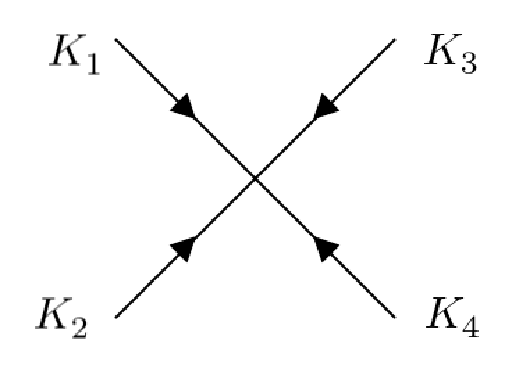
\includegraphics[width=0.20\textwidth, valign=c]{figurer/feynman-diagram/vertex.pdf}
    & = -\lambda \beta
    \delta \left({\sum}_i K_i \right), \\ \nonumber \\
    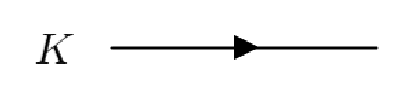
\includegraphics[width=0.2\textwidth, valign=c]{figurer/feynman-diagram/propagator.pdf}
    & = \frac{1}{\beta} D_0(K).
\end{align}
%
Lastly, one has to integrate over internal momenta and divide by the symmetry factor of the diagram $s$, which is described in detail in~
% \cite{Peskin:IntroQFT}.

Calculating $\ex{{S_I}^n}_0$ boils down to the sum of all possible Feynman diagrams with $n$ vertices.
The first example is 
\begin{align}
    \ex{S_I}_0 =
    \frac{1}{8} 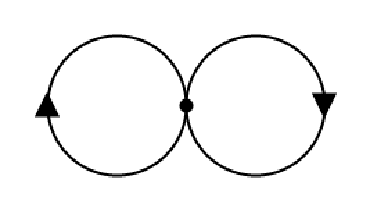
\includegraphics[width=0.20\textwidth, valign=c]{figurer/feynman-diagram/buble.pdf}.
\end{align}

In \autoref{section: path integral}, we saw that the sum of all vacuum diagrams is the exponential of the sum of all \emph{connected} diagrams, so the free energy of the interacting theory is given by
\begin{equation}
    - \beta F = \ln Z_0 + \Sigma(\mathrm{all\,\, connected\,\, diagrams}).
\end{equation}
%

    \section{*Fermions}
\label{section: fermions}


The derivation of the fermionic path integral is similar to the scalar one, but with some slight but important differences.
If $\psi$ and $\bar \psi$ are fermionic spinor fields, relevant relations are~\autocite{laineBasicsThermalField2016}
%
\begin{align}
    \one 
    &=
    \int \D \psi \D \bar \psi \,
    \exp{- \int \dd X \, \bar \psi \psi}
    \ket{\psi} \bra{\psi} \\
    \braket{\bar \psi | \psi } 
    &= \exp{\int \dd X\, \bar \psi \psi}\\
    Z 
    &= \Tr{\hat \rho} 
    = \int \D \psi \D \bar \psi\,
    \exp{- \int \dd X \, \bar \psi \psi} \braket{- \psi | e^{i\beta \hat H} | \psi},
\end{align}
%
The anti-periodic nature of fermion-fields, as mentioned in \autoref{section: imaginary-time formalism}, is due to these differences.
We can verify them by studying the properties of the thermal Greens function.
The thermal Greens function may be written 
\begin{equation}
    D(X_1, X_2) = D(\vec x, \vec y, \tau_1, \tau_2) 
    = \Tr{e^{-\beta H} \psi(\tau_1, \vec x)\psi(\tau_2, \vec y) }.
\end{equation}
In the same way that $i \hat H$ generates the time translation of a quantum field operator through 
$
\hat\varphi(x) = \hat\varphi(t, \vec x) = e^{it\hat H} \hat \varphi(0, \vec x) e^{-it\hat H} 
$, 
the imaginary-time formalism implies the relation
$
    \hat\varphi(X) = \hat\varphi(\tau, \vec x) 
    = e^{\tau\hat H} \hat \varphi(0, \vec x) e^{-\tau \hat H}.
$
Using $\one = e^{\tau \hat H} e^{-\tau \hat H}$ and the cyclic property of the trace, we show that, assuming $\beta>\tau>0$,
\begin{align*}
    D(\vec x, \vec y, \tau, 0)
    % = \bra{\Omega}e^{-\beta \hat H} \T{\varphi(\tau, \vec x) \varphi(0, \vec y)}\ket{\Omega} 
    &= \frac{1}{Z} \Tr{
        e^{-\beta \hat H} \varphi(\tau, \vec x) \varphi(0, \vec y)
    } \\
    % & = \frac{1}{Z} \Tr{
    %     \varphi(0, \vec y) e^{-\beta \hat H} \varphi(\tau, \vec x)
    % } \\
    & = \frac{1}{Z} \Tr{
        e^{-\beta \hat H} e^{\beta \hat H} \varphi(0, \vec y) 
        e^{-\beta \hat H} \varphi(\tau, \vec x)
    } \\
    & = \frac{1}{Z} \Tr{
        e^{-\beta \hat H} \varphi(\vec y, \beta) \varphi(\tau, \vec x)
    } 
    = \nu D (\vec x, \vec y, \tau, 0)
    % = \nu \bra{\Omega}        
    % e^{-\beta \hat H} \T{ \varphi(\tau, \vec x) \varphi( \beta, \vec y) }
    % \ket{\Omega}.
\end{align*}
This implies that $\varphi(0, x) = \nu \varphi(\beta, \varphi)$, where $\nu = \pm 1$ for bosons and fermions respectively, which shows that bosons are periodic in time, as stated earlier, while fermions are anti-periodic.


The Lagrangian density of a free fermion is
\begin{equation}
    \Ell = \bar \psi \left( i \slashed{\partial} - m \right) \psi.
\end{equation}
This Lagrangian is invariant under the transformation $\psi \rightarrow e^{-i \alpha} \psi$, which by Nöther's theorem results in a conserved current
\begin{equation}
    j^\mu = \pdv{\Ell}{(\partial_\mu \psi)} \delta \psi=  \bar \psi \gamma^\mu \psi.
\end{equation}
The canonical momentum corresponding to $\psi$ is
\begin{equation}
    \pi = \pdv{\Ell}{(\partial_0 \psi)} = i \bar \psi \gamma^0,
\end{equation}
and the Hamiltonian density is 
\begin{equation}
    \He = \pi \dot\psi - \Ell
    = \bar \psi (-i\gamma^i\partial_i + m) \psi
\end{equation}
%
In the grand canocical ensamble, we substitute $\He \rightarrow \He - \mu \bar \psi \gamma^0 \psi$, which gives the euclidian Lagrangian
which gives
%
\begin{equation}
    \Ell_E = 
    - \pi \dot\psi + \He(\psi, \pi) - \mu \bar \psi \gamma^0 \psi
    = \bar\psi[\gamma^0 (\partial_\tau - \mu) - i\gamma^i \partial_i + m] \psi,
\end{equation}

With this, the partition function is
%
\begin{align*}
    Z & = \int \D \psi \D \bar \psi
    \exp{
        - \int_\Omega \dd X \, \bar \psi
        \left[
            \gamma_0(\partial_\tau -\mu) -  i \gamma^i \partial_i + m
        \right]
        \psi
    }\\
    % & = C \int \D \tilde \psi\D \tilde {\bar \psi}\,
    % \exp{
    %     - \int_{\tilde \Omega} \dd K \, \tilde {\bar \psi}
    %     \left[
    %         i \gamma_0(\omega_n + i\mu) + i \gamma_i p_i + m
    %     \right]
    %     \tilde \psi
    % } \\
    & = C \int \D \tilde \psi \D \tilde {\bar \psi} \,
    e^{- \langle \tilde {\bar \psi}, D^{-1} \tilde \psi\rangle} 
    = \det(D^{-1}).
\end{align*}
In the second line, we have inserted the Fourier expansion of the field, as defined in \autoref{section: imaginary-time formalism}, and changed variable of integration, as we did for the scalar field.
We then used the Grassmann version of the Gaussian integral,~\autocite{schwartzQuantumFieldTheory2013}
%
\begin{equation}
    \int \dd \bar \theta_i \dd \theta_i \exp{- \theta_i A_{ij}\theta_j} = \det(A).
\end{equation}
%
The linear operator in this case is 
\begin{equation}
    D^{-1} = i \gamma^0 (-i\partial_\tau + i\mu) - (- i \gamma^i) \partial_i + m
    = 
    \beta [i \tilde \gamma_a k_a + m ].
\end{equation}
This equality must be understood as an equality between linear operators, which are represented in different bases.
We introduced the notation $k_a = (\omega_n + i \mu, k_i)$ and use the Euclidean gamma matrices $\tilde \gamma_i$, as defined in \autoref{subsection: Pauli matrices}.
We use the fact that
%
\begin{equation*}
    \det(i\tilde\gamma_a k_a + m)
    = \det(\gamma^5 \gamma^5)
    \det(i\tilde\gamma_a k_a + m)
    = \det[\gamma^5 (i\tilde\gamma_a k_a + m) \gamma^5]
    = \det(-i\tilde\gamma_a k_a + m),
\end{equation*}
%
Let $\tilde D^{-1} = \beta[-i\tilde\gamma_a k_a + m]$, which means we can write
%
\begin{equation}
    Z = \sqrt{\det(D^{-1})\det(\tilde D^{-1})} = \sqrt{\det(D^{-1}\tilde D^{-1})} 
    = \det[\one \beta^2(k_a k_a + m^2)]^{1/2},
\end{equation}
%
where we have used the anti-commutation rule for the Euclidean gamma-matrices, $\{\tilde \gamma_a, \tilde  \gamma_b\} = 2 \delta_{ab}$.
It is important to keep in mind that the determinant here refers to linear operators on the space of spinor functions.
Thus
%
\begin{align}
    \nonumber
    \ln(Z) 
    & = \ln\left\{\det[\one\beta^2(k_a k_a + m^2)]^{1/2}\right\}
    = \frac{1}{2} \Tr{\ln[\one\beta^2(k_a k_a + m^2)]} \\
    & =  2 \int_{\tilde \Omega} \dd K \,  \ln\{ \beta^2[(\omega_n + i\mu)^2 + \omega_k^2]\}.
\end{align}
%
In the last step, we used the fact that the matrix within the logarithm is diagonal.
The matrix part of the trace is trivial and therefore trivial.
Using the fermionic version of the thermal sum from \autoref{section: thermal sum} gives the answer
%
\begin{equation}
    \label{free energy fermions}
    \Eff 
    = -\frac{2}{\beta} \int\frac{\dd^3 k}{(2\pi)^3} \, 
    \left[
        \beta \omega_k
        + \ln\left(1 + e^{-\beta(\omega_k-\mu)}\right)
        + \ln\left(1 + e^{-\beta(\omega_k+\mu)}\right)
    \right].
\end{equation}
%
We see again that the temperature-independent part of the integral diverges, and must be regulated.
There are two temperature-dependent terms, one from the particle and one from the anti-particle.


    
    \chapter{Code}
    \label{appendix: code} 
 
All code is available at: \url{https://github.com/martkjoh/master}.


\section{Integrating the TOV equations}

For numerical integration of the TOV equations, we use SciPy's \texttt{integrate.solve\_ivp}.\footnote{
    Reference available here: \url{https://docs.scipy.org/doc/scipy/reference/generated/scipy.integrate.solve_ivp.html}.
    }
Equations of state are evaluated either as explicit functions if a closed-form is available or as an interpolating function is created using a cubic spline without smoothing.
All code is written using dimensionless variables, and setting $k_1 = k_2 = k_3$.
The TOV equation is then \autoref{TOV dimensionless}
%
\begin{align}
    \odv{\tilde m}{\tilde r} 
    = 3 \tilde r^2 \tilde u, \quad
    \odv{\tilde p}{\tilde r} 
     = - \frac{1}{\tilde r^2} \left(\tilde p + \tilde u\right) 
    \left(3  \tilde r^3 \tilde p + \tilde m\right) 
    \left(1 - \frac{2 \tilde m}{\tilde r}\right)^{-1}.
\end{align}
%
As $r \rightarrow 0$, parts of the TOV equation \autoref{TOV dimensionless} approach a $0/0$-limit, and we must make use of an approximation for numeric evaluation.
The Taylor-expansion of the mass function around $\tilde r = 0$ is
%
\begin{equation}
    \tilde m(r) = \tilde m(0) + \tilde m'(0) \, \tilde r + \frac{1}{2!} \tilde m''(0) \tilde r^2
    + \frac{1}{3!} \tilde m'''(0) \tilde r^3 + \Oh\left(\tilde r^4\right).
\end{equation}
%
One of the boundary conditions is $\tilde m(0) = 0$.
We then use the differential equation for $\tilde m$, \autoref{diff eq mass}, to find
%
\begin{equation}
    \tilde m'(0) = 0, \quad
    \tilde m''(0) = 0, \quad
    \tilde m'''(0) = 6 k_2 \tilde u_0,
\end{equation}
%
where $\tilde u_0 = \tilde u(r = 0)$.
We get an approximation of the TOV equation for $\tilde r \ll 1$ by substituting the $\tilde m$ for its Taylor expansion and including only the leading-order term, which gives
%
\begin{equation}
    \odv{\tilde p}{\tilde r}
    \sim - \tilde r \, \left(\tilde p + \tilde u\right)
    \left( 3 \tilde p + \tilde u_0  \right)
    \left(1 - 2 \tilde u_0 \tilde r^2\right)^{-1}, \quad r\rightarrow 0
\end{equation}
%
For the Newtonian approximation to the TOV equation, we get
%
\begin{equation}
    \odv{\tilde p}{\tilde r} = -\frac{\tilde u \tilde m}{\tilde r^2}
    \sim - \tilde u \tilde u_0 \tilde r,  \quad r\rightarrow 0.
\end{equation}

 

\section{Symbolic calculations in \chpt}
\label{section: symbolic calculations}

Symbolic calculations in \chpt, such as the expansion of the Lagrangian in $\varphi$, were done using the open-source, Python-based case SageMath\footnote{\url{https://www.sagemath.org/}}, and jupyter notebook\footnote{\url{https://jupyter.org/}}.
The calculations consisted of expanding the Lagrangian in a series of $\varphi_a/f$.
The calculations presented in this thesis, in addition to expansions of $\Ell_4$ to second order, can be found in the online repository, at \url{https://github.com/martkjoh/master/tree/main/power_expansion}.



\section{Spherically symmetric metric}

The calculations in \autoref{chapter: GR} were done using a CAS system.
The code is written in Python in a Jupyter notebook.
The full \texttt{.ipynb} file with executable code is available in the repository, at \url{https://github.com/martkjoh/master/blob/main/scripts/TOV/TOV.ipynb}
Below is some of the code, which illustrates the main functions and the outputs.

\includepdf[pages=-,pagecommand={},width=1.3\textwidth]{../scripts/TOV/TOV.pdf}





    \cleardoublepage
    \phantomsection
    \addcontentsline{toc}{chapter}{Bibliography}

    \addtocontents{toc}{
        \vspace*{\fill}
        Sections with (*) are adapted from the specialization project with only minor changes as discussed in the preface.
    }

    % Ensure linebreaks on DOI's in bibliography
    \setcounter{biburlnumpenalty}{1000}
    \setcounter{biburlucpenalty}{1000}
    \setcounter{biburllcpenalty}{1000}


    \printbibliography


\end{document}
